\documentclass{article}

%%%%%%%% CONTROL COMMENTS
\newif\ifcomments
\commentstrue  % change this to false to hide our rainbow comments
%\commentsfalse

%%%%%%%% Packages
\usepackage{amsmath,amsthm}
\usepackage{amssymb,amscd,url,enumerate}
%\usepackage[theorems,skins]{tcolorbox} % for extended euclidean cards
\PassOptionsToPackage{table}{xcolor}\usepackage[theorems,skins]{tcolorbox} % pass options because of package clash
%\usepackage[theorems]{tcolorbox} % for extended euclidean cards
%\usepackage[utf8]{inputenc}
%\usepackage{caption}
%\usepackage{cite}
%\usepackage{xypic}
%\usepackage{tikz}
%\usepackage{tikz-cd}
%\usepackage{amsfonts}
\usepackage{graphicx}
%\usepackage{lipsum}  % removed: unused, and its expl3 dependency makes LaTeXML hang
%\usepackage{xcolor}
%\usepackage{mathrsfs}
\usepackage[margin=1in]{geometry}
%\usepackage{mathtools}
%\usepackage{enumitem}
\usepackage[colorlinks=true]{hyperref}
\usepackage{physics}
\usepackage{nicematrix}
\usepackage{mathtools}

\usepackage{tikz}
\usetikzlibrary{arrows.meta, positioning}

% To make the multiplication tables / Vig square we need this
\usepackage{dcolumn}
\usepackage[table]{xcolor}
\newcolumntype{2}{c}  % simple centred column (was dcolumn's D{.}{}{1.0}; these tables have no decimals)


%%%%%%%% Set Up Theorem-Style Formats %%%%%%%%%%%%%% 
\theoremstyle{plain} 

\newtheorem{theorem}{Theorem} 
\newtheorem{conjecture}[theorem]{Conjecture}
\newtheorem{proposition}[theorem]{Proposition}
\newtheorem{checkin}[theorem]{Concept Check}
\newtheorem{fact}[theorem]{Fact}

\newtheorem{lemma}[theorem]{Lemma}
\newtheorem{corollary}[theorem]{Corollary}
\newtheorem{heuristic}[theorem]{Heuristic}
\newtheorem{philosophy}[theorem]{Philosophy}
\newtheorem{quiz}[theorem]{Quick Quiz}

\theoremstyle{definition}

\newtheorem{definition}[theorem]{Definition}

\theoremstyle{remark}

\newtheorem{remark}[theorem]{Remark}
\newtheorem*{observation}{Observation}
\newtheorem{example}[theorem]{Example}
\newtheorem{problem}[theorem]{Problem}
\newtheorem{question}[theorem]{Question}
\newtheorem*{solution}{Solution}
\newtheorem*{aisolution}{AI Generated Solution (needs review)}

\numberwithin{theorem}{section}



%%%%%%% Comment system control
\let\SS\relax   \DeclareMathOperator{\SS}{SS}
\definecolor{Bittersweet}{rgb}{1.0, 0.44, 0.37}
\definecolor{CornflowerBlue}{rgb}{0.39, 0.58, 0.93}
\definecolor{KateColour}{rgb}{0.3, 0.6, 0.3}%56, 156, 64

\ifcomments
\newcommand{\KS}[1]{\textcolor{violet}{{\sf (Todo:} {\sl{#1})}}}
\else
\newcommand{\KS}[1]{}
\fi

\title{The Alchemy of Mathematical Cryptography}
\author{Katherine E. Stange}


\date{\today}%, Draft \#\VERSION}

\newcommand{\RR}{\mathbb{R}}
\newcommand{\QQ}{\mathbb{Q}}
\newcommand{\FF}{\mathbb{F}}
\newcommand{\ZZ}{\mathbb{Z}}
\newcommand{\NN}{\mathbb{N}}
\newcommand{\CC}{\mathbb{C}}
\newcommand{\PP}{\mathbb{P}}



\begin{document}

\maketitle

\begin{abstract}
This is a work in progress (since 2022) that may become a cryptography textbook aimed at a wide undergraduate audience, including mathematics and computer science majors, with an emphasis on an intuition for the underlying mathematical concepts built through playground experience.  

This is very much a work in progress and frequently in flux.  Corrections are most welcome.  These notes are available for your use, but my preferred method of sharing them is to post a link to this repository:

\begin{centering}
\url{https://www.overleaf.com/project/6303c691a35f843709cd5abd}
\end{centering}
\end{abstract}

\tableofcontents


\section{Introduction \& Overview}

\KS{Some intro to be written.}

\subsection{Classical cryptography}

The use of cryptography is scattered throughout history.  We know of examples from ancient Greeks, Romans, Vikings, and Islam, and cryptography even appears in the Hebrew bible in the form of the Atbash cipher.  Instead of undertaking anything chronological, I will briefly touch on the main mathematical ideas that surfaced before modern times.  The word \textbf{cipher} is typically used to describe an encryption system that works letter-by-letter, bit-by-bit, or perhaps block-by-block, by substitution (replacing the letter, bit or block with something new) or transposition (reordering the letters, bits or blocks).  We will only encounter this type of encryption in the historical section.  For the history of cryptography, see the books:
\begin{enumerate}
	\item \emph{Secret History:  The Story of Cryptology} by Craig P. Bauer
	\item \emph{The Codebreakers:  The Comprehensive History of Secret Communication from Ancient Times to the Internet} by David Kahn.
\end{enumerate}

\subsubsection{Substitution ciphers}

Most abundant in history are examples of \textbf{substitution ciphers}.  These are ciphers in which each letter of the alphabet is replaced with another letter, or a novel symbol.  If this is done in a fixed manner (so that the substitution rule does not change at different positions of the message), this is called a \textbf{monoalphabetic substitution cipher}.  For any encryption method, the original message is called the \textbf{plaintext} and the resulting encrypted message is called the \textbf{ciphertext}.  Thus a substitution cipher is one which replaces each character of the plaintext to obtain the ciphertext.  The first published treatise on substitution ciphers may have been written by Al-Qalqashandi in Egypt in the 1300's (see Kahn's book above).

The simplest and most famous example is the Caesar cipher, attributed to Julis Caesar.  In this system, the alphabet is shifted some number of positions in one direction.  For example, with a shift of one position, `A' becomes `B,' `B' becomes `C' and so on.  For demonstration, this is typically implemented as a double wheel, where one alphabet is rotated relative to the other.  An example is given in Figure~\ref{fig:cipher-wheel}.

\begin{figure}
\begin{center}
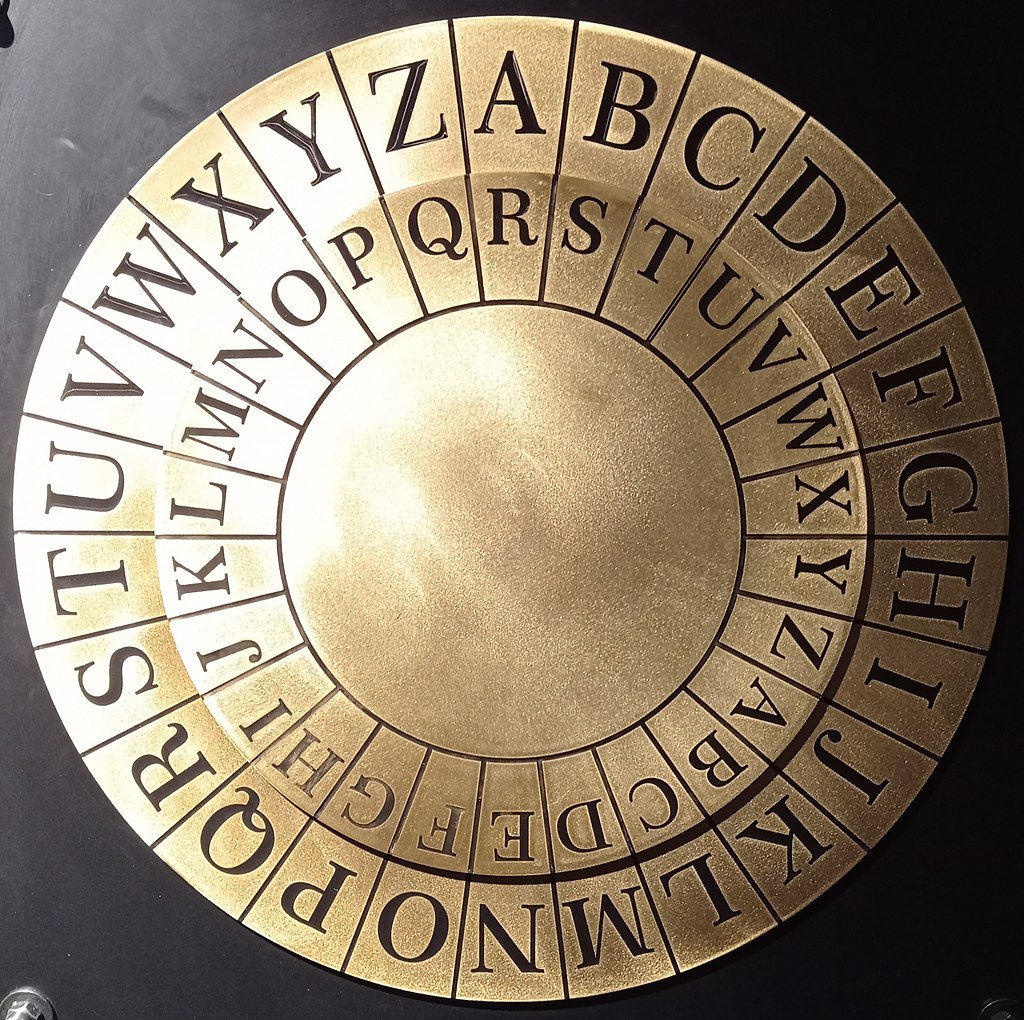
\includegraphics[width=0.3\textwidth]{c-cipher.jpg}
\end{center}
\caption{Image of a Cipherwheel, used for Caesar cipher encryption. 
 With the setting shown here, assuming the outer wheel represents plaintext and inner wheel represents ciphertext, `CIPHER' would encrypt to `TZGYVI'.
     Image:  Subjectiveart, CC BY-SA 4.0 https://creativecommons.org/licenses/by-sa/4.0, via Wikimedia Commons}
\label{fig:cipher-wheel}
\end{figure}



In general, one may use any permutation of the alphabet, not just a cipherwheel rotation.  Or one may use unusual symbols to replace letters, such as the `dancing men' in the eponymous Sherlock Holmes story (\emph{The Adventure of the Dancing Men}, Sir Arthur Conan Doyle).  An interesting example is that of a \textbf{Polybius square} (used for signalling long distances in ancient Greece).  The letters of the alphabet are arranged into a grid (the `Polybius square'), and each letter of the plaintext is then replaced by the coordinates it occupies in the grid (See Figure~\ref{fig:polybius-example}).

\begin{figure}
$$
\begin{array}{c|ccccc}
  & 1 & 2 & 3 & 4 & 5 \\
\hline
1 & A & B & C & D & E \\
2 & F & G & H & I/J & K \\
3 & L & M & N & O & P \\
4 & Q & R & S & T & U \\
5 & V & W & X & Y & Z \\
\end{array}
$$
\caption{Example of a Polybius square.  For example, the letter $B$ is encrypted as $(1,2)$.}
\label{fig:polybius-example}
\end{figure}

In each case, the cipher is encrypted and decrypted with knowledge of a \textbf{secret key}.  The key to the Caesar cipher is the number of positions to shift.  The key to a general monoalphabetic substitution cipher is the list of substitutions for each letter.

\subsubsection{Transposition ciphers}

Another approach to cryptography is not to change the letters of the plaintext at all, but to simply reorder them to obtain the ciphertext.  For example, one might write a message left to right in successive rows to form a square, and then read it off in successive columns to obtain the ciphertext (Figure~\ref{fig:transposition-example}).  A famous example of this type of cipher is known as a \textbf{scytale}.  This is a physical encryption device:  the message is written on a belt and wrapped around a cylinder; then the ciphertext is read up and down the cylinder in rows.  This device was rumoured to have been used by the ancient Greeks.

\begin{figure}
\caption{Example of a transposition cipher}
\label{fig:transposition-example}
\end{figure}

\begin{figure}
\caption{Example of a scytale}
\label{fig:scytale-example}
\end{figure}

Any cipher in which the letters of the message are simply rearranged is called a \textbf{transposition cipher}.  The key to a transposition cipher is also a permutation, but this time on the letters of the plaintext, not the letters of the alphabet.


\subsubsection{Multialphabetic substitution ciphers}

The Vigen\`ere cipher deserves special attention, as it represents a conceptual advance from most other classical cryptograph of the past several millennia.  It was gradually developed in the 1400s and 1500s by a number of people, none of which was Vigen\`ere (as is the case for many named mathematical ideas).  The key insight is that a Caesar cipher would be much more secure if a \emph{different} key were used for each letter of the plaintext.  

It is useful to have on hand a Vigen\`ere square, seen in Figure~\ref{fig:vig-square}.  This shows the alphabet in each of its 26 possible shifted forms.  To begin, we choose a key word.  We could choose, for example, the word `POLLEN.'  Each letter of the key is interpreted as a shift.  The letter `P,' being the 16th letter of the alphabet, represents a shift of 16 positions.  Writing the keyword, repeatedly, above the plaintext, we encrypt each letter of the plaintext with the corresponding shift.  See Figure~\ref{fig:vig-example}

\begin{figure}
\caption{Vigen\`ere square}
\label{fig:vig-square}
\KS{AI: this figure is EMPTY (no content) and its label \texttt{fig:vig-square} is DUPLICATED -- the same label is on the real addition-table figure later (the one that renders as Figure~13). Two figures sharing a label makes the reference ambiguous. Likely fix: delete this empty placeholder and let the reference point to the real Figure~13.}
\end{figure}

\begin{figure}
  \begin{tabular}{c|ccccccccccccccc}
       KEY & 1 & 3 & 2 & 4 & 1 & 3 & 2 & 4 & 1 & 3 & 2 & 4  \\
       \hline
       PLAINTEXT & A & T & T & A & C & K & A & T & D & A & W & N \\
       \hline
       CIPHERTEXT & B & W & V & E & D & N & C & X & E & D & Y & R \\ 
     \end{tabular}
     \caption{Example of the Vigen\`ere cipher \KS{still to be updated}}
\label{fig:vig-example}
\end{figure}

The cryptanalysis of the Vigen\`ere cipher, described as `impossible of translation' as recently as a 1907 \KS{1917?} Scientific American article, is clever, but encryption can be done by hand.  It is even said that Casanova used his masterful cryptanalysis of a lady's secret message to woo her (see \emph{Secret History}).

\subsubsection{The one-time pad}

If one takes the Vigen\`ere cipher to its extreme and uses a keyword whose length matches that of the ciphertext, and which is generated randomly (it is not, for example, an english word), then we obtain something called a \textbf{one-time pad}.  This has the gratifying property of being \emph{truly} secure, in the following sense:  any ciphertext can be made to match with any plaintext by a judicious choice of key.  In other words, if we were to try all keys exhaustively, we would encounter every possible plaintext.  There would be no way to know which was the correct one.

This may be a good moment for some mathematical formalism.  Let us suppose we are working with \textbf{binary bitstrings}, i.e. strings of 1s and 0s.  There's a useful binary operation called \textbf{XOR}, denoted by $\oplus$ and it is defined as follows:  $0 \oplus 0 = 1 \oplus 1 = 0$, $0 \oplus 1 = 1 \oplus 0 = 1$.  With this language, we can define the one-time pad (on binary bitstrings) as follows:  XOR the key with the plaintext, character by character.  See Figure~\ref{fig:onetime-example} for a real-life example from the 1940's.

\begin{figure}
\begin{center}
    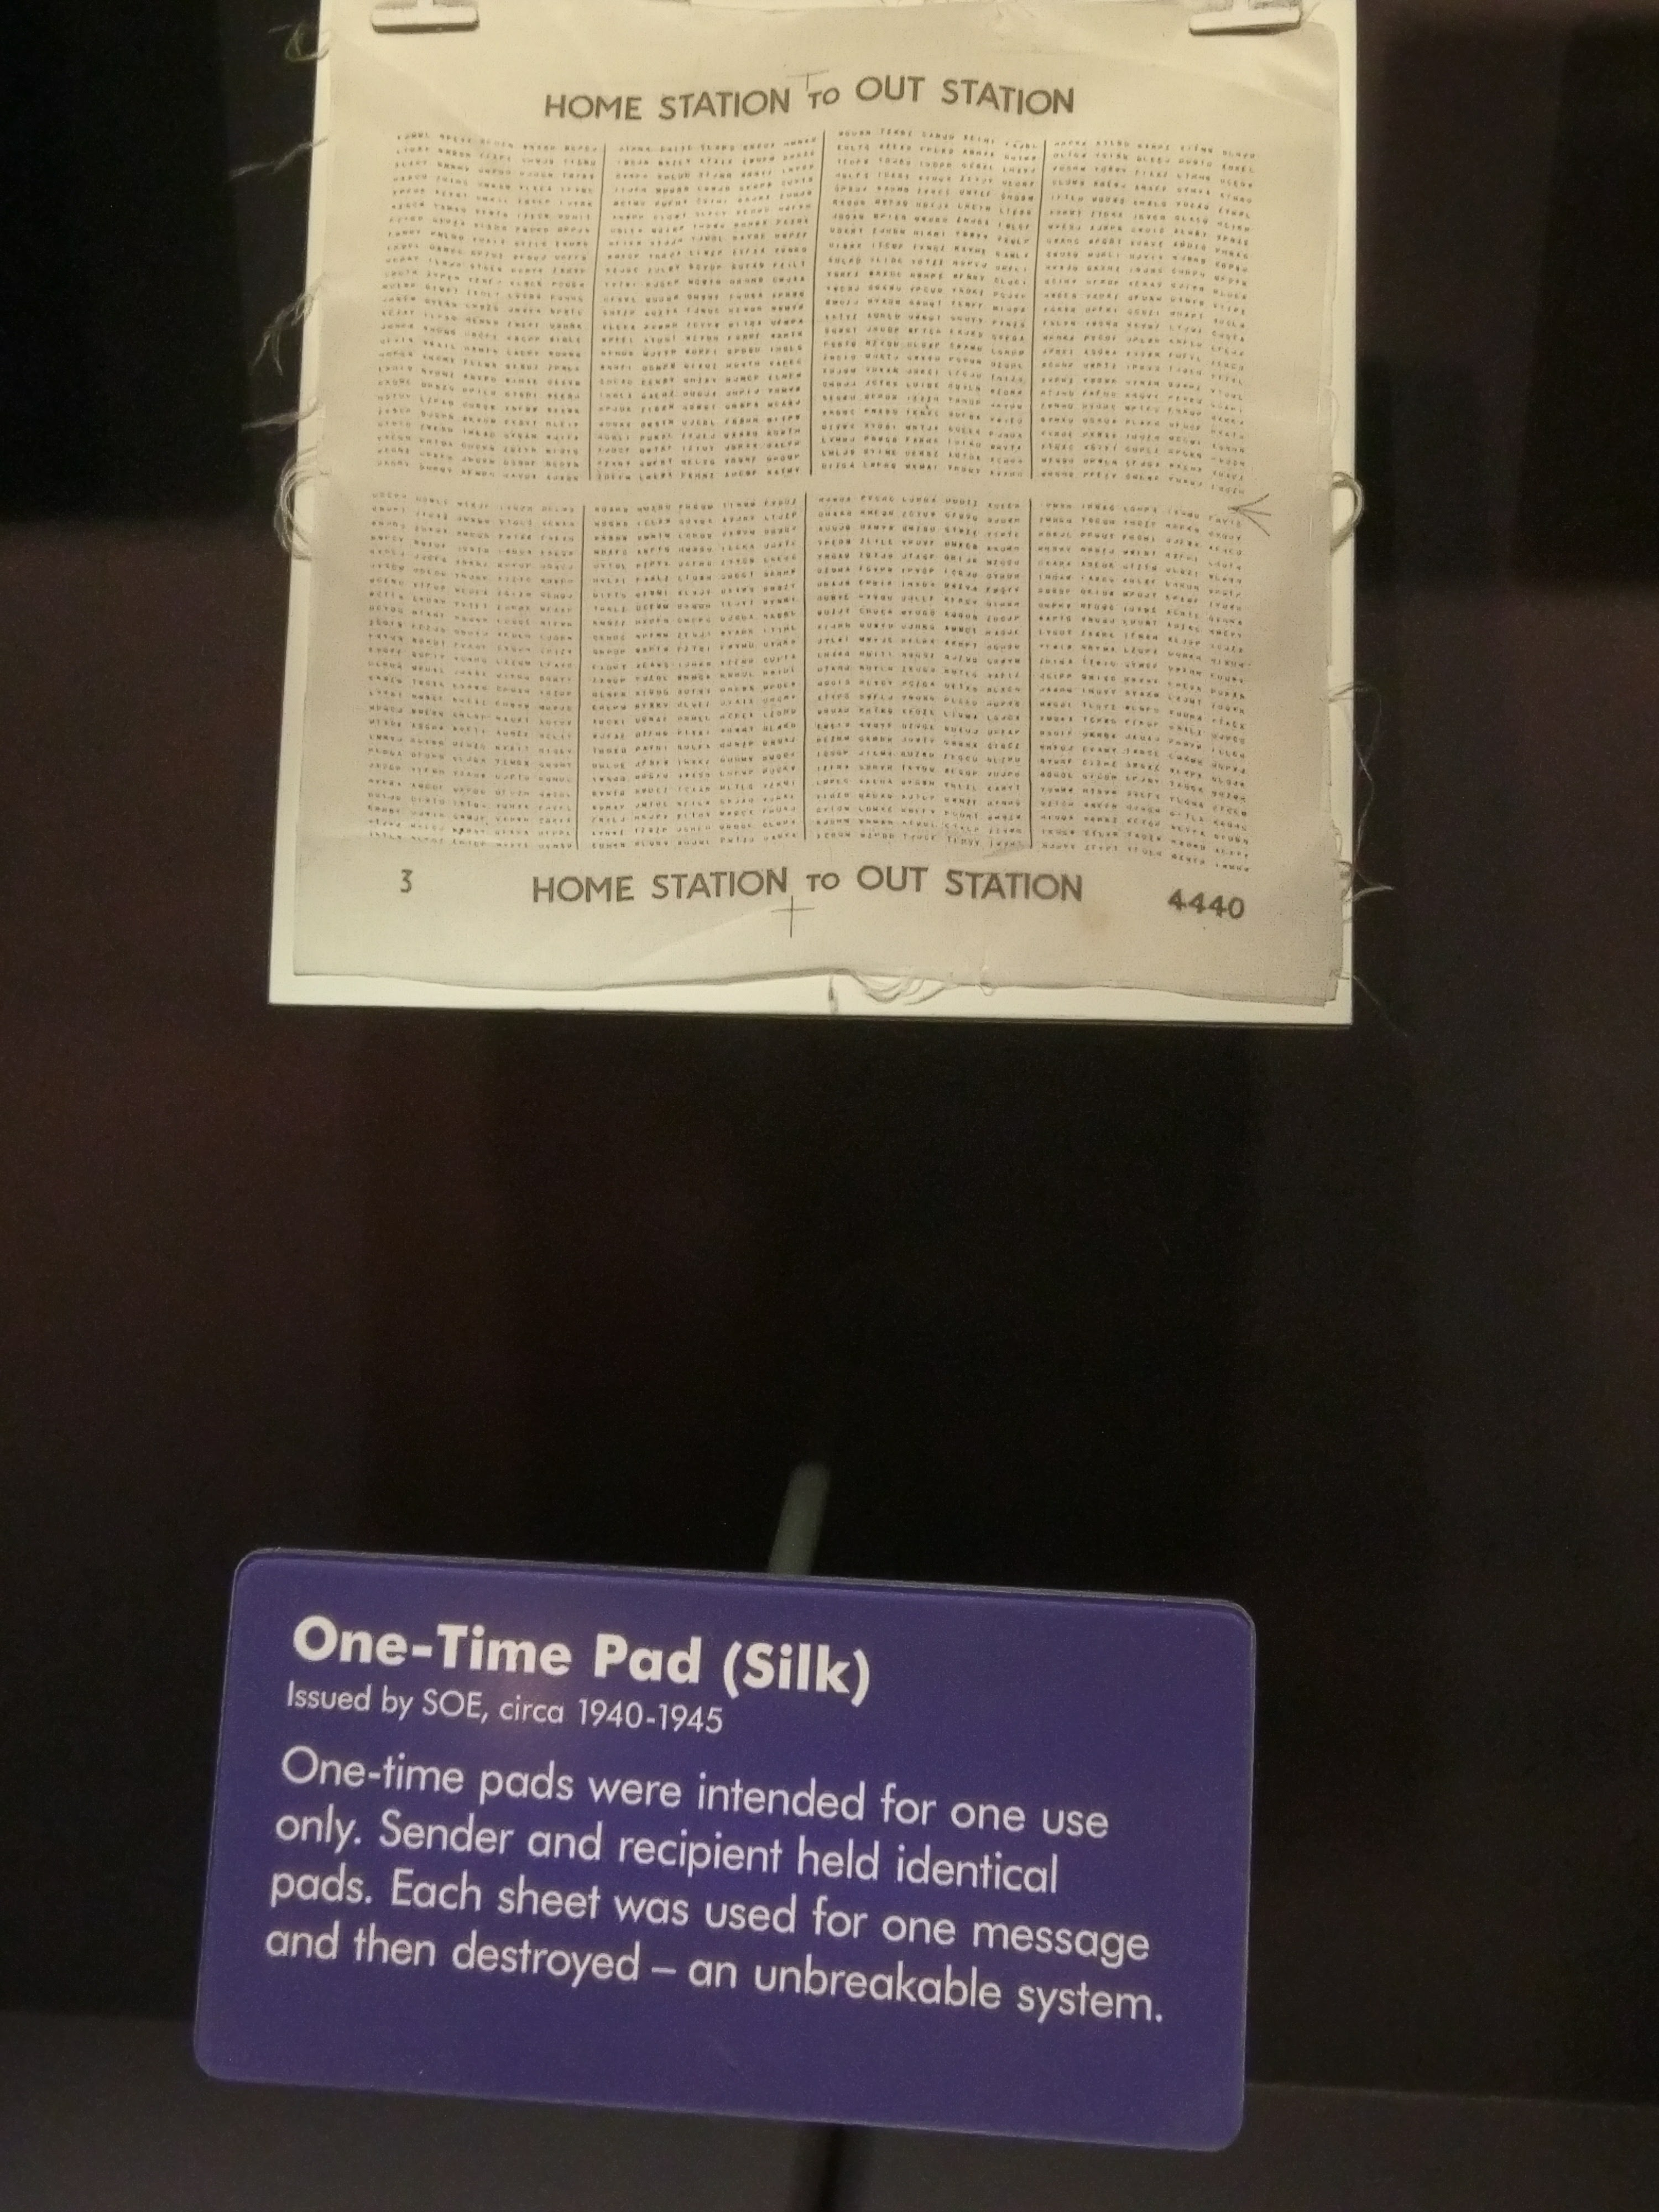
\includegraphics[width=0.6\textwidth]{one-time.jpg}
\end{center}
\caption{Example of a One-Time Pad, used by the Special Operations Executive, which conducted espionage for the British in German-occupied Europe during World War II.  Image by author, Washington Spy Museum.}
\label{fig:onetime-example}
\end{figure}

\begin{theorem}
	Given any ciphertext and plaintext (both binary bitstrings), there is a one-time pad key which encrypts the ciphertext to the plaintext.
\end{theorem}

\begin{proof}
	It is a property of XOR that if $a \oplus b = c$, then $c \oplus b = a$.  Therefore, given a plaintext and ciphertext, we can recover a key which encrypts the plaintext to the ciphertext by taking XOR between plaintext and ciphertext, character-by-character.
\end{proof}
	

\subsubsection{Other old ciphers}

Most ciphers up until world war two were at most combinations of substitution and transposition.  Indeed, in world war one, the ADFGVX cipher was the culmination of cryptography used for the First World War.  It works by first applying a Polybius square in which each letter is replaced with a pair of letters.  Then, the resulting sequence of letters is subject to a simple transposition cipher, which breaks apart the pairs.  This property makes it in part a \textbf{polygraphic substitution cipher}, meaning it replaces characters in groups.  A tutorial on this cipher is available in my video library.  See Figure~\ref{fig:adfgvx-example}.

\begin{figure}

\begin{center}

    \begin{minipage}{.6\textwidth}
        \centering
 \begin{tabular}{c|cccccc}
       & A & D & F & G & V & X \\
       \hline
       A & c & o & 8 & x & f & 4 \\
       D & m & k & 3 & a & z & 9 \\
       F & n & w & 1 & 0 & j & d \\
       G & 5 & s & i & y & h & u \\
       V & p & l & v & b & 6 & r \\
       X & e & q & 7 & t & 2 & g \\
     \end{tabular}

    \end{minipage}%
    \begin{minipage}{.4\textwidth}
        \centering
    
     \begin{tabular}{cccc}
       3 & 4 & 2 & 1 \\
       \hline
       D & G & X & G \\
       X & G & D & G \\
       A & A & D & D \\
       D & G & X & G \\
       F & X & D & G \\
       F & D & F & A
     \end{tabular}


    \end{minipage}
    \vspace{3em}


     Plaintext:  ATTACK AT DAWN \\
     \vspace{1em}

     Step 1:  DG XG XG DG AA DD DG XG FX DG FD FA \\
     \vspace{1em}

     Ciphertext:  GGDGGAXDDXDFDXADFFGGAGXD\\
     \vspace{1em}

   \end{center}
\caption{Example of the ADFGVX cipher}
\label{fig:adfgvx-example}
\end{figure}

Another famous polygraphic cipher is matrix encryption, which is often called a Hill cipher, but sometimes credited to both Levine and Hill during the first half of the twentieth century.  In this system, letters are replaced with their positions in the alphabet (so `A' becomes `1' etc.), and then groups of letters are considered vectors.  Matrices then act on the vectors.  We will see this in Section~\ref{sec:hill}.



\subsubsection{The Enigma Machine}

\KS{To be written}


\subsection{Symmetric-key cryptography}

All the systems discussed so far are \textbf{symmetric key cryptosystems}.  Such a system consists of:

\begin{enumerate}
	\item A \textbf{secret key}, i.e. a piece of information that allows for easy encryption and decryption, secretly shared between sender and receiver.
	\item An \textbf{encryption method}, that uses the \textbf{secret key} to transform the \textbf{plaintext} (the original message, typically in a natural language such as english) into the \textbf{ciphertext} (the encrypted message that looks like gobbledygook to the untrained eye).
	\item A \textbf{decryption method}, that uses the \textbf{secret key} to transform the \textbf{ciphertext} into the \textbf{plaintext}.
\end{enumerate}

There are a few important features of such a cryptosystem.  One is that the secret key must be shared ahead of time in some secretive manner before the system can be used.  In the time before modern cryptography, when these were the only schemes available, big banks would fly a courier with a briefcase handcuffed to his arm:  the briefcase contained the secret key.  \KS{verify this historical claim, which I've read in many places}  The need to obtain shared secret keys before encrypted communication is sometimes called the \textbf{key distribution problem}.

Another important feature, when the scheme is viewed in this abstract manner, is that the security of the system appears closely tied to the \textbf{keyspace}, that is, the set of all possible keys.

For example, in the Caesar cipher, the keyspace consists of the $26$ possible alphabetic shifts, so the keyspace is $\{ 0, 1, 2, \ldots, 25 \}$.  If a keyspace is too small, then an \textbf{exhaustive search} can reveal the key.  In an exhaustive search, the attacker will simply try to decode the ciphertext using each of the keys in the keyspace, one by one.  This will give a number of possible plaintexts, and the attacker must be able to recognise the real plaintext, perhaps because it reads with meaning in a natural language.  Figure~\ref{fig:caesar-exhaustive} shows an exhaustive search attack on a Caesar ciphertext.

\begin{figure}
	\begin{center}
	 \begin{minipage}{0.45\textwidth}
		 \begin{center}
     \begin{tabular}{c|c}
	     key & plaintext \\
       \hline
 0 & WFYDAKZLWPL \\
 1 & XGZEBLAMXQM \\
 2 & YHAFCMBNYRN \\
 3 & ZIBGDNCOZSO \\
 4 & AJCHEODPATP \\
 5 & BKDIFPEQBUQ \\
 6 & CLEJGQFRCVR \\
 7 & DMFKHRGSDWS \\
 8 & ENGLISHTEXT \\
 9 & FOHMJTIUFYU \\
10 & GPINKUJVGZV \\
11 & HQJOLVKWHAW \\
12 & IRKPMWLXIBX \\
      \end{tabular}
      \end{center}
      \end{minipage}
      \begin{minipage}{0.45\textwidth}
	      \begin{center}
     \begin{tabular}{c|c}
	     key & plaintext \\
       \hline
13 & JSLQNXMYJCY \\
14 & KTMROYNZKDZ \\
15 & LUNSPZOALEA \\
16 & MVOTQAPBMFB \\
17 & NWPURBQCNGC \\
18 & OXQVSCRDOHD \\
19 & PYRWTDSEPIE \\
20 & QZSXUETFQJF \\
21 & RATYVFUGRKG \\
22 & SBUZWGVHSLH \\
23 & TCVAXHWITMI \\
24 & UDWBYIXJUNJ \\
25 & VEXCZJYKVOK \\
      \end{tabular}
\end{center}
      \end{minipage}
\end{center}
\caption{An exhaustive search through the keyspace of a Caesar cipher}
\label{fig:caesar-exhaustive}
\end{figure}

Therefore, the security of a symmetric key cryptosystem is bounded in terms of its keyspace:  a small keyspace necessarily means a weak system.  But a big keyspace does not guarantee a strong system.  Even with a very large keyspace, a clever \textbf{cryptanalyst} (one who attempts to break a cryptosystem) may have a more efficient algorithm than an exhaustive search.  An example of this is the alphabetic cipher mentioned in Section \KS{GIVE SEC}.  For english, the keyspace consists of all possible permutations of 26 roman letters.  That's a space of size $26!$ ($26$ factorial).  That means there are more than $400,000,000,000,000,000,000,000,000$ possible keys.  Trying one per nanosecond (a nanosecond may by time for a couple of instructions on a modern laptop) that will take over $12,000,000$ millennia.

Despite this large keyspace, however, solving alphabetic ciphers is a popular pastime, as evidenced by the Cryptogram found in many weekend newspapers, which is essentially an alphabetic ciphertext without a key provided; the goal is to obtain the plaintext.  This amusement dates to the middle ages (Wikipedia).  Methods vary, but are typically based on patterns inherent in the target language.  For example, in english, the letter `E' is the most frequently used letter, so one may guess that the most frequently occurring letter in the ciphertext should correspond to `E.'  Proceeding by guessing and familiarity with english allows many people to solve these in a pleasantly passed half hour over breakfast.

Therefore the security of a symmetric key cryptosystem is affected by the size of the keyspace and the availability of efficient \textbf{cryptographic attacks}, or methods that may reveal the plaintext, without use of the secret key.  Exhaustive search is a cryptographic attack that is always available, but one hopes for something faster.



\subsection{The notion of complexity}

\textbf{Complexity} refers to the efficiency of an algorithm, as a function of its inputs.  
With the discussion of the previous section in mind, we see that to discuss security is really to discuss complexity:  is there an \textbf{efficient} cryptographic attack algorithm?  The notion of efficiency is the notion of speed:  how long does it take?  In principle, any system can be broken by exhaustive search of the keyspace, but if this is expected to take longer than the time before the sun dies, then it is not a practical algorithm.  Instead, we want something that will break the system on a human timescale, such as hours or, at worst, years.

To capture this idea, we formalize complexity in terms of the notion of runtime.  This could be measured in seconds or CPU cycles or a related unit.  As technology advances, runtimes decrease.  So we find it mathematically expedient to discuss \textbf{asymptotic complexity}.  That is, \emph{how does the runtime grow as a function of the input size?}  

An example is perhaps the best way to explain this concept.  The \textbf{input size} is the number of bits it takes to put in the question the computer must solve.  If the problem is factoring, then the input is the integer $N$ which is to be factored.  To write down $N$ and feed it to the computer, however, you need to write it in binary or decimal notation (you don't write $N$ ticks in a row on a piece of paper!).  In this case the \emph{number of digits} is the size -- that's how much space it takes to write down the number to input to the computer.  The number of binary digits of $N$ is approximately $\log_{2}(N)$.

Let's say we wish to find a factor of the integer $N$ by trial division.  The \textbf{trial division} algorithm proceeds as follows:  for each integer $k$ less than or equal to $\sqrt{N}$, compute $N/k$ and see if the remainder is zero (in other words, if it divides evenly).  If it divides evenly, we have found a factor.  If $N$ has a \textbf{proper factor} (something other than itself and $1$), then this algorithm will find it, since one of its proper factors will be\footnote{Can you see why?  Pause and convince yourself that this must be true.  What if both were bigger than $\sqrt{N}$?} less than $\sqrt{N}$.

The \textbf{asymptotic runtime} or \textbf{asymptotic complexity} is the time taken as a function of that input size, as the input size grows.  For our example algorithm, the time taken is $\sqrt{N}$ trial divisions.  Assume for simplicity for the moment that a trial division takes a constant amount of time\footnote{this is not true, but we will ignore that for now}.  Then the time taken as a function of input size is $\sqrt{N}$ steps as a function of $\log_2(N)$.  If we let $X := \log_2(N)$ represent the input size, then\footnote{the notation $:=$ means that I am defining the symbol on the left to be the quantity on the right} we have $N = 2^X$ and we obtain a runtime of $\sqrt{N} = N^{1/2} = 2^{X/2} = \sqrt{2}^X$.  This is an \emph{exponential} function in $X$, so we say that trial division is an \textbf{exponential algorithm}.

Exponential algorithms are horrendous things.  In our example, if it takes time $T$ to factor something of $b$ bits, then it takes time $T^2$ to factor something of $2b$ bits.  Double the bits means the square of the amount of time!  Triple the bits and you must cube the time taken.  This means that we can write down, on a single piece of paper, integers that are so large we expect humankind will never be able to factor them\footnote{Well, with our current tools, anyway!  Quantum computers are on the horizon.}.

\subsection{The advent of public-key cryptography}

The earliest public-key cryptographic schemes could, in principle, have been known to the ancients.  They rely only on modular arithmetic.  However, it may be hard, from our modern perspective, to appreciate just how \emph{incredibly} counterintuitive the question is.  It is simply the case that no one every asked it.  The question is:

\emph{How can Bob send Alice an encrypted message without first having set up a secret key?}

After all, if there is no secret key, then everything that Alice obtains from Bob is visible to any eavesdropper.  So of course this is not possible!

Except that it is.

The loophole is that Alice can share some information for Bob to use in aiming his message at Alice.  This is called Alice's \textbf{public key}.  She generates it in a special way that also generates a \textbf{private key} which she keeps secret, and which allows her to decrypt the message.  Bob encrypts his message using Alice's public key, resulting in a ciphertext that can only be decrypted with Alice's private key.

Even now, you may be skeptical.  \KS{Insert some history of PKE}

Therefore, I will convince you by demonstrating the first of our public-key schemes.  

\subsubsection{Key exchange}

Our first public-key scheme isn't strictly a type of encryption, but rather a type of \textbf{key exchange}, a protocol which results in Alice and Bob sharing some secret information (which they can then use as a secret key for a symmetric encryption such as Caesar cipher, modern symmetric encryption, or whatever their hearts' desire).  A key exchange can more formally be defined as a \textbf{protocol} (or procedure) performed by Alice and Bob, in communication, which allows both Alice and Bob to compute a piece of shared secret information, in such a way that an eavesdropped Eve, privy to all communication between Alice and Bob, cannot feasibly compute the same secret information.  They cannot control this information ahead of time, e.g. they cannot conspire to make it an english word, and it will typically be a random string.

Here's a sort of failed first attempt at a key exchange:

\begin{enumerate}
	\item Alice chooses a private key $a$ (an integer)
	\item Bob chooses a private key $b$ (an integer)
% AI-FLAGGED ORIGINAL:
%	\item Alice makes a public key $2a$ and sends it to Bob.
%	\item Bob makes a public key $2b$ and sends it to Alice.
	\item Alice makes a public key $5a$ and sends it to Bob.
	\item Bob makes a public key $5b$ and sends it to Alice.
\KS{Fixed by AI: the rest of this example (steps below and the Eve/division-by-$5$ discussion) uses public keys $5a$ and $5b$; the multiplier here should be $5$, not $2$, for internal consistency.}
	\item Alice can compute (Alice's private key)x(Bob's public key) $= a(5b) = 5ab$.
	\item Bob can compute (Bob's private key)x(Alice's public key) $= b(5a) = 5ab$.
\end{enumerate}

At the end of this process, Alice and Bob both have the information $5ab$.  The information that passed between them was only their public keys, $5a$ and $5b$.  However, you, dear reader, have necessarily seen the flaw in this setup:  if Eve, our eavesdropper, has the information of $5a$ and $5b$, she can compute $5ab$ by computing (Bob's public key)x(Alice's public key)/5 $= (5b)(5a)/5 = 5ab$.

So this hasn't gotten us anywhere.  But observe that Eve's process is \emph{different} than Alice's or Bob's:  she needed to know how to do division by $5$.  What if that were computationally intensive, so much so that she couldn't do it during her lifetime?

This is what motivates the \textbf{Diffie-Hellman Key Exchange}. This is a slight variation on the work above, but where Eve's job is computationally intensive.  It involves taking exponents modulo a large prime $p$.  If you are not familiar with modular arithmetic, you can either visit Section REF SEC, or, for the moment, you can take for granted that there's a special world of arithmetic called `mod p' which has some properties I'll explain below (but you will certainly want to learn modular arithmetic for the rest of this course!).

\begin{enumerate}
	\item Alice chooses a private key $a$ (an integer).
	\item Bob chooses a private key $b$ (an integer).
	\item Alice makes a public key $\alpha^a \pmod p$ and sends it to Bob.
	\item Bob makes a public key $\alpha^b \pmod p$ and sends it to Alice.
	\item Alice can compute $\text{(Bob's public key)}^\text{(Alice's private key)} \pmod p = (\alpha^{a})^b \pmod p = \alpha^{ab} \pmod p$.
	\item Bob can compute $\text{(Alice's public key)}^\text{(Bob's private key)} \pmod p = (\alpha^{b})^a \pmod p = \alpha^{ab} \pmod p$.
\end{enumerate}

Now Eve must turn the information of $\alpha^a$ and $\alpha^b$ into the information of $\alpha^{ab}$ to break the system.  It turns out this problem, called the \textbf{Computational Diffie-Hellman Problem}, appears to have high complexity.  That is, no one knows a fast algorithm for it.  So Eve can't break this system (as far as we know).
However, computing $\alpha^a$ and the other exponents in the algorithm \emph{does} have fast algorithms (low complexity), so all these computations can be done very quickly.  Otherwise this wouldn't be a practical scheme, i.e. one we can use in reality on the hardware we have.  In fact, this scheme is very practical and is in use around the world ADD STATISTICS. 

It is exactly this disparity between the complexity of performing the key exchange and the complexity of breaking the key exchange that provides the security of this key exchange scheme.  Unfortunately, we don't actually \emph{know} that the Computational Diffie-Hellman Problem is difficult!  We are fairly confident only because many researchers (mathematicians and computer scientists) have tried to come up with an efficient algorithm, but have failed.  In other words, the security of the modern internet is based only on a \emph{conjecture}.

This is not an unusual state of affairs.  In fact, all of the modern cryptography in use today is based on such assurances.  We trust it only because many people have tried to break it and failed.



\subsection{Hard cryptographic problems}

What makes modern public-key cryptography possible is the notion of a \textbf{hard cryptographic problem}.  By `problem,' we mean a type of computation, such as long division, or factoring.  For cryptography, a problem should be, in its generic state, something for which we do not know efficient algorithms.  Some of the most important hard problems we will discuss in the course are informally stated as follows:

\begin{enumerate}
	\item \textbf{Factoring:}  Given an integer $n$, determine its factorization.
	\item \textbf{Discrete Logarithm:}  Given $\alpha$ and $\alpha^x$ modulo $p$, determine $x$.
	\item \textbf{Shortest Vector Problem:}  Given a basis for a high-dimensional lattice, determine a short vector.
\end{enumerate}

Each of these forms the basis of important cryptographic protocols in use today, and if you can solve any of these with an efficient algorithm (we will discuss exactly what `efficient' means in these contexts later), then you would up-end the entire modern world overnight.  It is possible that someone, somewhere, may do exactly this, any day.

\subsubsection{The basic protocols:  key exchange, encryption, and digital signatures}

Once you have a hard problem, you can build a \textbf{cryptographic protocol}, or a procedure to accomplish a cryptographic task.  The three most important cryptographic tasks are as follows.  In each protocol, keys appear in the form of a pair (secret key, public key).  We call this a \textbf{key pair}.

\begin{enumerate}
	\item \textbf{Key Exchange:}  Two parties, Alice and Bob, in communication, use their key pairs to compute a shared piece of secret information not obtainable without at least one of their secret keys.  This is used by your web-browser during the \textbf{handshake} procedure initiated when setting up a session with a secure (https://) server.  The secret information is then used for symmetric key cryptography which encrypts all the traffic between server and client.
	\item \textbf{Encryption:}  One party, Alice, produces a key pair, and then a second party, Bob, uses Alice's public key to encrypt data which can only be decrypted using Alice's secret key.  In some older protocols (TLS 1.2 now deprecated but still in use), RSA encryption is used to agree upon a shared key for symmetric cryptography to encrypt the session.
	\item \textbf{Digital signature:}  One party, Alice, produces a key pair, and uses the secret key to generate a signature attached to a given document.  Any other party, Bob, can verify the signature using Alice's public key.  No third party can forge the signature without access to Alice's private key.  Each web server obtains and displays a certificate of its identity, ownership of the domain name, public key, etc. (this constitutes the document), digitally signed by a trusted authority called a \textbf{certification authority} (almost half the market share belongs to IdenTrust).  Digital signatures are also a workhorse in the bitcoin blockchain.
\end{enumerate}

The landscape of cryptography protocols includes many many more functionalities.  As an example, recent work concerns \textbf{homomorphic encryption}, which is encryption that preserves the structure of data without access to the data itself, e.g. in an encrypted spreadsheet, you may be able to add columns without decrypting.  This allows for a non-trusted party to store and manipulate your data without ever actually accessing it.  For example, you could store genomes on a server and ask the server to perform computationally intensive machine learning on the encrypted data -- all without the server ever having access to the genomes.  Most real-world protocols (like the TLS handshake your browser performs when connecting to an https:// website) use a (sometimes quite complicated) combination of key exchange, encryption, and digital signatures.  At this level, cryptography becomes engineering:  the use of a suite of tools to build a machine with certain functionality.  In this course, we will focus mainly on the `big three' tools above, and their mathematical underpinnings.

\subsection{Cryptanalysis:  breaking things}

\begin{quote}
\emph{“Codemaking is more important, codebreaking is more fun.” – Ed Giorgio. (The Cryptographers’ Panel | USA 2015 RSA Conference)}
\end{quote}

What the cryptographer creates, the cryptanalyst destroys.  The cryptanalyst's role is to invent new and creative ways to break the lovely mathematical protocols forged by cryptographers.  But the cryptanalyst's role is crucial:  without cryptanalysis, we cannot have confidence in cryptographic systems.  Just as you wouldn't trust a phone case that hasn't survived a toddler in testing, new cryptosystems are only trusted after they have survived years of scrutiny by the most dedicated and clever cryptanalysts.


\begin{figure}
\begin{center}
    \includegraphics[width=0.6\textwidth]{bletchleytools.jpg}
\end{center}
\caption{Homemade cryptanalysis tools from Bletchley Park.  Image by Katherine E. Stange, London Science Museum, on loan from GCHQ.}
\label{fig:bletchley-tools}
\end{figure}


There is no wrong way to break a cryptosystem:  a break is a break.
 Some attacks exploit the basic mathematical structure of the protocol.  Some exploit the implementation or hardware itself; these are often called \textbf{side-channel attacks}.  Many, such as the famous Heartbleed attack, exploit implementation bugs.  And usually the most effective route to break a cryptosystem, as XKCD points out (https://xkcd.com/538/), may be human engineering. 

\begin{center}
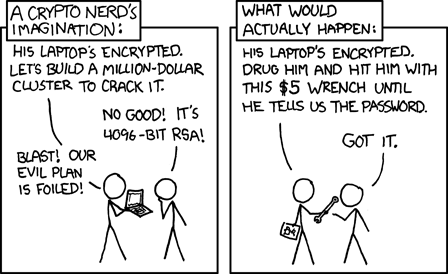
\includegraphics[width=0.6\textwidth]{security.png}\\
(Image from XKCD, https://xkcd.com/538/, Creative Commons Attribution Non-Commercial License, https://creativecommons.org/licenses/by-nc/2.5/)
\end{center}
 
Kerckhoffs stated a famous principal of modern cryptography:

\begin{quote}
 \emph{“A cryptographic system should be secure even if everything about the system, except the key, is public knowledge.” — Auguste Kerckhoffs}
 \end{quote}

You probably know a neighbour who keeps their front door key under a flowerpot.  Suppose they have five flowerpots by their front door.  The only thing keeping them safe is that most people don't know that they are using PottyCrypto\texttrademark.  As soon as someone knows they use this system, they only need to check five pots.  Better security is provided by a combination lock.  That's visible as soon as you walk up to the door -- everyone knows what system your security is based on.  But there may be thousands of combinations to try.

 In other words, the security of a system should not depend on keeping its \emph{design} a secret.  Only the \emph{key} is to be kept secret.  Systems which follow this rule, and survive cryptanalysis, will be considered more secure.
 Sometimes this principle is shortened to the pithy phrase:  ``Avoid security through obscurity.''
 
 In practice, this means that you should assume an adversary knows not only what algorithm you are using, but can read the code you are using to run it, has knowledge of the chip it runs on, etc.  Any of these things could be exploited by a cryptanalyst.


  In this text we will focus on mathematical cryptanalysis, that is, the creation of algorithms which can attack the underlying hard cryptographic problem, or the mathematics of the protocol itself.  In this context, we will assume the programmer has done a perfect job and introduced no bugs, that the hardware is not leaking information about the CPU cycles, etc.  (If only such a utopia existed.)
  
An adversary (one who hopes to break a system) may have access to many different types of information.  For example:

\begin{enumerate}
	\item A single ciphertext.
	\item Example pairs of ciphertexts and plaintexts.
	\item Examples of multiple signatures generated from a single key pair.
	\item The ciphertext of a chosen plaintext (for example, if the adversary has access to the encryption machine and can encrypt a message with it).
	\item ... and many more possible situations.
\end{enumerate}

When we discuss the \textbf{security} of a cryptosystem we mean its resistance against an attacker deciphering an arbitrary ciphertext.  In this model, called a \textbf{ciphertext-only attack}, the cryptosystem is known -- but not the key! --, an arbitrary ciphertext is provided, and the attacker must discover the plaintext.  To break the cryptosystem is to invent an algorithm which will succeed with reasonable success probability on random such ciphertexts.

There are terms for the security of a cryptosystem against an adversary with other particular pieces of information or particular capabilities.  For example, a \textbf{chosen-plaintext attack} is one in which the attacker has access to the encryption machine, in the sense that they can encrypt plaintexts of their choice, to gather information about the key, before attempting to decipher the ciphertext.

\begin{figure}
	\begin{center}
\small
\setlength{\tabcolsep}{2pt}
\begin{tabular}{|c|c|c|c|c|c|c|c|c|c|c|c|c|c|c|c|c|c|c|c|c|c|c|c|c|c|c|c|}
  A & B & C & D & E & F & G & H & I & J & K & L & M & N & O & P & Q & R & S & T & U & V & W & X & Y & Z \\
  0 & 1 & 2 & 3 & 4 & 5 & 6 & 7 & 8 & 9 & 10 & 11 & 12 & 13 & 14 & 15 & 16 & 17 & 18 & 19 & 20 & 21 & 22 & 23 & 24 & 25 \\
\hline\hline
  $8.2$ & $1.5$ & $2.8$ & $4.3 $ & $12.7 $ & $2.2 $ & $2.0 $ & $6.1 $ & $7.0 $ & $0.2 $ & $0.8$ & $4.0$ & $2.4 $ &  $6.7 $ &  $7.5 $&  $1.9 $ &  $0.1 $ &  $6.0 $ &  $6.3 $ &  $9.1 $ &  $ 2.8  $ & $ 1.0 $ & $ 2.3  $ &  $0.1  $ &  $2.0 $ &  $0.1  $ \\
\hline
\end{tabular}
\end{center}
\caption{Standard english letter frequencies in percentage.}
\label{fig:frequencies}
\end{figure}






\begin{quote}
    \emph{“Codebreaking is an art, and codemaking is a science.” – Adi Shamir. (The Cryptographers’ Panel | USA 2015 RSA Conference)}
\end{quote}

\subsection{Randomness}

\KS{To be written.  Meanwhile enjoy some quotes.}

\begin{quote}
    \emph{“Anyone who attempts to generate random numbers by deterministic means is, of course, living in a state of sin.” — John von Neumann}
\end{quote}

\begin{quote}
    \emph{“Random numbers should not be generated with a method chosen at random.” — Donald Knuth}
\end{quote}


\subsection{Living with quantum computers}

\KS{To be written}

\section{Modular arithmetic, the discrete logarithm, and Diffie-Hellman key exchange}

\subsection{Modular arithmetic}

You are likely already familiar with modular arithmetic from your experience with an analog wall clock.  If I agree to meet you two hours after 11 o'clock, you know that this will be 1 o'clock.  The analog wall clock ignores multiples of 12.  Working in this way is called working \textbf{modulo} 12.  There is nothing special about the number twelve; we may work modulo any integer.

\begin{definition}
Let $a$ and $b$ be integers.  We say that
\[
a \equiv b \pmod n
\]
whenever $a = b + nk$ for some integer $k$ (out loud, we say ``$a$ is equivalent to $b$ modulo $n$'' or ``$a$ is congruent to $b$ modulo $n$'').  More informally, that is to say, whenever $a$ and $b$ differ by a multiple of $n$, or whenever $a$ and $b$ have the same remainder upon division by $n$.
\end{definition}

For example\footnote{Whenever you meet a mathematical definition, you should create some examples and non-examples for yourself.}, $12 \equiv 2 \pmod 5$ and $-1 \equiv 3 \pmod 4$, but $0 \not\equiv 1 \pmod 2$.  We will henceforth assume that $n > 1$, since $n \le 1$, although well-defined, does not provide any extra utility.

It is sometimes helpful to imagine modular arithmetic as a wall clock (Figure~\ref{fig:7-clock}).  The usual infinite integer number line can be thought of as being wrapped around this clock in a spiral, so that every integer lands on one of the $n$ possible numbers painted on the clock.  These painted numbers are typically taken to be $\{ 0, 1, 2, 3, \ldots, n-1 \}$ (notice that we include zero and not $n$ itself), and this set\footnote{In a more mathematical formulation, the residues represent equivalence classes of integers.  For example, $0 \pmod n$ should be thought of as the infinite set of integers $\{ k \in \ZZ : n \mid k \}$.  In this course, where we are more concerned with practical matters, we will not focus on this.} is called the set of \textbf{residues modulo $n$}.  If $k$ is equivalent to one of these residues, say $a$, then we say that \textbf{$k$ has residue $a$ modulo $n$}.  

\begin{checkin}
    Use Figure~\ref{fig:7-clock} to show that $7 \equiv -3 \pmod{5}$.
\end{checkin}
\begin{aisolution}
Both numbers land on the same ray of the clock: $7 = 5\cdot 1 + 2$ sits on the ray labelled $2$, and $-3 = 5\cdot(-1) + 2$ also sits on the ray labelled $2$.  Equivalently, $7 - (-3) = 10 = 2\cdot 5$ is a multiple of $5$, so $7 \equiv -3 \pmod 5$.
\end{aisolution}


We use the notation $\ZZ/n\ZZ$ for the set of residues modulo $n$, or the set of `notches' of the clock.  This is a finite set.  If $n$ is equal to a prime $p$, we also write $\FF_p$ (this is in anticipation of our work with finite fields in Section\KS{whatever later chapter}).  Let's record this as a formal definition.


\begin{definition}
	The residues modulo $n$ are denoted $\ZZ/n\ZZ$.  Explicitly,
	\[
		\ZZ/n\ZZ := \{ 0, 1, 2, \ldots, n-1 \}.
	\]
\end{definition}

Every integer is equivalent modulo $n$ to exactly one element of $\ZZ/n\ZZ$.  

\begin{remark}
   If we were being more formal, we would define $\ZZ/n\ZZ$ to be a set of \emph{equivalence classes}, e.g. the residue $1$ should really be thought of as the set of all things congruent to $1$ modulo $n$, i.e. $\{ 1 + kn: k \in \ZZ \}$.  But for us, it's enough to think of them as the residues or remainders.
\end{remark}

\begin{checkin}
    Write out $\ZZ/10\ZZ$ and $\ZZ/3\ZZ$.\footnote{Answers: $\ZZ/10\ZZ = \{0,1,2,3,4,5,6,7,8,9\}$; $\ZZ/3\ZZ = \{ 0,1,2\}$.}
\end{checkin}
\begin{aisolution}
We list the residues $0,1,\ldots,n-1$:
\[
\ZZ/10\ZZ = \{0,1,2,3,4,5,6,7,8,9\}, \qquad \ZZ/3\ZZ = \{0,1,2\}.
\]
\end{aisolution}

It is typical to \textbf{reduce} integers modulo $n$ to one of the $n$ elements of $\ZZ/n\ZZ$.   So, for example, $15 \equiv 0 \pmod{5}$ since it is a multiple of $5$; and $1999999992 \equiv 2 \pmod{10}$ since reducing modulo $10$ is the same as taking the final digit.  

\begin{checkin}
    Reduce $77772$ modulo $7$ (by pure thought).  Hint:  take out obvious multiples of $7$.\footnote{Answer: $2$ (since $77770$ is an obvious multiple of $7$).}
\end{checkin}
\begin{aisolution}
Note $77770 = 7 \cdot 11110$ is a multiple of $7$, so $77772 = 77770 + 2 \equiv 2 \pmod 7$.
\end{aisolution}

\begin{checkin}
    Reduce  $1200004$ modulo $3$ (by pure thought).\footnote{Answer: Since $12$ is a recognizable multiple of $3$, $1200004 \equiv 4 \equiv 1 \pmod{3}$.}
\end{checkin}
\begin{aisolution}
Since $1200000 = 3\cdot 400000$ is a multiple of $3$, we have $1200004 \equiv 4 \equiv 1 \pmod 3$.  (As a check, the digit sum is $1+2+4 = 7 \equiv 1 \pmod 3$.)
\end{aisolution}

Reducing into this `standard' set makes it easier to compare integers and see if they are equivalent modulo $n$.  Since $70 \equiv 0 \pmod{5}$ and $143 \equiv 3 \pmod{5}$, we know that they are not equivalent modulo $5$.



\begin{figure}
\begin{center}
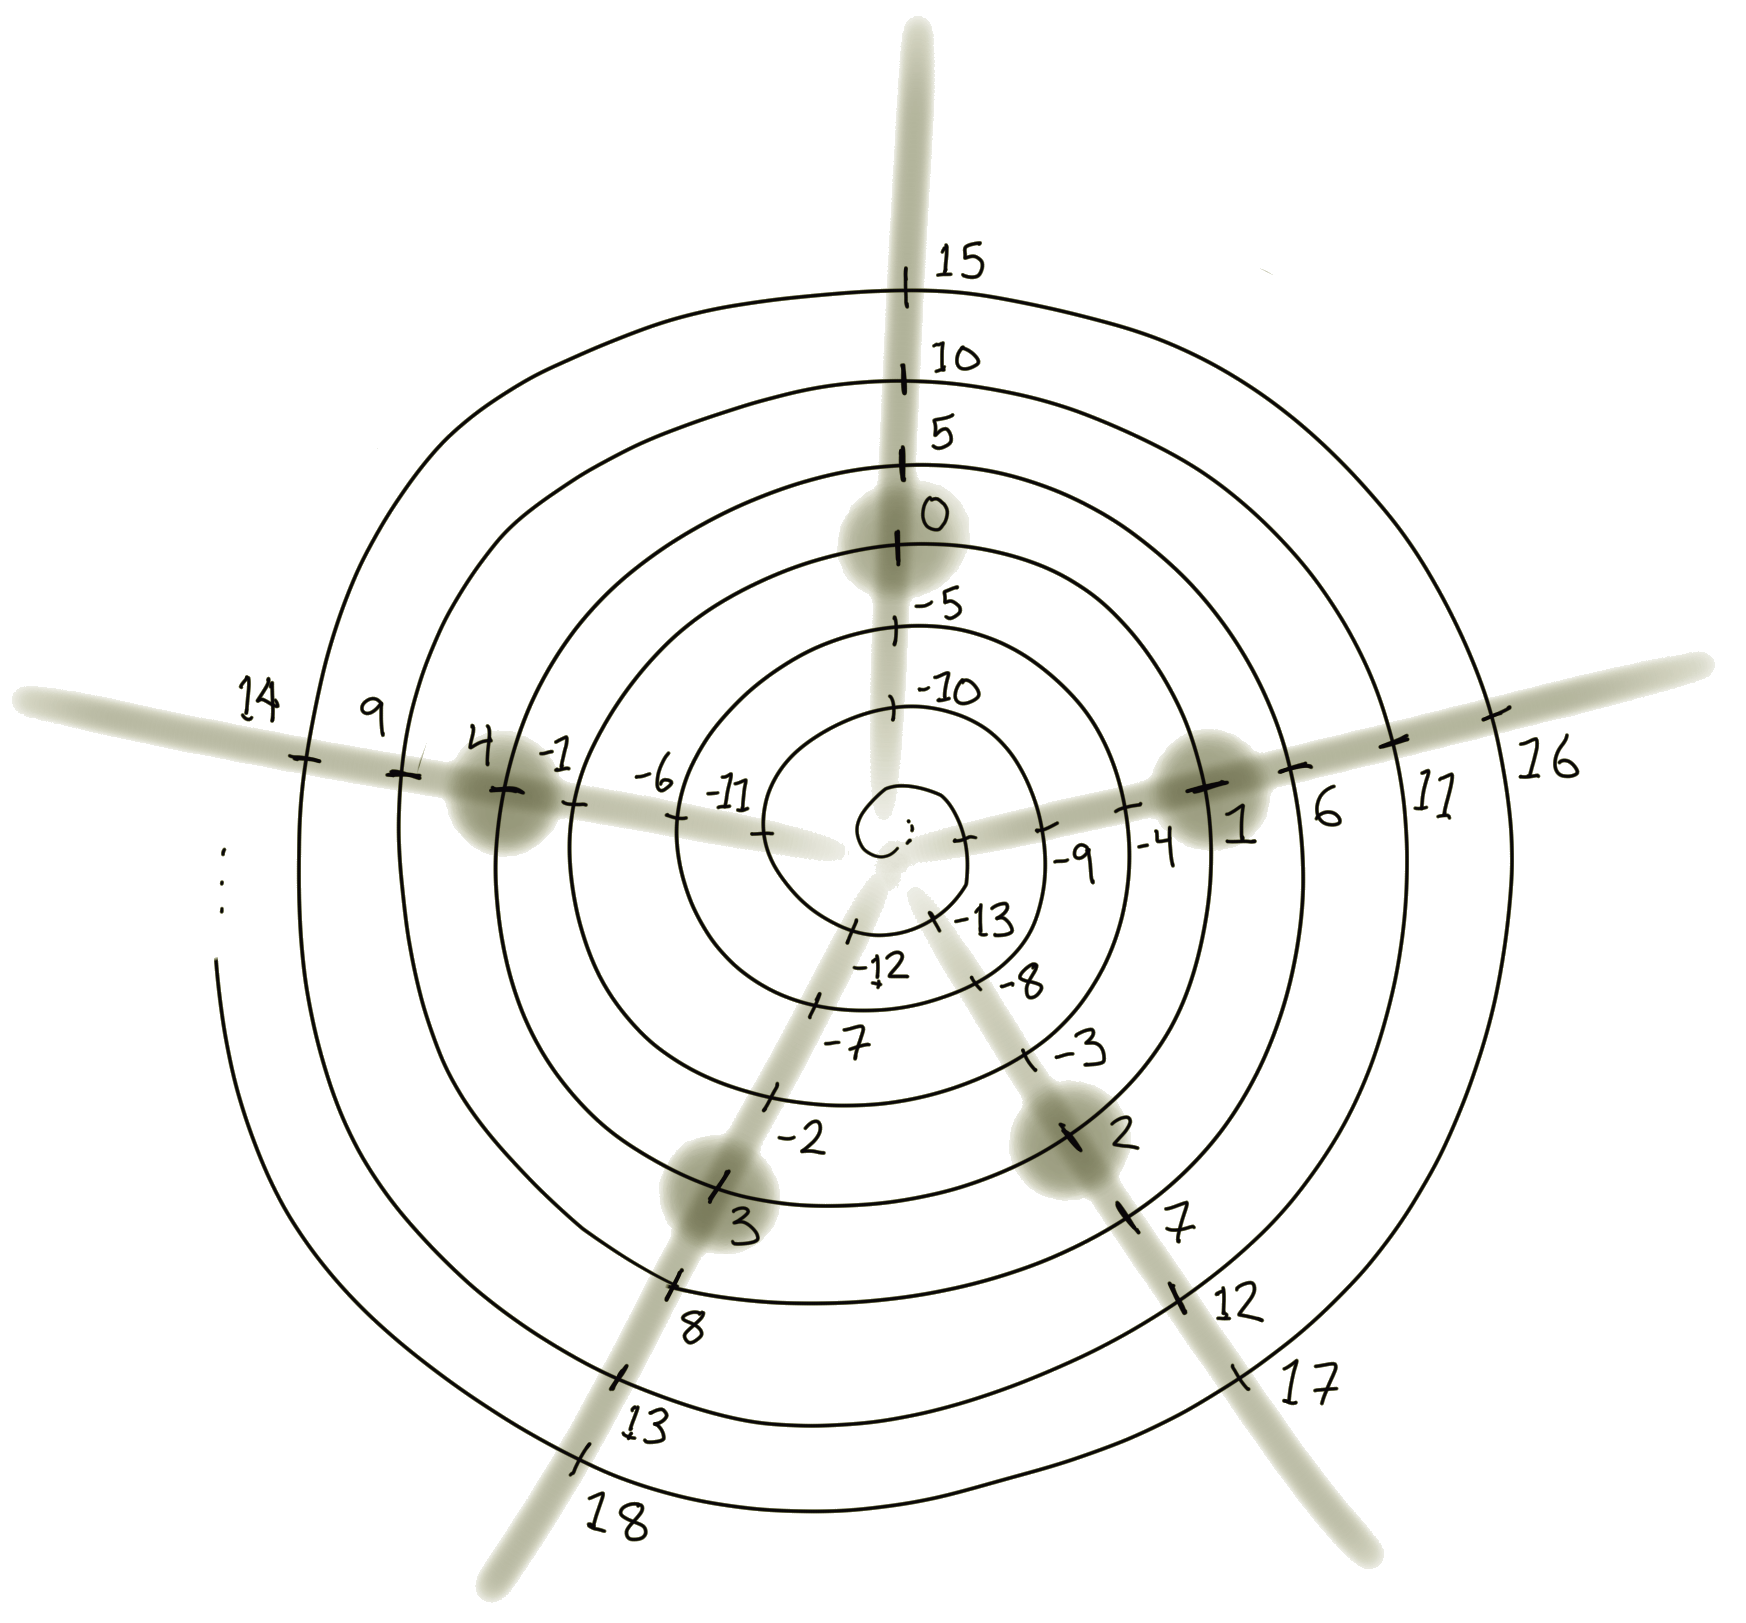
\includegraphics[width=0.4\textwidth]{wind-up.png}
\hspace{2em}
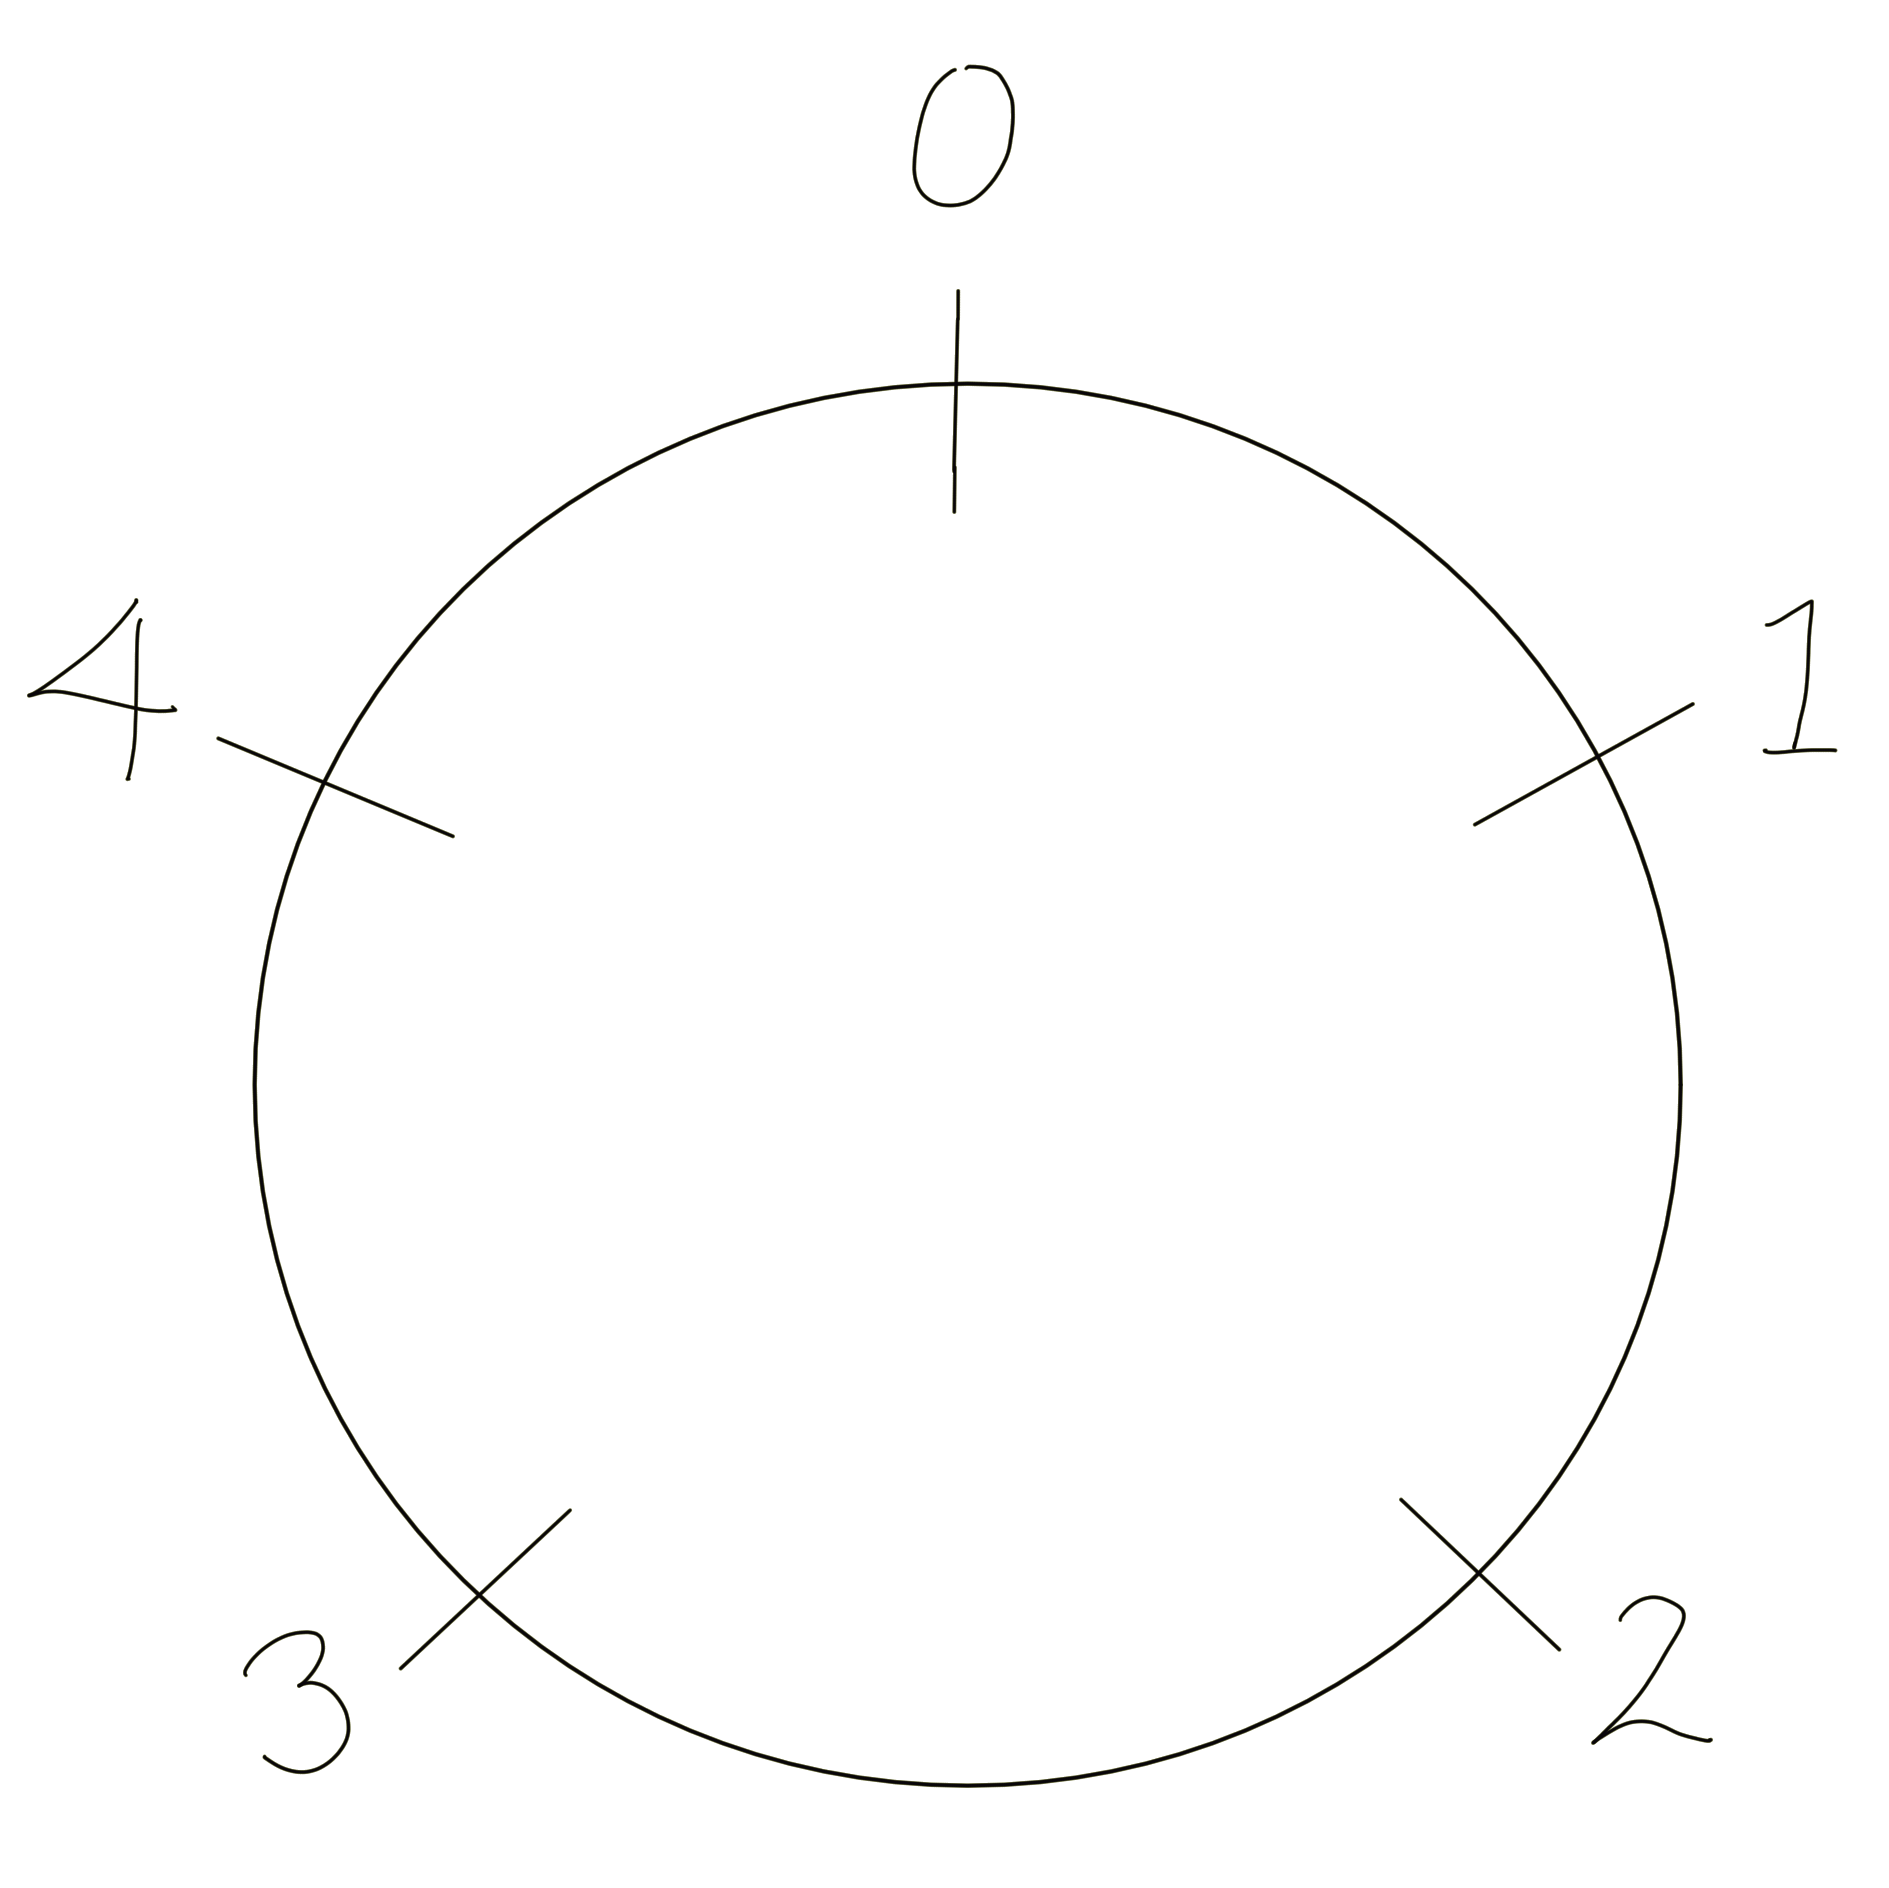
\includegraphics[width=0.3\textwidth]{clock.png}
\end{center}
\caption{An illustration of arithmetic modulo $5$ as a `clock.'  The integer number line can be thought of as wrapped around the clock, so that every integer hits one of the finitely many clock positions.  In this clock, the numbers $\ldots$, $-1$, $4$, $9$, $14$, $\ldots$ are all on the same `ray', so they are all equivalent modulo $5$.  We write $-1 \equiv 4 \equiv 9 \pmod{5}$ etc.  We choose the numbers $0,1,2,3,4$ to represent each ray.}
\label{fig:7-clock}
\end{figure}

The main theorem of modular arithmetic states that addition and multiplication on the regular integers `descend' to the integers modulo $n$.

\begin{theorem}
	\label{thm:well-def-mod}
	Suppose that $a_1, a_2, b_1, b_2, n \in \ZZ$.
	Suppose that $a_1 \equiv b_1 \pmod n$ and $a_2 \equiv b_2 \pmod n$.  Then $a_1 + a_2 \equiv b_1 + b_2 \pmod n$ and $a_1a_2 \equiv b_1b_2 \pmod n$.
\end{theorem}

Stated informally, this asserts that we can define addition and multiplication on $\ZZ/n\ZZ$ without problems:  if we reduce the summands before summation, or the result afterward, we will obtain the same result.  Similarly, if we reduce the factors before multiplication, or the result afterward, we will obtain the same result.
As an example of the theorem in action\footnote{Whenever you meet a Theorem, you should test it out with actual values or mathematical examples, to see it happen.}, we may take $n=5$, $a_1 = 16$, $b_1 = 1$, $a_2 = -3$, $b_2 = 2$.  Then, the hypotheses are verified:  $16 \equiv 1 \pmod 5$ and $-3 \equiv 2 \pmod 5$.  Thus, we expect the conclusion to be verified.  Indeed, $a_1 + a_2 = 13$ and $b_1 + b_2 = 3$, and these are indeed equivalent\footnote{I leave it to the reader to check the second assertion of the conclusion, that concerning multiplication.} modulo $5$.

\begin{checkin}
    Verify that the example just given, the second conclusion of the Theorem (about multiplication) also holds.\footnote{Answer:  $a_1a_2 = -48 \equiv -8 \equiv 2 \pmod{5}$ and $b_1b_2 = 2 \equiv 2 \pmod{5}$.}
\end{checkin}
\begin{aisolution}
With $a_1 = 16$, $a_2 = -3$, $b_1 = 1$, $b_2 = 2$: the product $a_1a_2 = -48 = -50 + 2 \equiv 2 \pmod 5$, while $b_1 b_2 = 1\cdot 2 = 2 \equiv 2 \pmod 5$.  The two products agree modulo $5$, confirming $a_1a_2 \equiv b_1b_2 \pmod 5$.
\end{aisolution}

\begin{proof}[Proof of Theorem~\ref{thm:well-def-mod}]
	Under the hypotheses given\footnote{That $a_1, a_2, b_1, b_2, n \in \ZZ$ and $a_1 \equiv b_1 \pmod n$ and $a_2 \equiv b_2 \pmod n$.}, $b_1 = a_1 + k_1n$ and $b_2 = a_2 + k_2n$, for some integers $k_1, k_2 \in \ZZ$.  Then $b_1 + b_2 = a_1 + a_2 + (k_1+k_2)n \equiv a_1+a_2 \pmod{n}$ and $b_1b_2 = (a_1+k_1n)(a_2+k_2n) = a_1a_2 + n(k_1a_2+k_2a_1 + nk_1k_2) \equiv a_1a_2 \pmod{n}$.  Therefore the conclusions are satisfied.
\end{proof}

The upshot is that modular arithmetic can be very efficient, which is important for cryptographic implementation.  Computations which may look daunting can be done very quickly, because reduction modulo $n$ can be applied during intermediate steps.  For example, working modulo $10$, we can immediately observe that
\[
	1000000000000001^{3000000} \equiv 1^{3000000} \equiv 1 \pmod{10}.
\]
If you gave this computation to a poorly programmed compute, it would attempt to multiply out the gigantic exponent before reducing modulo $10$, resulting in an overflow error.

This is a common trick on high-school math contests.  Here's another example, this time modulo $3$:
\[
	1200002 + 3333333332^{10} \equiv 2 + 2^{1000} \equiv 2 + (2^2)^{500} \equiv 2 + 1^{500} \equiv 2 + 1 \equiv 0 \pmod{3}.
\]
In general these require a bit of creativity.  In both examples above, observe\footnote{Whenever you see the word `observe' in a math textbook, it's an invitation to verify something for yourself; in this example, explain how the rest of this sentence applies to each of the foregoing examples.} that the computation was aided by rearranging to find a base, like $1$ or $-1$, whose powers we understand easily because they have a pattern.

\begin{checkin}
    Compute $1313131312^{50000} \pmod{13}$ (by pure thought).\footnote{Answer: $1313131312 \equiv 12 \equiv -1$, so $1313131312^{50000} \equiv (-1)^{50000} \equiv 1 \pmod{13}$.}
\end{checkin}
\begin{aisolution}
First reduce the base: $1313131313 = 13\cdot 101010101$ is a multiple of $13$, so $1313131312 \equiv -1 \equiv 12 \pmod{13}$.  Then
\[
1313131312^{50000} \equiv (-1)^{50000} \equiv 1 \pmod{13},
\]
since the exponent $50000$ is even.
\end{aisolution}

\begin{checkin}
    Compute $3^{50000} \pmod{8}$ (by pure thought).\footnote{Answer: $3^2 \equiv 9 \equiv 1 \pmod{8}$, so $3^{50000} \equiv (3^2)^{25000} \equiv 1^{25000} \equiv 1 \pmod{8}$.}
\end{checkin}
\begin{aisolution}
Since $3^2 = 9 \equiv 1 \pmod 8$ and $50000 = 2\cdot 25000$ is even,
\[
3^{50000} = (3^2)^{25000} \equiv 1^{25000} \equiv 1 \pmod 8.
\]
\end{aisolution}

Later we will see other ticks for dealing with large exponents.  Informally, the complexity of modular addition and multiplication is a simple\footnote{actually a polynomial; we will discuss this later} function of the modulus itself, since things are quickly reduced into that range.

\subsubsection{Warning!  Don't reduce the exponents modulo $n$.}

Observe these two computations:
\[
3^7 \equiv 3^4 \cdot 3^3 \equiv 9^2 \cdot 3^3 \equiv 81 \cdot 27 \equiv 1 \cdot 7 \equiv 2 \pmod{5}.
\]
but
\[
3^2 \equiv 9 \equiv 4 \pmod{5}.
\]
From this we observe an important counterpoint to Theorem~\ref{thm:well-def-mod}:

\begin{philosophy}
    When working modulo $n$, it is \textbf{not} in general ok to reduce an exponent.
\end{philosophy}

In the example above, $7 \equiv 2 \pmod{5}$ but $3^7 \not\equiv 3^2 \pmod{5}$.  Reducing the exponent is not safe!



\subsection{Classic cryptosystems based on modular arithmetic}

\subsubsection{Caesar cipher}

The Caesar cipher is best viewed as a cryptosystem based on modular arithmetic modulo $26$.  If we identify each letter of the roman alphabet with a residue modulo $26$, then we can express encryption with respect to a secret shift $s$ as the function\footnote{The notation $\mapsto$ is an alternate notation for a map.  The notation $f(x) = x^2$ can be written as $f: x \mapsto x^2$; they both denote the same function.}
\[
	\text{encryption}: m \mapsto m + s \pmod{26},
\]
and then the corresponding decryption is
\[
% AI-FLAGGED ORIGINAL:
%\text{decryption}: c \mapsto c - x \pmod{26}.
\text{decryption}: c \mapsto c - s \pmod{26}.
\]
\KS{Fixed by AI: the secret shift is $s$ (encryption is $m \mapsto m+s$), so decryption must subtract $s$, not the undefined $x$.}
Then the \textbf{plaintext space}, \textbf{ciphertext space} and keyspace are all equal to $\ZZ/26\ZZ$ (although we think of this as the roman alphabet).  Figure~\ref{fig:vig-square} shows the addition table of $\ZZ/26\ZZ$ written in this way.

\begin{figure}
	\begin{center}
\setlength{\tabcolsep}{5pt}
\renewcommand\arraystretch{1.3}
\setlength\doublerulesep{0pt}
\small
\rowcolors{2}{gray!25}{white}
\begin{tabular}{rr||*{26}{2|}}
& & A & B & C & D & E & F & G & H & I & J & K & L & M & N & O & P & Q & R & S & T & U & V & W & X & Y & Z \\
& $\times$ & 0 & 1 & 2 & 3 & 4 & 5 & 6 & 7 & 8 & 9 & 10 & 11 & 12 & 13 & 14 & 15 & 16 & 17 & 18 & 19 & 20 & 21 & 22 & 23 & 24 & 25 \\
\hline\hline
A & 0 & A & B & C & D & E & F & G & H & I & J & K & L & M & N & O & P & Q & R & S & T & U & V & W & X & Y & Z \\
\hline
B & 1 & B & C & D & E & F & G & H & I & J & K & L & M & N & O & P & Q & R & S & T & U & V & W & X & Y & Z & A \\
\hline
C & 2 & C & D & E & F & G & H & I & J & K & L & M & N & O & P & Q & R & S & T & U & V & W & X & Y & Z & A & B \\
\hline
D & 3 & D & E & F & G & H & I & J & K & L & M & N & O & P & Q & R & S & T & U & V & W & X & Y & Z & A & B & C \\
\hline
E & 4 & E & F & G & H & I & J & K & L & M & N & O & P & Q & R & S & T & U & V & W & X & Y & Z & A & B & C & D \\
\hline
F & 5 & F & G & H & I & J & K & L & M & N & O & P & Q & R & S & T & U & V & W & X & Y & Z & A & B & C & D & E \\
\hline
G & 6 & G & H & I & J & K & L & M & N & O & P & Q & R & S & T & U & V & W & X & Y & Z & A & B & C & D & E & F \\
\hline
H & 7 & H & I & J & K & L & M & N & O & P & Q & R & S & T & U & V & W & X & Y & Z & A & B & C & D & E & F & G \\
\hline
I & 8 & I & J & K & L & M & N & O & P & Q & R & S & T & U & V & W & X & Y & Z & A & B & C & D & E & F & G & H \\
\hline
J & 9 & J & K & L & M & N & O & P & Q & R & S & T & U & V & W & X & Y & Z & A & B & C & D & E & F & G & H & I \\
\hline
K & 10 & K & L & M & N & O & P & Q & R & S & T & U & V & W & X & Y & Z & A & B & C & D & E & F & G & H & I & J \\
\hline
L & 11 & L & M & N & O & P & Q & R & S & T & U & V & W & X & Y & Z & A & B & C & D & E & F & G & H & I & J & K \\
\hline
M & 12 & M & N & O & P & Q & R & S & T & U & V & W & X & Y & Z & A & B & C & D & E & F & G & H & I & J & K & L \\
\hline
N & 13 & N & O & P & Q & R & S & T & U & V & W & X & Y & Z & A & B & C & D & E & F & G & H & I & J & K & L & M \\
\hline
O & 14 & O & P & Q & R & S & T & U & V & W & X & Y & Z & A & B & C & D & E & F & G & H & I & J & K & L & M & N \\
\hline
P & 15 & P & Q & R & S & T & U & V & W & X & Y & Z & A & B & C & D & E & F & G & H & I & J & K & L & M & N & O \\
\hline
Q & 16 & Q & R & S & T & U & V & W & X & Y & Z & A & B & C & D & E & F & G & H & I & J & K & L & M & N & O & P \\
\hline
R & 17 & R & S & T & U & V & W & X & Y & Z & A & B & C & D & E & F & G & H & I & J & K & L & M & N & O & P & Q \\
\hline
S & 18 & S & T & U & V & W & X & Y & Z & A & B & C & D & E & F & G & H & I & J & K & L & M & N & O & P & Q & R \\
\hline
T & 19 & T & U & V & W & X & Y & Z & A & B & C & D & E & F & G & H & I & J & K & L & M & N & O & P & Q & R & S \\
\hline
U & 20 & U & V & W & X & Y & Z & A & B & C & D & E & F & G & H & I & J & K & L & M & N & O & P & Q & R & S & T \\
\hline
V & 21 & V & W & X & Y & Z & A & B & C & D & E & F & G & H & I & J & K & L & M & N & O & P & Q & R & S & T & U \\
\hline
W & 22 & W & X & Y & Z & A & B & C & D & E & F & G & H & I & J & K & L & M & N & O & P & Q & R & S & T & U & V \\
\hline
X & 23 & X & Y & Z & A & B & C & D & E & F & G & H & I & J & K & L & M & N & O & P & Q & R & S & T & U & V & W \\
\hline
Y & 24 & Y & Z & A & B & C & D & E & F & G & H & I & J & K & L & M & N & O & P & Q & R & S & T & U & V & W & X \\
\hline
Z & 25 & Z & A & B & C & D & E & F & G & H & I & J & K & L & M & N & O & P & Q & R & S & T & U & V & W & X & Y \\
\hline
\end{tabular}
\end{center}
\caption{Vigen\`ere Square (addition table modulo $26$).}
\label{fig:vig-square}
\end{figure}

\subsubsection{Affine cipher}
Viewing the encryption function as a formula in modular arithmetic, we come naturally to what is called the \textbf{affine cipher}.  For this cipher, we choose a modulus $n$, and then the key $(\alpha,\beta)$ consists two residues $\alpha, \beta \in \ZZ/n\ZZ$.  With this secret, the encryption function is
\[
	\text{encryption}: m \mapsto \alpha m + \beta \pmod{26},
\]
In order to understand the decryption function, we need to understand how to `undo' multiplication by $\alpha$.  Take a look at Figure~\ref{fig:mult-table-modn}, which shows the multiplication table modulo $26$.  The column under the letter corresponding to a residue $k$ is actually a table showing the effect of multiplication-by-$k$.  Examining this table, we observe that multiplication-by-$k$ is bijective for all the odd $k$ except for $13$.  So at least we expect that the encryption can be reversed.  In other words, from this we can conclude that no two plaintexts will go to the same ciphertext.  In fact, this is a general principle worth recording:
\[
	\text{An encryption function should be injective.}
\]

As an example, consider the affine cipher given by $\alpha=2$, $\beta=0$ in $\ZZ/5\ZZ$.  The encryption function is $x \mapsto 2x$, shown in this table:

\begin{tabular}{c|c}
	m & 2m \\
	\hline
	1 & 2 \\
	2 & 4 \\
	3 & 1 \\
	4 & 3 \\
\end{tabular}

This is clearly a bijective function, so it has an inverse, which can be used for decryption.  Interestingly, the inverse function is given by $x \mapsto 3x$, shown in this table:

\begin{tabular}{c|c}
	c & 3c \\
	\hline
	1 & 3 \\
	2 & 1 \\
	3 & 4 \\
	4 & 2 \\
\end{tabular}

It's remarkable that multiplication by $2$ is `undone' by multiplication by $3$.


\begin{figure}
	\begin{center}
\small
\rowcolors{2}{gray!25}{white}
\begin{tabular}{rr||*{26}{2|}}
& & A & B & C & D & E & F & G & H & I & J & K & L & M & N & O & P & Q & R & S & T & U & V & W & X & Y & Z \\
& $\times$ & 0 & 1 & 2 & 3 & 4 & 5 & 6 & 7 & 8 & 9 & 10 & 11 & 12 & 13 & 14 & 15 & 16 & 17 & 18 & 19 & 20 & 21 & 22 & 23 & 24 & 25 \\
\hline\hline
A & 0 & 0 & 0 & 0 & 0 & 0 & 0 & 0 & 0 & 0 & 0 & 0 & 0 & 0 & 0 & 0 & 0 & 0 & 0 & 0 & 0 & 0 & 0 & 0 & 0 & 0 & 0 \\
\hline
B & 1  & 0 & 1 & 2 & 3 & 4 & 5 & 6 & 7 & 8 & 9 & 10 & 11 & 12 & 13 & 14 & 15 & 16 & 17 & 18 & 19 & 20 & 21 & 22 & 23 & 24 & 25 \\
\hline
C & 2 & 0 & 2 & 4 & 6 & 8 & 10 & 12 & 14 & 16 & 18 & 20 & 22 & 24 & 0 & 2 & 4 & 6 & 8 & 10 & 12 & 14 & 16 & 18 & 20 & 22 & 24 \\
\hline
D & 3 & 0 & 3 & 6 & 9 & 12 & 15 & 18 & 21 & 24 & 1 & 4 & 7 & 10 & 13 & 16 & 19 & 22 & 25 & 2 & 5 & 8 & 11 & 14 & 17 & 20 & 23 \\
\hline
E & 4 & 0 & 4 & 8 & 12 & 16 & 20 & 24 & 2 & 6 & 10 & 14 & 18 & 22 & 0 & 4 & 8 & 12 & 16 & 20 & 24 & 2 & 6 & 10 & 14 & 18 & 22 \\
\hline
F & 5 & 0 & 5 & 10 & 15 & 20 & 25 & 4 & 9 & 14 & 19 & 24 & 3 & 8 & 13 & 18 & 23 & 2 & 7 & 12 & 17 & 22 & 1 & 6 & 11 & 16 & 21 \\
\hline
G & 6 & 0 & 6 & 12 & 18 & 24 & 4 & 10 & 16 & 22 & 2 & 8 & 14 & 20 & 0 & 6 & 12 & 18 & 24 & 4 & 10 & 16 & 22 & 2 & 8 & 14 & 20 \\
\hline
H & 7 & 0 & 7 & 14 & 21 & 2 & 9 & 16 & 23 & 4 & 11 & 18 & 25 & 6 & 13 & 20 & 1 & 8 & 15 & 22 & 3 & 10 & 17 & 24 & 5 & 12 & 19 \\
\hline
I & 8 & 0 & 8 & 16 & 24 & 6 & 14 & 22 & 4 & 12 & 20 & 2 & 10 & 18 & 0 & 8 & 16 & 24 & 6 & 14 & 22 & 4 & 12 & 20 & 2 & 10 & 18 \\
\hline
J & 9 & 0 & 9 & 18 & 1 & 10 & 19 & 2 & 11 & 20 & 3 & 12 & 21 & 4 & 13 & 22 & 5 & 14 & 23 & 6 & 15 & 24 & 7 & 16 & 25 & 8 & 17 \\
\hline
K & 10 & 0 & 10 & 20 & 4 & 14 & 24 & 8 & 18 & 2 & 12 & 22 & 6 & 16 & 0 & 10 & 20 & 4 & 14 & 24 & 8 & 18 & 2 & 12 & 22 & 6 & 16 \\
\hline
L & 11 & 0 & 11 & 22 & 7 & 18 & 3 & 14 & 25 & 10 & 21 & 6 & 17 & 2 & 13 & 24 & 9 & 20 & 5 & 16 & 1 & 12 & 23 & 8 & 19 & 4 & 15 \\
\hline
M & 12 & 0 & 12 & 24 & 10 & 22 & 8 & 20 & 6 & 18 & 4 & 16 & 2 & 14 & 0 & 12 & 24 & 10 & 22 & 8 & 20 & 6 & 18 & 4 & 16 & 2 & 14 \\
\hline
N & 13 & 0 & 13 & 0 & 13 & 0 & 13 & 0 & 13 & 0 & 13 & 0 & 13 & 0 & 13 & 0 & 13 & 0 & 13 & 0 & 13 & 0 & 13 & 0 & 13 & 0 & 13 \\
\hline
O & 14 & 0 & 14 & 2 & 16 & 4 & 18 & 6 & 20 & 8 & 22 & 10 & 24 & 12 & 0 & 14 & 2 & 16 & 4 & 18 & 6 & 20 & 8 & 22 & 10 & 24 & 12 \\
\hline
P & 15 & 0 & 15 & 4 & 19 & 8 & 23 & 12 & 1 & 16 & 5 & 20 & 9 & 24 & 13 & 2 & 17 & 6 & 21 & 10 & 25 & 14 & 3 & 18 & 7 & 22 & 11 \\
\hline
Q & 16 & 0 & 16 & 6 & 22 & 12 & 2 & 18 & 8 & 24 & 14 & 4 & 20 & 10 & 0 & 16 & 6 & 22 & 12 & 2 & 18 & 8 & 24 & 14 & 4 & 20 & 10 \\
\hline
R & 17 & 0 & 17 & 8 & 25 & 16 & 7 & 24 & 15 & 6 & 23 & 14 & 5 & 22 & 13 & 4 & 21 & 12 & 3 & 20 & 11 & 2 & 19 & 10 & 1 & 18 & 9 \\
\hline
S & 18 & 0 & 18 & 10 & 2 & 20 & 12 & 4 & 22 & 14 & 6 & 24 & 16 & 8 & 0 & 18 & 10 & 2 & 20 & 12 & 4 & 22 & 14 & 6 & 24 & 16 & 8 \\
\hline
T & 19 & 0 & 19 & 12 & 5 & 24 & 17 & 10 & 3 & 22 & 15 & 8 & 1 & 20 & 13 & 6 & 25 & 18 & 11 & 4 & 23 & 16 & 9 & 2 & 21 & 14 & 7 \\
\hline
U & 20 & 0 & 20 & 14 & 8 & 2 & 22 & 16 & 10 & 4 & 24 & 18 & 12 & 6 & 0 & 20 & 14 & 8 & 2 & 22 & 16 & 10 & 4 & 24 & 18 & 12 & 6 \\
\hline
V & 21 & 0 & 21 & 16 & 11 & 6 & 1 & 22 & 17 & 12 & 7 & 2 & 23 & 18 & 13 & 8 & 3 & 24 & 19 & 14 & 9 & 4 & 25 & 20 & 15 & 10 & 5 \\
\hline
W & 22 & 0 & 22 & 18 & 14 & 10 & 6 & 2 & 24 & 20 & 16 & 12 & 8 & 4 & 0 & 22 & 18 & 14 & 10 & 6 & 2 & 24 & 20 & 16 & 12 & 8 & 4 \\
\hline
X & 23 & 0 & 23 & 20 & 17 & 14 & 11 & 8 & 5 & 2 & 25 & 22 & 19 & 16 & 13 & 10 & 7 & 4 & 1 & 24 & 21 & 18 & 15 & 12 & 9 & 6 & 3 \\
\hline
Y & 24 & 0 & 24 & 22 & 20 & 18 & 16 & 14 & 12 & 10 & 8 & 6 & 4 & 2 & 0 & 24 & 22 & 20 & 18 & 16 & 14 & 12 & 10 & 8 & 6 & 4 & 2 \\
\hline
Z & 25 & 0 & 25 & 24 & 23 & 22 & 21 & 20 & 19 & 18 & 17 & 16 & 15 & 14 & 13 & 12 & 11 & 10 & 9 & 8 & 7 & 6 & 5 & 4 & 3 & 2 & 1 \\
\hline
\end{tabular}
\end{center}
\caption{Multiplication table modulo $26$.}
\label{fig:mult-table-modn}
\end{figure}

\subsubsection{Just in time:  Inverses modulo $n$ provide decryption of an affine cipher}

Now consider such a `good' $\alpha$, and examining the table, we observe that there is a corresponding element $\gamma$ so that $\alpha \gamma \equiv 1 \pmod{26}$.  There's a name for such an element:

\begin{definition}
	Let $a \in \ZZ/n\ZZ$.  If $ab \equiv 1 \pmod n$ then we denote $b$ by $a^{-1}$ and say that it is the \textbf{inverse of $a$ modulo $n$}.  If $a$ has an inverse we say that it is \textbf{invertible}.  If it does not, then we say that $a$ is \textbf{not invertible}.
\end{definition}

Examples:
\begin{enumerate}
	\item $2^{-1} \equiv 3 \pmod 5$ since $2 \cdot 3 \equiv 1 \pmod 5$.
	\item $2$ is not invertible modulo $6$, by an exhaustive search.
\end{enumerate}

For the second example, we can give a more direct reason that $2$ is not invertible.  If $2x \equiv 1 \pmod 6$, then $2x + 6k = 1$ for some integer $k$.  But the left side of this equation is always an even number, and the right side is odd.  So $2$ is not invertible in this situation because it shares a factor of $2$ with the modulus.

This notion of invertibility explains the $x \mapsto 2x \pmod 6$ affine cipher example just discussed:  $2$ and $3$ are inverses of each other.  So multiplying by one undoes multiplication by the other.

Let's pause for a bit of reflection on the philosophy of mathematical definition.  Two is the inverse of $3$ modulo $5$.  Said another way, $3$ is \emph{that element, which, when multiplied by $2$, gives $1$}.  This is an example of a fundamental mathematical paradigm:  we should define an element by what it does.  So it is very reasonable to interpret the symbol $1/2$ as the phrase \emph{that which, when multiplied by $2$ gives $1$}, and then say that $1/2 \equiv 3 \pmod 5$.  This answers the question `Can we \emph{divide} by $2$ in modulo $5$?'  The answer is yes, but not by trying to map the rational number $1/2$ somewhere on the clock, but instead by asking for an element which multiplies by $2$ to give $1$.  That element turns out to be $3$.

Later, we will discuss how the Euclidean algorithm\footnote{I think of this as the mother of all algorithms} provides an efficient means to compute an inverse without having to do trial-and-error.

With all of this mathematical formalism in hand, we can now provide the decryption algorithm for the affine cipher $Enc: m \mapsto \alpha m + \beta$.  It is $Dec: c \mapsto \alpha{-1}(c-\beta) = \alpha^{-1} c - \alpha^{-1}\beta \pmod n$.  In particular, an affine cipher with key $(\alpha, \beta)$ is decrypted by the same cipher with key $(\alpha^{-1}, -\alpha^{-1}\beta)$.  We can refer to this as the decryption key.

\KS{Put in an example of breaking the affine cipher with a system of equations}

% >>> AI-GENERATED EXAMPLE (needs review) >>>
\begin{example}
Suppose Eve intercepts a message encrypted with an affine cipher $Enc: m \mapsto \alpha m + \beta \pmod{26}$, but she does not know the key $(\alpha, \beta)$.  Using a frequency analysis of the ciphertext, she conjectures that the plaintext letter \texttt{E} $(=4)$ is enciphered as \texttt{C} $(=2)$, and that \texttt{T} $(=19)$ is enciphered as \texttt{Z} $(=25)$.  Each guessed correspondence gives one linear equation in the unknowns $\alpha$ and $\beta$:
\[
\alpha \cdot 4 + \beta \equiv 2 \pmod{26}, \qquad \alpha \cdot 19 + \beta \equiv 25 \pmod{26}.
\]
Subtracting the first equation from the second eliminates $\beta$:
\[
\alpha(19 - 4) \equiv 25 - 2 \pmod{26}, \quad \text{that is} \quad 15\alpha \equiv 23 \pmod{26}.
\]
To solve for $\alpha$, we multiply by the inverse of $15$ modulo $26$.  Since $15 \cdot 7 = 105 \equiv 1 \pmod{26}$, that inverse is $7$, and
\[
\alpha \equiv 7 \cdot 23 \equiv 161 \equiv 5 \pmod{26}.
\]
Substituting back into the first equation, $\beta \equiv 2 - 5 \cdot 4 \equiv 2 - 20 \equiv -18 \equiv 8 \pmod{26}$.  So the key is $(\alpha, \beta) = (5, 8)$, and Eve can now decrypt the entire message using $Dec: c \mapsto 5^{-1}(c - 8) \equiv 21(c-8) \pmod{26}$ (using $5^{-1} \equiv 21 \pmod{26}$).

Notice that this attack required the coefficient $15$ to be invertible modulo $26$.  Had it shared a factor with $26$, Eve would have needed a different pair of letters, or would have had to test the few remaining possibilities by hand.
\end{example}
% <<< END AI-GENERATED EXAMPLE <<<

\subsubsection{Functions:  injective, surjective and bijective}

\KS{here are the barebones definitions and facts; to be fleshed out}

\begin{definition}
    A function $f: A \rightarrow B$ is \textbf{surjective} if every $b \in B$ is the image of some $a \in A$.  In other words, for all $b \in B$, there exists an $a \in A$ such that $f(a) = b$.
\end{definition}

\begin{definition}
    A function $f: A \rightarrow B$ is \textbf{injective} if there are no pairs of distinct inputs that produce the same output.  In other words, if $a_1 \neq a_2$, then $f(a_1) \neq f(a_2)$.
\end{definition}

\begin{definition}
    A function $f: A \rightarrow B$ is \textbf{bijective} if it is both injective and surjective.
\end{definition}


\begin{theorem}
    If $|A| = |B|$ and finite, then $f: A \rightarrow B$ is surjective if and only if it is injective.
\end{theorem}

\subsubsection{More on inverses}

There's a loose end to tie up, which is the question of whether it is possible for more than one inverse to exist.

\begin{proposition}
	Let $a \in \ZZ/n\ZZ$.  There is at most one $b \in \ZZ/n\ZZ$ such that $ab \equiv 1 \pmod n$.
\end{proposition}

The intuition behind the proof is that the existence of two inverses would mean that $x \mapsto ax$ is not bijective.

\begin{proof}
	If there does exist an inverse, say $b$, then $x \mapsto ax$ and $x \mapsto bx$ are inverses to one another, so both bijective.
	If there exists a second inverse, say $b^{-1}$, then
	\[
		ab \equiv ab' \equiv 1 \pmod n.
	\]
	But this implies that $a(b-b')\equiv 1 \pmod n$.  Therefore $b-b'$ and $0$ are both mapped to $0$ under the bijection $x \mapsto ax$.  By injectivity, then $b-b' \equiv 0 \pmod n$.
\end{proof}

\subsubsection{The Principles of Modular Arithmetic}
\label{sec:mod-ppls}

When working modulo $n$, here are the basic principles:

\begin{enumerate}
	\item While performing multiplications and additions and subtractions, you may reduce the numbers modulo $n$ before, during and/or after.
	\item Exponents may \textbf{not} be reduced modulo $n$.
	\item You can only cancel something from both sides of an equation or top and bottom of a fraction if \textbf{it is invertible}.  (For example, $3x \equiv 3y \pmod{n}$ only implies $x \equiv y \pmod{n}$ when $3$ is invertible.  Try, for example, $3 \cdot 2 \equiv 3 \cdot 0 \pmod{6}$.)
\end{enumerate}


\subsubsection{Exercise:  Breaking an affine message using a known plaintext}

(Problem originally from Trappe and Washington)

Suppose your little sister begins every message with `HA', and she send affine ciphertext CRWWZ.  How can you recover the plaintext?

Recall that the decryption of affine cipher is another affine cipher.  We will try to solve for the decryption key.  Replacing letters with numbers, $H = 7$, $A=0$, $C=2$, $R=17$, $W= 22$ and $Z = 25$.  The \emph{decryption} key $(\alpha,\beta)$ takes $C$ to $H$ and $R$ to $A$, i.e.,
\[
	2 \alpha + \beta = 7, \quad 17 \alpha + \beta = 0
\]
By subtracting equations,
\[
	15 \alpha = -7 = 19
\]
By using the multiplication table, and noting that $15$ is invertible (you can only `cancel' or `divide' invertible values), we can solve for $\alpha = 3$.
Plugging this back into the first equation,
\[
	2 \cdot 3 + \beta = 7
\]
from which $\beta = 1$.  So our decryption key is $(\alpha, \beta) = (3,1)$.  We now apply that to $W = 22$ and $Z = 25$:
\[
	3 \cdot 22 + 1 = 15 = P, 3 \cdot 25 + 1 = 23 + 1 = 24 = Y.
\]
The plaintext is `HAPPY'.

This is called a \textbf{known plaintext attack} because the information we use to attack it is a piece of plaintext `HA' and corresponding ciphertext `CR'.

\subsubsection{When is a residue invertible?}

Let us set some notation for the set of invertible elements modulo $n$.

\begin{definition}
	The set of invertible elements of $\ZZ/n\ZZ$ is denoted $(\ZZ/n\ZZ)^*$.
\end{definition}

\begin{proposition}
	An element $a \in \ZZ/n\ZZ$ is invertible if and only if $\gcd(a,n)=1$.
\end{proposition}

\begin{proof}
	If $g = \gcd(a,n)$, then $g$ divides $ab$ for all integers $b$, and $g$ divides $n$.  Taken together, $g$ divides $ab - kn$ for all integers $k$.

	If $a$ is invertible, then $1 = aa^{-1} + kn$ for some $k$, and this is divisible by $g$ as we have already established.  So $g=1$.

	If $a$ is not invertible, then $x \mapsto ax$ is not surjective (as it does not produce $1$ for any input).  Therefore it is not a bijection on $\ZZ/n\ZZ$.  So it is not injective.  Therefore there exist some $b \not\equiv b' \pmod n$ so that 
	\[
		ab \equiv ab' \pmod n.
		\]
		But then, $a(b-b')$ is a multiple of $n$.  Since $b-b'$ is not a multiple of $n$, then $a$ must contain a factor common to $n$, i.e. $\gcd(a,n>1$.
\end{proof}

We can rephrase the above by saying that
\[
	(\ZZ/n\ZZ)^* = \{ a \in \ZZ/n\ZZ : \gcd(a,n)=1 \}.
\]
As an example,
\[
	\ZZ/3\ZZ = \{0,1,2\} \text{ but }
	(\ZZ/3\ZZ)^* = \{1,2\}.
\]
For another example,
\[
	\ZZ/10\ZZ = \{0,1,2,3,4,5,6,7,8,9\} \text{ but }
	(\ZZ/10\ZZ)^* = \{1,3,7,9\}.
\]
Since prime numbers are coprime\footnote{`coprime to' means `having no prime factors in common with'} to all positive integers less than themselves, we have for any prime $p$ that
\[
	(\ZZ/p\ZZ)^* = \{ 1,2,\ldots,p-1\} \text{ and } |(\ZZ/p\ZZ)^*| = p-1.
\]
\begin{definition}
	The cardinality of $(\ZZ/n\ZZ)^*$ is denoted $\varphi(n)$, called the `Euler phi function' or the `Euler totient function'.
\end{definition}

In general, there is a formula for the cardinality $|(\ZZ/n\ZZ)^*|$ which depends on the prime factorization of $n$.  Here we give the formula and a heuristic explanation, but we put the proof off until we have studied the Chinese Remainder Theorem.

\begin{theorem}
	Suppose the integer $n > 1$ has the prime factorization
	\[
		n = p_1^{e_1} \ldots p_r^{e_r}
	\]
 where the primes $p_1, \ldots, p_r$ are distinct.
	Then
\[
	\varphi(n) = n 
	\left( 1 - \frac{1}{p_1} \right)
	\cdots
	\left( 1 - \frac{1}{p_r} \right)
\]
\end{theorem}

The reason for this is that of the $n$ elements of $\ZZ/n\ZZ$, we may expect a proportion of $1/p_i$ of them to be divisible by $p_i$.  To obtain the elements of $(\ZZ/n\ZZ)^*$, we remove anything sharing a prime factor with $n$.  Hence for each element, it has a probability of $(1 - 1/p_1)$ of being coprime to $p_1$, a probability of $(1-1/p_2)$ of being coprime to $p_2$ etc.  Thus the probability of being coprime to $n$ is
\[
	\left( 1 - \frac{1}{p_1} \right)
	\cdots
	\left( 1 - \frac{1}{p_r} \right).
\]
Multiplying this by $n$ gives the number of elements coprime to $n$.  This is not a formal mathematical argument, but it gives a good intuition for the formula and a way to remember it.  The reason it is not formal is that we would need to show that the probabilities considered are `independent' in the interval $1, \ldots, n$.

One way to think of this argument is as a `piece' of the Sieve of Eratosthenes. \KS{elaborate}

Now, we record some facts about $(\ZZ/n\ZZ)^*$:

\begin{enumerate}
	\item If $a,b \in (\ZZ/n\ZZ)^*$, then $ab \in (\ZZ/n\ZZ)^*$.
	\item $1 \in (\ZZ/n\ZZ)^*$
	\item If $a \in(\ZZ/n\ZZ)^*$, then $a^{-1} \in(\ZZ/n\ZZ)^*$.
\end{enumerate}

For those familiar with abstract algebra, these facts together with the observation that multiplication is associative show that $(\ZZ/n\ZZ)^*$ is a group under multiplication.

\subsection{Hill cipher and linear algebra modulo $n$}
\label{sec:hill}

\subsubsection{Linear algebra modulo $n$}
We can perform regular linear algebra modulo $n$, too.  For example, we might do a vector and matrix multiplication modulo $7$:
\[
	\begin{pmatrix} 1 & 3 \\ 2 & 3 \end{pmatrix}
	\begin{pmatrix} 4 \\ 2 \end{pmatrix}
	=
	\begin{pmatrix} 1 \cdot 4  + 3 \cdot 2 \\ 2 \cdot 4 + 3 \cdot 2 \end{pmatrix}
	=
	\begin{pmatrix} 3 \\ 0 \end{pmatrix}
\]
We just have to keep in mind the Principles of Modular Arithmetic (Section~\ref{sec:mod-ppls}).  So, in particular, we can take the inverse of a matrix, as long as the determinant is \emph{invertible} (so we can use it in the denominator in the formula):
\[
	\begin{pmatrix} a & b \\ c & d \end{pmatrix}^{-1}
	=
% AI-FLAGGED ORIGINAL:
%	\frac{1}{ad-bc} \begin{pmatrix} d & -b \\ -c & a \end{pmatrix}^{-1}
	\frac{1}{ad-bc} \begin{pmatrix} d & -b \\ -c & a \end{pmatrix}
\]
\KS{Fixed by AI: the adjugate matrix on the right should not itself be inverted; the $2\times2$ inverse formula is $\frac{1}{ad-bc}\left(\begin{smallmatrix} d & -b \\ -c & a\end{smallmatrix}\right)$ with no exponent $-1$.}
(This is the usual formula for the inverse, but we can only use it if division by $ad-bc$ is allowed.)
For example, the following matrix is \emph{not invertible} modulo $6$, because its determinant, $2$, is not invertible modulo $6$:
\[
	\begin{pmatrix} 3 & 1 \\ 1 & 1 \end{pmatrix}.
\]

\subsubsection{Hill cipher}

Just as the affine cipher works character-by-character on a plaintext, the Hill cipher works block-by-block.  We break up the plaintext into blocks of size $n$, which we write as vectors of size $n$.  For example, the plaintext ALWAYS is $00, 11, 22, 00, 24, 18$, which, if $n=2$, we write as three vectors:
\[
	\begin{pmatrix} 0 \\ 11  \end{pmatrix},
	\begin{pmatrix} 22 \\ 0  \end{pmatrix},
	\begin{pmatrix} 24 \\ 18  \end{pmatrix}.
\]
This is just preparing the plaintext for encryption.
The key to the actual encryption is an $n \times n$ matrix.  Let's suppose we choose 
\[
A = \begin{pmatrix} 1 & 2 \\ 3 & 3 \end{pmatrix}.
\]
To encrypt, we multiply each plaintext vector by the matrix:
\[
	A \begin{pmatrix} 0 \\ 11  \end{pmatrix}
 \equiv \begin{pmatrix} 1 & 2 \\ 3 & 3 \end{pmatrix}
 \begin{pmatrix} 0 \\ 11  \end{pmatrix}
 \equiv \begin{pmatrix} 
 22 \\ 7
 \end{pmatrix}.
\]
Thus, the first ciphertext block is 22,7, also known as WH.

\begin{checkin}
    Verify the next two ciphertext blocks are 22, 14 and 8, 22, i.e. WO and IW.
\end{checkin}
\begin{aisolution}
Applying $A = \left(\begin{smallmatrix} 1 & 2 \\ 3 & 3\end{smallmatrix}\right)$ to the remaining plaintext vectors modulo $26$:
\[
A\begin{pmatrix} 22 \\ 0 \end{pmatrix} \equiv \begin{pmatrix} 22 \\ 66 \end{pmatrix} \equiv \begin{pmatrix} 22 \\ 14 \end{pmatrix}, \qquad
A\begin{pmatrix} 24 \\ 18 \end{pmatrix} \equiv \begin{pmatrix} 60 \\ 126 \end{pmatrix} \equiv \begin{pmatrix} 8 \\ 22 \end{pmatrix}.
\]
These are the blocks $22,14$ (WO) and $8,22$ (IW), as claimed.
\end{aisolution}

Thus, the ciphertext of ALWAYS is WHWOIW.  Notice that this cipher has the appealing property that individual letters do not consistently map to individual letters.  For example, the two A's in ALWAYS map to W and O respectively.

\begin{checkin}
Why is this an appealing property?\footnote{One possible answer:  it will foil any type of frequency analysis on alphabet letters.}
\end{checkin}
\begin{aisolution}
Because a given plaintext letter is not encrypted to a fixed ciphertext letter---its image depends on its position within a block and on the other letters in that block.  This destroys the single-letter frequency structure of the plaintext, so a simple frequency analysis (which breaks substitution ciphers) no longer reveals the letters.
\end{aisolution}

How do we decrypt?  To `undo' multiplication by $A$, we multiply by $A^{-1}$.  In other words, the inverse function to $\mathbf{x} \mapsto A\mathbf{x}$ is $\mathbf{x} \mapsto A^{-1} \mathbf{x}$.  Thus the decryption key is $A^{-1}$.  Since $\det A = -3$, 
\[
A^{-1} \equiv \begin{pmatrix} 1 & 2 \\ 3 & 3 \end{pmatrix}^{-1} \equiv  -3^{-1} \begin{pmatrix} 3 & -2 \\ -3 & 1 \end{pmatrix} \equiv -9
\begin{pmatrix} 3 & -2 \\ -3 & 1 \end{pmatrix}
\equiv \begin{pmatrix} -1 & -8 \\ 1 & -9 \end{pmatrix}.
\]
(Note that since we haven't developed a method for finding inverses yet, we can find the inverse of $3$, namely $9$, using a multiplication table modulo $26$.)
To decrypt WHWOIW, we multiply each block by $A^{-1}$.  For example,
\[
A^{-1} \begin{pmatrix} 22 \\ 7  \end{pmatrix}
\equiv
\begin{pmatrix} -1 & -8 \\ 1 & -9 \end{pmatrix}
\begin{pmatrix} 22 \\ 7  \end{pmatrix}
\equiv
\begin{pmatrix} 0 \\ 11  \end{pmatrix}.
\]
This is, as expected, the first block AL of the plaintext.

\begin{checkin}
    Finish verifying the decryption of WHWOIW.
\end{checkin}
\begin{aisolution}
Using $A^{-1} \equiv \left(\begin{smallmatrix} -1 & -8 \\ 1 & -9\end{smallmatrix}\right) \pmod{26}$ on the remaining ciphertext blocks:
\[
A^{-1}\begin{pmatrix} 22 \\ 14 \end{pmatrix} \equiv \begin{pmatrix} -22-112 \\ 22-126 \end{pmatrix} \equiv \begin{pmatrix} 22 \\ 0 \end{pmatrix}, \qquad
A^{-1}\begin{pmatrix} 8 \\ 22 \end{pmatrix} \equiv \begin{pmatrix} -8-176 \\ 8-198 \end{pmatrix} \equiv \begin{pmatrix} 24 \\ 18 \end{pmatrix}.
\]
These are the blocks WA ($22,0$) and YS ($24,18$), so the full decryption reads AL WA YS, i.e. ALWAYS.
\end{aisolution}

\begin{checkin}
    What is the keyspace of the $n \times n$ Hill cipher on the standard alphabet of $26$ letters?\footnote{Answer:  The set of invertible $n \times n$ matrices modulo $26$.}
\end{checkin}
\begin{aisolution}
The key is the encryption matrix, and decryption requires it to be invertible modulo $26$.  Hence the keyspace is the set of $n\times n$ matrices with entries in $\ZZ/26\ZZ$ whose determinant is a unit modulo $26$ (i.e. coprime to $26$, equivalently coprime to both $2$ and $13$)---the group $GL_n(\ZZ/26\ZZ)$.
\end{aisolution}

\subsubsection{Example Exercises}

\emph{Problem 1.}
Find the inverse of the following matrix whose entries are considered modulo $26$:
\[
	\begin{pmatrix} 11 & 13 \\ 2 & 3 \end{pmatrix}
\]


\emph{Solution}.  The determinant is $33 - 26 \equiv 33 \equiv 7 \pmod{26}$.  The inverse of $7$ modulo $26$ (by using the table) is $15$.  So using the formula for the inverse of a $2 \times 2$ matrix, one obtains
\[
	7^{-1}
	\begin{pmatrix}
	3 & -13 \\ -2 & 11
	\end{pmatrix}
	\equiv
	15	
	\begin{pmatrix}
		3 & 13 \\ 24 & 11
	\end{pmatrix}
	\equiv
	\begin{pmatrix}
		19 & 13 \\ 22 & 9
	\end{pmatrix}.
\]

\emph{Problem 2.}
The matrix given in the last exercise was used as a key to a Hill cipher to encrypt a favourite vegetable of mine, and the resulting ciphertext was YGFI.  What is the vegetable?

\emph{Solution}.  YGFI is $24, 6, 5, 8$.  The inverse of the encryption matrix is the decryption matrix.  We computed this in part Exercise 1.  We can decrypt the ciphertext block by block by matrix multiplication.  For example, for the first block $(24, 6)$, we do 
\[
	\begin{pmatrix}
		19 & 13 \\ 22 & 9
	\end{pmatrix}
	\begin{pmatrix}
		24 \\ 6 
	\end{pmatrix}
	= 
	\begin{pmatrix}
		14 \\ 10
	\end{pmatrix}.
\]
This is OK.  The second block is done similarly. The plaintext was OKRA.  Yes, that's a vegetable.


\emph{Problem 3.}
A $2 \times 2$ Hill cipher encrypted the plaintext SOLVED to give the ciphertext GEZXDS.  Find the encryption matrix.

\emph{Solution 1:  Direct approach (longish)}.  You have an unknown key which we can write as
\[
	\begin{pmatrix}
		a & b \\ c & d
	\end{pmatrix}
\]
We know, from the encryption method, that the block SO goes to GE etc.  That gives three matrix equations, namely
\[
	\begin{pmatrix}
		a & b \\ c & d
	\end{pmatrix}
	\begin{pmatrix}
		18 \\ 14 
	\end{pmatrix}
	\equiv
	\begin{pmatrix}
		6 \\ 4 
	\end{pmatrix}, \quad
	\begin{pmatrix}
		a & b \\ c & d
	\end{pmatrix}
	\begin{pmatrix}
		11 \\ 21 
	\end{pmatrix}
	\equiv
	\begin{pmatrix}
		25 \\ 23 
	\end{pmatrix}, \quad
	\begin{pmatrix}
		a & b \\ c & d
	\end{pmatrix}
	\begin{pmatrix}
		4 \\ 3
	\end{pmatrix}
	\equiv 
	\begin{pmatrix}
		3 \\ 18
	\end{pmatrix}.
\]
Everything we will do is modulo 26, hence the $\equiv$ signs.
These are linear equations in the unknowns $a,b,c,d$, namely
\begin{align*}
	18a+14b &\equiv 6 \\
	18c + 14d &\equiv 4 \\
	11a+21b &\equiv 25 \\
	11c + 21d &\equiv 23 \\
	4a+3b &\equiv 3 \\
	4c + 3d &\equiv 18 
\end{align*}
Taking the 1st and 3rd and eliminating $a$, we obtain
\[
	11 \cdot 18 a + 11 \cdot 14b - 18 \cdot 11 a - 18 \cdot 21b \equiv 11 \cdot 6 - 18 \cdot 25 \pmod{26}
\]
Using the multiplication table, this becomes
\[
	10b \equiv 6 \pmod{26}.
\]
Since $10$ is not invertible, we can't cancel anything here, but looking at the 10's column in the table we find \emph{two} solutions, namely
\[
	b \equiv 11, 24.
\]
We use the 5th equation now:  assuming $b=24$, the equation $4a + 3b \equiv 3$ becomes $4a \equiv 9$, which has no solutions.  Therefore $b=11$.  Putting that into the equation $11a+21b \equiv 25$ gives $a=12$.

This determines $a$ and $b$.  We can now do something similar to find $c$ and $d$ (they are $3$ and $2$ respectively).
So the correct final matrix is:
\[
	\begin{pmatrix}
		12 & 11 \\ 3 & 2
	\end{pmatrix}.
\]

\emph{Solution 2:  Using matrices (a bit slicker and interesting)}


Instead of thinking of the plaintext/ciphertext pair giving 3 matrix equations, one for each block, we combine two blocks to give a matrix equation of this form:
\[
	\begin{pmatrix}
		a & b \\ c & d
	\end{pmatrix}
	\begin{pmatrix}
		18 & 11 \\ 14 & 21
	\end{pmatrix}
	\equiv
	\begin{pmatrix}
		6 & 25 \\ 4 & 23 
	\end{pmatrix}.
\]
This is of the form $AB = C$ where $A$ is what we want to solve for.  So we could try to do $A = CB^{-1}$.  But that needs $B$ to be invertible.  Let's check the determinant of $B$:  it is $18 \cdot 21 - 11 \cdot 14 \equiv 16$.  So it is not invertible.  But if we try a different choice of blocks from the texts, we get this:
\[
	\begin{pmatrix}
		a & b \\ c & d
	\end{pmatrix}
	\begin{pmatrix}
		11 & 4 \\ 21 & 3
	\end{pmatrix}
	\equiv
	\begin{pmatrix}
		25 & 3 \\ 23 & 18
	\end{pmatrix}.
\]
In this case, $B$ has determinant $1$!  So its inverse is
\[
	\begin{pmatrix}
		3 & 22 \\ 5 & 11
	\end{pmatrix}
\]
Therefore, 
\[
	\begin{pmatrix}
		a & b \\ c & d
	\end{pmatrix}
	\equiv
	\begin{pmatrix}
		25 & 3 \\ 23 & 18
	\end{pmatrix}
	\begin{pmatrix}
		3 & 22 \\ 5 & 11 
	\end{pmatrix}
	\equiv
	\begin{pmatrix}
		12 & 11 \\ 3 & 2
	\end{pmatrix}.
\]

\emph{Problem 4.}
Suppose the matrix
\[
	\begin{pmatrix}
	1 & 2 \\ 3 & 4 \end{pmatrix}
	\]
	is used for a $2 \times 2$ Hill cipher.  
	\begin{enumerate}
		\item Compute the determinant.  What is bad about this determinant?
		\item Find two plaintexts that encrypt to the same ciphertext.
	\end{enumerate}

	\emph{Solution.} First part: The determinant is $4 - 6 = -2$.  This is not invertible, which means the matrix is not invertible, which means the matrix is a bad choice for encryption because there is no associated decryption matrix.

	Second part:  By linear algebra, if two plaintexts $\mathbf{v}_1$ and $\mathbf{v}_2$ encrypt to the same ciphertext, then their difference encrypts to $\mathbf{0}$.  So this is really a question about the kernel of the matrix.  That is, we would like to solve
	\[
		x + 2y \equiv 0, \quad 3x + 4y \equiv 0.
	\]
	Notice that $y$ is always multiplied by $2$, so taking $y=13$ will be the same as taking $y=0$ in this equation (take a look at the column for multiplication by $2$ in the table).  Hence the plaintexts $(0,0)$ and $(0,13)$ will encrypt to the same ciphertext, namely $(0, 0)$.





\subsection{Multiplicative dynamics}

\subsubsection{A few examples}

The following image depicts, using arrows, what happens when we multiply by $2$ modulo $5$ and modulo $6$.

\begin{center}
    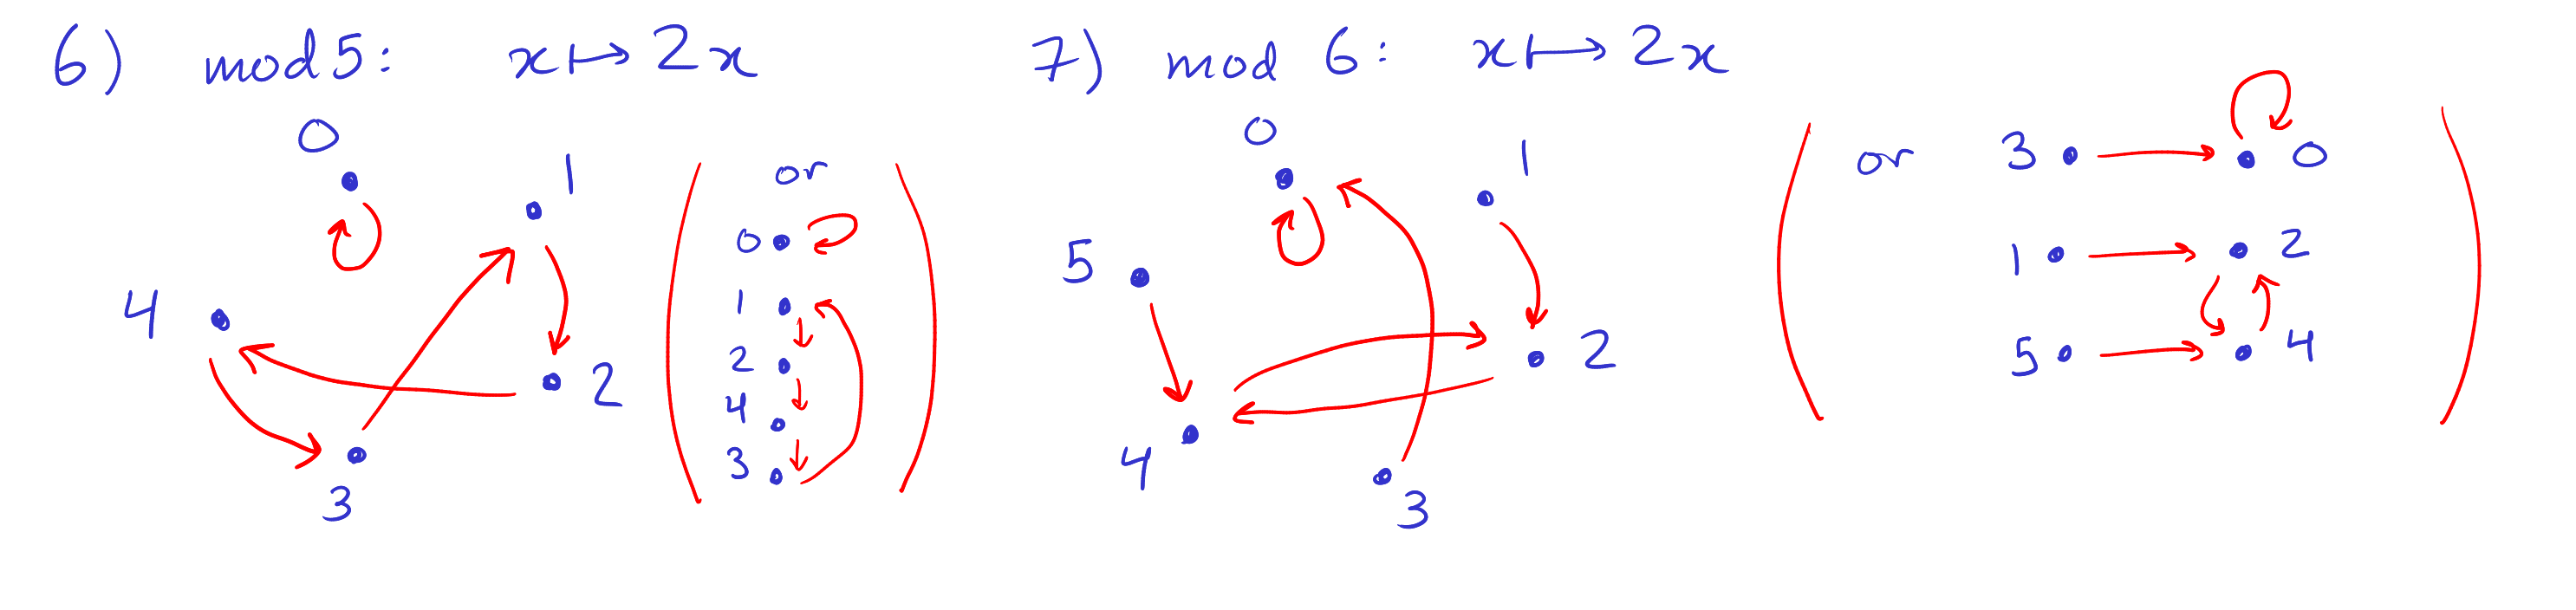
\includegraphics[width=0.9\textwidth]{mult-dyn-2-5-6.png}
\end{center}

In the diagrams above (called \textbf{dynamical portraits}), we can highlight the \textbf{orbit} of $1$, i.e. its future path by following arrows.  In the case of $5 \pmod 6$, $1$ is part of a cycle (it is \textbf{periodic}), because $x \mapsto 5x$ is bijective, and so a permutation, which falls into cycles.

However, in $2 \pmod 6$, $1$ is \textbf{strictly preperiodic}, meaning that it travels some distance before joining a cycle.


\subsubsection{Multiplicative order}

\begin{definition}
  Let $a \in \ZZ/n\ZZ$.  The \textbf{multiplicative order of $a$} is the smallest positive integer $k$ such that $a^k \equiv 1 \pmod n$, if it exists.
\end{definition}

For example:
\begin{enumerate}
\item $5$ has order $2$ modulo $6$.
\item $2$ has no order modulo $6$.
\item $1$ has order $1$ for all moduli (mod $n$ for all $n$).
\end{enumerate}

\begin{proposition}
Let $a \in \ZZ/n\ZZ$.  Then $a$ has a multiplicative order if and only if $a$ is invertible.
\end{proposition}

\begin{proof}
If $a$ has order $k$, then
\[
a^{k-1} a \equiv 1 \pmod n
\]
so $a$ is invertible (because its inverse is $a^{k-1}$).

Conversely, suppose that $a$ is invertible.  Then the sequence
\[
a, a^2, a^3, a^4, \ldots
\]
takes values in $\ZZ/n\ZZ$, a finite set.  So by the pigeonhole principle, 
\[
a^i \equiv a^j \pmod n
\]
for some $i < j$.  Since $a$ is invertible, we obtain
\[
1 \equiv (a^{-1})^i a^i \equiv (a^{-1})^i a^j \pmod n.
\]
Therefore, $a^{j-i} \equiv 1 \pmod n$.  Therefore $a$ has multiplicative order $j-i$ (which is positive by assumption).
\end{proof}

\subsubsection{The theorems of Euler and Fermat}

We can collect some data about orders:
\\

\begin{tabular}{lll}
modulus & possible orders & $\varphi(n)$ \\
\hline
2 & 1 & 1 \\
3 & 1,2 & 2 \\
4 & 1,2 & 2 \\
5 & 1,2,4 & 4 \\
6 & 1,2 & 2 \\
7 & 1,2,3,6 & 6 \\
8 & 1,2 & 4 \\
9 & 1,2,3,6 & 6 \\
10 & 1,2,4 & 4 \\
11 & 1,2,5,10 & 10
\end{tabular}

We observe that the orders all seem to divide $\varphi(n)$.  This is the substance of the next theorem:

\begin{theorem}[Euler's Theorem]
Let $a \in (\ZZ/n\ZZ)^*$.  Then
\[
a^{\varphi(n)} \equiv 1 \pmod n.
\]
\end{theorem}

\begin{proof}
The map $x \mapsto ax$ is bijective.  So it reorders the elements of $(\ZZ/n\ZZ)^*$.  Hence the product of all elements can be written two ways:
\[
\prod_{x \in (\ZZ/n\ZZ)^*} x
\equiv
\prod_{x \in (\ZZ/n\ZZ)^*} ax \pmod n.
\]
However, the two sides differ by the factor $a^{\varphi(n)}$.  Therefore, cancelling the product itself,
\[
a^{\varphi(n)} \equiv 1 \pmod n.
\]
\end{proof}

\begin{checkin}
% AI-FLAGGED ORIGINAL:
%    Observe that $\varphi(17)=6$ and $7^6 \equiv 7 \pmod{14}$.
    Observe that $\varphi(14)=6$ and $7^6 \equiv 7 \pmod{14}$.
\KS{Fixed by AI: the modulus here is $14$, and $\varphi(14)=6$ (whereas $\varphi(17)=16$). The footnote answer also refers to modulus $14$, so this should read $\varphi(14)=6$.}  This seems to contradict Euler's Theorem.  Why doesn't it?\footnote{Answer:  Euler's Theorem requires that the base, $a$, be in the multiplicative group.  But $a=7$ is not coprime to $14$, so Euler's Theorem doesn't apply to this base.}
\end{checkin}
\begin{aisolution}
Euler's Theorem only applies to bases $a \in (\ZZ/n\ZZ)^*$, i.e. bases coprime to $n$.  Here $\gcd(7,14) = 7 \neq 1$, so $7 \notin (\ZZ/14\ZZ)^*$ and the theorem simply does not apply.  (Indeed $7^2 = 49 \equiv 7 \pmod{14}$, so $7^k \equiv 7 \pmod{14}$ for every $k\geq 1$; the powers of $7$ never reach $1$.)
\end{aisolution}

The version of Euler's Theorem when $n$ is a prime is so important it is given a special name.

\begin{theorem}[Fermat's Little Theorem]
Let $p$ be prime.
Let $a \in (\ZZ/p\ZZ)^*$.  Then
\[
a^{p-1} \equiv 1 \pmod p.
\]
\end{theorem}

In particular, we learn that

\begin{corollary}
The order of any element $a \in (\ZZ/n\ZZ)^*$ is a divisor of $\varphi(n)$.
\end{corollary}

\begin{proof}
Currently a daily post question.
%Let $m$ denote the order.  Suppose $\varphi(n) \equiv t \pmod m$ for some $0 \le t < m$.  Then, $\varphi(n) + km = t$ for some integer $k$, so
%\[
%a^{t} \equiv a^{\varphi(n) + km} \equiv a^{\varphi(n)} (a^m)^k  \equiv 1 \cdot 1^k \equiv 1 \pmod n.
%\]
%By the definition of order, $m$ is the smallest positive integer so that $a^m \equiv 1$.  Therefore $t = 0$, and $\varphi(n) \equiv 0 \pmod n$, i.e. $m$ divides $\varphi(n)$.
\end{proof}

\subsubsection{Using Euler's $\varphi$ function}

\begin{example}
    

The question is to simplify
\[
	13^{453^{2022}} \pmod{100}
\]
by hand.

We wish to simplify the exponent $453^{2022}$ which lives modulo $\varphi(100)=40$.  This can be done since $13$ is coprime to $100$.

To compute $453^{2022} \equiv 13^{2022} \pmod{40}$, we can simplify the exponent modulo $\varphi(40)=16$ (this can be done since $13$ is coprime to $40$).  Reducing the exponent $2022$ modulo $16$ gets us
\[
	13^{2022} \equiv 13^6 \pmod{40}.
\]
We will need to do a little successive squaring or similar creativity to compute this.
\begin{align*}
	13^2 &\equiv 169 \equiv 9 \pmod{40}, \quad \\
	13^3 &\equiv 13 \cdot 9 \equiv 117 \equiv 37 \equiv -3 \pmod{40}, \quad \\
	13^6 &\equiv (13^3)^2 \equiv (-3)^2 \equiv 9 \pmod{40}.
\end{align*}
So we have discovered that
\[
	13^{2022} \equiv 9 \pmod{40}.
\]

Returning to the main problem, we now have reduced it to:
\[
	13^{453^{2022}} \equiv 13^9 \pmod{100}.
\]
To simplify $13^9$, we can use successive squaring:
\begin{align*}
	13^2 &\equiv 169 \equiv 69 \pmod{100}, \quad \\
	13^4 &\equiv 69^2 \equiv (-31)^2 \equiv 961 \equiv 61 \pmod{100}, \quad \\
	13^8 &\equiv 61^2 \equiv (-39)^2 \equiv 1521 \equiv 21 \pmod{100}, \quad \\
	13^9 &\equiv 13^8 \cdot 13 \equiv 21 \cdot 13 \equiv 273 \equiv 73 \pmod{100}.
\end{align*}

\end{example}



\subsubsection{Primitive roots}

\subsubsection{Summary of multiplicative structure in $\ZZ/n\ZZ$}




\subsection{Diffie-Hellman key exchange}

     {\bf Setup:}  $p$ (modulus), $g$
     \vspace{1em}

     \begin{tabular}{ccc}
       Alice & & Bob \\
       \hline
       Secret: $a$ & &  Secret: $b$ \\
       $g^a$ & $\longrightarrow$ & $g^a$ \\
       $g^b$ & $\longleftarrow$ & $g^b$ \\
       Compute: $(g^b)^a \equiv g^{ab}$ & & Compute: $(g^a)^b \equiv g^{ab}$
      \end{tabular}
      \vspace{3em}
      
      An eavesdropper Eve can see $g^a$ and $g^b$ and must compute $g^{ab}$.


      
\subsection{Efficient arithmetic modulo $n$ (a first introduction to complexity)}

\subsubsection{The role of modular exponentiation}

With Diffie-Hellman key exchange, we now have a working example of a key exchange cryptosystem.  Two things are needed from a practical key exchange:

\begin{enumerate}
    \item We need it to be \textbf{efficient} (fast) to \textbf{implement} the key exchange (in practice, a user is waiting for a browser to connect to a server).
    \item We need it to be \textbf{inefficient} (slow) to \textbf{break} the cryptographic scheme as an eavesdropper or attacker (in practice, an internet router listening to the conversation can't practically break the system).
\end{enumerate}

For the first, the computation of $g^a$ and $g^b$ modulo $p$ needs to be fast.  For the second, finding $g^{ab}$ from $g^a$ and $g^b$ has to be slow.  

We begin with the second of these conditions.  The na\"ive starting point is to make $p$ large enough so that the problem cannot be solved using exhaustive search.  That is, so that trying all possible values of $a$ and $b$ will take too long.  That means $p$ should be very big (since there are around $p$ possible $a$'s and $p$ possible $b$'s).  In practice, we may take $p$ to be around, say, $1024$ bits.

At that size, the exponent $a$ and $b$, chosen randomly in the range $0, \ldots, p-1$, can take on around $p$ different values and on average will be of size $p/2$.  That's still too big to count to.  So we cannot compute $g^a$ by repeatedly multiplying by $g$ a total of $a-1$ times.  For this to be a feasible system, we must compute it much much more efficiently than that.

\subsubsection{Successive squaring}

So how do we do modular exponentiation quickly?

Here's a puzzle to get you started:  try to compute $3^{32}$ modulo $n$, using as few multiplications as possible.  I've intentionally not given you the modulus, so you can't do this explicitly, but you can imagine yourself as a robot or computer program, which has two functions:  (1) multiplying two numbers to get a reduced result, and (2) storing results in memory.  For example, you might begin by computing $3$ times $3$ and storing the output $3^2$.  Then you might compute $3^2$ times $3^2$ and store $3^4$.

\begin{checkin}
        How many multiplications do you need to do, to compute $3^{32}$?
\end{checkin}
\begin{aisolution}
Five.  Since $32 = 2^5$, we can reach $3^{32}$ purely by repeated squaring: compute $3^2$, then $3^4 = (3^2)^2$, then $3^8$, $3^{16}$, and finally $3^{32}$.  Each step squares the previous value, so this is exactly five calls to the multiply subroutine.
\end{aisolution}


One clever approach is to repeatedly square.  That is, compute, in order:
\[
3^2, 3^4, 3^8, 3^{16}, 3^{32}.
\]
Each new value is a square of an existing value, so this requires calling the `multiply' subroutine exactly five times.

\begin{checkin}
    How many multiplications do you need to do, to compute $3^{36}$?
\end{checkin}
\begin{aisolution}
Six.  First build the successive squares $3^2, 3^4, 3^8, 3^{16}, 3^{32}$ (five multiplications).  Since $36 = 32 + 4$, one further multiplication $3^{32}\cdot 3^4 = 3^{36}$ finishes the job, for six in total.
\end{aisolution}

In this example, you might compute the same list as for the previous example, and then do one more multiplication:
\[
3^4 \cdot 3^{32} = 3^{36}.
\]

\begin{checkin}
    How many multiplications do you need to do, to compute $3^{39}$?
\end{checkin}
\begin{aisolution}
Eight.  The same five squarings produce $3^2, 3^4, 3^8, 3^{16}, 3^{32}$.  Since $39 = 32 + 4 + 2 + 1$, we then form $3^{32}\cdot 3^4 \cdot 3^2 \cdot 3 = 3^{39}$; combining these four factors takes three more multiplications.  The total is $5 + 3 = 8$.
\end{aisolution}

We might observe that
\[
39 = 32 + 4 + 2 + 1
\]
and thereby compute, using values from our list of successive squares,
\[
3^{32} \cdot 3^{4} \cdot 3^2 \cdot 3 = 3^{39}.
\]

\begin{checkin}
    How many multiplications did this last example take?\footnote{Answer:  5 to obtain a list of squares, then 3 more to put the appropriate squares together.}
\end{checkin}
\begin{aisolution}
Eight in total: the five squarings to build the list $3^2, 3^4, 3^8, 3^{16}, 3^{32}$, followed by three more to combine the four needed powers $3^{32}\cdot 3^4 \cdot 3^2 \cdot 3$ (combining $k$ factors takes $k-1$ multiplications, here $4-1 = 3$).
\end{aisolution}

This is called the method of successive squares.  To summarize:
\begin{enumerate}
    \item Write the exponent as a sum of powers of two, i.e. compute the binary expansion of the exponent.
    \item Create a list of successive squares that is large enough to include all the powers of two that appear in the expansion.
    \item Combine the indicated powers of two together.
\end{enumerate}

\begin{checkin}
    What is the maximal number of multiplications that this method may require to compute a power to an exponent $e$?
\end{checkin}
\begin{aisolution}
At most $2\lfloor \log_2 e\rfloor - 1$ multiplications.  The largest power of two we need is $2^{\lfloor \log_2 e\rfloor}$, so the list of successive squares $3^2, 3^4, \ldots, 3^{2^{\lfloor \log_2 e\rfloor}}$ costs $\lfloor \log_2 e\rfloor$ multiplications to build.  Combining the squares picked out by the binary expansion of $e$ costs at most $\lfloor \log_2 e\rfloor - 1$ more (start from one of the squares and multiply in the others).  Hence the worst case is $2\lfloor \log_2 e\rfloor - 1$, which is exponentially smaller than $e$ itself---the key fact that makes fast modular exponentiation, and thus public-key cryptography, possible.
\end{aisolution}

To answer this question, we first observe that the highest power of two needed will be given by $\lfloor(\log_2(e))\rfloor$.  For example, $5 < \log_2(39) < 6$, since $2^5 = 32 < 39 < 64 = 2^6$.  So we need five powers.

For the second, we may need to include all the squares, that is, we may begin with one square and multiply in all the others, for a total of $\lfloor(\log_2(e))\rfloor - 1$ possible.  The max is therefore
\[
2\lfloor(\log_2(e))\rfloor - 1.
\]

The important thing to observe here is that $\log_2(e)$ is \textbf{much much smaller} than $e$.  This is the distinction that makes cryptography work!  

There is another, slightly more efficient method of using the binary expansion of $e$ to compute a large exponent.  It is called the method of \textbf{square and multiply}. \KS{add info on this}

We will now turn to complexity.



\subsection{Runtimes and Big-Oh notation}

\subsubsection{Big-Oh notation}

Since the security of public key cryptography is based on the assumption that certain computations will necessarily take a long time, it is important to have a mathematical formalism for runtimes.  For this, we introduce Big-Oh notation in order to compare functions.  Because functions are so complicated (they have values at infinitely many inputs), we ask for a comparison that concerns their eventual (asymptotic) behaviour.  In other words, we ask which function is biggest as $x \rightarrow \infty$.  However, we also want to ignore constant scaling factors.  Taking these two aspects into account, we obtain the following definition.

\begin{definition}
	Let $f: [0,\infty) \rightarrow \RR$ and $g:[0,\infty) \rightarrow \RR$ be functions such that $g$ is eventually positive (meaning, it is positive for all sufficiently large inputs).  We say that $f(x) = O(g(x))$ (out loud, `$f$ is big-Oh of $g$') if there are constants $C > 0$ and $M > 0$ such that $|f(x)| \le C g(x)$ for $x > M$.
\end{definition}

This definition is meant to capture the `eventual' relative behaviour of $f$ and $g$, up to constant scaling factors.  That is, we would like to ignore constant scaling factors, and compare $f$ and $g$ only in the `tail' (as $x \rightarrow \infty$).  For an example, see Figure \KS{make a fig here showing $f = 100x^2$ and $g = x^3$ and how $f$ wins initially but $g$ wins eventually}.  We should think of $f = O(g)$ as saying that $f$ is bounded above by $g$ in a particular way (honestly, it's poor but very standard notation:  it's more like an inequality than an equality).

Here are some examples you should verify yourself:
\begin{enumerate}
	\item $x^2 + 3 = O(x^2)$
	\item $300x^2 = O(x^2)$
	\item $x^2 = O(x^3)$
\end{enumerate}

Here are some useful exercises (you can use the tool on my website).  For each pair of functions, determine if $f = O(g)$, $g = O(f)$ or both or neither.
\begin{enumerate}
	\item $f(x) = 500 \log (x)$ and $g(x) = x$
	\item $f(x) = |\sin(x)|$ and $g(x) = |\cos(x)|$
	\item $f(x) = |\sin(x)|$ and $g(x) = 1/2$.
\end{enumerate}

Example with solutions. 

For each of the following functions, determine if $f = O(g)$ and if $g = O(f)$ (it could be one, both or neither).

\begin{enumerate}
	\item $f(x) = |\sin(x)|$ and $g(x) = 1/2$.  The question whether $f = O(g)$ is whether we can choose an $M$ and a $C$ in the definition of Big-Oh so that $g$ `wins.'  Since both functions are periodic, taking a larger $M$ will not help matters.  So it comes down to $C$ in this case.  Since $f(x) = 0$ infinitely often, taking $C f(x)$ will never result in a function that is always greater than $1/2$.  Therefore $g \neq O(f)$.  On the other hand, taking $C = 2.1$ will guarantee that $C g(x) > f(x)$ always.  So $f = O(g)$.
	\item $f(x) = 2^x$ and $g(x) = 3^x$.  In this case, $g(x) > f(x)$ for all $x > 0$ so $f = O(g)$ certainly.  Does it work the other way?  In other words, can we choose a constant $C$ so that $3^x < C 2^x$ for sufficiently large $x$?  Well, $C = 3^c$ for some $c$, so cancelling $C$, we are asking about $3^{x-c} < 2^x$, or, rearranging, $e^{(x-c)\log(3)} < e^{x \log(2)}$, or, simplifying again, $(x-c)\log(3) < x \log (2)$.  At this point, we are comparing two linear functions.  Can we choose $c$ so that the right side is always bigger?  No, because the slope on the right side is smaller.  So $g \neq O(f)$.
\end{enumerate}

\subsubsection{Time and space complexity (runtimes)}

We want to measure an algorithm's \textbf{time complexity} (or \textbf{runtime}) in terms of the number of operations it takes to complete the algorithm, as a function of input size.  Similarly, we want to measure an algorithm's \textbf{space complexity} in terms of the number of bits of memory used, as a function of input size.

For example, consider the algorithm which takes as input an integer $n$, written in decimal notation, and prints ``Hello!'' exactly $n$ times.  The runtime is $n$ steps, each of which is a constant\footnote{I'm ignoring the intricacies of the counter itself} number of operations (printing the text and incrementing a counter that will determine when to stop).  So the runtime is $O(n)$ operations.  However, the input is of size $M := \log_{10}(n)$.  So, the runtime as a function of the input size $M$ is actually $O(n) = O(10^M)$ steps.  Thus, this algorithm is an \emph{exponential function} of the input size $M$.

As another example, trial division for factoring an integer $n$ tests at most $\sqrt{n}$ integers, so its runtime is $O(\sqrt{n}) = O(10^{M/2})$, again exponential.

We can divide runtimes we will encounter into three broad categories:
\begin{enumerate}
	\item \textbf{polynomial}:  $O(p(M))$ for some polynomial $p$ in the input size $M$.
	\item \textbf{exponential}:  $O(e^{p(M)})$ for some polynomial $p$ in the input size $M$.
	\item \textbf{subexponential}:  runtime less than $e^{p(M)}$ for all polynomials $p$.
\end{enumerate}

The last class lies between polynomial and exponential:  It is faster than any exponential function, but not necessarily polynomial.  Typically, we will see subexponential runtimes of the form $O( e^{c \sqrt{M \log M}})$ for some constant $c$.  Another example is $M^{\log M} = e^{(\log M)^2}$.  Both of these examples fail to be polynomial, but run faster than any exponential runtime.

Now let's consider the example of modular exponentiation using successive squaring.

Input:  a base $g$, an exponent $e$ and a modulus $n$, all written in decimal notation.  Thus the size of the input is $M = O(\log n)$.

Steps:  $log(n)$ squarings to create a list of successive squares, followed by at most $\log(n)$ multiplications to put the correct squares together according to the binary expansion.  Thus the runtime is $O(\log(n)) = O(M)$.

Thus the runtime is a polynomial (in fact, linear) number of multiplications.  How hard is a multiplication?  It is polynomial time (there are a lot of algorithms for this, some better than the schoolbook algorithm from grade school, but even that by-hand algorithm works digit-by-digit and is polynomial time.

So, overall, the runtime of modular exponentiation is polynomial time.  I have a computer demo for this (`Runtimes') on the cryptography website.

\subsection{The Discrete Logarithm}

When working in the multiplicative group $(\ZZ/n\ZZ)^*$ will use the notation $L_g(h)$ for the exponent to which one must raise $g \in (\ZZ/n\ZZ)^*$ to get the value $h \in (\ZZ/n\ZZ)^*$.  This is called the \textbf{discrete logarithm of $h$ to the base $g$}.  In other words, $L_g(h) = x$ if and only if $g^x \equiv h \pmod n$.  If no power of $g$ gives $h$, then this is not defined.

Note that $L_g(h)$ lives naturally in the ring $\ZZ/\varphi(n)\ZZ$, because it is an exponent.  For this reason, it is good to avoid asking for `$L_g(h)$ modulo $n$' but instead say `$L_g(h)$ working in $(\ZZ/n\ZZ)^*$' to be completely clear.  The word logarithm refers to an exponent.  Beyond this analogy, \textbf{this is not the logarithm you encounter in calculus}.  It will never be a decimal, for example!

\begin{checkin}
    What is $L_2(3)$ working in $(\ZZ/13\ZZ)^*$?  \footnote{Answer: This is a small enough ring to try some small Sage for loops or other experimentation.  Noticing that $2^4 \equiv 3 \pmod{13}$, we discover that $L_2(3) = 4$.}
\end{checkin}
\begin{aisolution}
List the powers of $2$ modulo $13$: $2^1 \equiv 2$, $2^2 \equiv 4$, $2^3 \equiv 8$, $2^4 \equiv 16 \equiv 3$.  Since $2^4 \equiv 3 \pmod{13}$, we have $L_2(3) = 4$.
\end{aisolution}

\KS{todo: pick other numbers in this checkin}
\begin{checkin}
    It is a fact that $p=101$ is prime, and $2$ is a primitive root modulo $p$.  It is a fact that $L_2(3)=69$ and $L_2(5)=24$ working in $(\ZZ/p\ZZ)^*)$.   It is also a fact that the integer factorization of $24$ is $24 = 2^3 \cdot 3$.  Using these facts, evaluate $L_2(24)$ working in $(\ZZ/p\ZZ)^*$ with minimal work (just combine the facts above).\footnote{Answer: From the factorization of $24$, we have $L_2(24) = 3 \cdot L_2(2) + L_2(3) = 3 \cdot 1 + 69 = 72$.  The log of $5$ is not needed.}
\end{checkin}
\begin{aisolution}
Discrete logs turn products into sums (of exponents, working modulo $p-1 = 100$).  Since $24 = 2^3\cdot 3$,
\[
L_2(24) = 3\,L_2(2) + L_2(3) = 3\cdot 1 + 69 = 72,
\]
using $L_2(2) = 1$ (as $2^1 = 2$) and the given $L_2(3) = 69$.  The value $L_2(5)$ is not needed.  (Check: $2^{72} \equiv 24 \pmod{101}$.)
\end{aisolution}



\subsection{The Discrete Logarithm Problem}

The security of the Diffie-Hellman Key Exchange relies on Eve not being able to discern the key from the public information.  This can be encapsulated as a hard problem in the following way:

\begin{problem}[The Computational Diffie-Hellman Problem (CDHP)]
	Given a prime $p$, a primitive root $g$, and the values $g^a$ and $g^b$ modulo $p$, find $g^{ab} \pmod p$.
\end{problem}

One way to solve the CDHP would be to figure out $a$ and $b$ and then compute $g^{ab}$.  We believe this is essentially the \emph{only} way to solve CDHP, but do not have a proof of that fact.  The problem of computing $a$ or $b$ is an example of the following problem.

\begin{problem}[The Discrete Logarithm Problem (DLP)]
	Given a prime $p$, a primitive root $g$, and the values $h = g^a$ modulo $p$, find $a$ modulo $p-1$.
\end{problem}

Notice that the exponent lives modulo $p-1$, so we can't really ask for $a$ more specifically than that (if $a$ works, then so does $a + p-1$).  We often assume we are looking for the smallest positive $a$, i.e. $0 \le a < p-1$.

The CDHP and DLP are believed to be equivalent, but this is only known in certain special cases.  It was shown by den Boer that there is a reduction when $\varphi(p-1)$ is smooth (\emph{smooth} means it is divisible by only fairly small primes), and this method was extended by Maurer to the situation where there is an efficiently constructible elliptic curve of smooth order over $\FF_q$ for each $q$ dividing $p-1$.  For recent progress on a quantum analogue, see Galbraith-Panny-Smith-Vercauteren. \KS{add proper citations}

The DLP has therefore been the focus of cryptanalytic attacks on Diffie-Hellman Key Exchange.

\subsection{Parity of discrete log}

\begin{question}
This exercise shows that the parity (even or oddness) of the discrete log in $(\ZZ/p\ZZ)^*$, $p$ an odd prime, can be discovered easily.
\begin{enumerate}
    \item Let $p$ be an odd prime number.
Show that if $ab \equiv 0 \pmod p$ then $a \equiv 0 \pmod p$ or $b \equiv 0 \pmod p$
\item Use part (1) on the expression $(x+1)(x-1)$ to show that the only two solutions to $x^2 \equiv 1 \pmod p$ are $1$ and $-1$.
\item Let $g$ be a primitive root mod $p$. Show that $g^{(p-1)/2} \equiv -1 \pmod p$.  (This uses the previous part.)
\item 
Suppose $h \equiv g^x \pmod p$ is given to you (but $x$ is not known).
Show how you can determine if $x$ is even or odd.
 Hint: Raise the equation $h\equiv g^x \pmod p$ to the $(p-1)/2$ power and see what you get using the previous part.

\item Note that $2$ is a primitive root modulo $11$. Use the test above to determine if $x$ so that $2^x \equiv 5 \pmod{11}$ is even or odd.
Check whether you are correct by finding $x$ (by any method).
\item Comment on the runtime of this test for the parity of $x$.
\item Comment on whether parity of a discrete log is well-defined modulo $n$.
\item Why is it ok for odd primes $p$?
\end{enumerate}
\end{question}
\begin{aisolution}
\begin{enumerate}
\item Suppose $ab \equiv 0 \pmod p$, so $p \mid ab$.  Since $p$ is prime, if $p \nmid a$ then $\gcd(p,a) = 1$, and multiplying $ab \equiv 0$ by $a^{-1}$ modulo $p$ gives $b \equiv 0 \pmod p$.  Hence $a \equiv 0$ or $b \equiv 0 \pmod p$.  (This is Euclid's Lemma.)
\item If $x^2 \equiv 1 \pmod p$ then $(x+1)(x-1) = x^2 - 1 \equiv 0 \pmod p$.  By part (1), either $x+1 \equiv 0$ or $x-1 \equiv 0$, i.e. $x \equiv -1$ or $x \equiv 1 \pmod p$.  So the only solutions are $\pm 1$.
\item Let $y = g^{(p-1)/2}$.  Then $y^2 = g^{p-1} \equiv 1 \pmod p$ by Fermat's Little Theorem, so by part (2), $y \equiv \pm 1$.  If $y \equiv 1$, then $g^{(p-1)/2} \equiv 1$ would make the order of $g$ at most $(p-1)/2 < p-1$, contradicting that $g$ is a primitive root (order exactly $p-1$).  Hence $g^{(p-1)/2} \equiv -1 \pmod p$.
\item Raise $h \equiv g^x$ to the power $(p-1)/2$:
\[
h^{(p-1)/2} \equiv \left( g^{(p-1)/2} \right)^x \equiv (-1)^x \pmod p,
\]
using part (3).  Thus $h^{(p-1)/2} \equiv 1 \pmod p$ if $x$ is even, and $\equiv -1 \pmod p$ if $x$ is odd.  Computing $h^{(p-1)/2} \bmod p$ therefore reveals the parity of $x$.
\item Here $p = 11$, so $(p-1)/2 = 5$, and $h = 5$.  We compute $5^5 \pmod{11}$: $5^2 \equiv 3$, $5^4 \equiv 3^2 \equiv 9$, $5^5 \equiv 9\cdot 5 \equiv 45 \equiv 1 \pmod{11}$.  Since the result is $+1$, $x$ is \emph{even}.  Checking directly: the powers of $2$ modulo $11$ are $2,4,8,5,\ldots$, so $2^4 \equiv 5 \pmod{11}$, giving $x = 4$, which is indeed even.
\item The test is a single modular exponentiation $h^{(p-1)/2} \bmod p$, computable by successive squaring in $O(\log p)$ multiplications---polynomial in the input size.  So parity is \emph{easy} to determine, even though computing $x$ itself (the full discrete log) is believed to be hard.
\item The discrete log $x$ is only defined modulo the order of $g$ (here $p-1$): replacing $x$ by $x + (p-1)$ gives the same $h$.  So parity is well-defined only when this ambiguity preserves parity, i.e. when the order is even.  In general, working modulo $n$, the log lives modulo $\mathrm{ord}(g)$, and its parity is well-defined precisely when $\mathrm{ord}(g)$ is even.
\item For an odd prime $p$, the modulus of the exponent is $p-1$, which is even.  Adding an even number never changes parity, so the parity of $x$ is well-defined; moreover parts (2)--(3) require $p$ to be an odd prime (so that $1 \neq -1$ modulo $p$ and Euclid's Lemma applies).
\end{enumerate}
\end{aisolution}

\begin{solution}
    \begin{enumerate}
        \item Suppose $ab \equiv 0 \pmod{p}$.  Then $p \mid ab$.  By the primality of $p$, this implies either $p \mid a$ or $p\mid b$.  Thus $a \equiv 0 \pmod{p}$ or $b \equiv 0 \pmod{p}$.
        \item Rewrite $x^2 \equiv 1 \pmod{p}$ as $(x+1)(x-1)$ modulo $p$ and then apply the last part with $a = x+1$ and $b=x-1$.  We discover that either $x \equiv 1$ or $x \equiv -1$.
        \item We know that $g^{p-1} \equiv 1 \pmod{p}$ from Fermat's little theorem.  If $g$ is primitive root, then $g^{(p-1)/2}$ is not $1$, but by the previous part, the only other possibility is $-1$.
        \item Raising the equation to power $(p-1)/2$, we discover that $h^{(p-1)/2} \equiv (-1)^x$.  Thus depending on whether $h^{(p-1)/2}$ is $1$ or $-1$ we can infer that $x$ is even or odd, respectively.
        \item Use $p=11$, $g=2$, $h=5$.  Try $h^{(p-1)/2}$ modulo $p$, which is $5^5 \pmod{11}$, which is $1$.  This implies that $x$ is even.  Running through the powers of $2$ manually we find that $2^4 \equiv 5 \pmod{11}$ so that $x = 4$.
        \item We need only do a modular exponentiation, which takes roughly $\log(p)$ steps.
        \item The discrete log is defined modulo $\varphi(n)$.   It is well-defined when $\varphi(n)$ is even.  This is because taking a different representative of the equivalence class modulo $\varphi(n)$ doesn't change whether it is even or odd.   This is the case for all odd primes $p$, since $\varphi(p) = p-1$, which is even.
    \end{enumerate}
\end{solution}


\subsubsection{The Baby-Step Giant-Step Algorithm}
\KS{AI: this is the section referenced elsewhere as \texttt{sec:baby-giant}, but it has no matching label, so that cross-reference renders as "LABEL:sec:baby-giant" in the EC El~Gamal section. Add \texttt{\textbackslash label\{sec:baby-giant\}} right here to fix it.}

The first algorithm we will study which is faster than exhaustive search for the Discrete Logarithm Problem is known as the \emph{Baby-Step-Giant-Step} algorithm, and is due to Shanks \KS{add citation}.  It is an example of a \emph{meet-in-the-middle} algorithm, because we compute two lists and look for a collision.  To motivate the algorithm, suppose we compute two lists of randomly generated elements of $\ZZ/p\ZZ$.  The first list consists of elements of the form $g^j$, i.e., random powers of the generator $g$.  The second list consists of elements of the form $hg^k$, i.e. random powers of $g$, all multiplied by $h$.  If we notice a collision, i.e. $g^j = h g^k$, then rearranging, we obtain $g^{j-k} = h$ and $j-k$ is the solution to the problem.  

Such an attack is sometimes called a \emph{birthday attack}.  It is an improvement over the more na\"ive method of computing a single list of random powers of $g$ and hoping to collide with $h$.  Indeed, the number of comparisons that may result in a collision in this na\"ive method is equal to the length $\ell$ of the list.  But with two lists of length $\ell$, there are ${\ell\choose 2} = \frac{\ell(\ell-1)}{2}$\KS{Fixed by AI: the original wrote $\frac{\ell(\ell+1)}{2}$, but $\binom{\ell}{2}=\frac{\ell(\ell-1)}{2}$.} comparisons that may `get lucky.'  This results in an improved runtime, since we obtain more new comparisons per computation of an element.  (It does require more memory, however).

Shanks' Baby-Step-Giant-Step algorithm takes the randomness out of this two-list approach, by generating two lists which are expected to `cover' the space of possibilities fairly evenly.  To make this precise, start with the observation that every integer $0 \le n < 100$ can be written with two base-ten digits in a unique way.  Similarly, any integer $0 \le n < p-1$ can be written uniquely with two digits in base $\sqrt{p-1}$, or at least, approximately so, since if $\sqrt{p-1}$ is not an integer, we will use the closest integer greater than it.  That is, we let $N = \lceil \sqrt{p-1} \rceil$.\KS{Fixed by AI: the original ``$\rceil p-1 \lceil$'' had reversed ceiling brackets and, more importantly, omitted the square root; the base used is $\sqrt{p-1}$, so $N=\lceil\sqrt{p-1}\rceil$.}

The first list is the `baby steps':
\[
	g, g^2, g^3, g^4, g^5, \ldots
\]
The second list is the `giant steps':
\[
	h, hg^{-N}, hg^{-2N}, hg^{-3N}, \ldots
\]
We look for a collision, namely an element that appears in both lists:
\[
	g^j = hg^{-kN}
\]
Then, rearranging, we have
\[
	g^{j+kN} = h
\]
In other words, having found a collision, we see immediately that the solution (the exponent we seek) is $j+kN$.

\KS{Insert an example}

% >>> AI-GENERATED EXAMPLE (needs review) >>>
\begin{example}
Let us solve the discrete logarithm problem $2^x \equiv 5 \pmod{29}$, where $g = 2$ is a primitive root modulo the prime $p = 29$.  Here $p - 1 = 28$, so we set $N = \lceil \sqrt{28} \rceil = 6$.

\emph{Baby steps.}  We list $g^j = 2^j \pmod{29}$ for $j = 0, 1, \ldots, 5$:
\[
2^0 \equiv 1, \quad 2^1 \equiv 2, \quad 2^2 \equiv 4, \quad 2^3 \equiv 8, \quad 2^4 \equiv 16, \quad 2^5 \equiv 3 \pmod{29}.
\]

\emph{Giant steps.}  We list $h \cdot g^{-Nk} = 5 \cdot 2^{-6k} \pmod{29}$.  First we need $g^{-N} = 2^{-6} \pmod{29}$: since $2^6 \equiv 6$ and $6 \cdot 5 \equiv 30 \equiv 1 \pmod{29}$, we have $2^{-6} \equiv 5$.  Then, multiplying by $5$ at each step,
\[
k = 0:\ 5, \qquad k = 1:\ 25, \qquad k = 2:\ 9, \qquad k = 3:\ 16 \pmod{29}.
\]

\emph{Collision.}  The value $16$ appears in both lists: it is the baby step $g^4$ (with $j = 4$) and the giant step with $k = 3$.  Setting these equal,
\[
g^{4} \equiv h \cdot g^{-6 \cdot 3} \pmod{29}, \quad \text{so} \quad h \equiv g^{4 + 18} \equiv g^{22} \pmod{29}.
\]
Therefore $x = j + kN = 4 + 3 \cdot 6 = 22$.  Indeed, one checks that $2^{22} \equiv 5 \pmod{29}$.  Notice that we found the answer after computing only $6 + 4 = 10$ powers, rather than searching through all $28$ possible exponents.
\end{example}
% <<< END AI-GENERATED EXAMPLE <<<

\KS{Insert runtime analysis}

Other exponential methods include the Pollard $\rho$ and $\lambda$ methods.

\subsubsection{Pohlig-Hellman}

The importance of the Pohlig-Hellman algorithm is that it works efficiently when $p-1$ is \emph{smooth} (has only small prime factors).  The lesson to take away is that one should always choose $p$ so that $p-1$ does not have small factors.

\KS{complete this section}

\subsubsection{Index Calculus}

This method leverages linear algebra by changing the equation $h = g^x$ into the linear equation $L_g(h) = x$, and more generally, any multiplicative relation
\[
	h^ag^b = h^c g^d
\]
into a linear equation concerning the exponents
\[
	a L_g(h) + b = c L_g(h) + d.
\]
Such an equation can be solved in a linear fashion:
\[
	L_g(h) = \frac{d-b}{a-c}.
\]
If we can involve more variables, we can create larger linear systems of equations.   For example, if we happen to know that
\[
	gh^2 = 2 \cdot 3, \quad \text{and } h^3 = 3 \cdot 2^2 g
\]
then we obtain a system of linear equations in the unknowns $L_g(h)$, $L_g(3)$ and $L_g(2)$:
\[
	1 + 2 L_g(h) = L_g(2) + L_g(3), \quad 3 L_g(h) = L_g(3) + 2 L_g(2) + 1
\]
With enough relations, we can create a determined or over-determined system of linear equations.
This is the point of inspiration for the index calculus.

The algorithm has the following basic form:  first, we collect a large number of linear equations in a large number of variables; and second, solve the system.  We will actually do this twice.

In the first stage, called the \emph{precomputation}, we don't use the value of $h$ at all.  We will choose a list of primes $p_1, \ldots, p_m$ called the \emph{factor base}.  It is useful if they are small, so typically, this is chosen to be all primes below some bound $B$; we will make this assumption.  The discrete logarithms $L_g(p_1), \ldots, L_g(p_m)$ will be the variables in our linear system.

To generate some linear equations in these variables, we compute $g^k$ for random values of $k$, and hope that the smallest integer residue $g^k$ can be written as a product in terms of the primes $p_i$. For example, if $g^7 = 2^2 \cdot 3$, then we learn that $7 = 2 L_g(2) + L_g(3)$.  In general, if 
\[
	g^k = \prod_{i=1}^m p_i^{e_i},
\]
then we obtain an equation (called a \emph{relation})
\[
	k = \sum_{i=1}^m e_i L_g(p_i).
\]
With enough relations (at least $m$ of them), we hope to obtain a linear system with a unique solution.  We continue to generate relations until we have a unique solution.  We are doing linear algebra modulo $p-1$, i.e. in the ring $\ZZ/(p-1)\ZZ$.  With large systems, we need some formal methods.  For small systems it is easy to use high school methods (adding equations to one another) to solve small systems.  The advantage of this method is that linear algebra is fast in $\ZZ/(p-1)\ZZ$; for formal algorithms we will need to wait until we have the Chinese Remainder Theorem and other tools of modular arithmetic.

Solving the system, then, we have values for $L_g(p_i)$ for all $p_i$.  This completes the precomputation.

The second stage uses the value of $h$.  We look for at least one more relation, this time involving a new variable $L_g(h)$.  To find such a relation, compute $hg^k$ for random values of $k$, and hope that it can be written as a product in terms of the $p_i$.  If so, we have
\[
	hg^k = \prod_{i=1}^m p_i^{e_i},
\]
which translates into a linear equation
\[
	L_g(h) + k = \sum_{i=1}^m e_i L_g(p_i).
\]
Since we know the values of all the $L_g(p_i)$, this gives an equation for $L_g(h)$, the goal of the algorithm.

As an example, let $p=127$ and $g=3$.  For a factor base, let's choose primes less than $B = 20$:
\[
	2,3,5,7,11,13,17,19
\]
Now we can compute $g^k$ for some random values of $k$:
\begin{gather*}
	g^{37} \equiv 2^4\cdot 3, \quad
	g^{68} \equiv 11, \quad
	g^{4} \equiv 3^4, \quad
	g^{23} \equiv 83, \quad
	g^{31} \equiv 2 \cdot 3 \cdot 19, \quad 
	g^{40} \equiv 2 \cdot 13, \quad \\
	g^{98} \equiv 37, \quad
	g^{52} \equiv 2^3 \cdot 3 \cdot 5, \quad
	g^{61} \equiv 2 \cdot 7, \quad
	g^{10} \equiv 11^2, \quad
	g^{49} \equiv 3 \cdot 5^2, \quad
	g^{78} \equiv 61, \quad
	g^{73} \equiv 2 \cdot 3
\end{gather*}
These are all shown in factored form.  We don't need to factor them completely, we only need to find out how the factor base primes appear.  We have to throw out those which don't factor completely into the factor base.  The remaining values form a linear system modulo $p-1$:
\begin{align*}
	37 &\equiv 4 L_g(2) + L_g(3), \\
	68 &\equiv L_g(11), \\
	4 &\equiv 4 L_g(3), \\
	31 &\equiv L_g(2) + L_g(3) + L_g(19), \\
	40 &\equiv L_g(2) + L_g(13), \\
	52 &\equiv 3L_g(2) + L_g(3) + L_g(5), \\
	61 &\equiv L_g(2) + L_g(7), \\
	10 &\equiv 2L_g(11), \\
	49 &\equiv L_g(3) + 2L_g(5), \\
	73 &\equiv L_g(2) + L_g(3).
\end{align*}
We can solve this system using efficient computer linear algebra, but in this toy example, we can solve by hand\footnote{this may require inverting something modulo $p-1$; this is covered in later chapters but is efficient, meaning, polynomial time in the log of the modulus, providing the element is invertible}.  I'll show the steps here, to be clear.

Notice that since $g=3$, we already know $L_g(3) = 1$.  We can solve for $L_g(11)$ using the second equation.  So we have:
\begin{gather*}
	L_g(3) \equiv 1, \quad
	L_g(11) \equiv 68, \quad
\end{gather*}
Next, we can use the last equation to obtain $L_g(2)$ (note that we can't use the first equation, because it would involve cancelling a $4$ which is not allowed mod $126$):
\begin{gather*}
	L_g(2) \equiv 73 - 1 \equiv 72, \quad
\end{gather*}
From the 6th equation, we can solve for $L_g(5)$:
\begin{gather*}
	L_g(5) \equiv 52-3 \cdot 72- 1 \equiv -165 \equiv 87, \quad \\
\end{gather*}
The 7th equation gives $L_g(7)$, the 5th gives $L_g(13)$ and the 4th gives $L_g(19)$:
\begin{gather*}
	L_g(7) \equiv 61 - 72 \equiv 115, \quad
	L_g(13) \equiv 40 - 72 \equiv 94, \quad
	L_g(19) \equiv 31 - 72 - 1 \equiv 84.
\end{gather*}
This completes the precomputation phase.

Now we can move on to the second phase, where we use $h$.  Suppose $h=34$.  We try to factor $hg^k$ for some random $k$ and discover that
\[
	h\cdot g^{85} \equiv 3 \cdot 11.
\]
This linearizes to the relation
\[
	L_g(h) + 85 \equiv L_g(3) + L_g(11).
\]
Using the data from the precomputation, this becomes
\[
	L_g(h) \equiv 1 + 68 - 85 \equiv -16 \equiv \varphi(p) - 16 = 127 - 1 -16 \equiv 110.
\]
Notice that since the exponent lives modulo $\varphi(p)$, I can modify it to take on its smallest positive value.

Now, we confirm the computation by directly computing
\[
	g^{110} \equiv 3^{110} \equiv 34 \equiv h \pmod{127}.
\]
This confirms the answer.

If we want to compute another discrete log with the same $g$ and $p$, we need only repeat the second phase; all the precomputation is already useful.  For example, if we choose $h=71$, we find
\[
	L_g(h) + 29 = L_g(5) + L_g(19)
\]
which gives $L_g(h) = 87 + 84 - 29  = 16$. 

\subsubsection{Runtime}

This analysis will necessarily lack some details, as the full analysis is very complex.  
There are two modes to this algorithm:  finding relations, and linear algebra.  As it turns out, the linear algebra is not the bottleneck.  Therefore we will focus on the relation-finding phase, whose runtime is controlled by the bound $B$, which is referred to as the \textbf{smoothness bound}.  (A `smooth' number is one which has only small prime factors.)  Roughly speaking, if $B$ is larger, then we are more likely to find relations (the value $g^k$ is more likely to be written as a product of the primes in the factor base), but at the same time, factoring each $g^k$ in terms of the factor base is more work (recall that we only need to factor it partially, namely, we need only identify the part of the prime decomposition that consists of primes from the factor base). 

We begin with the probability that a random integer $0 \le n \le p-1$ can be factored completely in terms of the primes of the factor base (this is called being \textbf{$B$-smooth}).  This is a deep result of Canfield, Erd\"os and Pomerance, which says that under appropriate hypotheses, and changing variables so that
\[
	u = \frac{\log p}{\log B}, \quad B = p^{1/u},
\]
the probability is around $u^{-u}$. \KS{give proper citation}.  Thus, we expect that it will take around $u^u$ trial values $g^k$ before we find one that factors completely in the factor base.

We will assume that the factoring is done by trial division in terms of the factor base (in fact, there are various improvements that can be made).
The runtime for finding relations can then be expressed as a product:
\[
	(\text{\# of relations needed})(\text{average tries per success})(\text{\# of trial divisions to factor})(\text{cost of a trial division}).
\]
Write $\pi(B)$ for the number of primes in the factor base (i.e., the number of primes less than $B$).  Since there are $\pi(B)$ variables $L_g(p_1), \ldots, L_g(p_m)$ in the linear system, we need at least $\pi(B)$ equations to narrow the solution down exactly.  Then the expression above becomes
\[
	\pi(B) u^u \pi(B) \operatorname{poly}(\log p).
\]
Here, we are using the fact that trial division is a polynomial algorithm in the input.  Thus, we hope to minimize this quantity.  Ignoring the polynomial in $\log p$ and approximating $\pi(B)$ by $B$ (actually $\pi(B) \sim B/\log B$), we can simplify our quantity to the approximation
\[
	B^2 u^u = p^{2/u} u^u.
\]
To minimize this, we use standard methods of calculus:  we take the log of both sides:
\[
	\frac{2}{u} \log p + u \log u.
\]
Then, taking the derivative, we have
\[
	\frac{-2}{u^2} \log p + \frac{2}{up} \frac{dp}{du} + \log u + 1
\]
We want this to be $0$ to find minima.  We assume that the dominant terms are
\[
	\frac{-2}{u^2} \log p + \log u,
\]
and this should vanish when
\begin{equation}
	\label{eqn:up}
	u^2\log u = 2\log p.
\end{equation}
We can't solve for $u$ directly, but if we choose
\[
	u = 2\sqrt{ \frac{\log p}{\log \log p} }
\]
then we will get very close.  A graph is shown in \KS{add a graph}.  Using this, %Actually, as soon as we know there is a minimum, we can use \eqref{eqn:up} to compute
\[
	u \log u \sim \frac{2 \log p}{u} \sim \sqrt{ \log p \log \log p},
\]
and
\[
	B = p^{1/u} = e^{\frac{\log p}{u}} \sim e^{ \frac{1}{2} \sqrt{ \log p \log \log p}}.
\]
Thus,
\[
	B^2 u^2 \sim d^{\sqrt{\log p \log \log p}}.
\]
This is the runtime when $B$ is chosen to minimize runtime, and this is an example of a subexponential runtime.

There are a wide variety of improvements and variations on this algorithm, including others from the same family known as the \emph{number field sieve} and \emph{function field sieve}.  But they all have subexponential runtimes.  In fact, if we set the convenient notation
\[
	L_p(\alpha,c) = e^{(c+o(1)) (\log p)^\alpha (\log \log p)^{1-\alpha}}
\]
then this algorithm has runtime $L_p(1/2,1)$ and variants have runtimes $L_p(\alpha,c)$ for other values of $\alpha$ and $c$.



\subsubsection{Logjam attack}

Observe that most of the work in this algorithm lies in the precomputation phase.  This phase depends only on the prime and primitive root, not on the value of $h$.  This is also true of the \emph{number field sieve} and \emph{function field sieve}.  
This led to the famous \textbf{Logjam attack} \KS{give citation to webpage weakdh.org}, revealed publicly on May 20, 2015.  This attack consisted of two components.  The first was a weakness in the $TLS$ handshake protocol between client and server that allowed a \textbf{man-in-the-middle} (someone altering messages passing between client and server) to force the server to use a relatively weak (but still built-in) $512$-bit prime, even when server settings dictated the use of a stronger prime.  The second component was a large precomputation for the number field sieve for the most commonly used prime(s) $p$.  It turns out that some $8.4\%$ of the top 1 million websites were using this most popular prime number.  By running the precomputation offline before the attack, the online, active phase of the attack could be made very quick (a matter of around a minute).  The researchers who created and revealed the Logjam attack speculated that a nation state agency such as the National Security Agency may have the server power and money (in the hundreds of millions\KS{cite wikipedia or the original paper}) to run pre-computations for the most common $1024$-bit prime, obviating the need for the first component, and allowing them to decrypt a significant portion of internet traffic (around a quarter of websites and two thirds of VPNs).  The researchers released instructions to server administrators on how to avoid this attack.


\subsection{A lower bound on solving discrete log}

At this point in our discussion, I have emphasized several times that the only reason we have confidence in our cryptographic protocols is that many highly trained human beings have spent a lot of mental energy trying to come up with faster discrete log algorithms, and have failed to find anything faster than subexponential.  We can't provide a lower-bound on the runtime of discrete logarithm algorithms -- besides trivial ones, such as the time it takes to write down an answer.

However, if we are willing to limit the model we work in, we can provide a sort of lower bound, and that's what this section is about.  Let $g$ be a generator for the multiplicative group modulo $p$.  Recall that the security of the discrete logarithm relies on the fact that the names of the residues modulo $p$ don't seem to give us any information on where in the cycle of powers of $g$ the residues lie.  When I tell you I'm thinking about $147$ modulo $823$, that name -- `147' -- doesn't tell you what power of the generator $3$ it is.  Or so it seems.

But what if we could create a thought experiment in which we have an `ideal' group where the names of its elements really are truly inscrutable.  You could imagine modelling such a group by putting $(\ZZ/p\ZZ)^*$ behind a curtain and having Mr. Spock relabel all the residues totally randomly.  One is called `Joe' and another `Pickle' and another one is `Spongebob' and no one but Mr. Spock knows which is which.

Notice that in such a situation, you could still run the birthday attack.  You could ask for various powers of `Bob' and Mr. Spock would reveal their names, and you could store them in a list.  As long as Mr. Spock is consistent -- if $147$ is called `Pebbles', he doesn't change the name to `Dweezle' partway through the game -- then you can just watch for a collision.

So in this sense, the birthday attack is a totally general attack on a cyclic group.  It doesn't need to know anything about the elements except that they have a group law and a consistent naming convention.

Compare this to the index calculus.  If I tried to run the index calculus algorithm against Mr. Spock, I would ask for a power of `Bob', get back `Ahmed' and then attempt to do trial division on Ahmed, at which point Ahmed would probably get fed up and tell me to stop poking him with my slide rule.  I can't do trial division on an abstractly named group element.  I need to have a number.  So the index calculus is not a general algorithm.

This thought experiment can be turned into a formal proof that the best totally generic algorithm against the discrete logarithm problem runs in time $O(\sqrt{p})$ group operations.  The method of proof is a little wacky -- it basically involves setting up a thought experiment like this, with a \emph{simulator} like Mr. Spock -- except Mr. Spock doesn't actually know the answer to the discrete log problem either!  Amazingly, a little careful analysis of this game of  `the blind leading the blind' can give a lower bound.

Here's how it goes.  The group $(\ZZ/p\ZZ)^*$ is behind a curtain, and Mr. Spock is tasked with \emph{pretending}, as best he can, to have assigned silly but consistent names to its group elements.  The task for you is to solve the discrete logarithm problem which asks, which power of Gracie gives Helmut?  Mr. Spock doesn't actually \emph{know} which element of $(\ZZ/p\ZZ)^*$ is Gracie or Helmut, but he will pretend he does.  

Now for a twist.  In our game, the group $(\ZZ/p\ZZ)^*$ is a third player.  It has decided which residue is Gracie and which is Helmut, but it has only kept this information to itself in a manilla envelope, like the envelope containing Colonel Mustard with the Rope in the Kitchen at the beginning of the board game Clue\footnote{If you don't know this reference, Clue is a game in which the solution to a crime is hidden in an envelope at the beginning, and the players take turns finding some clues to narrow down the possibilities.}.

Mr. Spock, meanwhile, can't see in the envelope, but is pretending to `be' the group $(\ZZ/p\ZZ)^*$ as we discussed.

You will win this fever-dream-of-the-computer-scientist game if you can either (a) solve the discrete log problem; or (b) catch Mr. Spock in his lie.  The rules you must follow are that you can ask Mr. Spock to perform group operations (such as additions and multiplications or exponentiations) using the silly element names (which are all you ever get to see).  So for example, you could ask Mr. Spock to raise Gracie to the power ten.

Mr. Spock is going to play this game to the best of his ability, which means he is going to keep a table for himself of all the answers he has given before, and attempt to avoid contradicting himself.  However, he \emph{doesn't know the envelope-clad actual solution to the discrete log problem} so he could mess up anyway.

In particular, if in the manilla envelope, the group has decided that in fact Gracie to the tenth power is Helmut, then, Spock should answer Helmut when you ask for Gracie to the power ten.  But Mr. Spock, ignorant of the true answer to the discrete log problem in the envelope, will simply make up a new silly name for this computation's result.

Now, so far the group isn't playing the game at all.  It's hidden something in an envelope and we can't see that anyway, so it might as well be in another country.  But for one fact:  if Mr. Spock messes up and `lies', giving an answer that contradicts the answer in the envelope, then the group will immediately call an end to the game and declare you the winner!

Assuming this doesn't happen, after some number of queries to Mr. Spock, you will guess the discrete log answer.  How well can you do?

The key to this thought experiment is that the group, besides having chosen the correct answer, \emph{isn't participating in the game (except possibly to suddenly end it)}, so the correct answer isn't available either to you or to Mr. Spock during the game's duration.  So, by information theory, you really don't stand a chance to discover the discrete logarithm.

The only real way you can hope to win the game is by tripping up Mr. Spock, triggering the group to end it.  And to do that, you need to make enough queries to him that he will, statistically, eventually say something contradicting the hidden envelope.

Having laid out the general plan, what remains is to formalize the probabilities.  We will now give the formal proof.

\begin{theorem}
    Assuming Mr. Spock plays well, you cannot devise an algorithm that wins this game with non-negligible probability in fewer than $O(\sqrt{p})$ queries to Mr. Spock.
    \end{theorem}

    \begin{proof}
Mr. Spock plays the game as follows.  He keeps a list of your requests (which are all combinations of Gracie and Helmut, since you have no other elements to begin with). If you ask for $G^a H^b$ (where $G$ stands for Gracie and $H$ for Helmut), he stores this as $a + bx$ and assigns it a random silly name, which he also stores.  Every time you ask for an element, checks if it is in his list, and if not, adds it and makes up a new name.  Otherwise he responds with the existing name from the list.
    
    Now go ahead, imagine your best algorithm.  Using that algorithm, make $N$ queries to Mr. Spock (the \emph{simulator} in CS terminology).  Then guess the answer, the hidden discrete logarithm, say $z$.  Let's call the actual answer in the envelope $y$, so $G^y = H$ in reality (in the group).
    
    What's the probability that you won by tripping up Mr. Spock?  If plugging in $y$ for $x$ results in two of the polynomials in his list becoming the same number, then he has lied, giving two different names to the same group element, and you win.  This is the only way he could be tripped up.  Given that $y$ is essentially random from the perspective of you and Mr. Spock, the probability that this happened is the probability that $a_i + b_i x = a_j + b_j x$ for some $i \neq j$.  In Mr. Spock's list there are at most $N$ entries (assuming you didn't ask many redundant queries), so $N$ choose $2$ pairs $(i,j)$ to check.  Each equation is of the form $(b_j-b_i)x = (a_i-a_j)$, which has at most one solution (since $i \neq j$), so a probability of at most $1/(p-1)$ of triggering Mr. Spock's demise.  So the probability that Mr. Spock is caught out is ${{N}\choose{2}} \frac{1}{p-1} = O(N^2/p)$.  In other words, there are about $O(N^2)$ values of $y$ that, if they were in the envelope, would have caused Mr. Spock to be caught.

    What's the probability that you won by guessing the correct discrete logarithm?  The only information you could possibly have in this case is that you didn't trigger Mr. Spock's demise, which rules out at most $O(N^2)$ values of $y$, as we have seen.  So you can choose from the remaining $M := p-1 - {{N}\choose{2}}$ possible values, if you are your smartest self (i.e. in the best case algorithm scenario).  So the probability that you won this way is the probability that Mr. Spock was not caught out, times the probability you guessed correctly, i.e. (in the order just given),
    \[
    \frac{M}{p-1} \cdot \frac{1}{M} = \frac{1}{p-1}.
    \]
    So your best bet is to hope Mr. Spock is caught, and that happens with, at best, probability $O(N^2/p)$.  So for a good chance at winning this game, you need to make about $\sqrt{N}$ queries.
\end{proof}

What remains is to interpret the result as saying \emph{the best generic group algorithm requires at least $O(\sqrt{p})$ group operations}.  The idea here is that a generic algorithm is one which can do group operations, but can't use anything about the group element names or any other information about the group.  Then the key is that \emph{if there's a good such algorithm, then it would perform well against Mr. Spock in the game above}.  That is, a generic algorithm in this sense could be used with Mr. Spock since it doesn't require anything other than group operations.  The fact that Mr. Spock can get caught out and end the game early is an annoyance, but you can just assume you would have won in those cases (imagining that the game continued and Mr. Spock was actually in communication with the group and never lied).  Thus this `flaw' in the game only improves your chances of winning, since it's an automatic win.

\KS{add some details about non-negligible}

This result is attributed to Schwarz by Shoup; see Galbraith's book (https://www.math.auckland.ac.nz/~sgal018/crypto-book/crypto-book.html) Section 13.4.3.


\subsection{ElGamal Encryption}

To turn Diffie-Hellman Key Exchange into an encryption method, we use the shared secret key $g^{ab}$ as a \textbf{mask} on the message.  That is, Bob creates a private key $b$ and his public key $B = g^b$.  Then Alice creates an ephemeral (meaning temporary) private key $k$ and its corresponding public key $K = g^k$.  She thinks of this private/public key pair as a one-time-use disposable key for this message only, for which reason it is sometimes called an \textbf{ephemeral key}.  She then creates $c = B^k m$.  By the usual Diffie-Hellman Key Exchange, this is the same as $g^{kb}m$, i.e. the message $m$, but `masked' by multiplication by the shared secret of the Diffie-Hellman Key Exchange.  The pair $(K, c)$ is considered the ciphertext, and is sent to Bob.  He can decrypt because, as in Diffie-Hellman, he can compute $K^b = g^{kb} = B^a$ and then divide $m$ by that.

Summarizing the discussion, we have the following algorithm:

     {\bf Setup:}  $p$ (modulus), $g$ primitive root
     \vspace{1em}

     \begin{tabular}{ccc}
       Alice & & Bob \\
       \hline
       Message: $0 \le m < p$ & &  Secret key: $0 \le b < p-1$ \\
       $B$ & $\longleftarrow$ & Public key: $B \equiv g^b$ \\
       Ephemeral secret key: $0 \le k < p-1$ & &  \\
       Ephemeral public key: $K = g^k$ & &  \\
       Masked message: $c = B^k m$ & &  \\
       Ciphertext: $(K,c) \equiv (g^k, B^k m)$ & $\longrightarrow$ & $(K,c)$ \\
					      & & Decryption: $K^{-b}c \equiv m$ \\
      \end{tabular}
      \vspace{3em}
      

      Correctness of the decryption is guaranteed by the following computation:
      \[
	      K^{-b}c \equiv (g^{k})^{-b}(g^{b})^{k}m \equiv m
      \]


      An eavesdropper Eve can see $B = g^b, K = g^k, c = g^{kb} m$ and must compute $m$.
      Given $c$, the computation of $m$ is equivalent to the computation of $g^{kb}$, hence the security of ElGamal encryption is exactly the same as that for Diffie-Hellman Key Exchange.

      \KS{consider putting a formal proof of this fact}

      \subsection{Signature Schemes}

      \KS{move this section elsewhere eventually?}

      Besides encryption and key exchange, there is a third cryptographic task that is particularly important to the modern world.  That is \textbf{signatures}.  \KS{more}

\subsection{ElGamal Signature}

The ElGamal signature scheme is a modification of ElGamal encryption (which is, as we saw, a modification of Diffie-Hellman Key Exchange).  

As usual, let $p$ be a large prime and $g$ a primitive root.
Suppose $m$ is a message to be signed.  We think of it as an exponent, so it lives modulo $p-1$.

Alice, who wishes to sign the document $m$, will create \emph{two} private-public key pairs.  The first, $a$ and $A = g^a$ is her private public key pair for long term.  The second, is an ephemeral key for signing, which we will call $k$ and $K = g^k$ ($k$ is for `key').  The signed message will be made up of $(m, K, s)$ where $s$ is chosen such that $aK + sk\equiv m$ modulo $p-1$.  In other words, $s$ should be thought of as an exponent.  But strangely, we are also thinking of $K$ as an exponent as well, in this context.

To verify the signature, Bob will combine Alice's public key $A$ with the signed message $(m,K,s)$.  He will compute $A^K K^s$ and $g^m$.  Since $A^K K^s = g^{aK + sk}$, these are equal if and only if $aK + sk = m$, i.e. if $(m,K,s)$ is a correctly signed document. \KS{Fixed by AI: the condition should be $aK+sk=m$ (matching the exponent $g^{aK+sk}$ and the signing equation); the original ``$aB+bs=m$'' used symbols $B,b$ that do not appear in this signature scheme.}


Summarizing the discussion, we have the following algorithm:

     {\bf Setup:}  $p$ (modulus), $g$ \\
     {\bf Alice's private/public key pair:} $a$ and $A = g^a$
     \vspace{1em}

     \begin{tabular}{ccc}
       Alice & & Bob \\
       \hline
       Message: $0 \le m < p$ & &   \\
       Ephemeral private key: $0 \le k < p$ & &   \\
       Ephemeral public key: $K = g^k$ & &   \\
       Sig exponent: $s$ such that $aK + sk = m$ & & \\
       signature: $(m,K,s)$ & $\longrightarrow$ & $(m,K,s)$ \\
			    & & $v_1 = A^K K^s$ \\
			    & & $v_2 = g^m$ \\
			    & & Verified if $v_1 = v_2$ \\
      \end{tabular}
      \vspace{3em}


      The reason the verification works is that for a properly formed signature, $A^K K^s = g^{aK + ks} = g^m$.

      It may help to discuss how one might come to this scheme, as the defining equation $aK + sk = m$ seems very complicated.  Insofar as correctness, it would be ok to use $s$ so that $a + s \equiv m$ and then verify that $A g^s = g^m$.  But, then knowledge of $s$ is equivalent to knowledge of $a$:  if you know one, you know the other.  So once Alice signs anything, she would be giving away her private key, which she clearly doesn't want to do (her private key is her identification in the cryptographic world, as the knowledge of her private key is the only thing differentiating her from anyone else).  
      This explains why the scheme mixes $k$ (a private element of randomness) into the definition of $s$.  This makes $s$ unable to reveal $a$.  

      So we might have used the scheme $a + ks \equiv m$ and verification $AK^s = g^m$.  However, this also suffers from a defect, because a forger could choose $K$ and $s$ simultaneously (without knowing $k$) so that $K^s \equiv g^mA^{-1}$.  To do this, one might, for example, let $s$ be anything and then choose $K = (g^mA^{-1})^{s^{-1}}$, where $s^{-1}$ is the inverse of $s$ modulo $p-1$ (we will see how to compute this efficiently in later chapters). \KS{turn this into an exercise}  For this reason, the definition of $K$ is also mixed into the equation, so that $s$ and $K$ cannot be determined independently in this way.

      For security, the main concern is forgery.  Is it possible for someone to create a signature $(m,K,s)$ on the document $m$ so that it will verify as being signed by Alice?  To do so, the forger would need to find $k$ and $s$ so that $aK+ks \equiv m \pmod{p-1}$.  However, the forger only has access to $A$ and $m$.  There are three approaches:

      \begin{enumerate}
	      \item If they choose $k$ randomly, it gives a random $K$.  Then, they may try to choose $s$.  If they can discover $s$, then they can discover $m-ks = aK$, and since $K := g^k$, this allows them to solve for $a$, breaking the discrete logarithm problem.
	      \item If they choose $s$ randomly, then they need to find $K$.  But $K$ must be $g^k$ for $k$ satisfying $m - ks = aK$.  It doesn't seem easy to find a pair $(k,K)$ that simultaneously has this linear relation and the exponential relation.
	      \item It is not known of any way to choose $k, K, s$ in tandem in a clever way.
      \end{enumerate}

      The security therefore relies on a little bit more than just the discrete logarithm problem.

      Another good exercise:  if Alice re-uses the same $k$ for two different signatures, show how to recover $a$.  Therefore it is incredibly important not to repeat $k$.

\section{Euclidean algorithm, Chinese remainder theorem, square roots, RSA, primality and factoring}

\subsection{The Euclidean Algorithm}

\begin{definition}
	The \textbf{greatest common divisor} of a pair of integers $a$ and $b$, denoted $\gcd(a,b)$, is the largest positive integer that divides both integers.
\end{definition}

For example, the gcd of 15 and 12 is the biggest integer dividing both of them, namely 3. 
If you have the prime factorization of your two integers, it is easy to compute the gcd.

\begin{example}
	Let $a = 2^3 \cdot 3^7 \cdot 5 \cdot 11$ and $b = 2^2 \cdot 3^{13} \cdot 5 \cdot 13$.  Then the gcd can be found by taking the largest power of each prime that divides both:
	\[
		\gcd(a,b) = 2^2 \cdot 3^7 \cdot 5.
	\]
\end{example}

A quick note about a funny special case: $\gcd(n,0) = n$.  This is simply because everything divides zero (remember, $a$ divides $b$ if $b$ is a multiple of $a$; but $0 = 0m$ is a multiple of everything), so the largest integer dividing both is simply the largest integer dividing $n$.

Since factoring large integers is hard, using the prime factorization is not the most efficient way to compute a gcd.  Fortunately, we have one of the most ancient and fundamental mathematical algorithms known, the Euclidean algorithm. \KS{maybe a bit about history}

To understand the algorithm intuitively, without having to memorize anything, imagine the two integers $a$ and $b$ as piles of sticks.  Since $g$ is their gcd, both of them could be organized into tied bundles of $g$ sticks.  We proceed according to one rule:  we can subtract from the larger pile a number of sticks equal to the size of the smaller pile.

Consider this example.  We begin with two piles:
\[
	a = 35, \quad b = 50.
\]
We can subtract a copy of the first pile from the second, to obtain:
\[
	a = 35, \quad b = 15.
\]
We can subtract a copy of pile $b$ from pile $a$ twice, and we obtain:
\[
	a = 5, \quad b = 15.
\]
Now we can subtract a copy of pile $a$ from pile $b$ three times, and we obtain:
\[
	a = 5, \quad b = 0.
\]
As soon as we see a zero, we stop.  The largest pile is the gcd, in this case, five.

Why does this work?  Remember that I'm imagining the piles as being organized into bundles.  Since the bundles are all of size $g$, when we perform this process, we never need to break a bundle.  Therefore the final pile will certainly be divisible by $g$.  On the other hand, if the final bundle is of size $g'$ larger than $g$, then by imagining the process being performed backward, building up the largest piles by copies of the smaller ones, we see that the original piles would also be multiples of $g'$.  Written mathematically, the fundamental observation making this all work is that
\[
	\gcd(a,b) = \gcd(a, b-a)
\]
hence we can replace a harder problem (that of $\gcd(a,b)$) with a somewhat easier one ($\gcd(a,b-a)$, which is easier by virtue of its smaller numbers).

The Euclidean algorithm is merely a formalization of this very intuitive process.  Written out formally, the example above is:
\begin{align*}
	50 &= 1 \cdot 35 + 15 \\
	35 &= 2 \cdot 15 + 5 \\
	15 &= 3 \cdot 5 + 0
\end{align*}
Each row has the form:
% AI: reflowed onto two aligned lines and moved the "(to become ...)" role
% notes into the following sentence -- as a single line this display was far
% wider than the column and rendered munged in the web reader.  Original:
% \[
% 	(\text{larger pile}) = (\text{number of copies}) \cdot (\text{smaller pile (to become new bigger pile)}) + (\text{remainder (to become new smaller pile)})
% \]
\begin{align*}
	(\text{larger pile}) = {}& (\text{number of copies}) \cdot (\text{smaller pile}) \\
	&{} + (\text{remainder}).
\end{align*}
In the next row, the smaller pile becomes the new larger pile, and the remainder becomes the new smaller pile.  The number which appears as the last positive remainder is the greatest common divisor.

\begin{example}
Compute gcd(180,196).

Solution:
\begin{align*}
	196 &= 1 \cdot 180 + 16 \\
	180 &= 11 \cdot 16 + 4 \\
	16 &= 4 \cdot 4 + 0
\end{align*}
Therefore, $\gcd(180,196) = 4$.
\end{example}

The most important and stunning property of this algorithm is its runtime.
How do know this algorithm terminates?  Because at each step the numbers involved are getting smaller, but always non-negative.  This can't continue forever, since there are only finitely many integers between the starting integers, and zero. 

To analyse the runtime more exactly, we need to consider... \KS{finish runtime}

\subsection{The Extended Euclidean Algorithm}

The Extended Euclidean Algorithm is just the Euclidean Algorithm, with slightly more information being tracked.  However, it can solve a wide variety of problems.  For us, the most important problems it will solve are:
\begin{enumerate}
	\item Solve linear Diophantine equations such as $ax + by = g$ in variables $x$ and $y$.
	\item Compute the inverse of $a$ modulo $n$, when $a$ is invertible.
	\item Provide solutions to systems of linear congruences such as
		\begin{align*}
			a_1x &\equiv b_1 \pmod{n_1} \\
		a_2x &\equiv b_2 \pmod{n_2}
		\end{align*}
		in the variable $x$.  In particular, this makes the Sunzi's Theorem explicit \KS{this is looking ahead}.
\end{enumerate}

The Euclidean algorithm computes the $\gcd$ in a constructive manner:  it computes a recipe, a set of instructions, as to how to add and subtract the two numbers from each other, repeatedly, to get to the gcd.  The point of the extended Euclidean algorithm is to capture the process, or recipe, and not just the result.  So the extended Euclidean algorithm is exactly the Euclidean one, but plus a little bookkeeping along the way that lets it end up with more information at the end.

The extended Euclidean algorithm will solve all the problems listed above by solving a linear Diophantine equations.  The word \textbf{Diophantine} refers to the fact that we seek integer solutions (instead of, say, real number solutions).  In particular, it will solve
\[
ax + by = \gcd(a,b)
\]
(If I want to solve linear equations in greater generality, meaning, for other values of $c$ besides $c=\gcd(a,b)$, then I can use a solution to this equation to build others; we'll discuss this later.)
The linear Diophantine equation above is asking us to find an integer linear combination of $a$ and $b$ that gives $\gcd(a,b)$.  This information is actually provided by the Euclidean algorithm as it works.

Let’s illustrate the process with an example of the Euclidean Algorithm computation for the gcd of $196$ and $180$ from the last section.  
Recall the original gcd computation:
\begin{align*}
	196 &= 1 \cdot 180 + 16 \\
	180 &= 11 \cdot 16 + 4 \\
	16 &= 4 \cdot 4 + 0
\end{align*}

\newcommand{\card}[1]{\tcbhighmath{\parbox{0.5in}{\centering #1 }}}
Now suppose we wish to solve
\[
	196x + 180 y = 4.
\]
We will use the extended Euclidean algorithm.  The trick is to replace each integer in the sequence of equations with a whole `recipe card.'
Fixing our original values $a=196$ and $b=180$ for a computation of $\gcd(a,b)$, we will use the following notation:
\[
  \card{ $(x,y)$\\ gives \\ $c$ }
\]
for the information that the linear combination $ax + by = c$ (in our case, $196x + 180y = c$).

The first card is a recipe for $196$.  But that's easy:
\[
	196 \cdot 1 + 180 \cdot 0 = 196
\]
So our first recipe card is
\[
  \card{ $(1,0)$\\ gives \\ $196$ }
\]
It's also easy to generate a card for $180$, namely
\[
  \card{ $(0,1)$\\ gives \\ $180$ }
\]
which represents the fact that $196 \cdot 0 + 180 \cdot 1 = 180$.

As we progress through the equations in the original gcd computation, we simply modify the recipe as needed.  For example, the first line becomes:
\[
      \card{ $(1,0)$ \\ gives \\ $196$} = 1  \cdot \card{ $(0,1)$ \\ gives \\ $180$ } + \card{ $(1,-1)$ \\ gives \\ $16$ } 
\]
Notice how the vectors in the first row of the cards satisfy the same relationship as the numbers on the bottom:
\[
	(1,0) = 1 \cdot (0,1) + (1,-1).
\]
This allows you to fill in the missing recipes as you go (in this case to solve for $(1,-1)$).  Here's the entire computation:
    \begin{align*}
      \card{ $(1,0)$ \\ gives \\ $196$} &= 1  \cdot \card{ $(0,1)$ \\ gives \\ $180$ } + \card{ $(1,-1)$ \\ gives \\ $16$ } \\
      \card{ $(0,1)$ \\ gives \\ $180$} &= 11  \cdot \card{ $(1,-1)$ \\ gives \\ $16$ } + \card{ $(-11,12)$ \\ gives \\ $4$ } \\
     \card{ $(1,-1)$ \\ gives \\ $16$ } &= 4  \cdot\card{ $(-11,12)$ \\ gives \\ $4$ } + \card{ $(45,-49)$ \\ gives \\ $0$ } 
    \end{align*}
At the end of this computation, we have a recipe card for $4$, i.e., we have learned that
\[
	196 \cdot (-11) + 180 \cdot 12 = 4.
\]
In other words, we have solved the original problem, and found $(x,y) = (-11,12)$.  \KS{Fixed by AI: the solution found is $(x,y)=(-11,12)$ (consistent with the recipe card and the equation $196\cdot(-11)+180\cdot12=4$ just above); the original ``$(-11,10)$'' has the wrong $y$-value ($196\cdot(-11)+180\cdot10=-356\neq4$).}

If we wish to solve more general linear Diophantine equations, of the form $ax + by = c$ where $c \neq \gcd(a,b)$, then we observe two things:
\begin{enumerate}
	\item If $c$ is a multiple of $\gcd(a,b)$, then we can multiply the equation (or recipe card) obtained from the extended Euclidean algorithm.  For example, if $ax + by = \gcd(a,b)$, then $a(2x) + b(2y) = 2\gcd(a,b)$.
	\item If $c$ is not a multiple of $\gcd(a,b)$, then (recalling the metaphor of bundled sticks from the last section), no linear combination of $a$ and $b$ will equal $c$, so there is no solution.
\end{enumerate}

Keep in mind that this algorithm gives just one solution to the equation.  In general, there are other solutions.  The trick is to add recipes for $0$ to the recipe for $\gcd(a,b)$ (which is to say, adding equations).

The recipes for $0$ are particularly simple:
\[
  \card{ $(-kb,ka)$\\ gives \\ $0$ }
  \]
for all $k \in \ZZ$.

By adding these to a single solution $(x_0,y_0)$ found by the extended Euclidean algorithm (or some other method), we obtain the full set of solutions to $ax + by = \gcd(a,b)$ are given by
\[
	\{ (x_0, y_0) + k(-b/g,a/g) : k \in \ZZ \}
\]
where $(x_0, y_0)$ is the single solution provided by the extended Euclidean algorithm, and $g = \gcd(a,b)$.

We can derive solutions to $ax+by = dg$ by multiplying a solution to $ax+by=g$ by $d$.  Using tricks of this nature, here is a summary of what we learn about solving Diophantine equations:

Let $g = \gcd(a,b)$.  To solve the Diophantine equation $ax + by = c$, we have:\KS{put a box around this since it's a summary}

\begin{enumerate}
\item When $c = 0$, the full set of solutions is given by
\[
\{ k(-b/g,a/g) : k \in \ZZ \}.
\]
\item When $c$ is not a multiple of $\gcd(a,b)$, there are no solutions.
\item When $c = d g$, the full set of solutions is given by
\[
% AI-FLAGGED ORIGINAL:
%\{ d(x_0, y_0) + k(-b/g, a/b) : k \in \ZZ \}.
\{ d(x_0, y_0) + k(-b/g, a/g) : k \in \ZZ \}.
\]
\KS{Fixed by AI: the homogeneous solution direction is $(-b/g,a/g)$ (as in the $c=0$ case just above); the original ``$a/b$'' should be ``$a/g$''.}
where $(x_0, y_0)$ is any one solution to $ax+by=g$ (for example, found by the extended Euclidean algorithm).
\end{enumerate}




\subsection{Computing modular inverses}

With the Euclidean algorithm in hand, computing modular inverses is now easy.  The fundamental idea is that if we solve
\[
ax + ny = 1
\]
then
\[
ax \equiv 1 \pmod n.
\]
So to find the inverse of $a$ modulo $n$, we use the extended euclidean algorithm on $ax+ny=1$ and the answer is $x$.  (This also serves as a reminder that $a$ doesn't have an inverse modulo $n$ unless $\gcd(a,n)=1$, since this method will fail if $\gcd(a,n) > 1$.)

\begin{example}
As an example, let's solve for the inverse of $6$ modulo $13$.  The relevant linear Diophantine equation is $6x + 13y = 1$.  To solve this, we use the extended Euclidean algorithm:
    \begin{align*}
      \card{ $(0,1)$ \\  $13$} &= 2  \cdot \card{ $(1,0)$  \\ $6$ } + \card{ $(-2,1)$ \\ $1$ } \\
     \card{ $(1,0)$ \\  $6$ } &= 6  \cdot\card{ $(-2,1)$ \\  $1$ } + \card{ $(13,-6)$ \\ $0$ } 
    \end{align*}
We see that $(x,y) = (-2,1)$ solves $6x+13y=1$, so $x=-2$ is the inverse.\KS{I've shortened the cards here; maybe redesign macros a bit}
\end{example}

\subsection{Sunzi's Theorem (Chinese Remainder Theorem)}

If we know information about an integer $x$ modulo $n$, do we know any information about it modulo a different $n'$?  For example:
\begin{enumerate}
\item If $x \equiv a \pmod {nm}$, then $x \equiv a \pmod{n}$.
\item If $x \equiv a \pmod{n}$, then the possible values of $x$ modulo $nm$ are restricted.  As an example, $x \equiv 1 \pmod{6}$ implies that $x \equiv 1$ or $7 \pmod{12}$ (it cannot be the case, for example, that $x \equiv 0 \pmod{12}$, since that would imply that $x \equiv 0 \pmod{6}$).  This is a sort of partial converse to the previous item.
\item If $x \equiv 1 \pmod{n}$, then in general, we don't know anything about $x$ modulo $m$ for any $m$ coprime to $n$.  As an example, for the two coprime modulo $2$ and $3$, we can obtain examples of every possible pair:
\begin{enumerate}
\item $0$ is $0 \pmod 2$ and $0 \pmod 3$
\item $1$ is $1 \pmod 2$ and $1 \pmod 3$
\item $2$ is $0 \pmod 2$ and $2 \pmod 3$
\item $3$ is $1 \pmod 2$ and $0 \pmod 3$
\item $4$ is $0 \pmod 2$ and $1 \pmod 3$
\item $5$ is $1 \pmod 2$ and $2 \pmod 3$
\end{enumerate}.
\end{enumerate}

Sunzi's theorem is a formalization of the final observation; namely, that information modulo $n$ and modulo $m$ are `independent' when $n$ and $m$ are coprime.

To observe this phenomenon, revisit the list above as a table:
\KS{put in the table}

As $x$ increases by $1$, the position of $x$ moves both to the right and down by one notch each.  So as $x$ counts out the integers, it fills the boxes at a slope of $-1$, wrapping around when it reaches the edge of the box (either a horizontal or vertical edge).  

\begin{theorem}
Suppose $\gcd(n,m)=1$, and let $a,b \in \ZZ$.  Then the system of equations
\[
x\equiv a \pmod{n}, \quad x \equiv b \pmod{m}
\]
has a unique solution modulo $nm$.  More precisely, there is a residue $c \pmod {nm}$ or which $x$ solves the above system of equations exactly when $x \equiv c \pmod{nm}$.
\end{theorem}

To see that we expect the solution to live modulo $nm$, suppose $x$ is a solution, and we have another $x_1$ which is congruent modulo $nm$:
\[
x_1 \equiv x \pmod{nm}.
\]
Then we immediately have $x_1 \equiv x$ modulo $n$ and modulo $m$, so $x_1$ is another solution to the equation.

We provide two proofs.  The first is intuitive and non-constructive.  The second is constructive, in the sense that it will lead to an algorithm to solve such systems of equations.  For both proofs, it makes sense to rephrase the theorem as follows:

\begin{theorem}
Suppose $\gcd(n,m)=1$.  Then the map
\[
\ZZ/nm\ZZ \rightarrow
\ZZ/n\ZZ \times \ZZ/m\ZZ, \quad
(c \pmod {nm}) \mapsto  (c \pmod{n}, c\pmod{m} )
\]
is bijective.
\end{theorem}

To see that this is a rephrasing, observe that any solution $x \equiv c \pmod{nm}$ to the system of equations \KS{ref} satisfies $x \equiv c \pmod{n}$ and $x \equiv c \pmod{m}$.  So the original theorem states that this map is surjective.  Since $\ZZ/nm\ZZ$ and $\ZZ/n\ZZ \times \ZZ/m\ZZ$ both have size $nm$, surjectivity is equivalent to bijectivity.  Stating it as a bijection is very satisfying, because it tells us that two things are `the same.'



\begin{proof}
\KS{box proof}
\end{proof}

To motivate the constructive proof, let's do a follow-your-nose approach to solving the system
\[
x \equiv 2 \pmod{5}, \quad x \equiv 3 \pmod{7}.
\]
The first trick to notice is that it would be good enough to find solutions $y$ and $z$ to
\begin{align}
\label{eqn:system57}
y &\equiv 1 \pmod 5 & z \equiv 0 \pmod 5 \\
y &\equiv 0 \pmod 7 & z \equiv 1 \pmod 7
\end{align}
because then, we could let $x = 2y + 3z$ and it would solve the original system (check it!).

This new system for $y$ is actually easier to solve:  it asks for a multiple of $7$ which is $1$ modulo $5$.  That is, the system \eqref{eqn:system57} can be rewritten as finding $y'$ and $z'$ so that
\[
y  = 7y' \equiv 1 \pmod{5}, \quad z = 5z' \equiv 1 \pmod{7}.
\]
But these two equations are both solved when we solve the Diophantine equation
\[
7y' + 5z' = 1
\]
That has solution $y'= 3$, $z' = -4$, and then plugging back in through our method above, we have
\[
x =  2 \cdot 7 \cdot 3 + 3 \cdot 5 \cdot (-4) = 42 - 60 = -18
\]
Therefore the solution is
\[
x \equiv -18 \equiv 17 \pmod{35}.
\]
We should verify that
\[
17 \equiv 2 \pmod{5}, \quad 17 \equiv 3 \pmod{7}.
\]
This reasoning tells us that solving a system of linear congruences is actually just a question of solving a linear Diophantine equation.  The following proof just streamlines this observation:

\begin{proof}
Since $n$ and $m$ are coprime, there exist integers $s$ and $t$ so that 
\[
ns + mt = 1
\]
Therefore, for this $s$ and $t$, we have
\[
ns \equiv 1 \pmod{m}, \quad mt \equiv 1 \pmod{n}.
\]
Let us set
\[
x = ans + bmt.
\]
Then this solves the original system of equations, because
\[
x \equiv ans \equiv a \pmod{m}, \quad
x \equiv bmt \equiv b \pmod{n}.
\]
So there exists a solution.  This shows that the map
\[
\ZZ/nm\ZZ \rightarrow
\ZZ/n\ZZ \times \ZZ/m\ZZ, \quad
(c \pmod {nm}) \mapsto  (c \pmod{n}, c\pmod{m} )
\]
is surjective.  Since this is a map between two sets of the same size, it is a bijection.
\end{proof}

In fact, the full statement of the Chinese Remainder Theorem says slightly more:
\begin{theorem}
Suppose $\gcd(n,m)=1$.  Then the map
\[
f: \ZZ/nm\ZZ \rightarrow
\ZZ/n\ZZ \times \ZZ/m\ZZ, \quad
(c \pmod {nm}) \mapsto  (c \pmod{n}, c\pmod{m} )
\]
is a bijective ring homomorphism (AKA a ring isomorphism) and it restricts to the a bijective group homomorphism (AKA a group isomorphism)
\[
f: (\ZZ/nm\ZZ)^* \rightarrow
(\ZZ/n\ZZ)^* \times (\ZZ/m\ZZ)^*
\]
\end{theorem}

The terminology `ring homomorphism' refers to the fact that
\[
f(c+d) = f(c) + f(d), \quad f(cd) = f(c)f(d).
\]
In other words, addition and multiplication are `respected' or `preserved' by the map.  Put in a completely down-to-earth way, if you have solutions
\[
x_1 \equiv a_1 \pmod{n}, \quad  x_1 \equiv b_1 \pmod{m}
\]
and
\[
x_2 \equiv a_2 \pmod{n}, \quad  x_2 \equiv b_2 \pmod{m}
\]
then $x = x_1 + x_2$ is a solution to the system
\[
x \equiv a_1 + a_2 \pmod{n}, \quad x \equiv b_1 + b_2 \pmod{m}.
\]
An analogous statement holds for multiplication.

Finally, the theorem can be generalized to any number of moduli (not just the two moduli $n$ and $m$).  One can see that by simply combining two moduli at a time using what we've already learned, until only one remains.

The constructive proof gave an algorithm for solving a system of linear equations.  Here's an example:

\begin{example}
Solve the system of linear equations
\[
x \equiv 2 \pmod{5}, \quad x \equiv 3 \pmod{7}.
\]
First, we solve the linear Diophantine equation
\[
7s + 5t \equiv 1
\]
By previous methods, we find a solution $(s,t) = (3,-4)$.  Therefore we set
\[
x = ans + bmt = 2 \cdot 7 \cdot 3 + 3 \cdot 5 \cdot (-4) = 42 - 60 = -18
\]
Therefore the solution is
\[
x \equiv -18 \equiv 17 \pmod{35}.
\]
We should verify that
\[
17 \equiv 2 \pmod{5}, \quad 17 \equiv 3 \pmod{7}.
\]
\end{example}

Besides combining coprime moduli, the chinese remainder theorem also lets you break them apart.  This can help solve other types of problems.

\begin{example}

Suppose we wish to solve $x^2 \equiv 1 \pmod{35}$.  By the CRT, we can rewrite this problem as
\[
x^2 \equiv 1 \pmod{7}, \quad
x^2 \equiv 1 \pmod{5}.
\]
Each of these can be solved individually:
\[
x \equiv \pm 1 \pmod{5}, \quad
x \equiv \pm 1 \pmod{7}.
\]
Thus, we have four possible combinations:
\begin{align*}
x &\equiv 1 \pmod{7} &x &\equiv 1 \pmod 7 &x &\equiv -1 \pmod 7 &x \equiv -1 \pmod 7 \\
x &\equiv 1 \pmod{5} &x &\equiv -1 \pmod 5 &x &\equiv 1 \pmod 5 &x \equiv -1 \pmod 5
\end{align*}
Each of these can be solved with the CRT, to obtain (presented in the same order as the systems above):
\begin{align*}
x &\equiv 1 \pmod{35} &x &\equiv 29 \pmod{35} &x &\equiv 6 \pmod{35} &x \equiv -1 \pmod{35}
\end{align*}
\end{example}

The last example is particularly interesting for us for what will come next.  Notice that $1$ had exactly two square roots modulo $5$ and $7$ but had four square roots modulo $35$.

\subsection{Proof of the Euler Phi function formula}

In a previous section, we left the proof of the Euler phi function's formula without proof.  Now, with the use of Chinese Remainder Theorem, we can prove it.  It comes down to the so-called \textbf{multiplicativity} of the Euler phi function. \KS{this was actually proven above when stating full CRT, reorganize}

\begin{theorem}
Suppose that $\gcd(m,n)=1$.  Then $\varphi(nm) = \varphi(n)\varphi(m)$.
\end{theorem}

\begin{proof}
Suppose that $a \in \ZZ/nm\ZZ$.  Then $a$ is invertible modulo $nm$ if and only if $ax \equiv 1 \pmod{nm}$ has a solution.  But by the CRT, this has a solution if and only if 
\[
ax \equiv 1 \pmod{m}, \quad ax \equiv 1 \pmod{n}
\]
has  solution.  This system will have a solution \emph{only if} $a$ is invertible modulo $n$ and modulo $m$.  But by the chinese remainder theorem, if the two equations individually have a solution, then the system does too.  So this system will have a solution if $a$ is invertible modulo $n$ and modulo $m$.

Thus, we have shown that $a \pmod{nm}$ is invertible if and only if $a \pmod n$ and $a \pmod m$ are both invertible.  This shows that the chinese remainder theorem map $(a \pmod{nm}) \mapsto (a \pmod{n} , a \pmod{m})$ is a bijection 
\[
 (\ZZ/nm\ZZ)^* \rightarrow  (\ZZ/n\ZZ)^* \times (\ZZ/m\ZZ)^* .
\]
In particular, the left has size $\varphi(nm)$ and the right has size $\varphi(n)\varphi(m)$.
\end{proof}

\subsection{RSA Encryption}

Suppose Alice wishes to send a message to Bob.  Most of the work in the RSA encryption system takes place in key generation.  Bob does a lot of set up.  But once he has everything set up, messages directed to him are simply encrypted by raising to the encryption exponent, and decrypted by raising to the decryption exponent.  That is:
\begin{align*}
\text{encryption:}\quad m &\mapsto m^e \pmod{n} \\
\text{decryption:}\quad c &\mapsto c^d \pmod{n}
\end{align*}

In order for this process to work (for these exponentiations to be inverse functions to one another), we choose the exponents $d$ and $e$ to be inverses modulo $\varphi(n)$.  But we must also ensure that the public knowledge of $e$ doesn't reveal the private knowledge of $d$.  In order for that to be so, $\varphi(n)$ must be secret.  But, as we will see later, the knowledge of $\varphi(n)$ is equivalent to the knowledge of the factorization of $n$.  Hence the security of the secret key relies on factoring.

Here is a summary of the full RSA encryption system:

     \begin{tabular}{ccc}
       Alice & & Bob \\
       \hline
        & &  primes $p, q$ \\
       & &  $n = pq$ \\
       & & invertible encryption exponent $0 < e < \varphi(n)$ \\ 
       & & decryption exponent $d \equiv e^{-1} \pmod{\varphi(n)}$ \\
       & & Private key: $d$ \\
       $n,e$ & $\longleftarrow$ & Public key: $n, e$ \\
       Message: $0 \le m < n$ & & \\
       Ciphertext: $c \equiv m^e \pmod{n}$ & $\longrightarrow$ & $c$ \\
					      & & Decryption: $c^d \equiv m \pmod{n}$ \\
      \end{tabular}
      \vspace{3em}
      

      Correctness of the decryption is guaranteed by the following computation:
      \[
	      c^d \equiv m^{ed} \equiv m^1 \equiv m.
      \]

\subsubsection{RSA Example}

Suppose Bob wishes to set up his public key.  He chooses two large primes.  (For our example, we will choose them to be smaller, so we don't take up too much space on the page.)
\[
p = 103333487,\quad q = 299909459.
\]
Later we will discuss how best to find such primes.  In Sage, one can use the function \texttt{next\_prime()}, which will find the next prime larger than the given input.

Now Bob computes
\[
n = pq = 30990690182753533.
\]
Now one computes also
\[
\varphi(n) = (p-1)(q-1) = 30990689779510588.
\]
Then, Bob chooses an exponent in the range $1$ to $\varphi(n)$.  He might use a random function like \texttt{randint()} in Sage.

In this case, Bob chooses
\[
e = 24157092077072373.
\]
Then, using the extended Euclidean algorithm, Bob computes the inverse of $e$ modulo $\varphi(n)$.  One obtains
\[
d = 20132023423892469.
\]
Sage will do this with the method \texttt{Mod(,)\string^(-1)}.  Note that we may need to try this a couple times, because $e$ may not be invertible modulo $\varphi(n)$.  We'll notice this when we fail to be able to invert.

Now Bob publishes his public key
\[
n,e = 30990690182753533, 24157092077072373,
\]
and keeps his private key $d$ to himself.

Now Alice has a message for Bob.  She wants to send the message 
\[
m = 27708898979424542.
\]
So, she computes
\[
c \equiv m^e \equiv 20620091454639288 \pmod n.
\]
Be careful if using the method \texttt{Mod(m,n)\string^e} in Sage to put the exponent on the outside of the \texttt{Mod}.  If you put it inside, Sage will try to do the exponentiation before considering the modulus.  That will cause an overflow.
Alice sends Bob her ciphertext $c$.  Then Bob uses his private key (the decryption exponent) to compute
\[
c^d \equiv 27708898979424542 \pmod n.
\]
which recovers the message.


\subsubsection{Security of RSA}

Survey of attacks:
https://crypto.stanford.edu/~dabo/papers/RSA-survey.pdf

\subsubsection{Short plaintext attack}

\subsubsection{Timing attacks on double-and-add / RSA}

Not covered yet.

\subsubsection{RSA Signature}

TODO

\subsection{Primality Testing}

In order to run the RSA algorithm, we need key generation, encryption and decryption to be efficient.  The main tasks are:
\begin{enumerate}
    \item Finding suitably random primes $p$ and $q$ of the right size;
    \item Computing $n=pq$ and $\varphi(n) = (p-1)(q-1)$;
    \item Finding the inverse of an encryption exponent modulo $\varphi(n)$;
    \item Modular exponentiation for encryption and decryption.
\end{enumerate}

We have already seen that modular exponentiation can be done efficiently, as can modular inverses, and the second item is simply multiplication.  This leaves the first item.

The key observation to finding primes is that \emph{there are plenty of them}.  This is because of the famous Prime Number Theorem:

\begin{theorem}
    Let $\pi(X)$ denote the number of primes $\le X$.  Then as $X \rightarrow \infty$, the limit
    \[
    \lim_{X \rightarrow \infty} \frac{ \pi(X) \log X }{X} = 1.
    \]
\end{theorem}

This is a fancy way to say that the number of primes in the range $1$ to $X$ is around $X/\log X$.  Since there are $X$ integers in this range, that means that a `randomly chosen' integer should have a probability $1/\log X$ of being prime.

At cryptographic size, this is still a pretty decent probability.  Suppose we want primes of 1000 bits.  That's a probability of $1/\log 2^{1000} \approx 1/693$.  So if we had a means of \emph{primality testing}, we would only have to check around 693 random numbers in order to  expect to find a prime.  We can improve this by avoiding even numbers, and other similar tricks.

The moral of the story is that we only need a way to \emph{test for primality}, not a way to construct primes.

We end this introductory section with a particularly enjoyable information-theoretic proof that there are infinitely many primes.  What it says, informally, is that if there were only finitely many primes, their products would not be enough to fill out the number line -- eventually there would be gaps where new primes would be forced to occur.

\begin{theorem}
    There are infinitely many primes.
\end{theorem}

\begin{proof}[Due to Chaitin]
	Define the notion of Kolmogorov complexity $C(n)$ of an integer $n$ to be the length of the shortest computer program that outputs $n$ (you can fix a programming language).

	Now suppose there are only finitely many primes $p_1, \ldots, p_k$.  Then every integer $n$ can be expressed by specifying the $k$ exponents $e_i$ of its factorization $n = \pm p_1^{e_1} \ldots p_k^{e_k}$, together with a sign.  This representation is rather short:  each exponent $e_i \le \log n$ and can therefore be represented in $\log \log n$ bits.  As $k$ is a constant, we have $C(n)$ is bounded above by a constant multiple of $\log \log n$.  

	However, by a counting argument, there exist $n$ having $C(n) \ge \log n$ (these are called `random' because they do not have enough `pattern' to admit a shorter description than their own decimal/binary expansion).  This is a contradiction.
\end{proof}

A closer examination of this proof can actually give a surprisingly good lower bound on the counting function of the primes.


\subsubsection{Fermat Primality Testing}

Recall that Fermat's Little Theorem tells us that if $n$ is prime, then $a^{n-1} \equiv 1 \pmod{n}$ whenever $a$ is coprime to $n$.  Thus, if $n$ is prime, we have a verified behaviour it must exhibit.  If we don't know whether $n$ is prime, we could try computing $a^{n-1} \pmod {n}$.  If it doesn't come out to $1$, then we know $n$ is composite.  Otherwise, we can say that it is \emph{probably prime}.  Most composites will get caught this way, but not all.

As an example, suppose we wish to know whether $n=561$ is prime or composite.  We compute $2^{560} \pmod{561}$ using successive squaring, and discover that it is $1$.  Then we conclude that $561$ is probably prime.

However, to be more sure, we might try $3^{560} \pmod{561}$ and discover that this comes out to $375$.  Oh, look at that, it turns out $561$ is composite.  In fact $561=3 \cdot 11 \cdot 17$.

\subsubsection{Miller-Rabin Primality Testing}

We thought of the Fermat primality test as a way to use Fermat's Little Theorem as a `compositeness detector.'  Think of it as a geiger counter you can hold up to your integer $n$, which will \emph{usually} go off when $n$ is composite, but which may occasionally, for whatever reason, stay silent even for a composite $n$.

The Miller-Rabin test adds a second `compositeness detector' onto this gadget.  If the Fermat test is a geiger counter, then Miller-Rabin is a geiger counter with a thermal camera duct-taped to it.  Now when the geiger counter is silent, the thermal camera may pick up a signature.

Miller-Rabin primality testing is designed as a sort of `organized' Fermat test.  The idea is still to compute $a^{n-1} \pmod n$, but to do it in a particular way, and track the computation as we go.  Specifically, we write $n -1 = 2^k d$ where $d$ is odd, and then we compute the chain, modulo $n$:
\[
a^d \longrightarrow a^{2d} \longrightarrow a^{2^2d} \longrightarrow a^{2^3d} \longrightarrow \cdots \longrightarrow a^{2^k d} = a^{n-1}.
\]
That is, first we compute $a^d$ using whatever method we like (e.g., successive squaring or double-and-add), then we square it $k$ times, to reach $a^{2^kd}$.  We keep track of all these values, in a \emph{squaring-chain}.

As an example, let's try $n=561$ again, using $a=2$.  We get
\[
n -1 = 2^4 \cdot 35.
\]
Therefore the chain we compute is
\[
a^{35} = 2^{35} = 263 \longrightarrow
a^{2 \cdot 35} = 263^2 = 166 \longrightarrow
a^{2^2 \cdot 35} = 166^2 = 67 \longrightarrow
a^{2^3 \cdot 35} = 67^2 = 1
\]
Or more simply, we have a chain of squarings:
\[
 263 \longrightarrow
166 \longrightarrow
 67 \longrightarrow
 1
\]
At the end, the final computation (the last position in the chain) tells us that $2^{n-1} \equiv 1$, so that, according to the Fermat primality test, $n$ is probably prime.  But by keeping track of the chain, we have an extra piece of info:
\[
67^2 \equiv 1 \pmod{n}.
\]
This is a \emph{surprise square root}.  We have found that $x=67$ and $y=1$ satisfy $x \not\equiv y \pmod{n}$ but $x^2 \equiv y^2 \pmod{n}$.  This is exactly the `surprise extra square root' that tells us $n$ is composite, and in fact, we can find a proper factor:
\[
\gcd(67-1,561) = 33.
\]
For more on the `surprise square root' concept, see Section~\ref{sec:surprise-square}.

To summarize, in Miller-Rabin, we compute a chain 
\[
a^d \longrightarrow a^{2d} \longrightarrow a^{2^2d} \longrightarrow a^{2^3d} \longrightarrow \cdots \longrightarrow a^{2^k d} = a^{n-1}.
\]
and then we hold up our geiger-thermal-sensor.  There are two alarms that might ring:
\begin{enumerate}
    \item If the final value is not $1$, then the geiger counter (Fermat test) goes Ding-Ding! and says $n$ is composite.
    \item If \emph{anywhere in the chain}, we see $a \rightarrow 1$ where $a \not\equiv \pm 1$, then we have a surprise square root and the thermal sensor goes Dong-Dong! and says $n$ is composite.
\end{enumerate}
If neither of these things goes off, we say $n$ is probably prime.  There's still the mathematical possibility that a composite $n$ escapes our detection devices; perhaps our machinery is just not sensitive enough for that particular $n$.

Here's a table of examples, assuming $n$ is large:\\

\begin{tabular}{c|c|c|c}
chain & geiger counter & thermal camera & conclusion \\
\hline
$3 \rightarrow \boxed{2 \rightarrow 1} \rightarrow 1 \rightarrow 1$ &  & Dong-Dong! $2 \rightarrow 1$ & composite \\
$14 \rightarrow 3 \rightarrow -1 \rightarrow 1$ &  & & probably prime \\
$31 \rightarrow 12 \rightarrow \boxed{11}$ & Ding-Ding! (not $\rightarrow 1$) &  & composite \\
$4 \rightarrow 6 \rightarrow \boxed{3 \rightarrow 1}$ &  & Dong-Dong! $3 \rightarrow 1$ & composite \\    
$33 \rightarrow 42 \rightarrow 7 \rightarrow \boxed{-1}$ & Ding-Ding! (not $\rightarrow 1$) &  & composite \\
$3 \rightarrow 9 \rightarrow -1 \rightarrow 1 \rightarrow 1$ &  & & probably prime \\
\end{tabular}
\\

\begin{quiz}
    For each of the following chains, what is the conclusion\footnote{Solutions: composite (Dong-Dong); probably prime; composite (Ding-Ding)}?  $3 \rightarrow 4 \rightarrow 7 \rightarrow 1$, $2 \rightarrow -1 \rightarrow 1 \rightarrow 1$, $7 \rightarrow 4 \rightarrow 3$.
\end{quiz}
\begin{aisolution}
\begin{itemize}
\item $3 \rightarrow 4 \rightarrow 7 \rightarrow 1$: the chain ends in $1$, but the step $7 \rightarrow 1$ is a surprise square root ($7 \not\equiv \pm 1$ yet squares to $1$).  Thermal camera Dong-Dong: \emph{composite}.
\item $2 \rightarrow -1 \rightarrow 1 \rightarrow 1$: ends in $1$, and the only step reaching $1$ comes from $-1$, which is allowed.  No alarm: \emph{probably prime}.
\item $7 \rightarrow 4 \rightarrow 3$: the final value is $3 \neq 1$, so the Fermat test fails.  Geiger counter Ding-Ding: \emph{composite}.
\end{itemize}
\end{aisolution}


To summarize the algorithm, we do the following:
\begin{enumerate}
    \item Write $n-1$ as a power of $2$ times an odd number, say $n-1 = 2^k d$.
    \item Choose a random $a$.
    \item Compute $a^d$.
    \item Square this repeatedly to compute $a^{2d}, a^{2^2d}, \ldots, a^{2^kd}$.
    \item If the end result is not $1$, return \emph{composite}.
    \item If anywhere in the chain, we see something that is not $\pm 1$ square to $1$, we return \emph{composite} (this is the surprise square root).
    \item Otherwise, return \emph{probably prime}.
\end{enumerate}


\subsection{Factoring}

\subsubsection{Pollard's $rho$ factoring method}

The Pollard $rho$ factoring method, named for a characteristic shape that occurs when illustrating the method, relies on the Chinese Remainder Theorem for its success.  Suppose we wish to factor an integer $n$.
The essential idea is to iterate a function modulo $n$.  Typically, one takes $f(x) = x^2 + 1$, which is chosen for its ease of computation and fairly unpredictable behaviour under iteration.  By iteration, I mean repeatedly applying the function.  Suppose we take $x_0 = 2$ (we can take any starting point, but this is a simple one).  Then the iterates are
\begin{align*}
x_0 &= 2, \\
x_1 &= 2^2 + 1 = 5, \\
x_2 &= 5^2 + 1 = 26, \\
x_3 &= 26^2 + 1 = 677, \ldots
\end{align*}
Let us suppose we are factoring $n=1111$.  Then, we consider these iterates modulo $n$, and the longer list is
\[
2, 5, 26, 677, 598, 974, 994, 358, 400, \ldots
\]
(check a few of these to make sure you agree).  This is the `turtle' sequence $x_i$:  the turtle walks one step at a time.  The `hare' walks two steps at a time, so the `hare' sequence $y_i$ is every second term in the turtle sequence:
\[
2, 26, 598, 994, 400, \ldots
\]
The algorithm asks us to take the term-by-term differences of these two sequences, i.e. $x_i - y_i$.  For example, $x_1 - y_1 = 5 - 26 = -21$.  This becomes
\[
0, -21, -572, -317, 198, \ldots
\]
We are free to ignore the signs on this sequence, and just imagine the terms are all positive.
And finally, we take the $\gcd$ with $n$.  We ignore the starting $0$.  For example, $\gcd(x_1 - y_1, n) = \gcd(21, 1111) = 1$.  We get
\begin{align*}
    \gcd(21, 1111) &= 1, \\
    \gcd(572,1111) &= 11, \ldots
\end{align*}
We stop when, as in this example, we have found a proper factor of $n$.  The whole goal was to find this factor, so we have succeeded!  If we don't find a proper factor with the terms we have, we may need to compute more of the turtle sequence and go farther.  We keep going until we find a factor, in which case we are done.  Or, until the gcd becomes $n$, at which point we have failed and we should try again with another starting point or replace the function with $f(x)=x^2-1$ or another variation.

Suppose $n = pq$, a product of two primes.  Why does this work?  Because `under the hood' everything we do modulo $n$ is happening simultaneously modulo $p$ and $q$.  The Chinese Remainder Theorem tells us that if $y = x^2 + 1$ modulo $n$, then this is true modulo $p$ and $q$ also.

What we are hoping for is that the turtle sequence will repeat, i.e. fall into a cycle, modulo $p$, so that the turtle and the hare are chasing each other around a cycle, and will eventually collide.  When that happens, $x_i \equiv y_i \pmod p$.  If it happens modulo $p$ but it isn't happening modulo $q$ at that moment, then $x_i \not\equiv y_i \pmod q$.  Then, at that moment, we simultaneously have that
\[
p \mid x_i - y_i, \quad q \nmid x_i - y_i.
\]
In other words, $p$ divides that difference, but $q$ does not.  We don't have a way to `look under the hood' to notice this, but we can catch it happening by taking $\gcd(x_i-y_i,n)$, which will capture $p$ but not $q$.

By the way, the idea of the turtle and hare as a way to find a cycle is called, by itself, \emph{Floyd's cycle finding algorithm}.  So Pollard's idea is to combine Floyd's cycle finding algorithm with Chinese remainder theorem.

\subsubsection{Pollar's $p-1$ factoring method}

See the elliptic curve factoring section.\KS{fix}

\subsubsection{The role of squares in factoring}
\label{sec:surprise-square}

If $n$ is a product of two primes, we saw in the section on Chinese Remainder Theorem, that it is possible for a residue modulo $n$ to have many square roots.  In fact, for a prime modulus, this is not possible.  These extra square roots can be a key to factoring $n$.

Suppose that
\[
x^2 \equiv y^2 \pmod{n}, \quad x \not\equiv \pm y \pmod{n}.
\]
Then, be rearranging the first equation above,
\[
(x+y)(x-y) \equiv 0 \pmod{n},
\]
which implies that 
\[
n \mid (x+y)(x-y)
\]
but by the second condition,
\[
n \nmid x+y, x-y.
\]
That is, $n$ divides the product $(x+y)(x-y)$ without dividing either of its factors.  By unique factorization, this implies that $x+y$ and $x-y$ must each carry \emph{part} but not \emph{all} of the prime factors of $n$.  So
\[
\gcd(x+y,n) \text{  and  } \gcd(x-y,n)
\]
ought to be proper factors of $n$ (\textbf{proper} means not just $1$ or $n$, so something interesting that leads to a factorization of $n$).

Therefore, one might try to factor $n$ by discovering a way to write it as a difference of squares, or finding four square roots of some residue modulo $n$.

The \textbf{Fermat factoring method} simply checks $n+1^2$, $n+2^2$, $n+3^2$ and hopes to find a square.  If we do find a square, we have written $n$ as a difference of squares:
\[
n + x^2 = y^2 \quad \Longrightarrow \quad n = y^2 - x^2 = (y-x)(y+x).
\]
Thus, as above, one takes $\gcd(y-x,n)$ to find a proper factor.

The Fermat method is not very useful as a general method of factoring, but it \emph{will} factor RSA moduli $n= pq$ where $p$ and $q$ are very close in size.  Therefore, in RSA, do not pick primes which are very close in size!


\subsubsection{The quadratic sieve method}

The \textbf{quadratic sieve} is a method to find square roots modulo $n$, and hence factor $n$ (by the section above this one).

The goal is to choose a \textbf{factor base} (a list of small primes, much like in the index calculus), and then somehow obtain a great many factorizations of the form
\[
 k^2 - n = \prod_{i} p_i^{e_{i,k}}
\]
which can be combined to create a relation
\[
x^2 \equiv y^2 \pmod{n}.
\]

This is best demonstrated by an example.  Let my factor base be $2,5,11,13$. Suppose I wish to factor $n=2201$ and I have found the relations
\begin{align*}
47^2 &\equiv 2^3 \pmod{n}, \\
49^2 &\equiv 2^3 \cdot 5^2 \pmod{n}, \\
54^2 &\equiv 5 \cdot 11 \cdot 13 \pmod{n}, \\
59^2 &\equiv 2^8 \cdot 5 \pmod{n}.
\end{align*}
None of these are of the form $x^2 \equiv y^2 \pmod{n}$, but if we combine the first two, we can obtain something of that form:
\[
(47 \cdot 49)^2 \equiv (2^3 \cdot 5)^2 \pmod{n}.
\]
This simplifies to
\[
102^2 \equiv 40^2 \pmod{2201}.
\]
Thus, we then compute
\[
\gcd(102-40,2201) = 31.
\]
Which is a non-trivial factor of $n$.  In fact,
\[
n = 31 \cdot 71.
\]
Besides inspection, how can we combine relations to obtain squares?  It is clearer to write them as linear equations by thinking of the exponents on the factor base as vectors.  If my factor base is $2,5,11,13$, then 
\[
2^a 5^b 11^c 13^d \mapsto (a,b,c,d)
\]
In the example above, I get the vectors
\begin{align*}
&(3,0,0,0) \\
&(3,2,0,0) \\
&(0,1,1,1) \\
&(8,1,0,0)    
\end{align*}
The goal is to find a linear combination of these vectors which has only even entries.  Or in other words, which vanishes modulo $2$.  This is now a linear algebra question modulo $2$, which is solvable by computer in polynomial time.  The linear combination I used was:
\[
(3,0,0,0) + (3,2,0,0) = (6,2,0,0).
\]

The remaining aspect of the quadratic sieve is how to find such relations.  Like for the index calculus, the second phase (using the relations found) is much easier than the first.   It is possible to approach this like the index calculus, and simply trial-division factor each square. 
 But it is costly to simply try to factor all those elements one-by-one in our factor base. If we can factor a large number of residues quickly, we can speed up the algorithm.  The method of doing so is called \textbf{sieving}.  Unfortunately, there isn't a sieving method for the index calculus.

 In order to sieve, 

\section{Finite Fields}

\subsection{The polynomial ring $\FF_p[x]$}

We begin this section by re-doing grade school arithmetic in a new ring (number system).  Our new ring is the polynomials with coefficients modulo $p$, a prime.  We write it as $\FF_p[x]$.  The $\FF_p$ part is a compact notation for $\ZZ/p\ZZ$, and we are always taking $p$ to be prime.  The $[x]$ part means we are considering polynomials in this ring.  So some example elements are:
\[
0, 1, x+1, x^2 + 1, x^3 + x.
\]
However, we are always considering the coefficients of the polynomials modulo $p$, so the arithmetic (the addition and multiplication and subtraction) is just like you'd expect for polynomials, except you always take the coefficients modulo $p$.

For example, in $\FF_7[x]$, we have
\[
(3x)(3x+1) = 9x^2 + 3x = 2x^2 + 3x.
\]

\subsection{Long division in $\FF_p[x]$}

We can also do long division!  To do this, it's just like the grade-school algorithm, but you organize the columns according to power of $x$.  The most important thing to keep in mind is that we need a notion of `size' if we want to make our remainder smaller than what we are dividing by.  In this world, the size is the degree.  So if we have two polynomials, $b(x) = x^4 + x + 1$ and $a(x) = x^2 + 2$, then $b(x)$ is the `larger' in terms of degree.  We can write
\[
b(x) = (x^2+1) a(x) + (x+2).
\]
This tells us that $b(x)$ divided by $a(x)$ has quotient $x^2+1$ and remainder $x+2$.  The remainder $x+2$ has smaller degree than $a(x)$.

How did I figure out the quotient and remainder?  Using long division!

Hint:  to check a result in the form of an equality, plug a value or two in for $x$ and see if it comes out to the same on both sides!

\KS{I'll add examples here, but for now see course notes and videos}

\subsection{GCD in $\FF_p[x]$}

Now that we can divide, we can do the GCD algorithm.  Now GCD means `Greatest (in degree) common divisor'.  So in $\FF_5[x]$, the GCD of
\[
(x+1)(x+2), \quad \text{ and } \quad (x+1)(x+3)
\]
is $x+1$, since it has degree $1$ and divides both, but no degree $2$ polynomial divides both.  (Can you give a proof of this assertion?)

Important note:  We also call $2x+2$ or $3x+3$ or $4x+4$ the gcd, because these are just $x+1$ times something invertible in $\FF_5$.  The degree isn't larger or smaller:  these are just `versions' of the greatest divisor.

\subsection{Units in $\FF_p[x]$}

A \emph{unit} is something in a ring which has a multiplicative inverse in that ring.  In the integers, the only units are $1$ and $-1$.  These are units because the inverse of $1$ is $1$, which is still an integer; and the inverse of $-1$ is $-1$, which is still an integer.  The integer $2$ is not a unit, because it doesn't have an inverse in the integers (it only has an inverse $1/2$ in the rational numbers).

What are the units of $\FF_p[x]$?  Every element of $\FF_p^* = (\ZZ/p\ZZ)^*$ is a unit, because its inverse is again in $\FF_p^*$, and these are all constant polynomials in $\FF_p[x]$.  By contrast, $x$ is not a unit, because when I multiply it by something, I can never \emph{reduce} the degree to get $1$.  The units of $\FF_p[x]$ are exactly $\FF_p^*$.

\subsection{Irreducibles in $\FF_p[x]$}

An element of $\FF_p[x]$ is \emph{irreducible} if it has degree at least one, but cannot be written as a product of two elements of smaller degree.  This is analogous to the notion of a prime in $\ZZ$.

For example, $(x+1)(x+2)$ is not irreducible in $\FF_3[x]$, since it is a product of $x+1$ and $x+2$, which are both of smaller degree.

However, $x$ is irreducible in $\FF_3[x]$, since if $x = a(x)b(x)$, then the degrees of $a(x)$ and $b(x)$ must add to $1$.  But then the degrees are $1$ and $0$, which are not both less than the degree of $x$.  For example, here are some ways to decompose $x$ as a product:
\[
x = x \cdot 1 = 2x \cdot 2.
\]
These aren't `interesting' decompositions.  It's similar to the situation with primes in $\ZZ$:  writing $7 = 7 \cdot 1 = -7 \cdot -1$ doesn't make it composite.  In fact, in both cases, we are just pulling out a unit.  Units are too flexible, so we ignore them for the purpose of defining `irreducible'.

\subsection{Working modulo $m(x)$}

Just as in the integers, we can define a notion of \emph{equivalence modulo $m(x)$}.  We say that $a(x) \equiv b(x) \pmod{ m(x)}$ ($a(x)$ is equivalent to $b(x)$ modulo $m(x)$), if $m(x)$ evenly divides $a(x) - b(x)$.

Using this idea, we can define the set of \emph{residues} or \emph{equivalence classes} modulo $m(x)$, written
\[
\FF_p[x]/(m(x)).
\]
The upshot here is that `bigger' things get reduced to smaller ones in \emph{two} ways now.  The rules are:
\[
p \equiv 0, \quad m(x) \equiv 0.
\]
For example, the ring $\FF_3[x]/(x^2+1)$ has exactly 9 elements:
\[
0,1,2,x,x+1,x+2,2x,2x+1,2x+2.
\]
Any other element can be reduced to one of these.  The two rules in this case are
% AI-FLAGGED ORIGINAL:
%\[
%3 \equiv 0, \quad x \equiv 2
%\]
%This second rule came from rearranging $x +1 \equiv 0$ to become $x \equiv -1 \equiv 2$.  It's a nicer rule to handle.  Then, for example, applying these rules we can reduce:
%\[
%x^2 + 7x = 2^2 + 7 \cdot 2 = 2^2 + 1 \cdot 2 = 4 + 2 = 6 = 0.
%\]
\[
3 \equiv 0, \quad x^2 \equiv 2
\]
This second rule came from rearranging $x^2 +1 \equiv 0$ to become $x^2 \equiv -1 \equiv 2$.  It's a nicer rule to handle.  Then, for example, applying these rules we can reduce:
\[
x^2 + 7x \equiv 2 + 7x \equiv 2 + x \equiv x+2.
\]
\KS{Fixed by AI: the modulus is $m(x)=x^2+1$, so the reduction rule is $x^2\equiv-1\equiv2$ (one cannot set $x\equiv2$; the element $x$ has degree $1$ and is already reduced). Correctly reducing $x^2+7x$: replace $x^2$ by $2$ and reduce $7\equiv1\pmod3$, giving $2+x=x+2$ (an element of the listed residue set), not $0$.}



\subsection{The integer-polynomial ring analogy}

Here's the summary of the big analogy:

\begin{center}
\begin{tabular}{ |c|c| } 
\hline
 The regular old integers & A polynomial ring $\FF_p[x]$ \\
 \hline
 size = absolute value & size = degree \\
 long division & long division \\
 gcd & gcd \\
 units $= \pm 1$ & units = non-zero constants $= \FF_p^* = (\ZZ/p\ZZ)^*$ \\
  prime & irreducible \\
 $\ZZ/p\ZZ$ for $p$ prime & $\FF_p[x]/(m(x))$ for $m(x)$ irreducible \\
 \hline
\end{tabular}
\end{center}

\subsection{Finite fields}

When $p$ is prime and $m(x)$ is irreducible, then the ring $\FF_p[x]/(m(x))$ is called a \emph{finite field}.

Here's a temporary addition and multiplication table for $\FF_2[x]/(x^2+x+1)$ (which I will typeset more nicely soon):

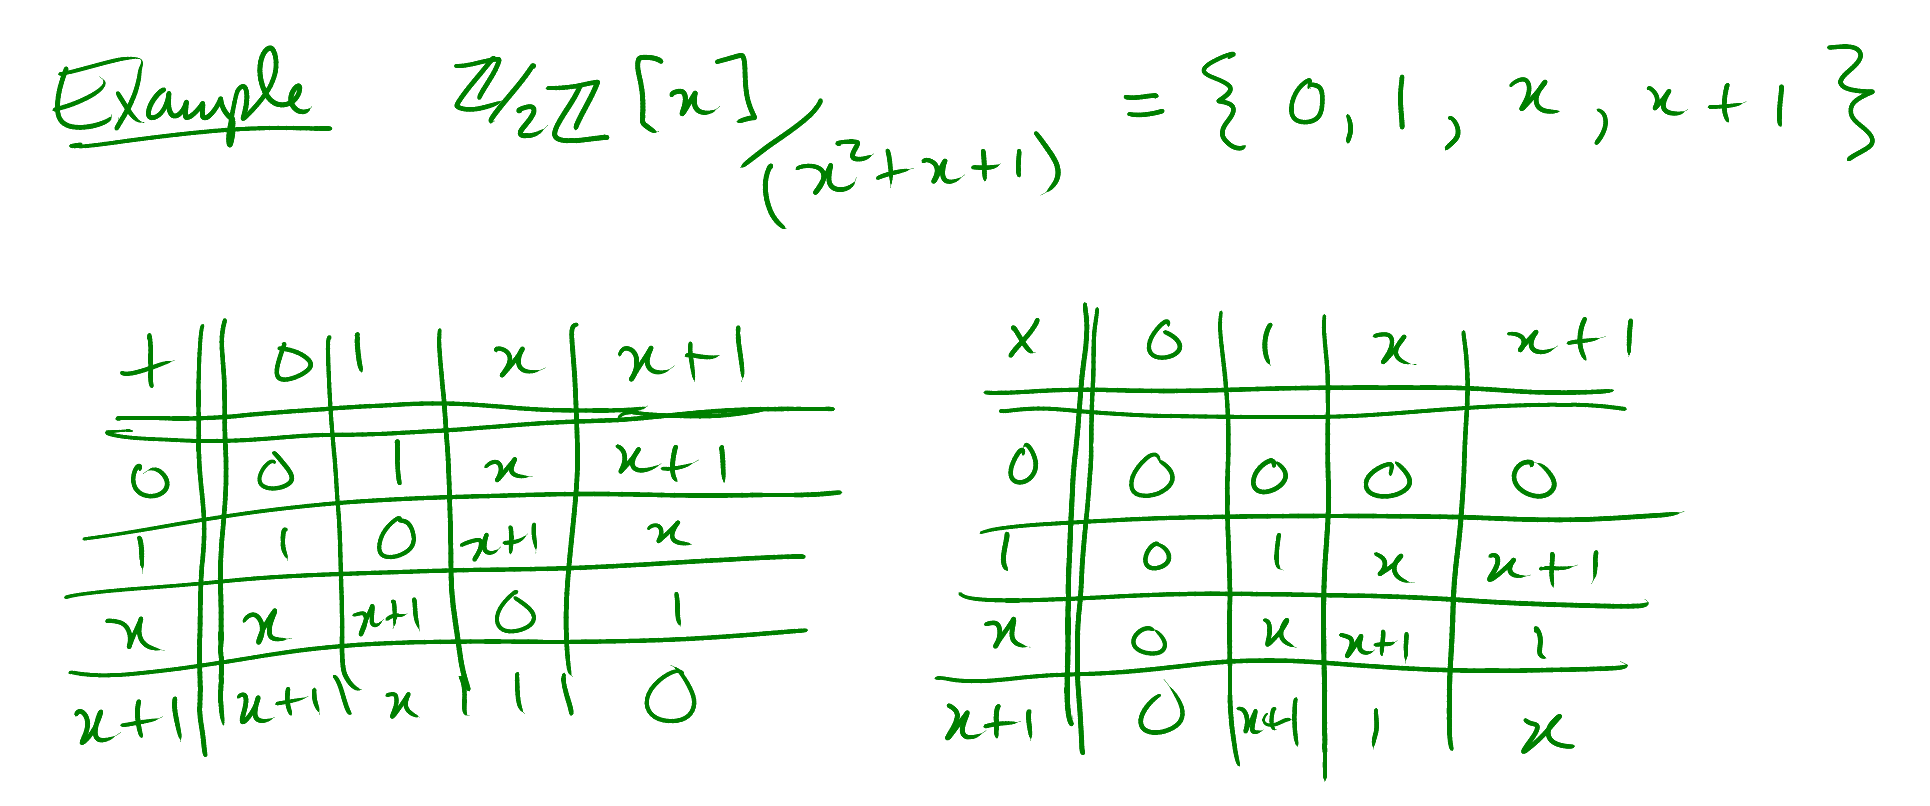
\includegraphics[width=0.9\textwidth]{f1.png}

\section{Elliptic Curves}

\begin{figure}
	\begin{center}
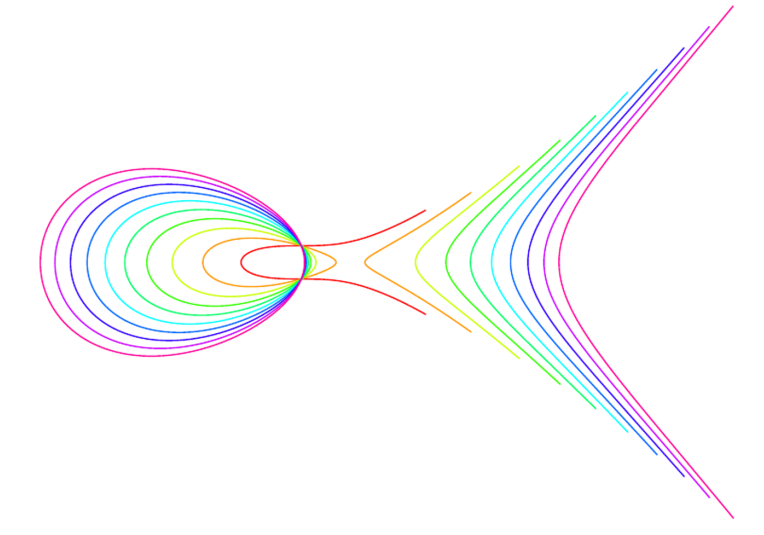
\includegraphics[width=0.7\textwidth]{curve-rainbow.png}
	\end{center}
	\caption{A variety of elliptic curves.  The rainbow colours vary with the coefficients $a,b,c$ of the Weiestrass equation $y^2 = x^3 + ax^2 + bx + c$}
\label{fig:ellcurve-rainbow}
\end{figure}

\begin{figure}
	\begin{center}
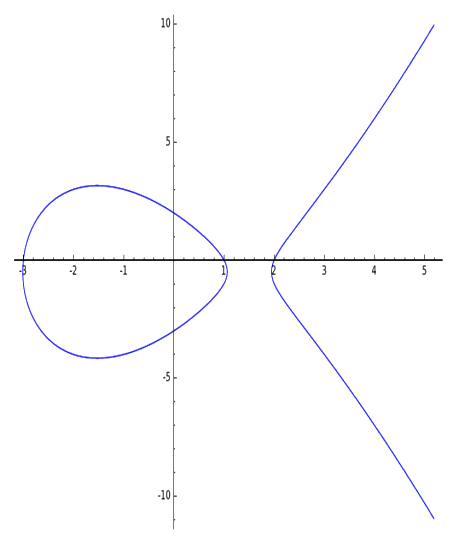
\includegraphics[width=0.4\textwidth]{curve-eg.png}
	\end{center}
	\caption{An example of an elliptic curve graphed over the real numbers}
\label{fig:ellcurve-eg}
\end{figure}

\subsection{What is an elliptic curve?}

\KS{add an example computing all pts mod p}

% >>> AI-GENERATED EXAMPLE (needs review) >>>
\begin{example}
Let us find \emph{all} points of the elliptic curve $E: y^2 \equiv x^3 + 2x + 4 \pmod{5}$.  (This is the curve we will use for the group-law example below.)  A point is a pair $(x,y)$ with $x, y \in \ZZ/5\ZZ$ satisfying the equation, together with the special point at infinity $\infty$.

We proceed by trying each value of $x \in \{0,1,2,3,4\}$, computing the right-hand side $x^3 + 2x + 4 \pmod 5$, and asking whether it is a square modulo $5$.  The squares modulo $5$ are
\[
0^2 \equiv 0, \quad 1^2 \equiv 1, \quad 2^2 \equiv 4, \quad 3^2 \equiv 4, \quad 4^2 \equiv 1 \pmod 5,
\]
so the nonzero squares are $\{1, 4\}$; a value of $1$ has square roots $\pm 1 = \{1, 4\}$, and a value of $4$ has square roots $\pm 2 = \{2, 3\}$.

\begin{center}
\begin{tabular}{c|c|c}
$x$ & $x^3 + 2x + 4 \pmod 5$ & $y$ with $y^2 \equiv$ this \\
\hline
$0$ & $4$ & $2, 3$ \\
$1$ & $7 \equiv 2$ & none \\
$2$ & $16 \equiv 1$ & $1, 4$ \\
$3$ & $37 \equiv 2$ & none \\
$4$ & $76 \equiv 1$ & $1, 4$ \\
\end{tabular}
\end{center}

Collecting the solutions, the curve $E$ has exactly seven points:
\[
(0,2), \quad (0,3), \quad (2,1), \quad (2,4), \quad (4,1), \quad (4,4), \quad \text{and} \quad \infty.
\]
In particular, the points $P = (0,2)$ and $Q = (2,4)$ used in the next example do lie on $E$.
\end{example}
% <<< END AI-GENERATED EXAMPLE <<<

For our purposes, an elliptic curve is an equation of the form $y^2 = x^3 + ax^2 + bx + c$ (this is called \textbf{Weierstrass form}).  Given an equation like this, we might be interested in the solutions, or \textbf{points} of the elliptic curve, over a particular field.  Over $\RR$, the points can be drawn with a graph, as in Figure~\ref{fig:ellcurve-eg}.

One thing to notice about the graph is that there's a reflectional symmetry across the $x$-axis, thanks to the particular form the of the equation.  That is, if $(x,y)$ is a point, then so is $(x,-y)$.  This will be useful later.

The other thing to notice about the curve is that when we intersect it with a line, we get three points, at least generically.  To see this, imagine combining a line $y = mx + n$ with the curve equation given above.  We would begin by substituting:
\[
(mx+n)^2 = x^3 + ax^2 + bx + c,
\]
and this result is a cubic equation in $x$, which can have three solutions.  Over the complex numbers, it will always have three solutions, but over the real numbers, you might not see them all.  See Figure~\ref{fig:ellcurve-options}.

\begin{figure}
	\begin{center}
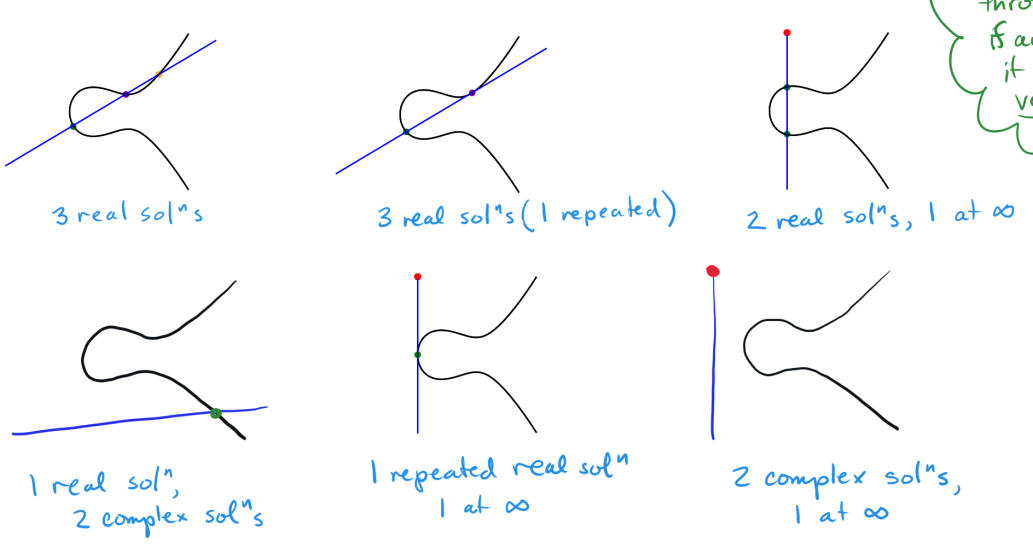
\includegraphics[width=0.8\textwidth]{curve-3pts.png}
	\end{center}
	\caption{Examples of the intersection of a line with an elliptic curve.}
\label{fig:ellcurve-options}
\end{figure}

However, there is a useful fact.

\begin{fact}\label{fact:3pts}
    If two points on the elliptic curve have coordinates in a field $F$ (for example, $F = \RR$ or $F = \CC$ or $F = \QQ$) lie on a non-vertical line $L$, then the line $L$ passes through exactly three points (the original two and one more), all with coordinates in $F$.
\end{fact}

This fact allows us to create an \textbf{addition law} on the elliptic curve.  
It turns out that the way to accomplish this is to set the following simple rules:

\begin{enumerate}
    \item There's a magical point of the elliptic curve called the \textbf{point at infinity}, denoted $\infty$, that lies on every vertical line.
    \item If three points $P$, $Q$, $R$ of the elliptic curve are on a shared line, then $P+Q+R = \infty$.
\end{enumerate}

If we follow these rules to their logical conclusion, then we get a nice addition law on the curve, where $\infty$ is the identity element.  

The first thing we discover, as a consequence of our rules, is that:

\begin{fact}
    The points on any vertical line are $\infty$, $R$ and $-R$.
\end{fact}

This "fixes" Fact~\ref{fact:3pts} so that it's true for vertical lines also.  It also means that if we have $R$ and we want $-R$, we just need to draw a vertical line through $R$ and take the other intersection point.  By the symmetry we observed earlier, $R = (x,y)$, then $-R = (x,-y)$.

Now, suppose $P$, $Q$ and $R$ are points of the curve lying on a line.  Then, by our rules, $P+Q+R= \infty$, which means $R = -(P+Q)$.  Using the vertical line trick, we can get $P+Q$ from $R$.

This gives us the addition law for adding two points $P$ and $Q$ on the elliptic curve $E$.

\begin{enumerate}
    \item Take the line $L$ through $P$ and $Q$.
    \item Let $R$ be the third intersection point of $L$ with $E$.
    \item Take the vertical line $V$ through $R$.
    \item Let $P+Q$ be the other intersection point of the vertical line with $E$ (not $\infty$).
\end{enumerate}

This calculation is illustrated in Figure~\ref{fig:ellcurve-law}.  However, for cryptographic purposes, we plan to do it in the ring (actually a finite field) $\ZZ/p\ZZ$.  So we will do it purely by algebra; all the notions (like line, etc.) are algebraic notions, captured by algebraic manipulations.  This is best illustrated by an example.


\begin{figure}
	\begin{center}
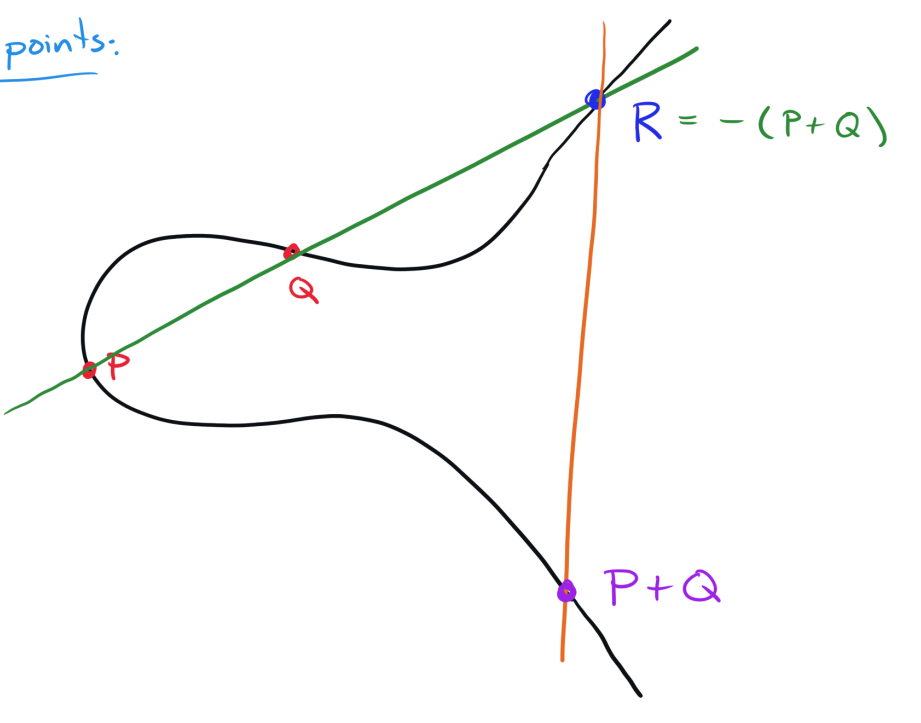
\includegraphics[width=0.4\textwidth]{curve-add.png}
	\end{center}
	\caption{An illustration of the group law on an elliptic curve.}
\label{fig:ellcurve-law}
\end{figure}

\begin{example}
We will work in $\ZZ/5\ZZ$.
    Let $y^2 \equiv x^3 + 2x + 4 \pmod{5}$ be an elliptic curve, called $E$.  Our task is to add the two points $P = (0,2)$ and $Q = (2,4)$.  
    
    First, we can verify (just to reassure ourselves) that these points are on the curve, by plugging them into the equation.  For example, for $P$,
    \[
    y^2 \equiv 2^2 \equiv 4 \pmod{5}, \quad
    \text{ and } \quad
    x^3 + 2x + 4 \equiv 0^3 + 2 \cdot 0 + 4 \equiv 4 \pmod{5}.
    \]
    Since we obtained the same answer from both calculations, we see that $P$ is indeed on the curve $E$.  
    
    \begin{checkin}
        Verify that $Q$ is on the curve.
    \end{checkin}
    \begin{aisolution}
    For $Q = (2,4)$ we compute both sides modulo $5$: the left side is $y^2 \equiv 4^2 \equiv 16 \equiv 1 \pmod 5$, and the right side is $x^3 + 2x + 4 \equiv 2^3 + 2\cdot 2 + 4 \equiv 8 + 4 + 4 \equiv 16 \equiv 1 \pmod 5$.  They agree, so $Q$ lies on $E$.
    \end{aisolution}

    To begin the group law calculation, we find the line $L$ through $P$ and $Q$.  This involves finding the slope, which is rise over run:
    \[
    \text{slope} \equiv  \frac{4-2}{2-0} \equiv \frac{2}{2} \equiv 1 \pmod{5}.
    \]
    Since $P$ is on the line $y \equiv x + n$, we have $2 \equiv 1 \cdot 0 + n$ so the $y$-intercept $n$ is $2$ and $L$ is the line
% AI-FLAGGED ORIGINAL:
%    Since $P$ is on the line $y \equiv 2x + n$, we have $2 \equiv 2 \cdot 0 + n$ so the $y$-intercept $n$ is $2$ and $L$ is the line
%    \[
%    L : y \equiv 2x + 2 \pmod{5}.
%    \]
    \[
    L : y \equiv x + 2 \pmod{5}.
    \]
\KS{Fixed by AI: the slope was just computed as $1$ (not $2$), so the line through $P,Q$ is $y\equiv x+2$. Check: $Q=(2,4)$ satisfies $2+2=4$, whereas $2\cdot2+2=6\equiv1\neq4$. (The substitution below already uses $(x+2)^2$, i.e.\ slope $1$.)}

    Next, we find the third intersection point of $L$ and $E$.  To do this, we substitute $L$ into $E$:
    \[
% AI-FLAGGED ORIGINAL:
%    (x+2)^2 \equiv x^3  + 3 x + 4 \pmod{5}.
    (x+2)^2 \equiv x^3  + 2 x + 4 \pmod{5}.
    \]
\KS{Fixed by AI: the right-hand side is the curve $x^3+2x+4$, not $x^3+3x+4$. Indeed $(x+2)^2=x^2+4x+4$ and $x^3+2x+4-(x^2+4x+4)=x^3-x^2-2x$, matching the simplified cubic below.}
    Simplifying,
    \[
    x^3 - x^2 -2x \equiv 0 \pmod{5}.
    \]
    The roots of this equation are $0,2,4$.  One quick slick way to do this is to use the fact that the second coefficient of a cubic is -1 times the sum of the roots, i.e. if we write $R = (x_R,y_R)$, then 
    \[
    0 + 2 + x_R \equiv -(-1) \equiv 1 \pmod{5}.
    \]
    So $x_R = 4$ and we can plug into $L$ to obtain $y_R \equiv x_R + 2 \equiv 4 + 2 \equiv 1 \pmod{5}$.\KS{Fixed by AI: the line is $y\equiv x+2$ (slope $1$), so $y_R\equiv x_R+2\equiv4+2\equiv1$. The original ``$2x_R+2\equiv2\cdot4+2$'' used the wrong slope, and moreover $2\cdot4+2=10\equiv0\neq1$.}  So the third intersection point is $R = (4,1)$.

    Finally, the last step is to reflect $R$ across the $x$-axis, which means changing the sign on the $y$ coordinate (keep in mind $-1 \equiv 4 \pmod{5}$):
    \[
    P + Q = -R = (4,4).
    \]
    We are done!
\end{example}

Let's record that nice \textbf{trace trick}:

\begin{fact}
    Given a cubic $x^3 + ax^2 + bx + c$, the three roots add up to $-a$.
\end{fact}

\begin{checkin}
    Can you prove the trace trick?\footnote{Hint: Try expanding $(x+r)(x+s)(x+t)$.}
\end{checkin}
\begin{aisolution}
If the cubic $x^3 + ax^2 + bx + c$ has roots $r,s,t$, then it factors as $(x-r)(x-s)(x-t)$.  Expanding,
\[
(x-r)(x-s)(x-t) = x^3 - (r+s+t)x^2 + (rs+rt+st)x - rst.
\]
Matching the coefficient of $x^2$ gives $a = -(r+s+t)$, i.e. $r+s+t = -a$.
\end{aisolution}

Also, notice that we have to be careful to keep in mind we are working modulo $p$.  This means we can't divide by any multiple of $p$, when taking the slope, for example.

\subsection{Double points}

There's still the issue of lines that pass through a point twice.  This is the same as being tangent at that point.  \KS{more here}



\subsection{Projective space}

The definition of projective space:

\[
\mathbf{P}^n_{\FF_q} := \{ \mathbf{v} \in \FF_q^{n+1} : \mathbf{v} \neq \mathbf{0} \} / \sim
\]
where $\sim$ indicates that we identify as being the same any two vectors which share the same direction.  In other words,
\[
\mathbf{v} \sim \mathbf{w}
\]
means exactly that
\[
\mathbf{v} = \lambda \mathbf{w}
\]
for some non-zero scalar $\lambda$.  That is, we organize the vectors of $\FF_q^{n+1}$ (besides the zero vector) into groupings according to direction.  

Here's an example.  In $\PP^1_{\FF_5}$, we have the following elements (each element is a grouping, or \textbf{equivalence class} of vectors we are thinking of as being `the same' or `equivalent'):
\begin{align*}
&\{ [0,1], [0,2], [0,3], [0,4] \} \\
&\{ [1,0], [2,0], [3,0], [4,0] \} \\
&\{ [1,1], [2,2], [3,3], [4,4] \} \\
&\{ [1,2], [2,4], [3,1], [4,3] \} \\
&\{ [1,3], [2,1], [3,4], [4,2] \} \\
&\{ [1,4], [2,3], [3,2], [4,1] \} 
\end{align*}
In other words, these are the six elements of $\PP^1_{\FF_5}$.  I write the vectors with square brackets to remind you we are using this equivalence relation and working in projective space, so when I write $[0,1]$ it is short form for the whole equivalent class listed in the first line above.  I can use any element of the equivalence class to denote the entire equivalence class.  In other words, it is perfectly meaningful and true to write
\[
[0,1] = [0,2]
\]
etc.

\begin{quiz}
    Verify that every non-zero vector of $\FF_5^2$ occurs somewhere in the lists above.  What is the principle of organization that I used to list them all here?  Choose two random elements from the same line, and figure out what is the corresponding $\lambda$ in the explanation of $\sim$ given above.
\end{quiz}
\begin{aisolution}
There are $5^2 - 1 = 24$ non-zero vectors in $\FF_5^2$, and the six lists contain $6 \times 4 = 24$ vectors---exactly accounting for all of them (each appears once).  The principle of organization is grouping by \emph{direction}: two vectors are in the same list exactly when one is a non-zero scalar multiple of the other.  Each class is named by a normalized representative---either $[0,1]$, or $[1,m]$ with the first coordinate scaled to $1$.  For instance, take $[1,2]$ and $[2,4]$ from the same line: here $[2,4] = 2\cdot[1,2]$, so $\lambda = 2$.
\end{aisolution}

To count the elements in the projective space $\PP^n_{\FF_q}$, we first count the number of elements in the underlying vector space:
\[
\# \FF_q^{n+1} = q^{n+1}.
\]
However, we are throwing out the zero vector, so we have
\[
q^{n+1}-1
\]
vectors.  Next, we are identifying the vectors into groups.  For each non-zero vector, there are $q-1$ non-zero scalars we could multiply it by to get a vector that is the same in direction (but possibly different in length).  So each equivalence class of vectors is of size $q-1$.  So the total size of projective space is
\[
\# \PP^n_{\FF_q} = \frac{q^{n+1}-1}{q-1}.
\]

\begin{quiz}
    Verify the formula above for the example above.  Don't just verify the conclusion, but verify each step of the explanation in the case of the example above (number of non-zero vectors, size of each equivalence class).
\end{quiz}
\begin{aisolution}
Here $q = 5$ and $n = 1$.  The underlying vector space $\FF_5^2$ has $q^{n+1} = 5^2 = 25$ vectors; removing the zero vector leaves $25 - 1 = 24$ non-zero vectors.  Each equivalence class has size $q - 1 = 4$ (the four non-zero scalar multiples), which matches the four vectors listed on each line above.  Hence the number of classes is $24/4 = 6$, agreeing with the formula
\[
\#\PP^1_{\FF_5} = \frac{q^{n+1}-1}{q-1} = \frac{25-1}{5-1} = \frac{24}{4} = 6.
\]
\end{aisolution}



\subsection{Factoring with elliptic curves}

\subsubsection{An example motivating the key idea}

Consider the three closely related examples below.  As the author of this textbook, I strongly encourage you, the reader, to attempt each question in turn before you read the solution.  As they say, math is not a spectator sport.  And anyway, you don't want to miss this one, it involves blowing up the universe.\\

\textbf{Question 1.}  Consider the curve $y^2 \equiv x^3 +2x + 1$ modulo 5.  Compute the addition of the two points $P = (3,3)$ and $Q = (1,2)$ by hand.  \\

\textbf{Soln.} The first step is to compute the slope, $-1/-2 \equiv 1/2 \equiv 3 \pmod{5}$.  The line that joins these points is $y \equiv 3x - 1$.  The intersection with the curve is $(3x-1)^2 \equiv x^3 + 2x + 1$, which becomes $x^3 + x^2 + 3x \equiv 0$.  By the trace trick, we know $-1 \equiv 3 + 1 + x_R$, so we obtain $x_R \equiv 0$, which gives $y \equiv -1$.  Reflecting across the axis, the result is $P+Q = (0,1)$.\\

\textbf{Question 2.}
On the curve $y^2 \equiv x^3 +2x + 1$ modulo 7, try to compute the addition of the two points $P = (0,6)$ and $Q = (0,1)$ by hand.\\

\textbf{Soln.} We begin by considering the slope, rise over run:  $-5/0$.  This is a division by zero!  Boom, the universe explodes!  In fact, looking closer at the problem, we observe that $P = -Q$, so that $P+Q = \infty$.  The slope `exploding' to infinity alerts us to this fact, if we have failed to observe it, because the division by $0$ indicates the line between $P$ and $Q$ is vertical.\\

\textbf{Question 3.}  On the curve $y^2 \equiv x^3 +2x + 1$ modulo 35, try to compute the addition of the two points $P = (28,13)$ and $Q = (21,22)$ by hand.\\

\textbf{Soln.} We begin by considering the slope, rise over run:  $-9/7$.\KS{Fixed by AI: the run is $x_P-x_Q=28-21=7$ (positive), so the slope is $-9/7$, not $-9/-7\equiv9/7$. This matters for the ``shadow'' reasoning: $-9/7\equiv1/2\equiv3\pmod5$ matches the slope in Question~1, whereas $9/7\equiv2\pmod5$ would not.}  Since we are working modulo $35$, we must compute the inverse of $7$ modulo $35$.  But if we begin that process (which involves an extended Euclidean algorithm), we will come up against the fact that $7$ is not invertible modulo $35$, since they share a non-trivial factor of $7$.  Boom!  The universe explodes as we attempt to divide by something which is not invertible!  In calmer parlance, we cannot proceed.\\

Now let's step back and analyse the situation.  Observe the following things:
\begin{enumerate}
    \item The three problems all involve the same elliptic curve considered with respect to different moduli.
    \item Since $5$ and $7$ both divide $35$, the curve and points in Question 3 have well-defined residues modulo $5$ and $7$.  Then $P$ and $Q$ in Question $3$ reduce to the $P$ and $Q$ in Questions 1 and 2.  
        \item The third problem involves considering an elliptic curve modulo a composite number $35$.  We have never done this sort of thing before, and reflecting upon our experience above, perhaps it is a dangerous thing to do!
\end{enumerate}

Because information modulo $35$ reduces to information modulo $5$ and $7$ (this is one direction of Sunzi's Theorem), any arithmetic we do in Question 3 has `shadow arithmetic' happening modulo $5$ and $7$.  Because the curve and points in Question 3 reduce to those provided in Questions 1 and 2, the `shadow' of Question 3's solution is the work done in Questions 1 and 2.  In particular, since Question 2 fails on division by $0 \pmod{7}$, Question 3 fails on division by a multiple of $7$.

What lesson do we take from this?  The pessimist will  throw out the idea of curves modulo composite numbers as flawed and useless.  The creative optimist will reinterpret the `failure' (Boom!  No more universe!) encountered in Question 3 as a success:  it actually results in the factorization of $35$!  That is, when we try to invert $7$, we take $\gcd(7,35) = 7$, discovering a factor.

Mathematicians are optimists.

This idea can be turned into a factoring algorithm for a composite number $N$.  The fundamental approach is to do a bunch of arithmetic on an elliptic curve modulo $N$, and hope that one of the computations `blows up' by a failure to invert when computing the slope.  If this happens, we have found some residue $r$ not coprime to $N$, so we take $\gcd(r,N)$ to get a factor of $N$.

The only remaining piece of the puzzle is to find a clever way to encourage the `explosion' to happen.  Instead of doing random computations on the elliptic curve, we should be clever about designing `dangerous' ones that might explode.

Let your inner destructive force emerge!

\subsubsection{Pollard's $p-1$ factoring algorithm}

Let $n = pq$ be an RSA modulus.  There is a factoring method of Pollard that works especially well when $p-1$ factors as a product of small primes, but $q-1$ does not.  It does not have to do with elliptic curves, but the elliptic curve method is based upon (in analogy to) this method.

This is based on a common paradigm:  work modulo $n$, and you are working modulo $p$ and $q$ by the Chinese Remainder Theorem, although you cannot `see' this without knowing $p$ and $q$.  In this case, the algorithm is to compute a long sequence of powers of a residue $a$ modulo $m$:
\begin{equation}
    \label{eqn:p-1seq}
a \rightarrow a^2 
\rightarrow a^{3!}
\rightarrow a^{4!}
\rightarrow a^{5!}
\rightarrow a^{6!}
\rightarrow a^{7!}
\rightarrow \cdots
\end{equation}
\KS{Fixed by AI: the fifth term was written $a^{5!!}$ (double factorial); it should be $a^{5!}$ to match the factorial sequence (cf.\ the CRT version below, which has $a_1^{5!}$).}
To compute this, we can first square, then cube, then raise to the fourth power, etc.

Behind the scenes, so to speak, the Chinese remainder theorem tells us that our arithmetic efforts are simultaneously reproduced modulo $p$ and modulo $q$.  Under the isomorphism of CRT,
\[
(\ZZ/n\ZZ)^* \cong (\ZZ/pZZ)^* \times (\ZZ/q\ZZ)^*, \quad a \mapsto (a_1,a_2).
\]
Note that in the map above, $a_1$ is just the residue of $a$ modulo $p$ and $a_2$ is just the residue of $a$ modulo $q$.
Thus, there is an inaccessible isomorphic version of the sequence \eqref{eqn:p-1seq} above:
\[
(a_1,a_2) \rightarrow (a_1^2, a_2^2)
\rightarrow (a_1^{3!}, a_2^{3!})
\rightarrow (a_1^{4!}, a_2^{4!})
\rightarrow (a_1^{5!}, a_2^{5!})
\rightarrow (a_1^{6!}, a_2^{6!})
\rightarrow (a_1^{7!}, a_2^{7!}) \ldots
\]
We can't see this sequence directly (because we don't know $p$ and $q$), but we know it is there (by CRT).  What we can do is 
build a `detector' for when $(a_1^{B!},a_2^{B!})$ becomes $(1,*)$ or $(*,1)$ (the $*$ represents any value other than $1$).  For example, when
\[
(a_1^{B!}, a_2^{B!}) \equiv (1, x)
\]
where $x \not\equiv 1 \pmod q$, then we have
\[
a_1^{B!} \equiv 1 \pmod{p}, \quad a_2^{B!} \not\equiv 1 \pmod{q}
\]
that is, $p$ divides $a^{B!}-1$ but $q$ does not.  Therefore,
\[
\gcd(a^{B!}-1, n) = p.
\]

\textbf{The algorithm:}  
The algorithm, therefore, is to compute the sequence $a^{B!}$ (that is, \eqref{eqn:p-1seq}) by successive modular exponentiation, and at each step, compute $\gcd(a^{B!}-1,n)$.  We hope to get a proper factor of $n$.  If we get the gcd to be $n$, we know we have gone `too far' (both values $a_1^{B!}$ and $a_2^{B!}$ have reached 1, and they will not change if we keep going) and should stop, having failed.

\begin{example}
    Let's factor $n = 5893$.  We choose $a \equiv 2 \pmod{n}$.  Then we compute a chain of factorials:
    \[
    a\equiv 2 \rightarrow
    a^{2!} \equiv 4 \rightarrow
     a^{3!} \equiv 64 \rightarrow
      a^{4!} \equiv 5738 \rightarrow
       a^{5!} \equiv 3019 \rightarrow
        a^{6!} \equiv 119 \rightarrow
        a^{7!} \equiv 2770 \rightarrow
    \]
    Taking the $\gcd$ of $a^{k!} -1$ with $n$ at each stage, we get
    \begin{align*}
    \gcd(a-1,n) &= \gcd(1,n) = 1 \\
    \gcd(a^{2!}-1,n) &= \gcd(3,n) = 1 \\
    \gcd(a^{3!}-1,n) &= \gcd(63,n) = 1 \\
    \gcd(a^{4!}-1,n) &= \gcd(5737,n) = 1 \\
    \gcd(a^{5!}-1,n) &= \gcd(3018,n) = 1 \\
    \gcd(a^{6!}-1,n) &= \gcd(118,n) = 1 \\
    \gcd(a^{7!}-1,n) &= \gcd(2769, n) = 71 \\
    \end{align*}
    Our gcd `detector' has alarmed at $7!$, alerting us to a factor of $71$, so we can stop the chain at that point.  The full factorization of $n$ is $5893 = 71 \cdot 83$.  Notice that $p-1 = 71-1 = 70 = 2 \cdot 5 \cdot 7$ but $q-1 = 83 - 1 = 82 = 2 \cdot 41$, so the `smooth' $p-1$ showed up in the detector first (as soon as all its primes were in the factorial exponent).
\end{example}



\textbf{When this works and a lesson for RSA:}
This algorithm is not a general factoring algorithm, because it will only work when $p-1$ is made up of small factors, so it is likely to divide the highly composite number $B!$.  Therefore, we have a lesson for RSA:  avoid primes with this property.  Instead, choose what are called \emph{safe primes}, those primes $p$ for which $p-1$ is two times a prime (observe that we can't help it being even, but otherwise we can make it factor very little).  To find such safe primes, it is most expedient to try primes $p_0$ of size around $\sqrt{n}/2$, and then check whether $p = 2p_0+1$ is prime.  If it is, it's a safe prime.


\subsubsection{Elliptic Curve Factoring}

This is very similar in spirit to Pollard $p-1$ factoring.  Instead of working with powers of $a$ in $(\ZZ/n\ZZ)^*$, we work with multiples of a point $P$ on an elliptic curve $E$ modulo $n$.  I will try to emphasize the similarities.

Choose an elliptic curve $E$ and point $P$ on $E$ modulo $n$.  An expedient way to do this is to pick $P$ first, and then solve for the constant term of $E$ to make it a valid point on $E$.

We work on $E$ modulo $n$, but by CRT, since all our elliptic curve computations are modular arithmetic computations, this is `secretly' working on $E$ modulo $p$ and modulo $q$.  That is, a point $P =(x,y)$ on $E$ modulo $n$ maps to two points:
\[
P_1 = (x \pmod{p}, y \pmod{p}) \text{ on } E_1 \pmod{p}, \text{, and }
P_2 = (x \pmod{q}, y \pmod{q}) \text{ on } E_2 \pmod{q}, 
\]
The curve $E_1$ and $E_2$ have the same equation as for $E$, just considered modulo $p$ and $q$ respectively.

So, we compute a sequence of points on $E$ modulo $n$:
\begin{equation}
    \label{eqn:ecfactor}
P \rightarrow 2!P
\rightarrow 3!P
\rightarrow 4!P
\rightarrow 5!P
\rightarrow 6!P
\rightarrow 7!P
\rightarrow \cdots
\end{equation}
while CRT guarantees an inaccessible sequence
\[
(P_1,P_2) \rightarrow (2!P_1,2!P_2)
\rightarrow (3!P_1, 3!P_2)
\rightarrow (4!P_1, 4!P_2)
\rightarrow (5!P_1, 5!P_2)
\rightarrow (6!P_1, 6!P_2)
\rightarrow (7!P_1, 7!P_2)
\rightarrow \cdots
\]
We can't see this sequence directly (because we don't know $p$ and $q$), but we know it is there (by CRT).  What we can do is build a `detector' for when $(B!P_1, B!P_2)$ becomes $(\infty, *)$ or $(*, \infty)$ where $*$ represents any point on the elliptic curve which is not the point at infinity.

How the detector works is slightly different than in the $p-1$ case.  When
\[
(B!P_1, B!P_2) \equiv (\infty ,X)
\]
where $X$ is not the point at $\infty$, then we have that
\[
B!P_1 = [0,1,0]
\]
as a projective point.  This means that when we compute the point, we obtain
\[
B!P_1 = (a/d,b/d) = [a,b,d].
\]
where $d \equiv 0 \pmod p$.  Thus, in the algorithm for adding points, we end up dividing by an element which is not invertible modulo $p$.  Then
\[
gcd(d,n) = p.
\]
Thus, we simply try to compute $B!P$ and watch for a non-invertible element $d$; it will contain a common factor with $n$.

\textbf{The algorithm:}  Compute the sequence \eqref{eqn:ecfactor}, until the algorithm fails because you try to invert something modulo $d$ which is not invertible.  (If doing this by hand, you'd be doing the extended euclidean algorithm to get an inverse modulo $n$ and get a gcd which is not $1$.)  Then that element will have a common factor with $n$, so compute $\gcd(d,n)$.  If you get $\gcd(d,n) = n$, you have failed and should re-start with another elliptic curve and point.

\begin{example}
    Let's factor $n=18923$.  To find a random curve and point, it's actually easier to choose the point first!  Suppose we pick $P = (0,1)$.  Then we can look for a curve that has that point.  For example, we could start with $y^2 = x^3 + x + \cdots$ and fill in the constant term so that when we plug in $(0,1)$, it works.  That means we choose $y^2 = x^3 + x + 1$.  Now we compute the factorial multiples of $P$:
    \begin{align*}
     P &= (0,1) \\
     2!P &= (4731, 7095) \\
     3!P &= (14478, 16509) \\
     4!P &= (17852, 18391) \\
     5!P &= (7112, 8383) \\
     6!P &= (11684, 10413)
    \end{align*}
    So far so good.  But then when we try to multiply this point by $7$ to obtain $7!P$, Sage reports an error -- 17272 is not invertible.  So it must have a common factor with $n$.  We check:
    \[
    \gcd(17272,18923) = 127. 
    \]
    In fact, $n = 127 \cdot 149$.
\end{example}


\textbf{When it works.}  This will work when the order of $P$ on $E_1$ divides $B!$ but on $E_2$ it does not.  We know the order of $P$ will divide the order of the group, i.e. the number of points on the curve modulo $p$.  Since the number of points on an elliptic curve, and therefore the order of the point $P$, varies, you can try again when you fail.  This makes it a general factoring method.  It works best, however, when $n$ has a small factor, since a smaller $p$ means a smaller curve mod $p$.

In fact, it is subexponential!  It was the state of the art before quadratic sieve was improved to number field sieve.  It is still used to find small factors before calling on the number field sieve.



\subsection{Elliptic Curve Discrete Logarithm Problem}

Let $E$ be an elliptic curve.
The Elliptic Curve Discrete Logarithm Problem is to find $n$ when we are given the points $P$ and $Q = nP$ on the elliptic curve $E$.

This problem is analogous to the discrete logarithm problem modulo $p$ and the discrete logarithm problem in finite fields.

The Baby-Step-Giant-Step and Collision/Birthday attacks work in all cases, since they only use the group structure.  In the language of the elliptic curve discrete logarithm problem, we have a point $P$ of some order, say $r$.  We take $N = \lceil \sqrt{r} \rceil$ and make two lists:

Baby steps:
\[
P, 2P, 3P, 4P, \ldots
\]
Giant steps:
\[
Q, Q - NP, Q-2NP, Q-3NP, \ldots
\]

We hope for a collision, which would give a relationship
\[
jP = Q - kNP
\]
which we can then solve as
\[
Q = (j + kN)P.
\]

Compare this formalism to Section~\ref{sec:baby-giant} (2.8.1).\KS{AI: \texttt{\textbackslash ref\{sec:baby-giant\}} here is undefined (renders as "LABEL:sec:baby-giant") -- the label is missing at the Baby-Step Giant-Step subsubsection; add it there. Also, the hand-written "(2.8.1)" should then become the automatic reference number.}

\subsection{Elliptic Curve Diffie-Hellman}

\subsection{Elliptic Curve El Gamal}

Elliptic Curve El Gamal is exactly like regular El Gamal except that we substitute the collection of points on $E$ modulo $p$, denoted $E(\FF_p)$, for the multiplicative group $(\ZZ/p\ZZ)^*$.  This means that we are working on a cycle of points\footnote{Created by ChatGPT, which is good at tikz!}

\begin{center}
\begin{tikzpicture}[->, >=Latex, shorten >=2pt, thick]
    \def\R{2.2cm}
    % dots on the ring (clockwise from the top)
    \node[circle, fill=black, inner sep=1.7pt] (1) at (90:\R) {};
    \node[circle, fill=black, inner sep=1.7pt] (2) at (18:\R) {};
    \node[circle, fill=black, inner sep=1.7pt] (3) at (-54:\R) {};
    \node[circle, fill=black, inner sep=1.7pt] (4) at (-126:\R) {};
    \node[circle, fill=black, inner sep=1.7pt] (5) at (-198:\R) {};
    % labels, pushed outside the ring so the arcs never cross them
    \node at (90:{\R+0.5cm})  {$P$};
    \node at (18:{\R+0.6cm})  {$2P$};
    \node at (-54:{\R+0.6cm}) {$3P$};
    \node at (-126:{\R+0.5cm}) {$\cdots$};
    \node at (-198:{\R+1.0cm}) {$NP=\infty$};
    % arrows around the cycle
    \path (1) edge[bend right=12] (2)
          (2) edge[bend right=12] (3)
          (3) edge[bend right=12] (4)
          (4) edge[bend right=12] (5)
          (5) edge[bend right=12] (1);
\end{tikzpicture}
\end{center}

instead of the cycle of powers of $g \in (\ZZ/p\ZZ)^*$.  The cycle is of size $N$, where $N$ is the order of $P$.  The \textbf{order} of a point $P$ on an elliptic curve is the smallest positive integer $N$ so that $NP = \infty$.

In what follows, it might help to observe that lowercase $a,b,k$ are integers and uppercase $P, M, B, K, C$ are points on the curve.

     {\bf Setup:}  $E$ an elliptic curve defined modulo $p$, $P$ a point on $E$ of order $N$.
     \vspace{1em}

     \begin{tabular}{ccc}
       Alice & & Bob \\
       \hline
       Message: $M \in E(\FF_p)$ & &  Secret key: $0 < b < N$ \\
       $B$ & $\longleftarrow$ & Public key: $B = bP$ \\
       Ephemeral secret key: $0 < k < N$ & &  \\
       Ephemeral public key: $K = kP$ & &  \\
       Masked message: $C = M + kB$ & &  \\
       Ciphertext: $(K,C) = (kP, M + kB)$ & $\longrightarrow$ & $(K,C)$ \\
					      & & Decryption: $C - bK$ \\
      \end{tabular}
      \vspace{3em}
      

      Correctness of the decryption is guaranteed by the following computation:
      \[
      C - bK = C - bkP = C - kB = M
      \]


\subsubsection{Placing a message on a curve}

In order to use the EC El Gamal protocol above, we need a way to put a point onto an elliptic curve.  We discuss a fairly simple way to do this here, although in practice \KS{add more}.

Suppose our message $m$ is already turned into an integer.  We can block it into small parts to encrypt separately if it is too long.  We can take our message, append a small bit of padding (a predetermined number of bits, say), and then try to use it as an $x$-coordinate for a point on the curve.  To see if it is the $x$-coordinate of a valid point on the curve $y^2 = f(x)$, we need to plug it into $f(x)$ and see if the result is a square.  If so, then let $y = \sqrt{f(x)}$ (either of the two roots is fine), and we use $M = (x,y)$ as the "message" in the algorithm above.  If not, we can alter the padding and try again.

Recall that any non-zero residue modulo $p$ has a one-half probability of being a square.  So we will quickly succeed by trying a few different paddings.

This method requires that we have a method of finding square roots modulo $p$.

\subsubsection{Square roots modulo $p$}



There is a particularly simple algorithm for finding square roots modulo $p$ when $p \equiv 3 \pmod{4}$.  It is as follows:

\textbf{Algorithm to find a square root of $a$ modulo $p$.}
\begin{enumerate}
    \item Compute $k = a^{\frac{p+1}{4}} \pmod{p}$.
    \item If $k^2 \equiv a \pmod{p}$, return $k$ (this is the square root of $a$; the other is $-k$).
    \item If not, then return \textbf{failed}. (In this case there is no square root of $a$ and $k^2 \equiv -a \pmod{p}$.)
\end{enumerate}

That's it!  Notice that it is only when $p \equiv 3 \pmod{4}$ that $\frac{p+1}{4}$ is an integer.  If it is not an integer, we wouldn't be able to compute $a^{\frac{p+1}{4}}$ as a modular exponentiation.

\begin{example}
    To compute the square root of $3$ modulo $11$, we compute
    \[
    \frac{p+1}{4} = \frac{11+1}{4} = 3.
    \]
    Then we compute
    \[
    3^{\frac{p+1}{4}} \equiv 3^3 \equiv 27 \equiv 5 \pmod{11}.
    \]
    This is our candidate square root.  To check if it worked, we compute
    \[
    5^2 \equiv 25 \equiv 3 \pmod{11}.
    \]
    Since it worked, we have computed a square root of $3$, and found it to be $5$.  The full set of square roots is $\pm 5$.
\end{example}

\textbf{Why does this work?}  We return to the observation that $(\ZZ/p\ZZ)^*$ is a cyclic group.  Let $g$ be a generator.  Then taking powers of $g$, we obtain all the residues of $(\ZZ/p\ZZ)^*$, forming a single cycle. 

\begin{center}
\begin{tikzpicture}[->, >=Latex, shorten >=2pt, thick]
    \def\R{2.2cm}
    % dots on the ring (clockwise from the top)
    \node[circle, fill=black, inner sep=1.7pt] (1) at (90:\R) {};
    \node[circle, fill=black, inner sep=1.7pt] (2) at (18:\R) {};
    \node[circle, fill=black, inner sep=1.7pt] (3) at (-54:\R) {};
    \node[circle, fill=black, inner sep=1.7pt] (4) at (-126:\R) {};
    \node[circle, fill=black, inner sep=1.7pt] (5) at (-198:\R) {};
    % labels, pushed outside the ring
    \node at (90:{\R+0.5cm})  {$g$};
    \node at (18:{\R+0.6cm})  {$g^2$};
    \node at (-54:{\R+0.6cm}) {$g^3$};
    \node at (-126:{\R+0.5cm}) {$\cdots$};
    \node at (-198:{\R+1.05cm}) {$g^{p-1}=1$};
    % arrows around the cycle
    \path (1) edge[bend right=12] (2)
          (2) edge[bend right=12] (3)
          (3) edge[bend right=12] (4)
          (4) edge[bend right=12] (5)
          (5) edge[bend right=12] (1);

\end{tikzpicture}
\end{center}

Since the size of this cycle is $p-1$, which is even, the squares are exactly the powers $g^{2k}$, i.e. the even powers of $g$.  \KS{circle these on the cycle}.

So if $a$ is a square, then it is of the form $g^{2k}$ and in fact, it has order dividing $(p-1)/2$, since
\[
a^{\frac{p-1}{2}} \equiv g^{p-1} \equiv 1 \pmod{p}.
\]
So if we draw the cycle of powers of $a$ up to $(p-1)/2$, it closes in on itself, with $a^{\frac{p-1}{2}} \equiv 1$.

\begin{center}
\begin{tikzpicture}[->, >=Latex, shorten >=2pt, thick]
    \def\R{2.2cm}
    % dots on the ring (clockwise from the top)
    \node[circle, fill=black, inner sep=1.7pt] (1) at (90:\R) {};
    \node[circle, fill=black, inner sep=1.7pt] (2) at (18:\R) {};
    \node[circle, fill=black, inner sep=1.7pt] (3) at (-54:\R) {};
    \node[circle, fill=black, inner sep=1.7pt] (4) at (-126:\R) {};
    \node[circle, fill=black, inner sep=1.7pt] (5) at (-198:\R) {};
    % labels, pushed outside the ring
    \node at (90:{\R+0.9cm})  {$a = a^{\frac{p+1}{2}}$};
    \node at (18:{\R+0.6cm})  {$a^2$};
    \node at (-54:{\R+0.6cm}) {$a^3$};
    \node at (-126:{\R+0.5cm}) {$\cdots$};
    \node at (-198:{\R+0.95cm}) {$1 = a^{\frac{p-1}{2}}$};
    % arrows around the cycle
    \path (1) edge[bend right=12] (2)
          (2) edge[bend right=12] (3)
          (3) edge[bend right=12] (4)
          (4) edge[bend right=12] (5)
          (5) edge[bend right=12] (1);

\end{tikzpicture}
\end{center}

In particular, and this is the most important observation about $a$:
\[
\boxed{
a \equiv 1 \cdot a \equiv a^{\frac{p-1}{2}}a \equiv a^{\frac{p+1}{2}} \pmod{p}.
}
\]
Now, when we are in the case that $p \equiv 3 \pmod{4}$, this exponent $\frac{p+1}{2}$ is \emph{even}, so the well-defined element
\[
a^{\frac{p+1}{4}}
\]
will square to $a$:
\[
(a^{\frac{p+1}{4}})^2 \equiv
a^{\frac{p+1}{2}} \equiv a \pmod{p}.
\]





\subsection{EC\_Dual\_DRBG}

\subsubsection{Cryptographic pseudo random number generators}

True randomness is hard to come by.  But we need it for cryptography:  for example, to generate a random secret key for your private/public key pair.  Some computers use input from your keyboard taps and mouse movements to generate randomness based on the physical world around them.  But the most common source of randomness for private keys is a \textbf{pseudo-random number generator}, which is actually a deterministic algorithm whose output looks random to the eye.

For many applications, it is sufficient that the result look fairly random.  For example, such algorithms are used to generate the position of cacti in the videogame Minecraft when the world is initialized.  As long as they are fairly randomly distributed, the game is perfectly playable.

However, for a \textbf{cryptographic pseudo-random number generator}, the most important property of is that its outputs are \emph{not predictable}.  It is ok that they are in fact deterministic, if no adversary can guess the next output from known previous outputs.  The second most important property is that it can generate pseudo-random bits fairly quickly.

The algorithm has an \textbf{internal state} $s_n$ which is updated as each time step.  For example, the RANDU algorithm used on mainframes in the 1960's and 70's has an update step of the form
\[
s_{k+1} = 65539 s_k \pmod{2^{31}}.
\]
The value $s_0$ is the \textbf{seed} and this must be kept secret, because anyone who has it can run the algorithm and get all values of $s_n$.

The actual randomness that is given as output must not reveal the entire hidden state, because with that knowledge, the adversary can predict the next state and next output.  Instead, what is typically done is that a few bits of $s_k$ are revealed as the output, but most bits are kept secret.  For example, in RANDU, one might reveal the last bit of $s_{k+1}$ at each step, obtaining a stream of output bits, one per iteration.

However, RANDU is not a very good cryptographic pseudo-random number generator, because it was discovered that there was a lot of correlation between subsequent values.  The algorithm itself was just chosen for speed and looked fairly random to the eye.  But it would make a terrible cryptographic choice.

Other \textbf{linear congruential generators} have update rules
\[
s_{k+1} = a s_k + b \pmod {m}
\]
and many have better behaviour than RANDU, but none are considered suitable for cryptography.

\subsubsection{Blum Blum Shub}

An example of a cryptographic pseudo-random number generator is \textbf{Blum-Blum-Shub}.  Like the linear congruential generator, it uses modular arithmetic, which is fast for computers.  The update rule is
\[
s_{k+1} = s_k^2 \pmod{n},
\]
where $n$ is chosen to be an RSA modulus, i.e. $n=pq$ where $p$ and $q$ are large primes, and $n$ is considered hard to factor (for example, they should be \emph{safe primes} to avoid the $p-1$ factoring method etc.).  We also require $p$ and $q$ to be chosen to be $3$ modulo $4$.  The seed $s_0$ must be coprime to $n$.

At each stage, we output the smallest $\log \log n$ bits of $s_k$ as the output randomness.

The security of Blum Blum Shub comes with a guarantee of sorts:  if one can predict the next bit of a Blum Blum Shub sequence (the randomness output by the generator), with probability non-negligibly better than $1/2$ (i.e., the advantage is at worst 1/polynomial), in polynomial time, then one can solve the \textbf{quadratic residuosity problem modulo $n$} with non-negligible advantage also.

The quadratic residuosity problem is to determine, for any $a$ modulo $n$, whether $a$ is a \emph{quadratic residue}, i.e. the residue of a square modulo $n$.  For example, $3$ is a quadratic residue modulo $6$ since it is the residue of the square $9$.

Here's the original paper:
\url{https://static.aminer.org/pdf/PDF/000/120/466/comparison_of_two_pseudo_random_number_generators.pdf}

\subsubsection{EC\_Dual\_DRBG}

Another suggestion for a cryptographic pseudo random number generator was called EC\_DUAL\_DRBG by NIST.  It works as follows.  Let $E$ be an elliptic curve modulo $p$, with $k$ points, and let $P$ be a point of order $k$ (i.e. a generator).  
The internal state (and seed) are integers modulo $k$.  The internal state is updated by
\[
s_{k+1} = x(s_k P).
\]
Let $Q$ be a different point on $E$.  Then for the output, give out most of the bits of $x(s_k Q)$.

If we can't solve the discrete logarithm problem, then knowing the output doesn't appear to give much information on the internal state.  In fact, it's the discrete logarithm problem to determine $s_kQ$ from knowing $Q$ (notice we pretty much know $Q$ since we are given most of its $x$ coordinate).

However, if we know that $P = nQ$ for some known $n$, then 
\[
s_k P = s_k n Q = n (s_k Q)
\]
and we pretty much know $s_k Q$ from the output stream (we've only dropped a few bits, which we can guess and check in polynomial time).  Therefore we know $s_kP$, which gives us the internal state.

The P and Q used by NIST in this standard were random-looking.  So there has been speculation that NSA designed P and Q so they knew $n$ so that $P = nQ$.  Specifically, they could generate $Q$, pick $n$, and then compute $P$.  If so, then NSA had a back-door to anyone using this pseudo-random number generator to generate their secret keys.

One way NIST could have fixed this would be to use `nothing up my sleeve' numbers, i.e. choose $P$ and $Q$ based on some universal constants like the digits of $\pi$ or $e$ for their $x$-coordinates.  Then there's no way to get $n$ except by solving the Elliptic Curve Discrete Logarithm Problem.  The method of picking $Q$ and $n$ and letting $P = nQ$ would not result in $P$ having digits chosen from $\pi$ or $e$.

As another example of `nothing up my sleeve numbers', the parameters NIST used to standardize elliptic curve cryptography were purportedly hashes of english phrases.  However, no one seems to know which phrases they were, so a bounty is out:

\url{https://www.bleepingcomputer.com/news/security/bounty-offered-for-secret-nsa-seeds-behind-nist-elliptic-curves-algo/}



\section{Quantum Aspects of Cryptography}

\subsection{Complex Numbers}

The complex numbers are created from the real numbers by `imagining' the new quantity $i$ which satisfies the property that $i^2 = -1$.  Since we still wish to have addition and multiplication, we are forced to deal in quantities of the type $a+bi$ where $a,b \in \RR$.

Formally, the complex numbers
\[
\CC := \RR + i\RR := \{ a + bi : a,b \in \RR \}
\]
form a field, under the operations
\[
(a+bi)+(c+di) = (a+c) + (b+d)i, 
\quad
% AI-FLAGGED ORIGINAL:
%(a+bi)(c+di) = (ab - bd) + (ac+bd)i
(a+bi)(c+di) = (ac - bd) + (ad+bc)i
\]
\KS{Fixed by AI: the complex product is $(ac-bd)+(ad+bc)i$. The original real part ``$ab-bd$'' should be ``$ac-bd$'', and the imaginary part ``$ac+bd$'' should be ``$ad+bc$''.}
The multiplication rule just written may seem arbitrary, but it is a simple consequence of the `rule' that $i^2 = -1$, i.e.
\[
(a+bi)(c+di) = ac + bdi^2 + (ad+bc)i = (ac - bd) + (ad+bc)i.
\]
\KS{Fixed by AI: the cross terms give $(ad+bc)i$, not $(ac+bd)i$ (both occurrences corrected on this line).}

In fact, this construction is precisely what we did in constructing finite fields:  we could begin with the polynomial ring $\RR[x]$ and take a quotient by the polynomial $x^2+1$, i.e. apply the rule $x^2 = -1$.  We would obtain a field whose elements can all be expressed as linear polynomials $bx + a$ for $a,b \in \RR$.  But writing $i$ instead of $x$, we obtain the definition above.

The complex numbers have a visual interpretation, since they can be thought of as pairs of real numbers:  we draw $a+bi$ as the point $(a,b)$ in the Cartesian plane.  With this interpretation, addition is the addition of vectors.  There is a notion of length for complex numbers: $|a+bi| = \sqrt{a^2 + b^2}$.  That is, just the usual notion of length in the Cartesian plane.  The complex numbers lying on the unit circle have the nice form $\cos \theta + i \sin \theta$, where $\theta$ is the angle to the positive $x$ axis.

\begin{quiz}
    Show that the complex number $z = 1+2i$ satisfies $|z|^2 = 5$.
\end{quiz}
\begin{aisolution}
For $z = a+bi$ we have $|z|^2 = a^2 + b^2$.  With $a = 1$, $b = 2$, this gives $|z|^2 = 1^2 + 2^2 = 1 + 4 = 5$.
\end{aisolution}

All of that is very familiar from plane geometry as in a Calculus course.  Multiplication also has a geometric meaning, which may be less familiar.  If we think of complex numbers as being in polar coordinates, i.e. $r(\cos \theta + i \sin \theta)$ for the polar point $(r,\theta)$, then multiplication has this nice interpretation:
\[
(r_1, \theta_1)(r_2,\theta_2) = (r_1r_2, \theta_1 + \theta_2).
\]
In other words, multiplication of complex numbers multiplies their lengths and adds their angles.  The reader should pause to verify this by using the expressions $r_1(\cos\theta_1 + i \sin\theta_1)$ etc. together with the multiplication rule given at the beginning of this section.

Finally, we define the compact polar notation for complex numbers:
\[
r e^{i\theta} = r( \cos \theta + i \sin \theta).
\]

A remarkable thing about polar notation is that it works beautifully with the usual exponent rules you are familiar with.  We can actually use it for the definition of complex exponentiation:
\[
 z^i := e^{i \log|z|}
\]
And then we have the usual algebraic rules:
\[
(ab)^c = a^cb^c, \quad
a^{b+c} = a^b a^c.
\]

\subsection{Qubits and Quantum States}

A quantum state can be many things physically -- a polarization of a photon, or a spin of an electron, the combination of many of these.  In this section, we will deal only with mathematical definitions, and leave it to the engineers to instantiate such things in the physical world.

The simplest quantum states are those of \textbf{qubits}.  Where a classical bit is something which can be in two states: $0$ or $1$, a \textbf{qubit} is something which can be in a \textbf{quantum state} consisting of a \emph{normalized complex linear combination of the two classical states $|0\rangle$ and $|1\rangle$.}  In other words,
\[
a |0\rangle + b|1 \rangle, \text{ such that } |a|^2 + |b|^2 = 1, a,b \in \mathbb{C}.
\]
The condition $|a|^2+|b|^2=1$ is the normalization; as a vector in $\CC^2$, this is of length $1$.  The coefficients $a$ and $b$ are called \textbf{amplitudes}.

Note:  the notation $| x \rangle$ is called a \emph{ket} and you may be tempted, by virtue of its shape, to think of it as denoting a function of $x$.  It is not.  It is a variable representing a vector, indexed or labelled by what is inside.  So we should think of $|0\rangle$ and $|1\rangle$ something like the notation $\mathbf{e}_0$ and $\mathbf{e}_1$.

In other words, a qubit's quantum state is a length one vector in the vector space $\mathbb{C}^2$.

That's it -- a normalized complex linear combination of the two states.  (This is why you sometimes hear rather imprecise interpretations such as that a qubit can be `both $0$ and $1$ at the same time.')

Physics tells us that multiplying a state by a complex vector of length $1$, like $e^{i\theta}$, produces another state which is physically indistinguishable from the first one.  (This factor is called a \emph{global phase}.)  So, mathematically, we should think of them as the same too.





\subsection{Diving Deeper:  Projective space and the Bloch Sphere (Fall 2024: can skip)}
 This way of introducing quantum states is typical.  But if we step back and look at what we've done, it becomes clear that the mathematically familiar language for these qubit states is \emph{projective space}.  In fact, the \textbf{state space} for one qubit -- the set of possible states -- is really $\mathbb{P}^1_\CC$, where we write the state
\[
a |0\rangle + b |1 \rangle
\]
as 
\[
[a,b] \in \PP^1_\CC.
\]
Recall from our previous discussion of projective space that $\PP^1_\CC$ is really the space of possible \emph{slopes of lines in $\CC^2$}, and the set of such possible slopes can be described as $\CC \cup \{ \infty \}$.  We sometimes visualize this as the Bloch sphere, as in Figure~\ref{fig:bloch}.
Recall that $\mathbb{P}^1_\mathbb{C}$, the projective `line' of complex numbers, is the set of vectors $[z,w]$ where $z,w \in \mathbb{C}$, where we identify two vectors if they are the same up to scaling by a non-zero complex number.

\begin{quiz}
Is $[1,0] = [i,0]$?
Is $[0,1] = [1,0]$?
Name some equivalent vectors to $[1,i]$.
\end{quiz}
\begin{aisolution}
\begin{itemize}
\item $[1,0] = [i,0]$? \emph{Yes}: $[i,0] = i\cdot[1,0]$ and $i \neq 0$, so they are scalar multiples.
\item $[0,1] = [1,0]$? \emph{No}: there is no non-zero $\lambda$ with $[0,1] = \lambda[1,0] = [\lambda,0]$, since the second coordinate would be $0 \neq 1$.
\item Equivalent to $[1,i]$: any $[\lambda, \lambda i]$ with $\lambda \neq 0$, for example $[i,-1]$ (take $\lambda = i$), $[2,2i]$, or $[-1,-i]$.
\end{itemize}
\end{aisolution}

We can identify a vector $[a,b] \in \PP^1_\CC$ with the state $a |0 \rangle + b |1 \rangle$.  However, we set two conventions:

\begin{enumerate}
	\item $|a|^2 + |b|^2 = 1$
	\item $a$ is positive and real
\end{enumerate}
When a state satisfies these, we will call it \textbf{normalized}.

The first makes sure it is a valid state, and the second one normalizes it further, in preparation for placing it on the Bloch sphere.

\begin{quiz}
Is $|0\rangle$ equivalent to $i|1\rangle$?
Is $|1\rangle$ equivalent to $|0 \rangle$?
Name some equivalent vectors to $|0\rangle + |1\rangle$.
Notice that these problems are the exact same as the last set of quick quiz questions, in the new notation.
\end{quiz}
\begin{aisolution}
Writing states as vectors, $|0\rangle = [1,0]$, $|1\rangle = [0,1]$, and $i|1\rangle = [0,i]$.
\begin{itemize}
\item Is $|0\rangle \sim i|1\rangle$? \emph{No}: $[1,0]$ and $[0,i]$ are not scalar multiples of each other.
\item Is $|1\rangle \sim |0\rangle$? \emph{No}: $[0,1]$ and $[1,0]$ are not scalar multiples.
\item Equivalent to $|0\rangle + |1\rangle = [1,1]$: any $[\lambda,\lambda]$ with $\lambda \neq 0$, e.g. $i|0\rangle + i|1\rangle = [i,i]$ or $-|0\rangle - |1\rangle = [-1,-1]$.
\end{itemize}
As noted, these are exactly the previous questions rewritten in ket notation.
\end{aisolution}

The possible combinations $a |0\rangle + b|1\rangle$ up to the rules above (i.e. scaling to length 1 and so that first entry is positive real) are the possible states of a single qubit.   Since this is a copy of $\mathbb{P}^1_\mathbb{C}$, all that matters is $b/a$, i.e. the ratio of the two coefficients.  That ratio could be anything in $\mathbb{C} \cup \{ \infty \}$.  So the space of states for a single qubit is the complex plane, together with one extra "infinity point".  Six points on this space have special names:

\begin{enumerate}
	\item $|0\rangle= |0\rangle + 0 |1\rangle$ (complex number $b/a = 0$)
	\item $|1 \rangle= 0 |0\rangle + |1\rangle$ (complex number $b/a = \infty$)
	\item $|+\rangle = \frac{1}{\sqrt{2}}\left(|0\rangle + |1\rangle\right)$ (complex number $b/a = 1$)
	\item $|-\rangle = \frac{1}{\sqrt{2}}\left(|0\rangle - |1\rangle\right)$ (complex number $b/a = -1$)
	\item $|i\rangle = \frac{1}{\sqrt{2}}\left(|0\rangle +i|1\rangle\right)$ (complex number $b/a = i$)
	\item $|-i\rangle = \frac{1}{\sqrt{2}}\left(|0\rangle -i |1\rangle\right)$ (complex number $b/a = -i$)
\end{enumerate}

\begin{figure}
	\begin{center}
		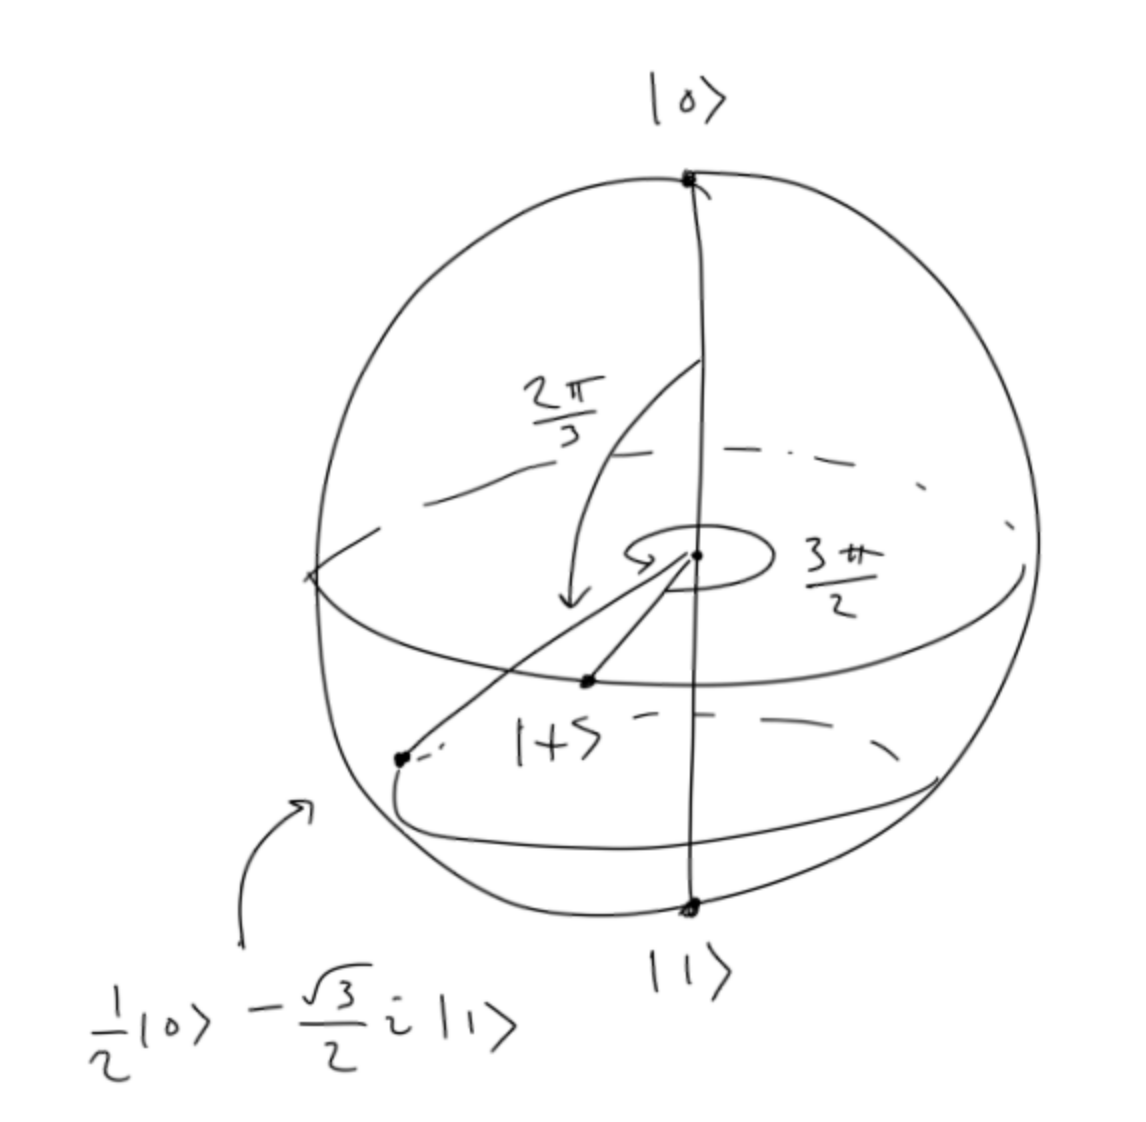
\includegraphics[width=0.8\textwidth]{review8blochsphere.png}
	\end{center}
	\caption{Bloch sphere as corresponding to $\CC \cup \{ \infty \}$ \KS{TODO: check image}}
\label{fig:bloch-wrap}
\end{figure}

The set of \emph{normalized} states can be visualized as a sphere.  Every normalized state can be written as
\[
	| \phi \rangle = 
	\cos\left( \frac{\theta}{2} \right) | 0 \rangle
	+ 
	e^{i \varphi}
	\sin\left( \frac{\theta}{2} \right) | 1 \rangle
\]
In Figure~\ref{fig:bloch} we see how these two parameters $0 \le \theta \le 2\pi$ and $0 \le \varphi \le 2\pi$ parametrize a sphere.

\begin{figure}
	\begin{center}
%		\includegraphics[width=0.8\textwidth]{bloch.png}
	\end{center}
	\caption{General Bloch sphere}
\label{fig:bloch}
\end{figure}

\KS{move this?}
Then \textbf{relative phase} is the angle the complex number $b/a$ makes with the real axis, i.e. $\varphi$.  The \textbf{relative magnitude} is the length of the complex number $b/a$, i.e. $\sin \frac{\theta}{2} / \cos \frac{\theta}{2}$. \KS{Fixed by AI: with the state $\cos(\theta/2)\,|0\rangle+e^{i\varphi}\sin(\theta/2)\,|1\rangle$ (so $a=\cos(\theta/2),\,b=e^{i\varphi}\sin(\theta/2)$), the ratio with phase $\varphi$ and magnitude $\tan(\theta/2)=\sin(\theta/2)/\cos(\theta/2)$ is $b/a$, not $a/b$. Corrected both occurrences.}

(As a quick concept check, if $\varphi=0$ and $\theta=0$, we get $|0 \rangle$ which has relative phase undefined and relative magnitude $0$.\KS{Fixed by AI: at $\theta=0$ the state is $\cos(0)|0\rangle+\sin(0)|1\rangle=|0\rangle$ (north pole), not $|1\rangle$; and indeed its relative magnitude $|b/a|=0$, consistent with $|0\rangle$.}\KS{more concept checks here})


\begin{quiz}
Locate $\frac{1}{\sqrt{5}}\left( |0\rangle + 2|1 \rangle \right)$ on the plane and on the sphere.  (Why do I have a normalization of $\frac{1}{\sqrt{5}}$ out front?)
Locate $\frac{1}{\sqrt{2}}\left( |0\rangle + i|1 \rangle \right)$ on the plane and on the sphere.
\end{quiz}
\begin{aisolution}
The $\frac{1}{\sqrt5}$ is there to normalize the state: with $a = \frac{1}{\sqrt5}$, $b = \frac{2}{\sqrt5}$ we get $|a|^2 + |b|^2 = \frac{1}{5} + \frac{4}{5} = 1$, so the vector has length $1$ and is a valid state.

For the first state the ratio is $b/a = 2$, a positive real number, so on the plane ($\CC\cup\{\infty\}$) it sits at the point $2$ on the real axis.  On the sphere its relative phase is $\varphi = 0$ and its relative magnitude is $\tan(\theta/2) = 2$, giving $\theta = 2\arctan 2 \approx 2.21$ rad; so it lies on the $\varphi = 0$ meridian (the great circle through $|0\rangle,|+\rangle,|1\rangle$), below the equator and toward $|1\rangle$ (since the magnitude $2 > 1$).

For the second state, $b/a = i$: this is exactly $|i\rangle$.  On the plane it is the point $i$ (unit distance up the imaginary axis), and on the sphere it is the corner $|i\rangle$ on the equator, at $(\theta,\varphi) = (\pi/2, \pi/2)$.
\end{aisolution}


The six `corners' of the Bloch sphere, thought of as projective vectors, are labelled $| 0 \rangle$, $| 1 \rangle$, $| 1 \rangle$, $| -1 \rangle$ $| i \rangle$, and $| -i \rangle$, representing slopes of $0$, $\infty$, $1$, $-1$, $i$, and $-i$ respectively.  In physics language, these are written as
\[
| 0 \rangle, | 1 \rangle, |+\rangle, |-\rangle, |i\rangle \text{ and } |-i \rangle
\]
respectively.  In terms of the basis $| 0 \rangle$, $| 1 \rangle$, these have locations on the Bloch sphere.

\newcommand\zeroket{|0 \rangle}
\newcommand\oneket{|1\rangle}
\newcommand\plusket{|+\rangle}
\newcommand\minusket{|-\rangle}
\newcommand\iket{|i\rangle}
\newcommand\miket{|-i\rangle}
\newcommand\oneroottwo{\frac{1}{\sqrt{2}}}
\newcommand\iroottwo{\frac{i}{\sqrt{2}}}

\begin{tabular}{l | l | l | l }
	state & $a\zeroket + b\oneket$ & $\begin{pmatrix}a \\ b \end{pmatrix}$ & $(\theta, \varphi)$ on Bloch sphere \\
	\hline
	$\zeroket$ & $1 \zeroket + 0 \oneket$ & $\begin{pmatrix}1 \\ 0 \end{pmatrix}$ & $(0,0)$ \\
	$\oneket$ & $0 \zeroket + 1 \oneket$ & $\begin{pmatrix}0 \\ 1 \end{pmatrix}$ & $(\pi,0)$ \\
	$\plusket$ & $\oneroottwo \zeroket + \oneroottwo \oneket$ & $\oneroottwo\begin{pmatrix}1 \\ 1 \end{pmatrix}$ & $(\pi/2,0)$ \\
	$\minusket$ & $\oneroottwo \zeroket - \oneroottwo \oneket$ & $\oneroottwo\begin{pmatrix}1 \\ -1 \end{pmatrix}$  & $(\pi/2,\pi)$ \\
	$\iket$ & $\oneroottwo \zeroket + \iroottwo \oneket$ & $\oneroottwo\begin{pmatrix}1 \\ i \end{pmatrix}$  & $(\pi/2,\pi/2)$ \\
	$\miket$ & $\oneroottwo \zeroket - \iroottwo \oneket$ & $\oneroottwo\begin{pmatrix}1 \\ -i \end{pmatrix}$ & $(\pi/2,3\pi/2)$ \\
\end{tabular}

Now, from the perspective of quantum computing, it is important to write every state in terms of a single basis.  The three most common bases are:
\begin{align*}
&| 0 \rangle, |1\rangle \\
&| + \rangle, |-\rangle \\
&| i \rangle, |-i\rangle 
\end{align*}
These are each orthonormal bases (the lines in $\CC^2$ that they represent are orthonormal).  Every other element in the space can be written as a linear combination in terms of this basis.  

\begin{example}
For example, suppose we wish to express $|0\rangle$ in the basis $|+\rangle$ and $|-\rangle$.
We need to find $a$ and $b$ so that
\[
\zeroket = a | + \rangle + b | - \rangle.
\]
i.e., in vector language
\[
\begin{pmatrix} 1 \\ 0 \end{pmatrix} =
a
 \frac{1}{\sqrt{2}}
\begin{pmatrix} 1 \\ 1 \end{pmatrix} + 
b
\frac{1}{\sqrt{2}}
\begin{pmatrix} 1 \\ -1 \end{pmatrix},
\]
We can solve this by linear algebra methods, or just by inspection.  If we inspect, we might notice that $a=b$ by reference to the second coordinate.  From the first coordinate, we therefore need to find $a$ such that $2a (1/\sqrt{2}) = 1$, i.e. $a  =\sqrt{2}/2 = 1/\sqrt{2}$.  Thus
\[
|0\rangle = \frac{1}{\sqrt{2}} | + \rangle + \frac{1}{\sqrt{2}} | - \rangle.
\]
\end{example}

\KS{copy the solution to the daily post that has coefficients $\frac{1+i}{2}$ etc. as an instructive example.}

It is possible to write all the basis elements of these three standard bases in terms of one another \KS{put a table of all of the solutions.}. 


\subsection{Bases and Change of Basis}

There are some useful states that have names:
\begin{enumerate}
	\item $|+\rangle = \frac{1}{\sqrt{2}}\left(|0\rangle + |1\rangle\right)$ 
	\item $|-\rangle = \frac{1}{\sqrt{2}}\left(|0\rangle - |1\rangle\right)$ 
	\item $|i\rangle = \frac{1}{\sqrt{2}}\left(|0\rangle +i|1\rangle\right)$ 
	\item $|-i\rangle = \frac{1}{\sqrt{2}}\left(|0\rangle -i |1\rangle\right)$
\end{enumerate}

We have been thinking of $|0\rangle$ and $|1\rangle$ as a standard basis for the vector space of quantum states of a qubit\footnote{White lie:  this vector space is actually a larger space than the space of states, since for states we enforce $|a|^2 + |b|^2=1$.}, i.e. $\CC^2$.  We might call it the \textbf{01-basis}.  Other standard choices are the \textbf{$\pm$-basis}, $|+\rangle$ and $|-\rangle$; and the \textbf{$\pm i$-basis}, $|i\rangle$ and $|-i\rangle$.

Once we have various different bases available, we might ask to change between the various bases.  That is to say, a vector in $\CC^2$ could be viewed in terms of different bases.  The state itself (the vector) doesn't change, but the way we write it down does.  

For example, the definitions above serve to write $|+\rangle, |-\rangle, |i\rangle$ and $|-i\rangle$ in terms of the $01$-basis $|0\rangle$ and $|1\rangle$.  But how might we write $|0\rangle$ and $|1\rangle$ in terms of the $\pm$-basis?  By linear algebra!  We need only use the equations $1$ and $2$ above and solve for $|0\rangle$ and $|1\rangle$.

So, adding the first two equations, we obtain
\[
\frac{2}{\sqrt{2}} |0\rangle = |+\rangle + |-\rangle.
\]
Similarly, by subtracting them, we obtain
\[
\frac{2}{\sqrt{2}} |1\rangle = |+ \rangle - |-\rangle.
\]
From these, we conclude that
\[
|0\rangle = \frac{1}{\sqrt{2}} |+\rangle + \frac{1}{\sqrt{2}} |-\rangle, \quad
|1\rangle = \frac{1}{\sqrt{2}} |+ \rangle - \frac{1}{\sqrt{2}} |-\rangle.
\]
\subsection{Measurement}

A qubit state cannot be directly observed.  Instead, we are only able to \textbf{measure with respect to a basis}.  This has two unexpected effects (at least from the perspective of someone used to classical measurement, such as length with a ruler):  first, we only get incomplete probabilistic information; and second, we irrevocably change the state, losing information.

The rules for measurement are as follows:  given a state
\[
a | 0 \rangle + b | 1 \rangle,
\]
if we measure in the basis $|0 \rangle$, $|1 \rangle$, then we obtain one of two answers: $|0\rangle$ or $|1 \rangle$.  The probability of obtaining the first is $|a|^2$ and the probability of obtaining the second is $|b|^2$.  Let's display this in a table:
\begin{centering}

\begin{tabular}{cc}
result & probability \\
\hline
$|0\rangle$ & $|a|^2$ \\
$|1\rangle$ & $|b|^2$ \\
\end{tabular}

\end{centering}

These probabilities add to $1$, as they must (if they are to be probabilities), because of our convention that qubit states are written so that $|a|^2 + |b|^2 = 1$.

If we measure using a different (orthonormal) basis, we will obtain one of \emph{those} basis elements as the result.  For example, using Table~\ref{table:qubit-bass} \KS{make a table of qubit bases change of bases}, the same state above can be expressed in the $|+\rangle$, $|-\rangle$ basis as follows:
\[
a | 0 \rangle + b | 1 \rangle = 
a\left(  \frac{1}{\sqrt{2} }|+\rangle + \frac{1}{\sqrt{2}} |-\rangle \right) +
b\left(  \frac{1}{\sqrt{2} }|+\rangle - \frac{1}{\sqrt{2}} |-\rangle \right)
=
\frac{a+b}{\sqrt{2}} |+\rangle + 
\frac{a-b}{\sqrt{2}} |-\rangle.
\]
Now, the probabilities for a measurement in the $|+\rangle$, $|-\rangle$ basis are given by the following table:
\begin{centering}

\begin{tabular}{cc}
result & probability \\
\hline
$|+\rangle$ & $|a+b|^2/2$ \\
$|-\rangle$ & $|a-b|^2/2$ \\
\end{tabular}

\end{centering}

It is reassuring to compute that these probabilities add to $1$:
\[
\frac{1}{2} \left(
|a+b|^2 + |a-b|^2
\right)
=
\frac{1}{2} \left(
(a_1+b_1)^2 + (a_2 + b_2)^2 + (a_1 - b_1)^2 + (a_2 - b_2)^2
\right)
=
\frac{2}{2} \left(
a_1^2+b_1^2 + a_2^2 + b_2^2
\right)
=
|a|^2 + |b|^2
=1.
\]

\subsection{Practice problems}

\begin{question}
Consider the qubit state superposition $i|0\rangle + \sqrt{3}|1 \rangle$.
\begin{enumerate}
    \item Normalize it so that it is length 1 (i.e. $|a|^2 + |b|^2 = 1$).
\item Normalize it further so that it also lies on the Bloch sphere (first entry $a$ should be positive real).
\item Find $\theta$ and $\varphi$ giving this state as a point on the Bloch sphere.
\item Draw it on a Bloch sphere.
\end{enumerate}
\end{question}

\begin{solution}
    \begin{enumerate}
        \item Right now, the state satisfies
        \[
        |a|^2 + |b|^2 = |i|^2 + |\sqrt{3}|^2 = 1^2 + 3 = 4.
        \]
        We will scale it by a complex number $\alpha$ so that this becomes $1$, i.e.
        \[
        |\alpha a|^2 + |\alpha b|^2 = 1.
        \]
        But that means we need $|\alpha|^2 = \frac{1}{4}$.  So we can scale by $\alpha = \frac{1}{2}$, so our state becomes
        \[
        \frac{i}{2} \zeroket + \frac{\sqrt{3}}{2} \oneket.
        \]
        Let's double check it worked.  This has length
        \[
        |a|^2 + |b|^2 = \frac{1}{4} + \frac{3}{4} = 1.
        \]
        \item Now, the first entry is $\frac{i}{2}$.  We would like it to be positive real, so we scale by a unit length complex number $\beta$ so that $\beta \frac{i}{2}$ is positive real.  Since $i$ is at angle $\pi/2$ on the unit circle, and positive real numbers lie at angle $0$, we must multiply by something at angle $-\pi/2$, that is, $\beta = -i$ will work.  Thus, the desired state is
        \[
        -i \left( \frac{i}{2} \zeroket + \frac{\sqrt{3}}{2} \oneket   \right)
        =
        \frac{1}{2} \zeroket - \frac{\sqrt{3}i}{2} \oneket
        \]

        \item Now we want to find $\theta$ and $\varphi$ so that
        \[
        \cos(\theta/2) = \frac{1}{2}, \quad
        e^{i\varphi} \sin(\theta/2) = -i \frac{\sqrt{3}}{2}.
        \]
        Taking $\theta = 2\pi/3$ solves the first equation, and plugging that into the second, we need\KS{Fixed by AI: $\cos(\theta/2)=1/2$ requires $\theta/2=\pi/3$, i.e.\ $\theta=2\pi/3$ (then $\sin(\theta/2)=\sqrt3/2$, giving $e^{i\varphi}=-i$). The value $\theta=\pi/3$ gives $\cos(\pi/6)=\sqrt3/2\neq1/2$. Cf.\ the identical computation in the Test Review section, which correctly uses $2\pi/3$.}
        \[
        e^{i\varphi} = -i
        \]
        which is $\varphi = -\pi/2$ or $3\pi/2$ (since $-i$ is at that angle on the unit circle).
        \item \KS{Image not included yet. :)}
    \end{enumerate}
\end{solution}

\begin{question} 
Write $|-\rangle$ as a linear combination of $|0\rangle$ and $|1\rangle$.
\end{question}

\begin{solution}
Because we are asking in terms of the basis $\zeroket$, $\oneket$, we can use the Bloch sphere.
    We look on the Bloch sphere, and see that $|-\rangle$ lies at the equation, so that $\theta = \pi/2$, and is opposite $|+\rangle$, so that $\varphi = \pi$.  Plugging these into the Bloch sphere formula, we have
    \[
     \cos(\theta/2) \zeroket
     + e^{i \varphi} \sin(\theta/2) \oneket
     = 
     \cos(\pi/4) \zeroket + e^{i\pi} \sin(\pi/4) \oneket
     =
     \frac{1}{\sqrt{2}} \zeroket + \frac{-1}{\sqrt{2}} \oneket.
    \]
\end{solution}


\begin{question} 
Write $|i\rangle$ as a linear combination of $|+\rangle$ and $|-\rangle$.
\end{question}

\begin{solution}

		We have the following meanings for these symbols: 
		\begin{align*}
			|i\rangle &= \frac{1}{\sqrt{2}}\begin{pmatrix} 1 \\ i \end{pmatrix}, \\
			|+\rangle &=
\frac{1}{\sqrt{2}}\begin{pmatrix} 1 \\ 1 \end{pmatrix}, \\
			|-\rangle &= 
\frac{1}{\sqrt{2}}\begin{pmatrix} 1 \\ -1 \end{pmatrix}.
		\end{align*}
		We are asked to solve for $a$ and $b$ so that
		\[
			|i\rangle = a |+ \rangle + b | - \rangle
		\]
		i.e. 
		\[
			\frac{1}{\sqrt{2}}\begin{pmatrix} 1 \\ i \end{pmatrix} =
			a \frac{1}{\sqrt{2}}\begin{pmatrix} 1 \\ 1 \end{pmatrix} +
			b \frac{1}{\sqrt{2}}\begin{pmatrix} 1 \\ -1 \end{pmatrix} =
		\]
		This is a linear system, 
		\[
			\frac{1}{\sqrt{2}}
			\begin{pmatrix}
				1 & 1 \\
				1 & -1 
			\end{pmatrix}
			\begin{pmatrix}
				a \\ b 
			\end{pmatrix}
			=
			\frac{1}{\sqrt{2}}
			\begin{pmatrix}
				1 \\
				i
			\end{pmatrix}.
		\]
		We can throw away the square roots on both sides:
		\[
			\begin{pmatrix}
				1 & 1 \\
				1 & -1 
			\end{pmatrix}
			\begin{pmatrix}
				a \\ b 
			\end{pmatrix}
			=
			\begin{pmatrix}
				1 \\
				i
			\end{pmatrix}.
		\]
		Then we can do some row reduction to solve:
		\[
			\begin{pmatrix}
				1 & 1 \\
				0 & -2
			\end{pmatrix}
			\begin{pmatrix}
				a \\ b 
			\end{pmatrix}
			=
			\begin{pmatrix}
				1 \\
				i-1
			\end{pmatrix}.
		\]
		\[
			\begin{pmatrix}
				1 & 0 \\
				0 & -2
			\end{pmatrix}
			\begin{pmatrix}
				a \\ b 
			\end{pmatrix}
			=
			\begin{pmatrix}
				\frac{1+i}{2} \\
				i-1
			\end{pmatrix}.
		\]
		\[
			\begin{pmatrix}
				1 & 0 \\
				0 & 1
			\end{pmatrix}
			\begin{pmatrix}
				a \\ b 
			\end{pmatrix}
			=
			\begin{pmatrix}
				\frac{1+i}{2} \\
				\frac{1-i}{2}
			\end{pmatrix}.
		\]
		The solution is $a = \frac{1+i}{2}$ and $b = \frac{1-i}{2}$, so the answer is
		\[
			|i\rangle = \frac{1+i}{2} |+ \rangle + \frac{1-i}{2} | - \rangle.
		\]
		This can definitely seem weird, so it is reassuring to check that 
		\[
			\left| \frac{1+i}{2} \right|^2 + \left| \frac{1-i}{2} \right|^2 =
			\left( \frac{1}{2} \right)^2 + \left( \frac{1}{2} \right)^2
			+ \left( \frac{1}{2} \right)^2 + \left( \frac{-1}{2} \right)^2 = 4 \left( \frac{1}{4} \right) = 1.
		\]


\end{solution}

\begin{question} 
Consider the state $|\psi\rangle = \frac{1}{\sqrt{5}} |0\rangle + \frac{2}{\sqrt{5}}|1\rangle$.
\begin{enumerate}
\item Measure it in the basis $|0\rangle$, $|1\rangle$.  What are the possible outcomes and their probabilities?
\item Measure it in the basis $|+\rangle$, $|-\rangle$.  What are the possible outcomes and their probabilities?  (To do this, you will first need to write $|\psi\rangle$ as a linear combination of $|+\rangle$ and $|-\rangle$.)
\end{enumerate}
\end{question}


\begin{solution}
\begin{enumerate}
	\item It is already expressed in this basis, so the outcome $|0\rangle$ occurs with probability
\[
	\left| \frac{1}{\sqrt{5}} \right|^2 = \frac{1}{5}
\]
and $|1 \rangle$ occurs with probability
\[
	\left| \frac{2}{\sqrt{5}} \right|^2 = \frac{4}{5}.
\]
(Good to check these add to $1$.)
\item We first need to express this in terms of $|+\rangle$ and $|-\rangle$.  To do so is very much like the previous questions, so we will just state the answers:
	\begin{align*}
		|0\rangle &= \frac{1}{\sqrt{2}} |+ \rangle + \frac{1}{\sqrt{2}} |- \rangle,  \\
		|1\rangle &= \frac{1}{\sqrt{2}} |+ \rangle - \frac{1}{\sqrt{2}} |- \rangle.
	\end{align*}
	Therefore, we obtain
	\[
		| \psi \rangle = \frac{1}{\sqrt{5}} \left(
		 \frac{1}{\sqrt{2}} |+ \rangle + \frac{1}{\sqrt{2}} |- \rangle  \\
			\right)
			+ \frac{2}{\sqrt{5}} \left(
		 \frac{1}{\sqrt{2}} |+ \rangle - \frac{1}{\sqrt{2}} |- \rangle
			\right)
			=
			\frac{3}{\sqrt{10}} | + \rangle + \frac{-1}{\sqrt{10}} |-\rangle.
		\]
		From this, we obtain $| + \rangle$ with probability 
		\[
			\left| \frac{3}{\sqrt{10}} \right|^2 = \frac{9}{10},
		\]
		and $| - \rangle$ with probability
		\[
			\left| \frac{-1}{\sqrt{10}} \right|^2 = \frac{1}{10}.
		\]
		Yay, these add to $1$, so we are somewhat reassured we didn't make too many errors.

	Another way to solve this is to write the original state in terms of the new basis directly, i.e.
	\[
		\frac{1}{\sqrt{5}} |0\rangle + \frac{2}{\sqrt{5}}|1\rangle = a |+ \rangle + b |- \rangle.
	\]
	This gives a system
	\[
		\begin{pmatrix}
			\frac{1}{\sqrt{5}} \\
			\frac{2}{\sqrt{5}}
		\end{pmatrix}
		=
		\frac{a}{\sqrt{2}} 
		\begin{pmatrix} 1 \\ 1 \end{pmatrix}
		+
		\frac{b}{\sqrt{2}}
		\begin{pmatrix} 1 \\ -1 \end{pmatrix}.
	\]
	Rewriting this, we have
	\[
		\frac{1}{\sqrt{2}}
		\begin{pmatrix}
			1 & 1 \\ 1 & -1 
		\end{pmatrix}
		\begin{pmatrix}
		a \\ b \end{pmatrix}
		=
		\frac{1}{\sqrt{5}}
		\begin{pmatrix}
		1 \\ 2 \end{pmatrix}
	\]
	Let's clean up the square roots a bit:
	\[
		\begin{pmatrix}
			1 & 1 \\ 1 & -1 
		\end{pmatrix}
		\begin{pmatrix}
		a \\ b \end{pmatrix}
		=
		\frac{2}{\sqrt{10}}
		\begin{pmatrix}
		1 \\ 2 \end{pmatrix}
	\]
	Therefore we can solve the simpler system below, and multiply the answer by $\frac{2}{\sqrt{10}}$:
	\[
		\begin{pmatrix}
			1 & 1 \\ 1 & -1 
		\end{pmatrix}
		\begin{pmatrix}
		a \\ b \end{pmatrix}
		=
		\begin{pmatrix}
		1 \\ 2 \end{pmatrix}
	\]
	This system has solution $a=3/2$ and $b=-1/2$, but we need to multiply the $\frac{2}{\sqrt{10}}$ again, so the real solution is $a = \frac{3}{\sqrt{10}}$ and $b = \frac{-1}{\sqrt{10}}$, as before.




\end{enumerate}

\end{solution}




\subsection{Quantum Key Distribution (BB84)}

\newcommand\upket{| \uparrow\rangle}
\newcommand\downket{| \downarrow\rangle}
\newcommand\neket{| \nearrow\rangle}
\newcommand\nwket{| \nwarrow\rangle}

In quantum key distribution, we are using photons as qubits that will be sent along a fiberoptic cable or laser or something along those lines.  The idea is to exploit the laws of physics to make it physically impossible to eavesdrop on the system without being detectable.

Before we get started, we will define two bases for photons, whose notation (arrows) is meant to invoke the \emph{polarization} of the photon:
\begin{align*}
\text{L basis:  }& |\uparrow \rangle , | \rightarrow \rangle, \\
\text{V basis:  }& | \nearrow \rangle, |\nwarrow \rangle.
\end{align*}
These bases have the following\footnote{I have ordered the bases so as to guarantee that in all relationships, the first coefficient is positive.  I am choosing representatives from the equivalence classes of $\PP^1_\RR$ pointing from the origin into the upper half plane.} relationships:
\begin{align*}
| \uparrow \rangle &= \frac{1}{\sqrt{2}} | \nearrow \rangle + \frac{1}{\sqrt{2}} | \nwarrow \rangle, \\
| \rightarrow \rangle &= \frac{1}{\sqrt{2}} | \nearrow \rangle - \frac{1}{\sqrt{2}} | \nwarrow \rangle, \\
| \nwarrow \rangle &= \frac{1}{\sqrt{2}} | \uparrow \rangle - \frac{1}{\sqrt{2}} | \rightarrow \rangle, \\\
| \nearrow \rangle &= \frac{1}{\sqrt{2}} | \uparrow \rangle + \frac{1}{\sqrt{2}} | \rightarrow \rangle.
\end{align*}
(For example, we might identify the $L$ basis with $|0\rangle$, $|1 \rangle$ and the $V$ basis with $|+\rangle$, $|-\rangle$.\KS{check this})
The really important thing about this setup is that if we measure either of the $L$ basis elements in the $V$ basis, we have a $50-50$ chance of obtaining $|\nwarrow\rangle$ or $|\nearrow\rangle$; and similarly for measuring $V$ basis elements in the $L$ basis.  The table below lists the complete the behaviour we obtain from this:
\vspace{1em}

\begin{centering}

\begin{tabular}{ccc}
photon & basis & result \\
\hline
$|\uparrow \rangle$ & L & $|\uparrow \rangle$ with probability $1$ \\
$|\rightarrow \rangle$ & L & $ |\rightarrow \rangle$ with probability $1$ \\
$|\nwarrow \rangle$ & L&  $ |\uparrow \rangle$ with probability $1/2$ and $|\rightarrow \rangle$ with probability $1/2$ \\
$|\nearrow \rangle$ & L&  $ |\uparrow \rangle$ with probability $1/2$ and $|\rightarrow \rangle$ with probability $1/2$ \\
$|\uparrow \rangle$ & V & $|\nwarrow \rangle$ with probability $1/2$ and $|\nearrow \rangle$ with probability $1/2$\\
$|\rightarrow \rangle$ & V & $|\nwarrow \rangle$ with probability $1/2$ and $|\nearrow \rangle$ with probability $1/2$ \\
$|\nwarrow \rangle$ & V & $ |\nwarrow \rangle$ with probability $1$ \\
$|\nearrow \rangle$ & V & $ |\nearrow \rangle$ with probability $1$ \\
\end{tabular}

\end{centering}
\vspace{1em}

The key distribution exploits the properties described in the table above.  The process is as follows, occurring in three phases:\\

\textbf{Phase I (quantum channel):}

\begin{enumerate}
\item Alice chooses a series of $n$ random bits (each is $0$ or $1$).  This is secret.
\item Alice chooses a series of $n$ random bases (each is L or V).  This is secret.
\item Bob chooses a series of $n$ random bases (each is L or V).  This is secret.
\item For each pair of bit with basis, Alice creates a photon according to the chart below, and sends it to Bob:
%\vspace{1em}
%
%\begin{centering}
%\begin{tabular}{ccc}
%bit & basis & photon \\
%\hline
%0 & L & $|\uparrow \rangle$ \\ 
%1 & L &$|\rightarrow \rangle$ \\
%0 & V & $|\nwarrow \rangle$ \\
%1 & V & $|\nearrow \rangle$ 
%\end{tabular}
%\end{centering}
%\vspace{1em}
%
%Here's a different way to display the same info:

\vspace{1em}

\begin{centering}

\begin{tabular}{c|cc}
 & 0 & 1 \\
\hline
L & $|\uparrow \rangle$ & $|\rightarrow \rangle$ \\ 
V & $|\nwarrow \rangle$ & $|\nearrow \rangle$ 
\end{tabular}

\end{centering}
\vspace{1em}

    \item Bob measures each incoming photon in order using the bases in his list.  The result is given according to the table further up this page.  The resulting photon is read as being a $0$ or $1$ according to the small table of the last step.  Bob records these bits.
    \end{enumerate}
    \textbf{Phase II (classical channel):}
    \begin{enumerate}
    \item   After the sending and measuring is done, Bob and Alice talk over an insecure channel (e.g. a phone call) and compare their lists of bases (no longer secret).  For each photon for which their bases \emph{agreed}, they keep that bit.  They discard all bits for which their bases \emph{disagreed}.
        \end{enumerate}
        \textbf{Phase III (classical channel):}
    \begin{enumerate}
    \item  To make sure there was no eavesdropping on the photon channel, they reveal (over the classical channel) and compare a small number of \emph{sample bits}.  These bits are then discarded.  
    \item If all the sample bits agreed, they keep the remaining bits as the shared secret.  
    \item If any of the sample bits disagreed, this means the quantum channel was compromised, so they throw all their work away and must begin again.
    \end{enumerate}

An example is shown in the following table.  
\vspace{1em}

\begin{centering}

\begin{tabular}{ccccccc}
Alice bit & Alice basis & photon sent & Bob basis & photon measured & bit derived & kept? \\
\hline
0 & L & $| \uparrow \rangle$ & L & $| \uparrow \rangle$ & 0 & keep \\
1 & V & $| \nearrow \rangle$ & L & $| \uparrow \rangle$ or $| \rightarrow \rangle$ & 0 or 1 & toss \\
0 & V & $| \nwarrow \rangle$ & V & $| \nwarrow \rangle$ & 0 & keep \\
1 & L & $| \rightarrow \rangle$ & V & $| \nwarrow \rangle$ or $| \nearrow \rangle$ & 0 or 1 & toss\\
1 & V & $| \nearrow \rangle$ & L & $| \uparrow \rangle$ or $| \rightarrow \rangle$ & 0 or 1 & toss\\
0 & V & $| \nwarrow \rangle$ & V & $| \nwarrow \rangle$ & 0  & keep\\
1 & L & $| \rightarrow \rangle$ & L & $| \rightarrow \rangle$ & 1 & keep\\
\end{tabular}

\end{centering}
\vspace{1em}

For example, the first row results from the following interaction.  The first photon Alice generates is based on a bit of $0$ and a basis of $L$:  therefore it is $| \uparrow \rangle$.  Bob measures it in basis $L$, so he receives it correctly as $| \uparrow \rangle$ with probability $1$.  He decodes this as a bit of $0$.

In the second row, Bob reads the photon $| \nearrow \rangle$ in the $L$ basis, so he has a 50-50 chance of getting either result and either bit.

Later, after the process is completed, Alice and Bob compare their bases and keep the photons which were sent and received in the same bases.   This is shown in the last column.  Notice that it has the effect of keeping the reliable bits and throwing out the unreliable ones.  In this example, their shared secret is $0001$.

In the final phase, they may use a few of these bits to check whether there was an eavesdropper.  More detail about that follows.


\subsubsection{The security of Quantum Key Exchange}

The security guarantee of QKD is very different from the other systems we have studied.  Here, we rely on the physical laws of quantum physics to guarantee (with overwhelming probability, anyway) that an eavesdropper can be \emph{detected}.  If an eavesdropper is detected, we simply give up and perhaps start over.

To see that Phase III detects an eavesdropper with some probability, consider what happens in the following two cases.  In both cases, imagine that we are in the first row of the example table above.  That is, Alice sends 0 in the L basis, meaning $| \uparrow \rangle$, and Bob measures the photon in the L basis.  If no eavesdropper is on the channel, Bob will measure a 0.\KS{Fixed by AI: Alice sent bit $0$ ($|\uparrow\rangle$); Bob measuring in the L basis recovers $|\uparrow\rangle$ with probability $1$, which decodes to $0$, not $1$.}

However, if there is an eavesdropper on the channel, say Eve, then she cannot interact with the photon without measuring it.  Let's consider two possibilities:

\begin{enumerate}
    \item If she measures it with the L basis, namely the basis used by both Alice and Bob, then her measurement results in $| \uparrow \rangle$ with probability 1.  In other words, she doesn't change the photon, and her examination goes undetected, since nothing about Alice or Bob's experience changes.
    \item If she measures it with the V basis, then her measurement will collapse the photon to either $| \nwarrow \rangle$ or $| \nearrow \rangle$ with equal probability.  Then, when Bob measures in the L basis, he will measure 0 or 1 with equal probability.  Thus Bob's measurement has a 50\% probability of being wrong.  If Alice and Bob proceed as in Phase II, and the measurement is wrong, their secret bitstring will differ in this position, but they won't know that.
\end{enumerate}

In order to detect Eve, Alice and Bob in Phase III will compare a small number of sample bits.  If we are in the second situation just described and Bob's measurement does not match what Alice sent, then this will be noticed, and it will tip off Alice and Bob that something is wrong with their quantum channel.

Thus, the security guarantee for this system depends on Phase III.  The level of confidence we can have that the quantum channel is secure depends on how many sample bits we compare.

From the description above, if we assume Alice is using bases L and V randomly, then there is a 3/4 chance that she gets away with it, since she is only caught when she uses a mismatched bases (1/2 probability) and it affects Bob's bit (1/2 probability).  Thus each bit we check has a 3/4 chance of letting Alice get away with it.  But if we check $k$ bits, there's only a $(3/4)^k$ chance Alice gets away with it.  As $k$ increases, this probability decreases. Thus we tune $k$ to our required level of confidence.

There are many many real-world considerations that get in the way of this nice mathematical system.  Some of them are:

\begin{enumerate}
    \item Alice could check with other bases.
    \item In practice engineering constraints require us to send groups of photons, not single photons.
    \item Someone could shine a flashlight up the line to see what polarizer (basis) Bob is using.
    \item The system has some noise in it that must be accounted for.
    \item Eve may not eavesdrop throughout the entire Phase I, but only on some of the bits
    \item Whether our bitstring must be entirely uncompromised or can allow for the leakage of a few bits depends on how it used after it is obtained.
    \item etc.
\end{enumerate}

However, this technology has been in commercial use since 2004.






\subsection{Two qubit systems}

Let us now turn to the case of two qubits.  The classical states in this case are 
\[
00, 01, 10, 11.
\]
The state of a 2-qubit system is a superposition of these four states.  That is, a 2-qubit system is in a state of the form
\[
|\psi\rangle =
\alpha_{00} | 00 \rangle
+ 
\alpha_{01} | 01 \rangle
+
\alpha_{10} | 10 \rangle
+
\alpha_{11} | 11 \rangle
\]
where $\alpha_{ij} \in \CC$, and $|\alpha_{00}|^2+|\alpha_{01}|^2+|\alpha_{10}|^2+|\alpha_{11}|^2 = 1$.  Just as in the one-qubit case, if we measure the state with respect to the basis
\[
|00 \rangle, 
|01 \rangle,
|10 \rangle, 
|11 \rangle, 
\]
then we obtain one of these results.  The table below shows the probabilities:
\vspace{1em}

\begin{centering}

\begin{tabular}{cccc}
result & probability & state after measurement \\
\hline
$00$ & $|\alpha_{00}|^2$ & $|00 \rangle$ \\
$01$ & $|\alpha_{01}|^2$ & $|01 \rangle$ \\
$10$ & $|\alpha_{10}|^2$ & $|10 \rangle$ \\
$11$ & $|\alpha_{11}|^2$ & $|11 \rangle$ \\
\end{tabular}

\end{centering}
\vspace{1em}

So far the story is just like the story for a single qubit.

But now, suppose instead we measure only one of the two qubits, say the first one (left one).  Then, we have the following results:
\vspace{1em}

\begin{centering}

\begin{tabular}{cccc}
result & probability & state after measurement \\
\hline
$0$ & $|\alpha_{00}|^2+|\alpha_{01}|^2$ & $\frac{1}{\sqrt{|\alpha_{00}|^2+|\alpha_{01}|^2}}\left(\alpha_{00}|00 \rangle+\alpha_{01}|01 \rangle\right)$ \\
$1$ & $|\alpha_{10}|^2+|\alpha_{11}|^2$ & $\frac{1}{\sqrt{|\alpha_{10}|^2+|\alpha_{11}|^2}}\left(\alpha_{10}|10 \rangle+\alpha_{11}|11 \rangle\right)$ \\
\end{tabular}

\end{centering}
\vspace{1em}

What we observe is that measuring the first qubit collapses the first qubit, so that if we measure a $0$, then the resulting state is a superposition of only $|00\rangle$ and $|01\rangle$.  In effect, we erase the other states $|10\rangle$ and $|11\rangle$ (which are now impossible) and renormalize the state to make it length $1$ (which results in the complicated factor out front).

Now suppose that after this, we measure the 2nd qubit.  Supposing the first qubit measured as a $0$, the state we are measuring is 
\[
\frac{1}{\sqrt{|\alpha_{00}|^2+|\alpha_{01}|^2}}\left(\alpha_{00}|00 \rangle+\alpha_{01}|01 \rangle\right)
\]
The probability of measuring a $0$ in the second qubit is therefore the squared norm of the first coefficient, namely
\[
|\alpha_{00}|^2\frac{1}{|\alpha_{00}|^2+|\alpha_{01}|^2}.
\]
Now, the overall probability of having the outcome $00$ is given by the product of our probabilities, i.e. 
\[
\left(|\alpha_{00}|^2+|\alpha_{01}|^2 \right) \cdot |\alpha_{00}|^2\frac{1}{|\alpha_{00}|^2+|\alpha_{01}|^2}
= |\alpha_{00}|^2.
\]
This is the same probability that we obtained when measuring both qubits simultaneously!

To summarise this situation, we have the following table:

\vspace{1em}

\begin{centering}

\begin{tabular}{cccccc}
qubit 1 & qubit 2 & prob. of 2nd result conditional on 1st & probability & resulting state \\
\hline
$0$ & $0$ &  $|\alpha_{00}|^2\frac{1}{|\alpha_{00}|^2+|\alpha_{01}|^2}$ & $|\alpha_{00}|^2$ & $|00\rangle$ \\
$0$ & $1$ &  $|\alpha_{01}|^2\frac{1}{|\alpha_{00}|^2+|\alpha_{01}|^2}$ & $|\alpha_{01}|^2$ & $|01\rangle$ \\
$1$ & $0$ &  $|\alpha_{10}|^2\frac{1}{|\alpha_{10}|^2+|\alpha_{11}|^2}$ & $|\alpha_{10}|^2$ & $|10\rangle$ \\
$1$ & $1$ &  $|\alpha_{11}|^2\frac{1}{|\alpha_{10}|^2+|\alpha_{11}|^2}$ & $|\alpha_{11}|^2$ & $|11\rangle$ \\
\end{tabular}

\end{centering}
\vspace{1em}

To summarize, we observe that the order in which we measure the qubits doesn't matter, in terms of the final probabilities.

\subsection{Quantum entanglement}

When we have multiple qubits, the joint state (as discussed above) may be either entangled or unentangled, with respect to a choice of basis.  Most of the states we might write down are entangled, but we say they are \emph{unentangled} if they behave `independently' of one another in the following sense.

Suppose first that we have two unrelated one-qubit systems, namely,
\[
|\psi_1\rangle = a_1 \zeroket + b_1 \oneket, \quad
|\psi_2\rangle = a_2 \zeroket + b_2 \oneket.
\]
Then, if I measure the first qubit, it doesn't affect the second qubit's state.

Now suppose I have a two-qubit system in the state
\[
|\psi \rangle =
a_1a_2 |00\rangle+
a_1b_2 |01\rangle+
b_1a_2 |10\rangle+
b_1b_2 |11\rangle.
\]

Then, if I measure the 1st qubit, I end up with the following:
\vspace{1em}

\begin{centering}

\begin{tabular}{cccc}
result & probability & state after measurement \\
\hline
$0$ & $|a_1|^2$ & $a_2|00 \rangle + b_2|01\rangle$ \\
$1$ & $|b_1|^2$ & $a_2|10 \rangle + b_2|11\rangle$ \\
\end{tabular}

\end{centering}
\vspace{1em}

So, effectively, measuring the first qubit didn't affect the resulting second qubit superposition.  In particular, if I now measure the 2nd qubit, I have the same relative probabilities of $0$ or $1$ in both cases (both lines of the table).

So this type of two-qubit system can be thought of as equivalent, in terms of its behaviour, to two unrelated one-qubit systems.

\begin{definition}
    A $2$-qubit state
\[
|\psi \rangle =
\alpha_{00} |00\rangle+
\alpha_{01} |01\rangle+
\alpha_{10} |10\rangle+
\alpha_{11} |11\rangle
\]
is \emph{not entangled} if it is a product of pure states:
\[
\alpha_{00} |00\rangle+
\alpha_{01} |01\rangle+
\alpha_{10} |10\rangle+
\alpha_{11} |11\rangle
=
\left(
a_1|0\rangle + b_1|1\rangle
\right)
\left(
a_2|0\rangle + b_2|1\rangle
\right)
\]
Otherwise it is \emph{entangled}.
\end{definition}

Equivalently, the state above is \emph{not entangled} if there is a solution $a_1,a_2,b_1,b_2$ to the system of equations
\[
a_1a_2 = \alpha_{00},\quad
a_1b_2 = \alpha_{01},\quad
b_1a_2 = \alpha_{10},\quad
b_1b_2 = \alpha_{11}.
\]
A slick way to prove such a system has no solutions is to check if
\[
\alpha_{00} \alpha_{11} - \alpha_{01}\alpha_{10} = 0.
\]
If it doesn't come out to zero, it must be entangled.  (Convince yourself of this!)






An example of an entangled system is the \textbf{Bell state}
\[
\frac{1}{\sqrt{2}} |00 \rangle +
\frac{1}{\sqrt{2}} |11 \rangle
\]
In this state, if I measure the 1st qubit, and obtain a $0$, then the second qubit will measure as a $0$ also.  And conversely, if I measure the 1st qubit, and obtain a $1$, then the second qubit will measure as a $1$ also. 

\begin{quiz}
Prove what I just said.  That is, work out the table of probabilities and states after measuring the first qubit, and then after measuring the second qubit, like in the last section.
\end{quiz}
\begin{aisolution}
Write the Bell state with amplitudes $\alpha_{00} = \alpha_{11} = \frac{1}{\sqrt2}$ and $\alpha_{01} = \alpha_{10} = 0$.

\emph{Measuring the first qubit.}  The probability of outcome $0$ is $|\alpha_{00}|^2 + |\alpha_{01}|^2 = \frac12 + 0 = \frac12$, and the collapsed (renormalized) state is $|00\rangle$, so the second qubit is then certainly $0$.  The probability of outcome $1$ is $|\alpha_{10}|^2 + |\alpha_{11}|^2 = 0 + \frac12 = \frac12$, and the collapsed state is $|11\rangle$, so the second qubit is certainly $1$.

\emph{Measuring the second qubit.}  By the symmetry of the state, outcome $0$ has probability $\frac12$ and collapses to $|00\rangle$ (first qubit certainly $0$), and outcome $1$ has probability $\frac12$ and collapses to $|11\rangle$ (first qubit certainly $1$).

In every case the two qubits agree, which is exactly the claimed perfect correlation.
\end{aisolution}

To check that this state is entangled, we could try to solve the system of equations
\[
\frac{1}{\sqrt{2}} = a_1a_2, \quad
0 = a_1b_2, \quad
0 = b_1a_2,\quad
\frac{1}{\sqrt{2}} = b_1b_2.
\]
This has no solution.  

\begin{remark}
    In practice, entanglement that affects the probabilities on the second qubit is very useful.  But the definition of entanglement -- not being a product of pure states -- is not actually equivalent to the statement that the probabilities are independent.  Take for example,
    \[
    \frac{1}{2} \left( 
    |00 \rangle + 
    |01 \rangle + 
    |10 \rangle +
    i|11 \rangle
    \right)
    \]
    If we measure a $0$ in the first qubit, the resulting collapsed state is
    \[
    \frac{1}{\sqrt{2}} \left(
    |00 \rangle + |01 \rangle
    \right).
    \]
    However, if we measure a $1$ in the first qubit, the resulting collapsed state is
    \[
    \frac{1}{\sqrt{2}} \left(
    |00 \rangle + i|01 \rangle
    \right).
    \]
    These two states result in the \emph{same probabilities} for the second qubit.  However, this state IS entangled, because if it were not, then we would have a solution to\KS{Fixed by AI: the point of this remark is precisely that independent second-qubit probabilities do NOT imply unentangled; the derivation below yields a contradiction, so the state IS entangled (as the last sentence also concludes). Changed ``is NOT entangled, because if it were'' to ``IS entangled, because if it were not''.}
    \[
    ac = 1, ad = 1, bc = 1, bd = i.
    \]
    But then
    \[
    i = (ac)(bd) = (ad)(bc) = 1,
    \]
    a contradiction.  So these are \emph{entangled}.
\end{remark}


\KS{Include Ekert 91 QKD with entanglement which uses Bell state}

\subsection{Quantum Entanglement Exercises}

	Here is a 2-qubit state:
		\[
			\ket{\Psi} = \frac{1}{\sqrt{2}}\ket{00} + \frac{1}{2}\ket{01} + \frac{1}{2}\ket{11}.
		\]

\begin{enumerate}
	\item Suppose you measure the first qubit and obtain a measurement of $\ket{0}$.  
		\begin{enumerate}
			\item What is the state after this measurement?
				\vspace{1em}

				\emph{Solution}

				The classical state $\ket{11}$ drops off, and we obtain, after normalizing by the length
				\[
					\frac{2}{\sqrt{3}} \left(	\frac{1}{\sqrt{2}}\ket{00} + \frac{1}{2}\ket{01} \right)
					=
					\frac{\sqrt{2}}{\sqrt{3}}\ket{00} + \frac{1}{\sqrt{3}}\ket{01}.
				\]


			\item If you now measure the second qubit, what are the possible results and probabilities of those results?
				\vspace{1em}

				\emph{Solution}

				We have probability $2/3$ that we obtain $00$ and probability $1/3$ that we obtain $01$.

				Fortunately, these add up to $1$ (always a good check to do).

		\end{enumerate}
	\item Suppose instead you measure the first qubit and obtain a measurement of $\ket{1}$.
		\begin{enumerate}
			\item What is the state after this measurement?
				\vspace{1em}

				\emph{Solution}

				The classical state $\ket{11}$ is the only one surviving, and we obtain, after normalizing by the length
				\[
					\ket{11}.
				\]


			\item If you now measure the second qubit, what are the possible results and probabilities of those results?
				\vspace{1em}

				\emph{Solution}

				We have probability $1$ that we obtain $11$.

		\end{enumerate}
	\item Is this an entangled state?  Justify.

		\emph{Solution}

		Yes.  

		One way to see this is that in the two different outcomes to measuring the first qubit, we get differing probabilities for the outcome of the second.  Hence they are not independent.

		Another way to see this is to try to solve the system of equations that would give rise to the 2-qubit amplitudes as a result of two single-qubit states:
		\[
			\frac{1}{\sqrt{2}} = a_1a_2, \quad \frac{1}{2} = a_1b_2, \quad 0 = b_1a_2 \quad \frac{1}{2} = b_1b_2.
		\]
		But this is harder in general (here it's not bad at all).


\item 	Suppose you have $n+1$ qubits.  We will write $\ket{\vec{x}}$ to mean the $n$-qubit classical state given by the number $x$ in binary.  So for example, if $n=2$ then $\ket{\vec{0}} = \ket{00}$, $\ket{\vec{3}} = \ket{11}$ etc.  Suppose the qubits are in this state:
		\[
			\ket{\Phi} =	\frac{1}{\sqrt{2^n}} \sum_{x=0}^{2^n-1} \ket{\vec{x}}\ket{x \mod 2}
		\]

\begin{enumerate}
	\item What is the resulting state if we measure the last qubit and obtain $\ket{0}$?  Make sure you have normalized your state.

		\emph{Solution}

		All the states with last qubit $\ket{1}$ disappear from the summation.  That leaves exactly half of them, i.e. those where $x$ is even.  Therefore we have
\[
	\frac{1}{\sqrt{2^{n-1}}} \sum_{x=0}^{2^{n-1}-1} \ket{\overrightarrow{2x}}\ket{0}.
		\]
 Notice that the length of the vector has changed (it has half as many non-zero entries), so the scalar out front has altered.  That's the normalization.


	\item What is the resulting state if we measure the last qubit and obtain $\ket{1}$?  Make sure you have normalized your state.

	
		\emph{Solution}
		All the states with last qubit $\ket{0}$ disappear from the summation.  That leaves exactly half of them, i.e. those where $x$ is odd.  Therefore we have
\[
	\frac{1}{\sqrt{2^{n-1}}} \sum_{x=0}^{2^{n-1}-1} \ket{\overrightarrow{2x+1}}\ket{1}.
		\]


\end{enumerate}

\item Can you measure the first qubit of the state $\frac{1}{\sqrt{2}} |00 \rangle + \frac{1}{\sqrt{2}}|01 \rangle$ and get $1$?

\emph{Solution.}
No, you cannot.  None of the classical states with non-zero coefficients have a $1$ in the left (first) position.

\item Consider the quantum state $\frac{1}{2} |00 \rangle + \frac{1}{2} |01 \rangle + \frac{1}{2} |10 \rangle + \frac{1}{2} |11 \rangle$. Is this entangled?

\emph{Solution.}  No, this is the result of the following multiplication:
\[
\left(
\frac{1}{\sqrt{2}} |0 \rangle 
+ \frac{1}{\sqrt{2}} |1 \rangle
\right)
\left(
 \frac{1}{\sqrt{2}} |0 \rangle + \frac{1}{\sqrt{2}} |1 \rangle
\right)
\]
Another way to discover this is to consider the resulting state after measuring the first qubit, supposing it was a $0$ and supposing it was a $1$.  In both cases you end up with the same collapsed state.

\item Measure the quantum state $\frac{2}{\sqrt{7}} |00 \rangle + \frac{1}{\sqrt{7}} |01 \rangle + \frac{1}{\sqrt{7}} |10 \rangle + \frac{1}{\sqrt{7}} |11 \rangle$ in the first coordinate.  What are the probabilities of the possible results, and the resulting quantum states?

\emph{Solution.}  If we measure in the first coordinate, we may end up with a zero, with probability
\[
\left| \frac{2}{\sqrt{7}} \right|^2 + 
\left| \frac{1}{\sqrt{7}} \right|^2 = \frac{5}{7}
\]
and a one, with probability
\[
\left| \frac{1}{\sqrt{7}} \right|^2 + 
\left| \frac{1}{\sqrt{7}} \right|^2 = \frac{2}{7}.
\]

In the first case, the resulting collapsed state is the normalization of the state obtained by dropping the terms with $1$ in the first qubit,
\[
\frac{2}{\sqrt{7}} |00 \rangle + \frac{1}{\sqrt{7}} |01 \rangle,
\]
namely, after normalization,
\[
\frac{2}{\sqrt{5}} |00 \rangle + \frac{1}{\sqrt{5}} |01 \rangle,
\]

Similarly, if we measured a $1$, then the resulting state is
\[
\frac{1}{\sqrt{2}} |10 \rangle + \frac{1}{\sqrt{2}} |11 \rangle
\]

\end{enumerate}




\subsection{Quantum gates}

In classical computing, we work with \emph{bits} and \emph{gates}.  Bits can take on exactly two values, one at any given time.  Gates take input bits and produce output bits.  For example, the NOT, AND and NAND gates are as follows:
\KS{input/output tables}

In quantum computing, we work with \textbf{qubits} and \textbf{quantum gates}.  We have already studied qubits:  they have a continuous state space which can be expressed in the classical basis states $|0\rangle$ and $|1 \rangle$.  Physical experiment indicates that quantum states evolve in time by unitary transformation.  A matrix U is \textbf{unitary} if $U U^\dagger = I = U^\dagger U$ where $U^\dagger$ is the conjugate transpose of $U$.

The conjugate transpose is computed by taking the transpose and applying complex conjugation to the entries.  For example,
\[
\begin{pmatrix}
a & b \\ c & d
\end{pmatrix}^\dagger
=
\begin{pmatrix}
\overline{a} & \overline{c} \\ \overline{b} & \overline{d}
\end{pmatrix}
\]
In geometric terms, $U$ is unitary if it preserves the complex length of vectors as a linear transformation, i.e.
\[
|U \mathbf{v} | = |\mathbf{v}|, \quad \forall \mathbf{v} \in \CC^n.
\]
(Note that the complex length of a vector $(v_1,\ldots,v_n)$ is $\sqrt{ |v_1|^2 + \cdots + |v_n|^2 }$.)

We will now give some simple examples of unitary matrices.  Each of these can be interpreted as a transformation on a single qubit in the basis $|0\rangle$, $|1\rangle$.

As a first example, consider the matrix
\[
\begin{pmatrix}
0 & 1 \\ 1 & 0
\end{pmatrix}.
\]
Its conjugate transpose is itself again, so it is unitary.  We can interpret this as acting on the basis states $|0 \rangle$ and $|1 \rangle$ as follows:
\begin{align*}
|0\rangle &\mapsto |1 \rangle, \\
|1\rangle &\mapsto |0 \rangle.
\end{align*}
This explains why it is considered a NOT gate; it is also called the Pauli X gate.

Some more examples are given in the table below:

\KS{table as in class notes showing Pauli X, Y, Z and Hadamard}


In greater generality, the one-qubit gates are $2 \times 2$ matrices which correspond to rotation of the Bloch sphere; there is a continuous space of possibilities.

In general, a \textbf{quantum gate acting on $n$ qubits} is a $2^n \times 2^n$ unitary matrix which is interpreted as acting on the state space of the $n$-qubit register.  (We use the term \textbf{register} for a collection of qubits.)

\KS{get a package that does circuit notation}

\KS{explain circuit notation}

An example of a two-qubit gate is given by the CNOT gate, which has matrix
\[
\begin{pmatrix}
1 & 0 & 0 & 0 \\
0 & 1 & 0 & 0 \\
0 & 0 & 0 & 1 \\
0 & 0 & 1 & 0
\end{pmatrix}
\]
interpreted in the basis given by $|00\rangle$, $|01\rangle$, $|10\rangle$ and $|11\rangle$.  In other words, it acts as follows:
\begin{align*}
|00\rangle &\mapsto |00 \rangle, \\
|01\rangle &\mapsto |01 \rangle,\\
|10\rangle &\mapsto |11 \rangle,\\
|11\rangle &\mapsto |10 \rangle.
\end{align*}
We visualize it with this circuit diagram:
\KS{make circuit for CNOT}
We think of the first bit as the \textbf{control bit} which determines whether to apply a NOT to the second bit, the \textbf{target bit}.  If the control bit is $0$, nothing changes; if the control bit is $1$, the second bit is switched.

\KS{Show example to generate a Bell state like in class notes}

In classical computing, the NAND gate is universal in the sense that combinations of the NAND gate can be used to create any classical program (in particular, it can be used to implement all the other usual gates like AND and OR etc.).  In quantum computing, the space of possible gates is continuous and infinite.  Our best hope is to find a small list of gates which can be used to \emph{approximate} any gate to a desired level of accuracy.  One such set is the Clifford + T gates, which consist of the one-qubit Hadamard gate, the two-qubit CNOT gate, and two other one-qubit gates:
\[
S = \begin{pmatrix}
1 & 0 \\ 0 & i
\end{pmatrix}, \quad
T = \begin{pmatrix}
1 & 0 \\ 0 & e^{i\pi/4} \end{pmatrix}
\]





\subsection{Computing classical functions}

Since unitary matrices are invertible, every quantum gate is reversible, meaning that there's a quantum gate that `undoes' it.  In particular, we cannot lose information.  However, many classical gates lose information.  An example is the AND gate, whose action is given by the following table:
\KS{make AND table}

Can we compute AND on a quantum computer?  The answer is yes, by finding an invertible transformation that has AND `inside it'.  For example, consider the following transformation on a 3-qubit register:
\begin{align*}
|000\rangle &\mapsto |000 \rangle, \\
|010\rangle &\mapsto |010 \rangle,\\
|100\rangle &\mapsto |100 \rangle,\\
|110\rangle &\mapsto |111 \rangle,\\
|001\rangle &\mapsto |001 \rangle, \\
|011\rangle &\mapsto |011 \rangle,\\
|101\rangle &\mapsto |101 \rangle,\\
|111\rangle &\mapsto |110 \rangle.
\end{align*}
You'll notice that the first two qubits $|x\rangle$ and $|y\rangle$ are unchanged, and the third qubit, if it started as $|0\rangle$, becomes $|x \wedge y \rangle$.  This part of the transformation computes AND.  The rest of the transformation is filled out to create a bijection, i.e. a reversible transformation.

To write down the matrix for this transformation, it will be an $8 \times 8$ matrix, because with $3$ qubits we have $8$ classical possibilities.  The columns of a matrix tell us where the basis elements go.  The first row of the table above says that the first column is $(1,0,0,0,0,0,0,0)$ etc.  Using the basis ordering that `counts up' in binary, i.e. 
\[
|000\rangle,
|001\rangle,
|010\rangle,
|011\rangle,
|100\rangle,
|101\rangle,
|110\rangle,
|111\rangle,
\]
the transformation swaps the last two basis vectors.  Here's the resulting matrix:
\[
\begin{pmatrix}
1 & 0 & 0 & 0 & 0 & 0 & 0 & 0  \\
0 & 1 & 0 & 0 & 0 & 0 & 0 & 0  \\
0 & 0 & 1 & 0 & 0 & 0 & 0 & 0  \\
0 & 0 & 0 & 1 & 0 & 0 & 0 & 0  \\
0 & 0 & 0 & 0 & 1 & 0 & 0 & 0  \\
0 & 0 & 0 & 0 & 0 & 1 & 0 & 0  \\
0 & 0 & 0 & 0 & 0 & 0 & 0 & 1  \\
0 & 0 & 0 & 0 & 0 & 0 & 1 & 0  \\
\end{pmatrix}
\]


This is an example of a general method for making a reversible circuit out of a general function $f$:
\[
(x,y) \mapsto (x, y XOR f(x) ).
\]

There are some details missing, but in the end, it is possible to create a quantum gate that will compute any function $f: \{ 0,1 \}^n \rightarrow \{0, 1 \}^k$ on input the states of one qubit register, and give as output the states in another qubit register, i.e. a unitary transformation that behaves as follows:
\[
| x \rangle | 0 \rangle | 0 \rangle \mapsto | x \rangle | f(x) \rangle | 0 \rangle.
\]
Note that here the first register is $n$ qubits, the second is $k$ qubits, and we are sometimes required to include some extra, or ancilla qubits to complete the task, shown here in a third register.  The mapping above doesn't tell us what the function does on inputs in which the second and third registers are not zero'ed out.  It is this freedom (to do other things on other inputs) that allows us to create a unitary (and in particular, reversible) transformation.

This capabilities is a type of `massive parallelism': with one unitary transformation, we can `compute' $f(x)$ for all $2^n$ classical inputs simultaneously!  That is (ignoring the ancillary bits):
\[
 U_f \left(
 \sum_{x \in \{0,1\}^n }
 \alpha_x | x \rangle | 0 \rangle
 \right) 
 =
 \sum_{x \in \{0,1\}^n }
 \alpha_x | x \rangle | f(x) \rangle.
\]
This sounds amazing, but there's an elephant in the room:  physics dictates that we cannot see the state we have created.  We can only measure it.  If we measure the state above (all qubits at once) we will obtain a state of the form
\[
| x \rangle | f(x) \rangle.
\]
So this is just one computation of the function $f$, not all of them.  Even worse, we can't even control which of the $x$ it computes $f(x)$ for.  In a way, it's even worse than a classical computer.

We will need one more powerful ingredient to use a state like this.  The idea is that the measurement we just tried was the `wrong' measurement.  Maybe it would be better to measure in a different basis.  But which one?

\subsection{Quantum Gates Exercises}


\begin{enumerate}


\item Apply the Pauli Y gate to the state $\frac{1}{\sqrt{5}} |0\rangle + \frac{2}{\sqrt{5}} |1 \rangle$.  What is the result?

\emph{Solution.}  The Pauli $Y$ matrix is
\[
Y = \begin{pmatrix}
    0 & -i \\ i & 0 
\end{pmatrix}
\]
so we have to evaluate
\[
\begin{pmatrix}
    0 & -i \\ i & 0 
\end{pmatrix}
\begin{pmatrix}
    \frac{1}{\sqrt{5}} \\ 
    \frac{2}{\sqrt{5}}
\end{pmatrix}
= 
\begin{pmatrix}
    \frac{-2i}{\sqrt{5}} \\ 
    \frac{i}{\sqrt{5}}
\end{pmatrix}
\]
So the resulting state is $\frac{-2i}{\sqrt{5}} |0\rangle + \frac{i}{\sqrt{5}} |1 \rangle$.


\item Check that the Hadamard gate is unitary.

\emph{Solution.}  We have
\[
H = \frac{1}{\sqrt{2}}\begin{pmatrix}
    1 & 1 \\ 1 & -1 
\end{pmatrix}
\]
We compute the conjugate transpose.  Transpose means we swap along the anti-diagonal, and conjugate means we change all $i$'s to $-i$'s (although in this case there are no changes from either of these operations).
\[
H^\dagger = \frac{1}{\sqrt{2}}\begin{pmatrix}
    1 & 1 \\ 1 & -1 
\end{pmatrix} = H.
\]
To check it is unitary, we compute
\[
H^\dagger H = H^2 = \frac{1}{{2}}
\begin{pmatrix}
    1 & 1 \\ 1 & -1 
\end{pmatrix}
\begin{pmatrix}
    1 & 1 \\ 1 & -1 
\end{pmatrix}
=
\frac{1}{2} \begin{pmatrix}
    2 & 0 \\ 0 & 2 
\end{pmatrix}
=
 \begin{pmatrix}
    1 & 0 \\ 0 & 1 
\end{pmatrix}.
\]
The fact that this came out to the identity means that, yes, it is unitary.

\item Apply the CNOT gate to the state $\frac{1}{\sqrt{5}}|00\rangle + \frac{2}{\sqrt{5}} |11 \rangle$.  What is the result?

\emph{Solution.}  The CNOT gate in terms of the basis in the usual order is 
\[
\begin{pmatrix}
1 & 0 & 0 & 0 \\
0 & 1 & 0 & 0 \\
0 & 0 & 0 & 1 \\
0 & 0 & 1 & 0
\end{pmatrix}
\]
The given state, as a vector in terms of the basis in the usual order is
\[
\begin{pmatrix}
    \frac{1}{\sqrt{5}} \\
    0 \\
    0 \\
    \frac{2}{\sqrt{5}} 
\end{pmatrix}.
\]
We multiply these and get
\[
\begin{pmatrix}
    \frac{1}{\sqrt{5}} \\
    0 \\
    \frac{2}{\sqrt{5}}  \\
    0 
\end{pmatrix}.
\]
That is, the resulting state is
$\frac{1}{\sqrt{5}}|00\rangle + \frac{2}{\sqrt{5}} |10 \rangle$.

Another way to do this problem is to apply the CNOT rule to each classical state.  CNOT flips the second bit whenever the first bit is a 1, so it changes $11$ to $10$ and leaves $00$ unchanged.

	\item Here's a new gate called the square root of not (presented in the $\ket{0}$, $\ket{1}$ basis as usual):
		\[
			\sqrt{X} = \frac{1}{2} \begin{pmatrix}
				1+i & 1-i \\
				1-i & 1+i 
			\end{pmatrix}
		\]
		Do the following:
		\begin{enumerate}
			\item Check that this gate is unitary.
			\item Check that it squares to the Pauli X or NOT gate.
			\item Figure out what $\sqrt{X}\ket{0}$ is in terms of $\ket{0}$ and $\ket{1}$.
			\item Figure out what $\sqrt{X}\ket{1}$ is in terms of $\ket{0}$ and $\ket{1}$.
		\end{enumerate}

		\emph{Solution.}
		\begin{enumerate}
			\item The conjugate transpose is
		\[
			\sqrt{X}^\dagger = \frac{1}{2}\begin{pmatrix}
				1-i & 1+i \\
				1+i & 1-i 
			\end{pmatrix}
		\]
				It is useful to compute
				\[
					(1-i)^2 = -2i, \quad (1+i)^2 = 2i, \quad (1-i)(1+i) = 2.
					\]
				We have
				\[
					\sqrt{X} \sqrt{X}^\dagger = \frac{1}{4} \begin{pmatrix}
				4 & 0 \\
				0 & 4 
					\end{pmatrix}.
					\]
					Similarly, $\sqrt{X}^\dagger \sqrt{X} = I$.

				\item We compute $\sqrt{X}^2 = X$ by matrix multiplication similarly to the last part.
				\item Since the gate is presented in the $\ket{0}$, $\ket{1}$ basis, the first column tells us where $\ket{0}$ goes, namely,
					\[
						\sqrt{X} \ket{0} =	\frac{1+i}{2} \ket{0} + \frac{1-i}{2} \ket{1}.
					\]
					Similarly,
				\[
						\sqrt{X} \ket{1} =	\frac{1-i}{2} \ket{0} + \frac{1+i}{2} \ket{1}.
						\]
		\end{enumerate}


	\item  Define a $3$-qubit gate that can be used to compute a reversible form of OR.

		\emph{Solution.}

		We use the same trick as for AND:  we use $x,y,z \mapsto x,y,z \oplus (x \vee y)$.  Then on the inputs $x,y,0$ it gives $x,y,x \vee y$.  That is, we have
\begin{align*}
|000\rangle &\mapsto |000 \rangle, \\
|010\rangle &\mapsto |011 \rangle,\\
|100\rangle &\mapsto |101 \rangle,\\
|110\rangle &\mapsto |111 \rangle,\\
|001\rangle &\mapsto |001 \rangle, \\
|011\rangle &\mapsto |010 \rangle,\\
|101\rangle &\mapsto |100 \rangle,\\
|111\rangle &\mapsto |110 \rangle.
\end{align*}
		As a matrix on the basis
		\[
			\ket{000}, \ket{001}, \ket{010}, \ket{011}, \ket{100}, \ket{101}, \ket{110}, \ket{111},
		\]
		this becomes 
		\[
			\begin{pmatrix}
				1 & 0 & 0 & 0 & 0 & 0 & 0 & 0 \\
				0 & 1 & 0 & 0 & 0 & 0 & 0 & 0 \\
				0 & 0 & 0 & 1 & 0 & 0 & 0 & 0 \\
				0 & 0 & 1 & 0 & 0 & 0 & 0 & 0 \\
				0 & 0 & 0 & 0 & 0 & 1 & 0 & 0 \\
				0 & 0 & 0 & 0 & 1 & 0 & 0 & 0 \\
				0 & 0 & 0 & 0 & 0 & 0 & 0 & 1 \\
				0 & 0 & 0 & 0 & 0 & 0 & 1 & 0
			\end{pmatrix}
		\]

			
	\item Determine a $2$-qubit quantum circuit that will, on input $\ket{00}$, produce output
		\[
			\frac{1}{2} \ket{00} + \frac{1}{2} \ket{01} + \frac{1}{2} \ket{10} + \frac{1}{2} \ket{11}.
			\]

				\emph{Solution}

				Apply a Hadamard gate to each qubit individually.  We obtain
				\[
					\left( \frac{1}{\sqrt{2}}\ket{0} + \frac{1}{\sqrt{2}}\ket{1} \right)
					\otimes \left( \frac{1}{\sqrt{2}}\ket{0} + \frac{1}{\sqrt{2}}\ket{1} \right)
					\]
					which is the state desired.  (You don't need to write the $\otimes$ in the middle, but it's common notation when we are separating qubits in a combined system.)

					Another way to solve this problem is to find a $4 \times 4$ unitary gate which has first column consisting all of the same entry (say, all $1$'s up to normalization).   There are various ways one may do this, including for example:
					\[
						\frac{1}{2}
						\begin{pmatrix}
							1 & 1 & 1 & 1 \\
							1 & i & -1 & -i \\
							1 & -1 & 1 & -1 \\
							1 & -i & -1 & i
						\end{pmatrix},
						\frac{1}{2}
						\begin{pmatrix}
							1 & 1 & 1 & 1 \\
							1 & -1 & -1 & 1 \\
							1 & -1 & 1 & -1 \\
							1 & 1 & -1 & -1
						\end{pmatrix}
					\]

					Note that these different solutions may not behave the same way on other inputs.


\end{enumerate}

More problems that don't have solutions included.

\begin{enumerate}
\item Consider the gate 
\[
S = \begin{pmatrix}
    1 & 0 \\ 0 & e^{i\pi/2}
\end{pmatrix}
\]
\begin{enumerate}
    \item Determine the conjugate transpose $S^\dagger$.
    \item Show that $S$ is unitary, hence a quantum gate.
    \item How many qubits does $S$ act upon?
    \item Apply the $S$ gate to the state $|0\rangle$.
    \item Apply the $S$ gate to the state $|+\rangle$.
    \item The gate $S^2$ is a well-known gate (one of the ones defined in the course notes).  What gate is it?
\end{enumerate}
\item Apply the reversible AND gate (as demonstrated in class, and also above in the notes) to the state
\[
			\frac{1}{2} \ket{000} + \frac{1}{2} \ket{011} + \frac{1}{2} \ket{101} + \frac{1}{2} \ket{111}.
			\]
    \item Determine a quantum circuit that will produce, from input state $|00\rangle$, the output state $\frac{1}{\sqrt{2}}|01\rangle + \frac{1}{\sqrt{2}}|10 \rangle$.
\end{enumerate}



\subsection{Roots of Unity in the Complex Numbers}

Recall that 
\[
e^{i\theta} = \cos(\theta) + i \sin(\theta).
\]
(You can think of the exponential notation as just a notation for this complex number, although there is a notion of exponentiation to complex numbers which makes sense.)
In particular, we have some useful exponent rules:
\[
e^{i \theta_1}
e^{i \theta_2}=
e^{i(\theta_1 + \theta_2)}
\]
All of these complex values are length $1$ vectors on the unit circle in the complex plane.  We use a special notation for some of them (here $m$ is a positive integer):
\[
\omega_m := e^{2 \pi i/m}.
\]
The values
\[
\omega_m, \omega_m^2, \omega_m^3, \ldots, \omega_m^{m-1}
\]
are called the $m$-th roots of unity, and they are evenly distributed around the unit circle (as if you had to cut the pie into $m$ equal slices).  Note that
\[
\omega_m^m = 1 = \omega_m^0.
\]




\subsection{Fourier transforms}

In order to discuss the fourier transform, we will consider a special vector space, the space of functions
\[
\{ f \colon \ZZ/m\ZZ \rightarrow \CC \}.
\]
Any such function can be thought of as a chart of values:
\vspace{1em}

\begin{centering}
\begin{tabular}{c|c}
$x$ & $f(x)$ \\
\hline
$0$ & $f(0)$ \\
$1$ & $f(1)$ \\
$2$ & $f(2)$ \\
$\vdots$ & $\vdots$ \\
$m-1$ & $f(m-1)$
\end{tabular}
\end{centering}

Thought of this way, it is easy to think of such a function as the vector in $\CC^m$ given by
\[
(f(0), f(1), f(2), \ldots, f(m-1) )
\]
So this space of functions is isomorphic to $\CC^m$.  If we add two functions, we are adding them coordinatewise
\KS{do example}

% >>> AI-GENERATED EXAMPLE (needs review) >>>
\begin{example}
Take $m = 4$, and let $f, g \colon \ZZ/4\ZZ \rightarrow \CC$ be the functions
\[
f = (f(0), f(1), f(2), f(3)) = (2,\ i,\ -1,\ 3), \qquad
g = (g(0), g(1), g(2), g(3)) = (1,\ 1,\ i,\ -3).
\]
Their sum $f + g$ is computed one coordinate at a time, $(f+g)(x) = f(x) + g(x)$:
\[
f + g = (2 + 1,\ i + 1,\ -1 + i,\ 3 - 3) = (3,\ 1+i,\ -1+i,\ 0).
\]
This is exactly the usual vector addition in $\CC^4$, which is why we regard the space of functions $\{f \colon \ZZ/4\ZZ \rightarrow \CC\}$ as being $\CC^4$.
\end{example}
% <<< END AI-GENERATED EXAMPLE <<<

There is a very natural standard choice of basis for these functions, which, written as vectors, looks just like the usual standard basis.  That is, $f_i$ is the function which is $1$ at $i$ and $0$ everywhere else.  Explicitly, 
There is a very natural standard choice of basis for these functions, which, written as vectors, looks just like the usual standard basis.  That is, $f_i$ is the function which is $1$ at $i$ and $0$ everywhere else.  Explicitly, 
\[
f_i(x) = \left\{
\begin{array}{ll}
1 & x = i \\
0 & \text{otherwise}
\end{array}
\right.
\]

The Fourier basis consists of functions 
\[
g_i(x) = \omega_m^{ix}.
\]
For example, when $m=3$, we have
\vspace{1em}

\begin{centering}
\begin{tabular}{c|c}
$x$ & $g_0(x)$ \\
\hline
$0$ & $1$ \\
$1$ & $1$ \\
$2$ & $1$
\end{tabular} \hfill
\begin{tabular}{c|c}
$x$ & $g_1(x)$ \\
\hline
$0$ & $1$ \\
$1$ & $\omega_3$ \\
$2$ & $\omega_3^2$
\end{tabular}
\hfill
\begin{tabular}{c|c}
$x$ & $g_2(x)$ \\
\hline
$0$ & $1$ \\
$1$ & $\omega_3^2$ \\
$2$ & $\omega_3$
\end{tabular}
\end{centering}
\vspace{1em}
\KS{fix spacing}

(Notice that in the last row of the last function, I've simplified using the rule that $\omega_3^3 = 1$, i.e. $\omega_3^4 = \omega_3$.)

These functions, if visualized, `wrap around' the axis like a helix -- see the in-class notes.


\KS{The Fourier basis -- see lecture notes for now}

\subsection{Quantum Fourier Transform}

The Quantum Fourier Transform for functions $\ZZ/m\ZZ \rightarrow \CC$ is the following linear transformation, which changes from the standard basis for functions to the frequency/Fourier basis for functions (recall the notation $\omega_m = e^{2 \pi i / m}$ from the section above on Roots of Unity). 
\[
\frac{1}{\sqrt{m}}
\begin{pmatrix}
1& 1 & 1 & 1 & \cdots & 1 \\
1 & \omega_m & \omega_m^2 & \omega_m^3 & \cdots & \omega_m^{m-1} \\
1 & \omega_m^2 & \omega_m^4 & \omega_m^6 & \cdots & \omega_m^{2(m-1)} \\
1 & \omega_m^3 & \omega_m^6 & \omega_m^9 & \cdots & \omega_m^{3(m-1)} \\
\vdots & \vdots & \vdots & \vdots & \ddots & \vdots \\
1 & \omega_m^{m-1} & \omega_m^{2(m-1)} & \omega_m^{3(m-1)} & \cdots & \omega_m^{(m-1)(m-1)} \\
\end{pmatrix}
\]
In particular, the $ij$-th entry here is $\omega_m^{ij}$.  

This matrix turns out to be unitary.  So we can think of it as a quantum gate.  

For example, for $m=2$, $\omega_2 = -1$ and the Quantum Fourier Transform is
\[
\frac{1}{\sqrt{2}}
\begin{pmatrix}
1 & 1 \\
1 & -1
\end{pmatrix}
\]
This is a single-qubit gate (a $2 \times 2$ matrix).

And for $m=4$, $\omega_4 = i$ and the QFT is
\[
\frac{1}{2}
\begin{pmatrix}
1 & 1 & 1 & 1\\
1 & i & -1 & -i \\
1 & -1 & 1 & -1 \\
1 & -i & -1 & i
\end{pmatrix}
\]
This is a 2-qubit gate (a $4 \times 4$ matrix).

Let's interpret this last matrix in quantum/dirac notation.  We will use the convention that instead of writing out binary for the classical states, we will write the binary number the string of $0$'s and $1$'s represents in decimal instead.  So the standard basis for two qubits is:
\[
|00\rangle = |0\rangle , |01 \rangle = |1\rangle , |10\rangle = |2\rangle , |11 \rangle = |3\rangle.
\]
The first column of the $4 \times 4$ QFT above tells us that
\[
|0\rangle \mapsto \frac{1}{2}\left( |0\rangle + |1\rangle + |2 \rangle + |3 \rangle \right) = \frac{1}{2}\left( \sum_{x=0}^3 |x\rangle \right).
\]
The second column tells us that
\[
|1\rangle \mapsto \frac{1}{2}\left( |0\rangle + i|1\rangle - |2 \rangle -i |3 \rangle\right) = \frac{1}{2}\left( \sum_{x=0}^3 i^x |x\rangle \right).
\]
Going on in this way, we get
\[
|k\rangle \mapsto \frac{1}{2}\left( |0\rangle + i^k |1\rangle + i^{2k} |2 \rangle + i^{3k} |3 \rangle \right) = \frac{1}{2}\left( \sum_{x=0}^3 i^{kx} |x\rangle \right).
\]

Generalizing from that example and using the matrix formula for the QFT, here is the QFT written in quantum notation on a single basis state:
\[
	|k \rangle
	\mapsto
	\frac{1}{\sqrt{m}} \sum_{x=0}^{m-1} \omega_m^{kx} |x \rangle.
\]
Then, by linearity, here it is on a general superposition of basis states:
\[
	\sum_{k=0}^{m-1} \alpha_k |k \rangle
	\mapsto
	\frac{1}{\sqrt{m}}\sum_{x=0}^{m-1} \sum_{k=0}^{m-1} \alpha_k \omega_m^{kx} |x \rangle.
\]

Now let's work out a few examples that show how the Fourier transform accomplishes its task of identifying frequencies.



Let's consider the two-qubit version again ($m=4$, $\omega_4 = i$), where the QFT is
\[
\frac{1}{2}
\begin{pmatrix}
1 & 1 & 1 & 1\\
1 & i & -1 & -i \\
1 & -1 & 1 & -1 \\
1 & -i & -1 & i
\end{pmatrix}
\]
Let's record its action on the basis states:
\begin{align*}
|00\rangle &\mapsto \frac{1}{2} \left( |00\rangle + |01 \rangle + |10 \rangle + |11 \rangle \right), \\
|01\rangle &\mapsto \frac{1}{2} \left( |00\rangle + i |01 \rangle - |10 \rangle -i |11 \rangle \right), \\
|10\rangle &\mapsto \frac{1}{2} \left( |00\rangle - |01 \rangle + |10 \rangle - |11 \rangle \right), \\
|11\rangle &\mapsto\frac{1}{2} \left(  |00\rangle -i |01 \rangle - |10 \rangle + i|11 \rangle \right).
\end{align*}
From this, we can see what happens to a uniform superposition of the states:
\[
\frac{1}{2} \left( |00\rangle + |01 \rangle + |10 \rangle + |11 \rangle  \right) \mapsto
|00\rangle.
\]
But why does this happen?  Let's take a look at each coefficient of the output.  To compute the coefficient of $|00\rangle$ in the output, we are adding up the entries of the first \emph{row} of the matrix (times 1/2).  This is because we are taking the sum of the columns (times 1/2) to create the output.

The first row of the matrix adds to $1$ because all the unit complex number entries point the same way.

The second row of the matrix adds to $0$ because the entries all point out in the four cardinal directions, cancelling.

The third row of the matrix adds to $0$ because the entries  pull equally in the positive and negative real directions.

The last row of the matrix adds to $0$ because the entries all point out in the four cardinal directions, cancelling.

\KS{Create a drawing of the cancellation in rows...}

The QFT matrix is designed in this special way to cancel out to $0$ most of the time, and just pick up special behaviour corresponding to the frequency of the input states.  The statement of this behaviour is as follows:

Let $m = 2^n$ and $r \mid m$.  Let $0 \le \ell < r$ (essentially a residue modulo $r$).  Consider an input state of the form
\[
\frac{1}{\sqrt{m/r}} \sum_{k=0}^{m/r-1} | \ell + k r \rangle.
\]
This is a state that has zero coefficients in most positions and has a positive real coefficient for those $|x \rangle$ for which $x \equiv \ell \pmod{r}$.  It looks like this: \KS{make pic}.

The QFT, applied to this state, will give an output state of the following form:
\[
\frac{1}{\sqrt{m}\sqrt{m/r}} \sum_{y=0}^{m-1} \left(
\sum_{k=0}^{m/r-1} \omega_m^{(\ell+kr)y} \right) |y\rangle.
\]
In particular, the coefficient at $|y \rangle$ is
\[
\frac{1}{\sqrt{m}\sqrt{m/r}} \sum_{k=0}^{m/r-1} \omega_m^{(\ell+kr)y}
\]
which has norm squared $1/r$ when $y \equiv 0 \pmod{m/r}$ and $0$ otherwise.  To see this, we compute in the case that $y$ is a multiple of $m/r$ that
\[
\frac{1}{\sqrt{m}\sqrt{m/r}} \sum_{k=0}^{m/r-1} \omega_m^{(\ell+kr)y}
=
\frac{1}{\sqrt{m}\sqrt{m/r}} \omega_m^\ell \sum_{k=0}^{m/r-1} \omega_m^{kry}
=
\frac{1}{\sqrt{m}\sqrt{m/r}} \omega_m^\ell \sum_{k=0}^{m/r-1} 1
=
\frac{1}{\sqrt{m}\sqrt{m/r}} \omega_m^\ell \frac{m}{r}
=
 \frac{\omega_m^\ell}{\sqrt{r}}
\]
which has magnitude squared $1/r$.

Since these $r$ magnitudes add up to $1$, all the other amplitudes/coefficients are $0$.  In practice, this happens because the sum
\[
\sum_{k=0}^{m/r-1} \omega_m^{kry}
\]
has entries distributed around the unit circle and they all cancel.

If $m/r$ is not an integer, then this is slightly messier, but we still get peaks at or near the relevant frequencies.  Specifically, let $s = \lfloor \frac{m}{r} \rfloor$.  Then we can compute the amplitude at $|y \rangle$ to be
\[
\alpha_y := \frac{1}{\sqrt{m}\sqrt{s}} \sum_{k=0}^{s-1} \omega_m^{(\ell+kr)y}
\]
Then
\[
|\alpha_y|^2 = \frac{1}{sm} \left|
\sum_{k=0}^{s-1} \omega_m^{kry}
 \right|^2
 = \frac{1}{sm} \left|
\frac{1-\omega_m^{rys}}{1 - \omega_m^{ry}}
 \right|^2
  = \frac{1}{sm} \left|
\frac{\sin\left( \frac{2 \pi r y s}{m} \right)}{\sin\left( \frac{2 \pi r y}{m} \right)}
 \right|^2
\]
This has the form
\[
  \frac{1}{sm} \left|
\frac{\sin\left( \frac{\theta s}{m} \right)}{\sin\left( \frac{\theta}{m} \right)}
 \right|^2
 \]
and it will have peaks when $\theta$ is near $2\pi \ZZ$, i.e. $y$ is near $\frac{m}{r} \ZZ$.

In other words, the output state will tend to be measured near $\frac{m}{r}$ for some $m$, i.e. multiples of the frequency $1/r$.
The offset $\ell$ is absorbed into the phase of the output state, not the magnitude of the amplitudes, so it won't be picked up by measurements.


\subsection{QFT Exercises}



\begin{enumerate}

\item Apply the $4 \times 4$ QFT matrix to the state
\[
  \frac{1}{\sqrt{2}} \left(
|00 \rangle +
\frac{1+i}{2} |01 \rangle +
\frac{1-i}{2} |11 \rangle
  \right)
\]
\item Now, notice that the state above is the (normalized) sum of the first two columns in QFT matrix.  Just using that info, explain why you could predict the result?

\item Draw the 8th roots of unity in the complex plane and label them.  You can use the $8$-th root of unity notation $\omega := \omega_8 = e^{i \pi/4}$.  But simplify it so that the labels are $\{1,-1,i,-i, \omega, -\omega, i\omega, -i\omega\}$.

\emph{Solution.}  Draw a unit circle, and mark it into 8 equal slices of pie.  The 8 tickmarks on the circle are labelled, in order counterclockwise from the real axis, 
\[
1, \omega, \omega^2, \omega^3, \omega^4, \omega^5, \omega^6, \omega^7.
\]
If we simplify some of these, we get
\[
1, \omega, \omega^2 = i, \omega^3 = i \omega, \omega^4 = -1, \omega^5 = -\omega, \omega^6 = -i, \omega^7 = -i \omega.
\]
	
			\item Write down the QFT matrix of dimension $8 \times 8$.  You can use the $8$-th root of unity notation $\omega := \omega_8 = e^{i \pi/4}$.  But simplify it so that the entries are all from the set $\{1,-1,i,-i, \omega, -\omega, i\omega, -i\omega\}$.

				\emph{Solution.}

				\[
					\frac{1}{\sqrt{8}}
					\begin{pmatrix}
						1 & 1 & 1 & 1 & 1 & 1 & 1 & 1 \\
						1 & \omega & i & i\omega & -1 & -\omega & -i & -i\omega \\
						1 & i & -1 & -i & 1 & i & -1 & -i \\
						1 & i\omega & -i & \omega & -1 & -i\omega & i & -\omega \\
						1 & -1 & 1 & -1 & 1 & -1 & 1 & -1 \\
						1 & -\omega & i & -i\omega & -1 & \omega & -i & i\omega \\
						1 & -i & -1 & i & 1 & -i & -1 & i \\
						1 & -i\omega & -i & -\omega & -1 & i\omega & i & \omega \\
					\end{pmatrix}
					\]

			\item Compute where $|3\rangle = |011\rangle$ is taken by the QFT above.

				\emph{Solution.}

				This is the 4th basis vector, so we look at the fourth column:
				\[
					\frac{1}{\sqrt{8}} \left(
					|000\rangle
					+i \omega |001\rangle
					- i |010\rangle
					 +\omega |011\rangle
					-|100\rangle
					- i \omega |101\rangle
					+ i |110\rangle
					- \omega |111\rangle
				\right)
				\]
\KS{Fixed by AI: reading the fourth column ($\omega^{3i}$) of the $8\times8$ matrix, the $|101\rangle$ ($i=5$) coefficient is $\omega^{15}=\omega^{7}=-i\omega$ and the $|111\rangle$ ($i=7$) coefficient is $\omega^{21}=\omega^{5}=-\omega$; the original had these two swapped (and they match the matrix's own $6$th row col.\ $6$).}

 
			\item The next several questions are a progression.

		\begin{enumerate}
			\item What do you get if you apply the QFT of size $m = 2^n$ to the state
				\[
					\frac{1}{\sqrt{m}}\sum_{x=0}^{m-1} \ket{x}?
				\]
			      Give the answer in the form
				\[
					\sum_{x=0}^{m-1} \alpha_x \ket{x}.
				\]
				where $\alpha_x$ is as explicit as possible.
			\item Now, with reference to the last question, what is the explicit result (compute the coefficients exactly as complex numbers) if $m = 2^2 = 4$?
			\item What about when $m=8$?
			\item What do you notice?  Conjecture what happens in general.
			\item Prove it.  (Note, there's a complex-numbers geometric/computational proof and a two-line linear algebra proof.)
		\end{enumerate}

		\emph{Solution.}

		\begin{enumerate}
			\item \[
					\frac{1}{m} \sum_{x=0}^{m-1} \sum_{k=0}^{m-1} \omega^{kx} \ket{x}.
				\]
			\item We are essentially adding up the entries to each row of the matrix, and all but the first vanish.  We get
				\[
					\ket{0}.
				\]
			\item Similarly, $\ket{0}$.
			\item It will always be $\ket{0}$.
			\item The two-line proof is that the QFT matrix is invertible.  We are asking for $\mathbf{x}$ in the equation $F\mathbf{v} = \mathbf{x}$, but the inverse of the QFT is its conjugate transpose, $F^\dagger$, so this is $F^{\dagger} \mathbf{x} = \mathbf{v}$, i.e. write $\mathbf{v}$ as a sum of columns of $F^{\dagger}$; but the first column \emph{is} $\mathbf{v}$, so the answer is $(1,0,0,0,\ldots,0)$, i.e. $\ket{0}$.

				A more computational proof is to find the sum
				\[
					\sum_{k=0}^{m-1} \omega^{kx}.
				\]
				Since $\omega$ is a root of unity, if $x$ is non-zero, then this is a sum of the $m$ $m$-th roots of unity, which surround the origin symmetrically and average to $0$.  (You can use trig to do this explicitly.)  But if $x=0$, then this is a sum of $1$'s.
		\end{enumerate}

  \end{enumerate}

   \subsection{More worked questions}

  \begin{enumerate}

			\item The next several questions are a progression.

		\begin{enumerate}
			\item What do you get if you apply the QFT of size $m = 2^n$ to the state
				\[
					\frac{1}{\sqrt{m/2}}	\sum_{x=0}^{m/2-1} \ket{2x}?
				\]
			      Give the answer in the form
				\[
					\sum_{x=0}^{m-1} \alpha_x \ket{x}.
				\]
				where $\alpha_x$ is as explicit as possible.
			\item Now, with reference to the last question, what is the explicit result (compute the coefficients exactly as complex numbers) if $m = 2^2 = 4$?
			\item What about when $m=8$?
			\item What do you notice?  Conjecture what happens in general.
			\item Prove it.
		\end{enumerate}

		\emph{Solution.}

		\begin{enumerate}
			\item \[
					\frac{\sqrt{2}}{m} \sum_{x=0}^{m-1} \sum_{k=0}^{m/2-1} \omega^{2kx} \ket{x}.
				\]
			\item We are essentially adding up every second entry in each row of the matrix, and all but the first and second vanish.  We get
				\[
					\frac{1}{\sqrt{2}}\ket{0} + \frac{1}{\sqrt{2}}\ket{2} .
				\]
			\item 
				\[
					\frac{1}{\sqrt{2}}\ket{0} + \frac{1}{\sqrt{2}}\ket{4} .
				\]

			\item It will always be $\frac{1}{\sqrt{2}}\ket{0} + \frac{1}{\sqrt{2}}\ket{m/2}$.
			\item We are asking for $\mathbf{x}$ in the equation $F\mathbf{v} = \mathbf{x}$, but the inverse of the QFT is its conjugate transpose, $F^\dagger$, so this is $F^{\dagger} \mathbf{x} = \mathbf{v}$, i.e. write $\mathbf{v}$ as a sum of columns of $F^{\dagger}$; but the first column plus middle ($m/2$-th) column add to $\mathbf{v}$, so the answer is as conjectured.

				A more computational proof is to find the sum
				\[
					\sum_{k=0}^{m/2-1} \omega^{2kx}.
				\]
				Since $\omega$ is a root of unity, if $x$ is non-zero mod $m$, then this is a sum of the $m$ $m$-th roots of unity, which surround the origin symmetrically and average to $0$.  (You can use trig to do this explicitly.)  But if $x=0$ or $m/2$, then this is a sum of $1$'s.
		\end{enumerate}


\end{enumerate}

\subsection{Shor's Algorithm}

We wish to factor $N = pq$, where $p$ and $q$ are prime.  In this case, finding a proper factor of $N$ is equivalent to factoring $N$.  (That is, if you find one factor, then you get the other factor by dividing.)

\subsubsection{From factoring to period finding}

Shor's algorithm is based on a now-familiar principle of factoring.  We seek a `surprise square root' of $1$, i.e. an $x$ such that $x^2 \equiv 1 \pmod{N}$ but $x \not\equiv \pm \pmod{N}$.  Then taking $\gcd(x \pm 1,N)$ gives a proper factor.

To motivate our method for discovering this square root, let's do an example with $N=15$ so that $\varphi(N) = 8$.  The following table shows powers of $\alpha$ for various example $\alpha \in \ZZ/N\ZZ$.

\begin{center}
\NiceMatrixOptions{cell-space-limits=2pt}
\begin{NiceTabular}{l|cccccc}
 & $\alpha^0 =1$ & $\alpha^1$ & $\alpha^2$ & $\alpha^3$ & $\alpha^4$ & $\alpha^5$ \\
 \hline
 $\alpha = 2$ & $1$ & $2$ & \Block[borders={top,bottom,left,right}]{}{\(4\)}  & $8$ & $1$ & $2$  \\
 $\alpha = 13$ & $1$ & $13$ & \Block[borders={top,bottom,left,right}]{}{\(4\)} & $7$ & $1$ & $13$ \\ % AI-FIXED: was 11 and 8
 $\alpha = 11$ & $1$ & \Block[borders={top,bottom,left,right}]{}{\(11\)} & $1$ & $11$ & $1$ & $11$ 
\end{NiceTabular}
\end{center}

\KS{Fixed by AI: the $\alpha=13$ row had $\alpha^2=11,\ \alpha^3=8$; correctly, modulo $15$, $13\equiv-2$ so $13^2\equiv4$ and $13^3\equiv7$. The row is now $1,13,4,7,1,13$, and the boxed square root of $1$ is $13^2\equiv4$.}
In the table, I've boxed the power that's \emph{halfway} to $1$, i.e. $\alpha^{r/2}$ where $\alpha^r \equiv 1$.  It is a square root of $1$.  Since it is not $1$ or $-1$, we can use this to factor.  For example, taking the top box, $4^2 \equiv 1 \pmod{15}$ so we take $\gcd(4-1,15) = 3$.

The lesson we've learned is that if we can find the order of $\alpha$ modulo $N$, and that order is even, we \emph{might} be lucky enough to have found a surprise square root.  The resulting algorithm is like this:

\begin{enumerate}
    \item \textbf{Classical step:}  Take a random $\alpha \in \ZZ/N\ZZ$.  (Check that $\gcd(\alpha,N) = 1$.  If not, you have found a proper factor of $N$.)
    \item \textbf{Quantum step:}  Find the multiplicative order of $r$, which is also known as the period of the function $f(x) = \alpha^x$ taking values in $\ZZ/N\ZZ$.
    \item \textbf{Classical step:}  Check if $r$ is even, and $\alpha^{r/2} \not\equiv \pm 1 \pmod{N}$.  If not, return to first step.
    \item \textbf{Classical step:}  Compute $\gcd(\alpha^{r/2}-1,N)$, which is a proper factor of $N$.
\end{enumerate}

\subsubsection{Quantum piece}

A quantum algorithm is a series of unitary gates and/or measurements.  Shor's period finding algorithm is given below.  We begin by initializing two quantum registers to $\vec{0}$.  We choose the first register to have $m_0$ qubits and the second to have $n_0$ qubits, so they can store a superposition of $m = 2^{m_0}$ and $n=2^{n_0}$ classical states, respectively.

Suppose we are given a function $f: \ZZ/m\ZZ \rightarrow \ZZ/m\ZZ$ such that $f(x) = f(y)$ if and only if $x \equiv y \mod{r}$.  Note that this is slightly stronger than periodic with period $r$.  Not only does it repeat when it hits the period, it also says that it doesn't repeat any value before it hits the period.

Here is the algorithm.  The steps are labelled, so we can digest it further.

\newcommand{\QFT}{\operatorname{QFT}}
\begin{align}
    | \vec{0} \rangle | \vec{0} \rangle
    & \xrightarrow[\QFT_{m^{-1}}]{\text{on reg. 1}}  \frac{1}{\sqrt{m}}
     \sum_{x=0}^{m-1} | \vec{x} \rangle | \vec{0} \rangle \label{shor:QFT1} \\
     & \xrightarrow[U_f]{\text{reg. 1 into 2}}  \frac{1}{\sqrt{m}}
     \sum_{x=0}^{m-1} | \vec{x} \rangle | \vec{f(x)} \rangle \label{shor:Uf} \\
        & \xrightarrow[\text{measure}]{\text{reg. 2}}  \frac{1}{\sqrt{m}}
     \sum_{k=0}^{\lfloor m/r \rfloor -1} | \vec{\ell+kr} \rangle | \vec{f(\ell)} \rangle \label{shor:msr1} \\
      & \xrightarrow[\QFT_m]{\text{reg. 1}}  \frac{1}{\sqrt{m}\sqrt{m/r}}
      \sum_{y=0}^{m-1}
     \sum_{k=0}^{\lfloor m/r \rfloor -1}  \omega^{(\ell + kr)y} | y \rangle | \vec{f(\ell)} \rangle \label{shor:QFT2} \\
        & \xrightarrow[\text{measure}]{\text{reg. 1}}   | y \rangle  | \vec{f(\ell)} \rangle \label{shor:msr2}
\end{align}

The first step \eqref{shor:QFT1} creates a superposition in the first register of all possible classical states.  Think of this state in the first register as
\[
 \frac{1}{\sqrt{m}}
     \sum_{x=0}^{m-1} | \vec{x} \rangle =
     \frac{1}{\sqrt{m}} \left(
|000\cdots 001 \rangle +
|000\cdots 010 \rangle +
|000\cdots 011 \rangle +
\cdots +
|111\cdots 111 \rangle \right),
\]
i.e. counting up through all $m$ binary strings of length $m_0$.

The second step \eqref{eqn:Uf} evaluates the classically evaluatable function $f(x)$ taking the first register as input and storing the second result in the second register.  As an example, if $f(x) = x+1$, it might look like
\begin{multline*}
 \frac{1}{\sqrt{m}}
     \sum_{x=0}^{m-1} | \vec{x} \rangle | \vec{f(x)} \rangle  =
     \frac{1}{\sqrt{m}} \left(
|000\cdots 001 \rangle |000\cdots 010 \rangle +
|000\cdots 010 \rangle |000\cdots 011 \rangle + 
\right.\\ \left.
|000\cdots 011 \rangle |000\cdots 100 \rangle +
\cdots +
|111\cdots 111 \rangle |000\cdots 000 \rangle 
\right),
\end{multline*}

Next, in step \eqref{shor:msr1}, we measure the second register.  That gives some value of $f$, say $f(\ell)$.  We can't control what the value of $\ell$ is.  All of the states that include a second register value that is \emph{not} equal to $f(\ell)$ disappear.  Because of the periodicity of $f$, the first register classical states attached to $|f(\ell)\rangle$ are exactly those of the form $| \ell + kr \rangle$ for integers $k$ (those in the appropriate range).

Now comes the really important application of QFT.  In the current state, if we measured either or both of the registers, we wouldn't learn about $r$, because of the translation $\ell$ (which we can't control).  That is, if we measure the value $v$, we don't know if it is $v = \ell_1 + k r_1$ or $\ell_2 + k r_2$, because there are \emph{two} unknowns, $\ell$ and $r$.  The QFT will eliminate the effect of $\ell$.

To apply the QFT we just use the formula, and we end up with what is shown in step \eqref{shor:QFT2}.  Then, we measure the first register, to collapse the state to a single classical state.  (At this point we have measured everything.)

At this point, we obtain a value $| y \rangle$ for which the value of the coefficient 
\[
\left| 
     \sum_{k=0}^{\lfloor m/r \rfloor -1}  \omega^{(\ell + kr)y} \right|^2
     \]
     is large.  By the theory of the QFT, this is large when $y$ is close to an integer multiple of $m/r$.  Thus we obtain a value close to $sm/r$ for some $s \in \ZZ$.


\subsubsection{Recovering the period}

The final problem is to recover $r$ from a value $y$ close to $sm/r$.  Note that $y$ is a value modulo $m = 2^{m_0}$.  The denominator $r$ is something dividing $\varphi(N)$, which we don't know, and which is probably not a power of $2$.  The value $y$ we measure is really telling us a value $y/m$ close to the `real QFT spike' $ c/ r := s m/r$.  
 So the challenge is to guess a rational number $sm/r$ that is close to $y/m$ in the sense that
 \[ 
 \left| \frac{c}{r} - \frac{y}{m} \right| 
 \]
 is small.  More specifically, we want to find such rational numbers were $r$ is small.

 Fortunately, there's a special theory available just for this purpose, which is the theory of continued fractions.

 \subsubsection{Continued fractions}

 To find good rational approximations with small denominators to a value $\gamma = \frac{y}{m}$, there's a special algorithm called the \emph{continued fraction algorithm}.  
 To be precise, given $\gamma \in \mathbb{R}$, the algorithm gives all rational approximations $p/q \in \mathbb{Q}$ such that $|\gamma - p/q| < 1/2q^2$, in polynomial time.  
 To ensure that we will find $\frac{c}{r}$ by this algorithm, we choose $m$ large enough so that $m > r^2$.  In practice, we just choose $m > N^2$ since $N \ge r$.
 Then $\frac{y}{m}$, if it's really the closest value to the spike, will satisfy $| \frac{c}{r} - \frac{y}{m} | < 1/2m < 1/2r^2$ and be captured by the algorithm.

 To illustrate the algorithm, suppose we wish to approximate $\pi$.  First we compute its \emph{continued fraction expansion}.  We write
 \begin{align*}
 \gamma = \pi &= 3 + 0.14159\ldots \\
 &= 3 + \frac{1}{7.0625\ldots} \\
  &= 3 + \frac{1}{7 + 0.0625\ldots} \\
  &= 3 + \frac{1}{7 + \frac{1}{15.996\ldots}}
 \end{align*}
 What we are doing is repeatedly taking out the integer part of the rightmost denominator and inverting.  With an irrational number, we can do this forever.

 When we do this to a rational number, we can do it exactly, and the process will end.  For example,
  \begin{align*}
 \gamma = \frac{7}{9} &= 0 + \frac{7}{9} \\
 &= 0 + \frac{1}{ \frac{9}{7} } \\
  &= 0 + \frac{1}{1 +  \frac{2}{7} } \\
  &= 0 + \frac{1}{1 + \frac{1}{ \frac{7}{2} }} \\
  &= 0 + \frac{1}{1 + \frac{1}{ 3 + \frac{1}{2} }} 
 \end{align*}

 At this point, we know we are done, because the number at the bottom -- the rightmost denominator (it's 2) -- is an integer, so taking out the integer part doesn't leave anything left over to invert.

 Thus we have computed the continued fraction of $\gamma$.

 Once we have a continued fraction expansion, we get the good rational approximations (also called \textbf{convergents}) by simply `truncating it'.  Here are the truncations of $\pi$:
 \[
 3 ,  3 + \frac{1}{7} , 3 + \frac{1}{7 + \frac{1}{15}}.
 \]
 Here are the truncations of $7/9$:
 \[
 0 , \frac{1}{ 1}
 , 0 + \frac{1}{7 + \frac{1}{ 3 }} 
 \]
 Each of these can be simplified into a rational number:
  \[
 0 , \frac{1}{ 1} = 1
 , 0 + \frac{1}{1 + \frac{1}{ 3 }} = \frac{3}{4}.
 \]
 Thus the good rational approximations to $7/9$ are $0$, $1$ and $3/4$.


 \subsubsection{Worked example of quantum portion of period finding}

 Unfortunately the smallest factoring example we might want to try, say $15 = 3 \times 5$ is probably a bit big for doing by hand.  But we can demonstrate period finding on a smaller example.  Let's try to find the period of the function
 \[
 f(x) = 2^x \pmod{7}.
 \]

 For this, let's initialize the quantum computer with two registers of two qubits each:
 \[
 | 000\rangle |000 \rangle.
 \]
 The $8 \times 8$ QFT is give by the matrix:
	\[
					F_8 = \frac{1}{\sqrt{8}}
					\begin{pmatrix}
						1 & 1 & 1 & 1 & 1 & 1 & 1 & 1 \\
						1 & \omega & i & i\omega & -1 & -\omega & -i & -i\omega \\
						1 & i & -1 & -i & 1 & i & -1 & -i \\
						1 & i\omega & -i & \omega & -1 & -i\omega & i & -\omega \\
						1 & -1 & 1 & -1 & 1 & -1 & 1 & -1 \\
						1 & -\omega & i & -i\omega & -1 & \omega & -i & i\omega \\
						1 & -i & -1 & i & 1 & -i & -1 & i \\
						1 & -i\omega & -i & -\omega & -1 & i\omega & i & \omega \\
					\end{pmatrix}
					\]
If we apply this to the first register, we obtain (by reading down the first column), the state
\[
 \frac{1}{2\sqrt{2}}\left(
 |000\rangle |000\rangle + 
 |001\rangle |000\rangle +
 |010\rangle |000\rangle +
 |011\rangle |000\rangle +
 |100\rangle |000\rangle +
 |101\rangle |000\rangle +
 |110\rangle |000\rangle +
 |111\rangle |000\rangle \right)
\]
Then, we apply the matrix $U_f$ for our function $f$ above.  Here's a table of the values of $f$:\\
\begin{center}
\begin{tabular}{l|llllllll}
$x$ & 0 & 1 & 2 & 3 & 4 & 5 & 6 & 7 \\
\hline
$f(x)$ & 1 & 2 & 4 & 1 & 2 & 4 & 1 & 2 \\
\end{tabular}\\
\end{center}
Thus, for the ket $|x \rangle | 000\rangle$ where $x$ is a binary string, it becomes $|x\rangle |f(x) \rangle$ where both $x$ and $f(x)$ are represented in binary.  For example, using the third column in the table, we have
\[
U_f | 010 \rangle |000\rangle = |010\rangle |100\rangle.
\]
So, the entire state changes to
 \[
 \frac{1}{2\sqrt{2}}\left(
 |000\rangle |001\rangle + 
 |001\rangle |010\rangle +
 |010\rangle |100\rangle +
 |011\rangle |001\rangle +
 |100\rangle |010\rangle +
 |101\rangle |100\rangle +
 |110\rangle |001\rangle +
 |111\rangle |010\rangle \right).
 \]
 Now, we measure in the second register.  We have an equal probability of obtaining $|001\rangle$, $|010\rangle$ or $|100\rangle$, which are the only classical states appearing in the superposition of the second register.  Let's suppose we measure $|010\rangle$.  Then the state collapses to:
  \[
 \frac{1}{\sqrt{3}}\left(
 |001\rangle |010\rangle +
 |100\rangle |010\rangle +
 |111\rangle |010\rangle \right).
 \]
 We computed this by simply deleting the other states and renormalizing.
 Now we perform the QFT on the first qubit.  The state above is the vector $(0,1,0,0,1,0,0,1)$.  We apply the QFT matrix:
 	\begin{align*}
					\frac{1}{\sqrt{8}}
					\begin{pmatrix}
						1 & 1 & 1 & 1 & 1 & 1 & 1 & 1 \\
						1 & \omega & i & i\omega & -1 & -\omega & -i & -i\omega \\
						1 & i & -1 & -i & 1 & i & -1 & -i \\
						1 & i\omega & -i & \omega & -1 & -i\omega & i & -\omega \\
						1 & -1 & 1 & -1 & 1 & -1 & 1 & -1 \\
						1 & -\omega & i & -i\omega & -1 & \omega & -i & i\omega \\
						1 & -i & -1 & i & 1 & -i & -1 & i \\
						1 & -i\omega & -i & -\omega & -1 & i\omega & i & \omega \\
					\end{pmatrix}
     \frac{1}{\sqrt{3}}
     \begin{pmatrix} 0 \\ 1 \\ 0 \\ 0 \\ 1 \\ 0 \\ 0 \\ 1
     \end{pmatrix}
     &=
     \frac{1}{\sqrt{24}} \left(
     \begin{pmatrix} 1 \\ \omega \\ i \\ i\omega \\ -1 \\ -\omega \\ -i \\ -i\omega
     \end{pmatrix}
+
     \begin{pmatrix} 1 \\ -1 \\ 1 \\ -1 \\ 1 \\ -1 \\ 1 \\ -1
     \end{pmatrix}
     +
          \begin{pmatrix} 1 \\ -i\omega \\ -i \\- \omega \\ -1 \\ i\omega \\ i \\ \omega
     \end{pmatrix}
     \right) \\
     &=
     \frac{1}{\sqrt{24}}
               \begin{pmatrix} 3 \\ \sqrt{2} - 1 \\ 1 \\  -\sqrt{2}-1 \\ -1 \\ -\sqrt{2}-1 \\ 1 \\ \sqrt{2} - 1
     \end{pmatrix} % AI-FIXED: entries 4 and 6 were -1, should be -sqrt(2)-1; and 7th entry of preceding col-7 vector was -i, should be i
					\end{align*}
\KS{Fixed by AI (see comment above): in the third summand (QFT column $7$, $\omega^{7i}$) the $i=6$ entry is $\omega^{42}=\omega^2=i$, not $-i$; and in the result the $i=3,5$ entries equal $-\sqrt2-1$ (e.g.\ $i\omega-1-\omega=-\sqrt2-1$), not $-1$. Verified numerically.}
     For the computation above, we use the fact that
     \[
     \omega = \frac{1}{\sqrt{2}} + i \frac{1}{\sqrt{2}}, \quad \frac{2}{\sqrt{2}} = \sqrt{2}.
     \]
     We expect this to have peaks around $0$, $1/3$ and $2/3$.  But the accuracy is just too low to see this happen -- there's clearly a peak at $0$ but $1/3$ is a bit less than $3/8$ and $2/3$ is a bit more than $5/8$, so those two peaks kind of meld together a bit.  We need more qubits to see this work well!

     In the daily post you do an example that may work out a little nicer....

     Here's the Daily post version:

     \KS{actively doing this now}
 Unfortunately the smallest factoring example we might want to try, say $15 = 3 \times 5$ is probably a bit big for doing by hand.  But we can demonstrate period finding on a smaller example.  Let's try to find the period of the function
 \[
 f(x) = 2^x \pmod{5}.
 \]

 For this, let's initialize the quantum computer with two registers of two qubits each:
 \[
 | 000\rangle |000 \rangle.
 \]
 The $8 \times 8$ QFT is give by the matrix:
	\[
					F_8 = \frac{1}{\sqrt{8}}
					\begin{pmatrix}
						1 & 1 & 1 & 1 & 1 & 1 & 1 & 1 \\
						1 & \omega & i & i\omega & -1 & -\omega & -i & -i\omega \\
						1 & i & -1 & -i & 1 & i & -1 & -i \\
						1 & i\omega & -i & \omega & -1 & -i\omega & i & -\omega \\
						1 & -1 & 1 & -1 & 1 & -1 & 1 & -1 \\
						1 & -\omega & i & -i\omega & -1 & \omega & -i & i\omega \\
						1 & -i & -1 & i & 1 & -i & -1 & i \\
						1 & -i\omega & -i & -\omega & -1 & i\omega & i & \omega \\
					\end{pmatrix}
					\]
If we apply this to the first register, we obtain (by reading down the first column), the state
\[
 \frac{1}{2\sqrt{2}}\left(
 |000\rangle |000\rangle + 
 |001\rangle |000\rangle +
 |010\rangle |000\rangle +
 |011\rangle |000\rangle +
 |100\rangle |000\rangle +
 |101\rangle |000\rangle +
 |110\rangle |000\rangle +
 |111\rangle |000\rangle \right)
\]
Then, we apply the matrix $U_f$ for our function $f$ above.  Here's a table of the values of $f$:\\
\begin{center}
\begin{tabular}{l|llllllll}
$x$ & 0 & 1 & 2 & 3 & 4 & 5 & 6 & 7 \\
\hline
$f(x)$ & 1 & 2 & 4 & 3 & 1 & 2 & 4 & 3 \\
\end{tabular}\\
\end{center}
Thus, for the ket $|x \rangle | 000\rangle$ where $x$ is a binary string, it becomes $|x\rangle |f(x) \rangle$ where both $x$ and $f(x)$ are represented in binary.  For example, using the third column in the table, we have
\[
U_f | 010 \rangle |000\rangle = |010\rangle |100\rangle.
\]
So, the entire state changes to
 \[
 \frac{1}{2\sqrt{2}}\left(
 |000\rangle |001\rangle + 
 |001\rangle |010\rangle +
 |010\rangle |100\rangle +
 |011\rangle |011\rangle +
 |100\rangle |001\rangle +
 |101\rangle |010\rangle +
 |110\rangle |100\rangle +
 |111\rangle |011\rangle \right).
 \]
 Now, we measure in the second register.  We have an equal probability of obtaining $|001\rangle$, $|010\rangle$, $|100\rangle$ or $|011\rangle$, which are the only classical states appearing in the superposition of the second register.  Let's suppose we measure $|010\rangle$.  Then the state collapses to:
  \[
 \frac{1}{\sqrt{2}}\left(
 |001\rangle |010\rangle +
 |101\rangle |010\rangle \right).
 \]
 We computed this by simply deleting the other states and renormalizing.
 Now we perform the QFT on the first register.  The state above is the vector $(0,1,0,0,0,1,0,0)$.  We apply the QFT matrix:
 	\begin{align*}
					\frac{1}{\sqrt{8}}
					\begin{pmatrix}
						1 & 1 & 1 & 1 & 1 & 1 & 1 & 1 \\
						1 & \omega & i & i\omega & -1 & -\omega & -i & -i\omega \\
						1 & i & -1 & -i & 1 & i & -1 & -i \\
						1 & i\omega & -i & \omega & -1 & -i\omega & i & -\omega \\
						1 & -1 & 1 & -1 & 1 & -1 & 1 & -1 \\
						1 & -\omega & i & -i\omega & -1 & \omega & -i & i\omega \\
						1 & -i & -1 & i & 1 & -i & -1 & i \\
						1 & -i\omega & -i & -\omega & -1 & i\omega & i & \omega \\
					\end{pmatrix}
     \frac{1}{\sqrt{2}}
     \begin{pmatrix} 0 \\ 1 \\ 0 \\ 0 \\ 0 \\ 1 \\ 0 \\ 0
     \end{pmatrix}
     &=
     \frac{1}{4} \left(
     \begin{pmatrix} 1 \\ \omega \\ i \\ i\omega \\ -1 \\ -\omega \\ -i \\ -i\omega
     \end{pmatrix}
+
     \begin{pmatrix}  1 \\ -\omega \\ i \\ -i\omega \\ -1 \\ \omega \\ -i \\ i\omega
     \end{pmatrix}
     \right) \\
     &=
     \frac{1}{4}
               \begin{pmatrix} 2 \\ 0 \\ 2i \\  0 \\ -2 \\ 0 \\ -2i \\ 0
     \end{pmatrix}
					\end{align*}
     We expect this to have peaks around $0$, $1/4$, $1/2$ and $3/4$.  Indeed it does!  If we measure, we will get one of these values.


 \subsubsection{Putting it all together}

Here is an example that illustrates putting the final piece in place.
Suppose you are trying to factor $N=247= 13 \cdot 19$ using Shor's algorithm.  

We should choose $m_0$ so that $2^{m_0} > r^2$.  Since $N = 247$, $r^2 < \varphi(N)^2 < N^2$, so that we should choose a power of two above $N^2 = 61009$.  So we should choose $16$ qubits per register.  However, for the purposes of demonstration, we will choose $8$ qubits.

First, we try $\alpha = 27$.  Suppose when we make the final measurement in the first register, we get an answer of $y=42$.

%To aid your computations, the first few powers of $\alpha$ modulo $N$ are:
%\[
%	\alpha \equiv 27, \; \alpha^2 \equiv 235, \; \alpha^3 \equiv 170, \; \alpha^4 \equiv 144, \; \alpha^5 \equiv 183, \; \ldots
%\]



	Note that $2^{8} = 256$.
	We must take the continued fraction expansion of $42/256 = 21/128$.  Since $21 = 0 \cdot 128 + 21$ and $128 = 6 \cdot 21 + 2$, we have
	\[
		\frac{21}{128} = 0 + \frac{21}{128} = 0 + \frac{1}{ \frac{128}{21} } = 0 + \frac{1}{ 6 + \frac{2}{21} }  =0 + \frac{1}{ 6 + \frac{1}{ \frac{21}{2} } }
		= 0 + \frac{1}{ 6 + \frac{1}{ 10 + \frac{1}{2}}}.
	\]
	Therefore the approximations are:
	\[
		0, 0 + \frac{1}{6} = \frac{1}{6}, 0 + \frac{1}{ 6 + \frac{1}{10} } = \frac{10}{61}, \frac{21}{128}.
	\]
	The possibilities for $r$ are therefore $r=1$, $r=6$ and $r=61$ and $r=128$.  We need $r$ to be even, so we should probably try $r=6$.

	Since $27^{r/2} \equiv 27^3 \equiv 170 \pmod{247}$, we try
	\[
		gcd(170-1,247)
	\]
	This is
	\begin{align*}
		247 &= 1 \cdot 169 + 78 \\
		169 &= 2 \cdot 78 + 13 \\
		78 &= 6 \cdot 13 + 0
	\end{align*}

	Thus we discover the non-trivial factor $13$.



\subsection{Test Review Problems}

\begin{enumerate}
\item Determine the absolute value of the complex number $1+2i$, i.e. compute $|1+2i|$.
\item Determine the absolute value of the complex number $3-i$.
\item What is the absolute value of the complex number $e^{i 7 \pi / 5}$?
\item What is the absolute value of the complex number $17e^{i 7 \pi / 5}$?
\item What complex number is the inverse of $i$? (I.e., what $z$ satisfies $iz = 1$?)
\item Draw the state $\frac{1}{2} \zeroket + \frac{\sqrt{3}}{2} \oneket$ on the Bloch sphere.
\item Draw the state $\frac{1}{2} \zeroket + \frac{\sqrt{3}i}{2} \oneket$ on the Bloch sphere.
\item Draw the state $\frac{i}{2} \zeroket + \frac{\sqrt{3}}{2} \oneket$ on the Bloch sphere.

\begin{solution}
To place a state on the Bloch sphere, we need to normalize it (by a global scaling factor) so that its first entry (the coefficient of $\zeroket$ is a positive real number.  Since it is currently $i/2$, we can do this by multiplying the entire state by $i^{-1} = -i$.  That is, we get
\[
-i \left( \frac{i}{2} \zeroket + \frac{\sqrt{3}}{2} \oneket \right)
= \frac{1}{2} \zeroket - \frac{\sqrt{3i}}{2} \oneket.
\]
We need to solve for $\theta$ and $\varphi$ in the Bloch sphere coordinates:
\[
\cos\left( \frac{\theta}{2} \right) \zeroket
+ e^{i \varphi}
\sin\left( \frac{\theta}{2} \right) \oneket =
\frac{1}{2} \zeroket - \frac{\sqrt{3i}}{2} \oneket.
\]
The solution to $\cos(\theta/2) = 1/2$ is $\theta= 2\pi/3$.  This has $\sin(\theta/2) = \sqrt{3}/2$.  Therefore, $e^{i\varphi} = -i$, which is solved by $\varphi = 3\pi/2$.

\begin{center}
    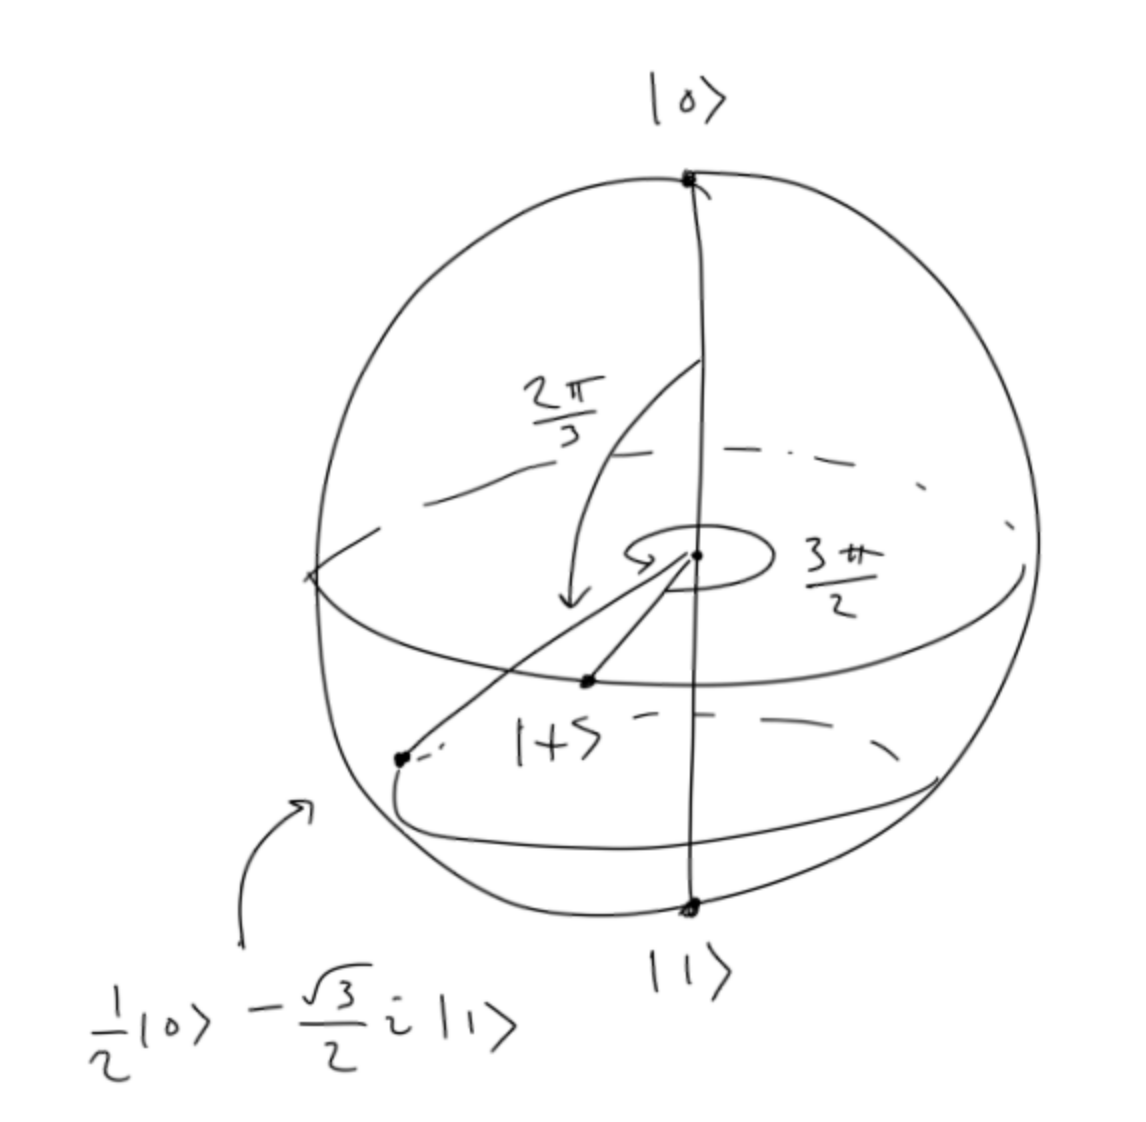
\includegraphics[width=2in]{review8blochsphere.png}
\end{center}
\end{solution}

\item Determine the expression for $| i \rangle$ in terms of the basis $\zeroket$, $\oneket$.  To do this, use the Bloch sphere (find $|i \rangle$ on the picture of the sphere and figure out the angles needed).
\item Determine the expression for $| i \rangle$ in terms of the basis $\plusket$, $\minusket$.  To do this, use linear algebra, knowing already how to write $i\rangle$, $\plusket$ and $\minusket$ in terms of $\zeroket$ and $\oneket$.
\item If $| i \rangle$ is measured in the basis $\plusket$, $\minusket$, what the probabilities and outcomes?  (use the last problem)
\item Consider the following state:
\[
|\psi \rangle =
\frac{ e^{i \pi/6}  }{\sqrt{3}} |0 \rangle +
\frac{ \sqrt{2} e^{-i \pi/4} }{\sqrt{3}} |1 \rangle
\]
\begin{enumerate}
    \item Check that it is normalized.
    \item Determine the probabilities and outcomes for measuring this state.
\end{enumerate}

\begin{solution}
To check that it is normalized, we compute
\[
|a|^2 + |b|^2 =
\left| \frac{ e^{i \pi/6}  }{\sqrt{3}}  \right|^2 + 
\left| \frac{ \sqrt{2} e^{-i \pi/4} }{\sqrt{3}} \right|^2
=
\left| e^{i \pi/6} \right|^2
\left| \frac{  1 }{\sqrt{3}}  \right|^2 + 
\left|e^{-i \pi/4} \right|^2
\left| \frac{ \sqrt{2}  }{\sqrt{3}} \right|^2
=
\left| \frac{  1 }{\sqrt{3}}  \right|^2 + 
\left| \frac{ \sqrt{2}  }{\sqrt{3}} \right|^2
= 
\frac{1}{3} + \frac{2}{3} = 1.
\]
So yes, it is normalized.

Probabilities:  If we measure this state in the $\zeroket$, $\oneket$ basis, we obtain $\zeroket$ with probability $1/3$ and $\oneket$ with probability $2/3$ (I'm reading this off from the computation we just did).

Outcomes:  If we measure $\zeroket$, then the state collapses to $\zeroket$.  If we measure $\oneket$, then the state collapses to $\oneket$.
\end{solution}

\item Here's a 3-qubit state:
\[
|\psi \rangle =
\frac{\sqrt{3}}{4} |000\rangle +
\frac{1}{4} |001\rangle +
\frac{1}{2\sqrt{2}} |010\rangle +
\frac{1}{2\sqrt{2}}  |011\rangle +
\frac{1}{2\sqrt{2}}  |100\rangle +
\frac{1}{2\sqrt{2}}  |101\rangle +
\frac{1}{2\sqrt{2}}  |110\rangle +
\frac{1}{2\sqrt{2}}  |111\rangle.
\]
\begin{enumerate}
    \item Measure all three qubits.  What is the probability of obtaining $001$?
    \item If you do indeed obtain $001$, what is the resulting collapsed state after measurement?
    \item Now reset your state afresh.  Now measure only the last qubit.  What is the probability of obtaining $1$?
    \item Assuming you do get $1$, what is the state after that measurement?
\end{enumerate}
\item Is each of the following states entangled?  If so, explain why.  If not, find the two independent single-qubit states:
\begin{enumerate}
    \item $\frac{1}{2}\left( 
    | 00 \rangle +
    i| 01 \rangle +
    i| 10 \rangle 
    -| 11 \rangle
    \right)$
    \item $\frac{1}{5}\left( 
      3| 01 \rangle 
    -4| 10 \rangle
    \right)$
    \item $\frac{1}{\sqrt{3}}\left( 
      | 00 \rangle 
      -| 01 \rangle 
    +| 11 \rangle
    \right)$    
\end{enumerate}
    \item Consider the matrix
    \[
    U = 
    \begin{pmatrix} 
    \frac{1}{\sqrt{2}} & \frac{i}{\sqrt{2}} \\
    \frac{i}{\sqrt{2}} & \frac{1}{\sqrt{2}} \\
    \end{pmatrix}
    \]
    Consider the state
    \[
    | \psi \rangle=
    \left( \frac{1}{2} + \frac{i}{2} \right) \zeroket
    +
    \left( \frac{1}{2} - \frac{i}{2} \right) \oneket
    \]
    \begin{enumerate}
    \item compute the probabilities and outcomes for a measurement of $|\psi\rangle$.
        \item compute the conjugate transpose $U^\dagger$ of $U$
        \item show $U$ is unitary
        \item apply $U$ to $| \psi \rangle$ and determine the outcome $U | \psi \rangle$.
        \item compute the probabilities and outcomes for a measurement of $U|\psi \rangle$.        %https://courses.cs.washington.edu/courses/csep590/05su/hw1sol.pdf
    \end{enumerate}

    \item You have a two-qubit system.  You first apply a Hadamard gate to the first qubit, then a Pauli Z gate to the second qubit (i.e., `phase flip' taking $\zeroket$ to $\zeroket$ but $\oneket$ to $-\oneket$).
    \begin{enumerate}
        \item Determine the $4 \times 4$ matrix that represents the resulting quantum circuit (i.e. the effect of doing both things in sequence as described above).
        \item Check that it is unitary.
    \end{enumerate}
    \item Write out the $4 \times 4$ QFT, and apply it to the Bell state.
    \item Explain the probability that any given bit is corrupted if Eve listens in on QKD.  What is the probability Eve measures the same bit as the bit sent?
    \item Be able to do QKD, e.g. play the role of Alice or Bob.
    \item Here is a quantum state in superposition.  What is the resulting state if I measure the second register?
    \[
    \frac{1}{\sqrt{m}} \sum_{i=0}^{m-1} |x\rangle |f(x) \rangle.
    \]
    \item Compute the continued fraction expansion of $171/1024$, and the good approximations.
    % [0, 1/5, 1/6, 85/509, 171/1024]
    \item Suppose you wish to factor $N=77$ with Shor's algorithm
    \begin{enumerate}
        \item How many qubits should you use according to the description of the algorithm?
        \item For the purposes of simulation, let's use $10$ qubits in the first register, and $6$ qubits in the second register.
        Let $\alpha = 3$.  Suppose you run the quantum part of the algorithm and you obtain a final measurement of $y=921$.  Complete the rest of the algorithm and discover a proper factor of $N$.
    \end{enumerate}

    \begin{solution}
    For part (a), we need to choose $m_0$ qubits so that $m = 2^{m_0} > N^2$.  Since $77^2 = 5929$, the next power of $2$ above that is $2^{13} = 8192$.  Hence we need $13$ qubits.
    \end{solution}

    \item Suppose you wish to factor $N=65$ using Shor's algorithm.  You use $10$ qubits in the first register and $6$ qubits in the second register.  You use $\alpha = 11$.  The final measurement on the quantum computer is $y=171$.  Complete Shor's algorithm to factor $N$.

    \begin{solution}
    Since we have $10$ qubits in the first register, $m = 2^{10} = 1024$.  We measure $y=171$, so we are searching for $r$ such that
    \[
        \frac{y}{m} \approx \frac{c}{r}.
    \]
    Thus we take the continued fraction expansion of $171/1024$.  This is
    \[
    0 + \frac{1}{
    5 + \frac{1}{
    1 + \frac{1}{
    84 + \frac{1}{
    2
    }
    }
    }
    }
    \]
    Therefore, the rational approximations are
    \[
    0 ,
    0 + \frac{1}{
    5 
    } = \frac{1}{5},
    0 + \frac{1}{
    5 + \frac{1}{
    1 
    }
    } = \frac{1}{6},
    0 + \frac{1}{
    5 + \frac{1}{
    1 + \frac{1}{
    84 
    }
    }
    }
     = \frac{85}{509},
    0 + \frac{1}{
    5 + \frac{1}{
    1 + \frac{1}{
    84 + \frac{1}{
    2
    }
    }
    }
    } = \frac{171}{1024}
    \]
    The denominators are
    \[
    5, 6, 509, 1024.
    \]
    We ignore the 1024, because that's just $m$.  We test the even ones to see if they work.  In this case, that is $r=6$.  Since we have $\alpha = 11$, we compute
    \[
    \gcd(\alpha^{r/2}-1,N)
    = \gcd(11^3-1, 65) = \gcd(1330,65) = 5.
    \]
    We have found a factor of 65, namely 5.
    \end{solution}
\end{enumerate}



\section{Lattice-based cryptography}

\subsection{Lattices and hard problems}

\subsection{Lattice reduction}

In two dimensions, a basis has two elements.  We play these two elements off of one another, trying to make them more perpendicular.

For this we will need to do some projecting of vectors.  Let us recall the definition.  The \emph{projection of $\mathbf{w}$ onto $\mathbf{v}$} is
\[
\operatorname{proj}_\mathbf{v}(\mathbf{w}) := \frac{ \mathbf{v} \cdot \mathbf{w} }{ \mathbf{v} \cdot \mathbf{v} } \mathbf{v}.
\]
That is, it is the component of $\mathbf{w}$ in the direction of $\mathbf{v}$.  Note that this is a scalar multiple of $\mathbf{v}$; the fraction out front is a scalar.

We will actually need to project more often on the orthogonal complement of $\mathbf{v}$.  We will denote this by $\operatorname{oproj}_\mathbf{v}(\mathbf{w})$; Wikipedia calls this the \emph{rejection}.  It is given by the formula:
\[
\operatorname{oproj}_\mathbf{v}(\mathbf{w}) := \mathbf{w} - \frac{ \mathbf{v} \cdot \mathbf{w} }{ \mathbf{v} \cdot \mathbf{v} } \mathbf{v}.
\]
Note here that the fraction of dot products is a scalar multiple, so we are taking an appropriate scaling of $\mathbf{v}$ from $\mathbf{w}$.  In particular, we are taking away the projection of $\mathbf{w}$ onto $\mathbf{v}$, leaving behind the component of $\mathbf{w}$ that is perpendicular to $\mathbf{v}$.

Let us now describe lattice reduction in two dimensions.  Suppose we begin with a basis $\mathbf{v}_1$, $\mathbf{v}_2$.
\begin{enumerate}
\item Reorder the basis if necessary so that $||\mathbf{v}_1|| \le ||\mathbf{v}_2||$.
\item We would like to replace $\mathbf{v}_2$ with $\mathbf{v}_2^*$ (to obtain a new basis $\mathbf{v}_1$, $\mathbf{v}_2^*$ which is `more perpendicular' to $\mathbf{v}_1$.  We might try $\mathbf{v}_2^* = \operatorname{oproj}_{\mathbf{v}_1}(\mathbf{v}_2)$, but the scalar multiple of $\mathbf{v}$ must be in the lattice, in order to obtain a new basis for the same lattice, and this is not guaranteed by the formula for projection.  Instead, we let
\[
\mathbf{v}_2^* := \mathbf{v}_2 - \left[ \frac{ \mathbf{v}_1 \cdot \mathbf{v}_2 }{ \mathbf{v}_1 \cdot \mathbf{v}_1 } \right] \mathbf{v}_1.
\]
Notice that this differs from $\operatorname{oproj}_{\mathbf{v}_1}(\mathbf{v}_2)$ only in the symbol $[]$ which indicates \emph{closest integer}.  In other words, we perform the orthogonal projection as usual, except we take the closest integer multiple of $\mathbf{v}_1$.
\item Return to step $1$, continuing this loop until
\[
\left[ \frac{ \mathbf{v}_1 \cdot \mathbf{v}_2 }{ \mathbf{v}_1 \cdot \mathbf{v}_1 } \right] = 0.
\]
(If this condition occurs, then $\mathbf{v}_2^* = \mathbf{v}_2$ and we would get stuck in an infinite loop.)
\end{enumerate}

Because the change of basis we have performed in step 2 is of the form
\[
\begin{pmatrix}
1 & \left[ \frac{ \mathbf{v}_1 \cdot \mathbf{v}_2 }{ \mathbf{v}_1 \cdot \mathbf{v}_1 } \right]  \\
0 & 1
\end{pmatrix},
\]
it has determinant $1$, and so $\mathbf{v}_1$, $\mathbf{v}_2^*$ is a basis of the same lattice.  The hope is that we have improved the orthogonality of our basis.  We repeat until we can no longer improve it.  To give some terminology to this condition (that the basis can no longer be improved), we say that $\mathbf{v}_1$, $\mathbf{v}_2$ is a \emph{reduced} basis whenever $||\mathbf{v}_1|| \le ||\mathbf{v}_2||$ and 
\[
\left[ \frac{ \mathbf{v}_1 \cdot \mathbf{v}_2 }{ \mathbf{v}_1 \cdot \mathbf{v}_1 } \right] = 0.
\]
Thus the algorithm produces a reduced basis.


Here is a worked example.

Let 
\[
\mathbf{v}_1 = \begin{pmatrix} 17 \\ 5 \end{pmatrix}, 
\mathbf{v}_2 = \begin{pmatrix} 19 \\ 10 \end{pmatrix}.
\]
Before we begin the example, let us compute the covolume, or determinant, of this lattice:
\[
\left| 
\begin{matrix}
17 & 19 \\
5 & 10
\end{matrix}
\right|
=
170 - 95 = 75.
\]
It will be useful to be able to double-check that this determinant is not changing, as a way to catch errors during the computation.

\textbf{Iteration 1}.  First we check the lengths of the vectors, so we can reorder if needed:
\[
|| \mathbf{v}_1 ||^2 = 17^2 + 5^2  = 289 + 25 = 314, \quad
|| \mathbf{v}_2 ||^2 = 19^2 + 10^2  = 361 + 100 = 461.
\]
Thus they are already ordered so that $\mathbf{v}_2$ is larger; we do not need to reorder them.  

Next, we compute $\mathbf{v}_2^*$ (notice that the length computations above are useful as we'll need one of them in the formula):
\[
\mathbf{v}_2^* := \mathbf{v}_2 - \left[ \frac{ \mathbf{v}_1 \cdot \mathbf{v}_2 }{ \mathbf{v}_1 \cdot \mathbf{v}_1 } \right] \mathbf{v}_1
= 
\begin{pmatrix} 19 \\ 10 \end{pmatrix}
-
\left[
\frac{
19 \cdot 17 + 10 \cdot 5
}{
314
}
\right]
\begin{pmatrix} 17 \\ 5 \end{pmatrix}
=
\begin{pmatrix} 19 \\ 10 \end{pmatrix}
-
\left[
\frac{
373
}{
314
}
\right]
\begin{pmatrix} 17 \\ 5 \end{pmatrix}
=
\begin{pmatrix} 19 \\ 10 \end{pmatrix}
-
1 \cdot
\begin{pmatrix} 17 \\ 5 \end{pmatrix}
=
\begin{pmatrix} 2 \\ 5 \end{pmatrix}.
\]
Thus our new basis is
\[
\mathbf{v}_1 = \begin{pmatrix} 17 \\ 5 \end{pmatrix}, 
\mathbf{v}_2^* = \begin{pmatrix} 2 \\ 5 \end{pmatrix}.
\]
We should double-check the determinant is still correct:
\[
17 \cdot 5 - 2 \cdot 5 = 85 - 10 = 75.
\]

\textbf{Iteration 2}.  The squared lengths of the two vectors are $314$ (from before) and $2^2 + 5^2 = 29$.  Clearly the second is the shorter, so we will reorder to write:
\[
\mathbf{v}_1 = \begin{pmatrix} 2 \\ 5 \end{pmatrix}, 
\mathbf{v}_2* = \begin{pmatrix} 17 \\ 5 \end{pmatrix}.
\]
Then, as before, we compute $\mathbf{v}_2^*$:
\[
\mathbf{v}_2^* := \mathbf{v}_2 - \left[ \frac{ \mathbf{v}_1 \cdot \mathbf{v}_2 }{ \mathbf{v}_1 \cdot \mathbf{v}_1 } \right] \mathbf{v}_1
= 
\begin{pmatrix} 17 \\ 5 \end{pmatrix}
-
\left[
\frac{
17 \cdot 2 + 5 \cdot 5
}{
29
}
\right]
\begin{pmatrix} 2 \\ 5 \end{pmatrix}
=
\begin{pmatrix} 17 \\ 5 \end{pmatrix}
-
\left[
\frac{
59
}{
29
}
\right]
\begin{pmatrix} 2 \\ 5 \end{pmatrix}
=
\begin{pmatrix} 17 \\ 5 \end{pmatrix}
-
2 \cdot
\begin{pmatrix} 2 \\ 5 \end{pmatrix}
=
\begin{pmatrix} 13 \\ -5 \end{pmatrix}.
\]
Thus our new basis is
\[
\mathbf{v}_1 = \begin{pmatrix} 2 \\ 5 \end{pmatrix}, 
\mathbf{v}_2^* = \begin{pmatrix} 13 \\ -5 \end{pmatrix}.
\]
We should double-check the determinant is still correct:
\[
2 \cdot (-5) - 13 \cdot 5 = -10 - 65 = -75.
\]
The sign difference is ok; this is still a basis (the sign will change when we reorder the vectors).

\textbf{Iteration 3}.  The squared lengths of the two vectors are $29$ (from before) and $13^2 + 5^2 = 194$.  No reordering is necessary, so we call them:
\[
\mathbf{v}_1 = \begin{pmatrix} 2 \\ 5 \end{pmatrix}, 
\mathbf{v}_2 = \begin{pmatrix} 13 \\ -5 \end{pmatrix}.
\]
Then, as before, we compute $\mathbf{v}_2^*$:
\[
\mathbf{v}_2^* := \mathbf{v}_2 - \left[ \frac{ \mathbf{v}_1 \cdot \mathbf{v}_2 }{ \mathbf{v}_1 \cdot \mathbf{v}_1 } \right] \mathbf{v}_1
= 
\begin{pmatrix} 13 \\ -5 \end{pmatrix}
-
\left[
\frac{
13 \cdot 2 + (-5) \cdot 5
}{
29
}
\right]
\begin{pmatrix} 2 \\ 5 \end{pmatrix}
=
\begin{pmatrix} 13 \\ -5 \end{pmatrix}
-
\left[
\frac{
1
}{
29
}
\right]
\begin{pmatrix} 2 \\ 5 \end{pmatrix}
=
\begin{pmatrix} 13 \\ -5 \end{pmatrix}
-
0 \cdot
\begin{pmatrix} 2 \\ 5 \end{pmatrix}
=
\begin{pmatrix} 13 \\ -5 \end{pmatrix}.
\]
Nothing has changed!  In fact, we got the scalar factor of $0$ which tells us that the basis is reduced.  (We might have twigged to this earlier because we found we didn't need to swap the vectors, so we are effectively trying to `orthogonalize' the second vector twice, which isn't going to improve matters.)

So we are done and our reduced basis is:
\[
\mathbf{v}_1 = \begin{pmatrix} 2 \\ 5 \end{pmatrix}, 
\mathbf{v}_2 = \begin{pmatrix} 13 \\ -5 \end{pmatrix}.
\]

\subsection{Regev Encryption}

\KS{in progress}

We've seen a few cryptosystems built on the general framework of El Gamal:  build a public/private key pair for two parties where
\begin{enumerate}
    \item Having the private info for one party and the public info for the other allows computation of a shared secret;
    \item The shared secret is used as a mask on a message.
\end{enumerate}

Regev encryption follows this model, and it uses linear algebra for the underlying `math world' to work in.

Let $p$ be a large prime, and $k > n$ two moderate integers.  We will work in two vector spaces over the finite field $\FF_p := \ZZ/p\ZZ$, namely $\FF_p^n$ and $\FF_p^k$.  The computations will all be linear algebra (matrix multiplication).

Bob's public/private key pair is the following:
\begin{enumerate}
    \item A secret vector $s \in \FF_p^n$ (used for decryption)
    \item A secret error $e \in \FF_p^k$ (which should have small entries, but won't be used later)
    \item A public $k \times n$ matrix with entries in $\FF_p$.
\end{enumerate}

The public key is $A, b:= As + e \in \FF_p^k$.

\KS{todo draw little diagrams like in notes}

\subsubsection{Regev Encryption Algorithm}

     {\bf Setup:}  $p$, $k > n$
     \vspace{1em}

     \begin{tabular}{ccc}
       Alice & & Bob \\
       \hline
       Message: $m \in \{0,1\}$ & &  Secret key: $s \in \FF_p^n$ \\
       & & Error: $e \in \FF_p^k$ small \\
       $(A,b)$ & $\longleftarrow$ & Public key: $(A, b = As+e)$ \\
       Ephemeral secret key: $r \in \FF_p^k$ small & &  \\
       Ephemeral public key: $d = r^T A \in \FF_p^n$ & &  \\
       Masked message: $c = r^T b + m(p-1)/2$ & &  \\
       Ciphertext: $(d,c)$ & $\longrightarrow$ & $(d,c)$ \\
					      & & Decryption: $c - ds \in \FF_p$ \\
                          & & if in $(-p/4,p/4)$, message = 0 \\
                          & & otherwise, message = 1
      \end{tabular}
      \vspace{3em}

      To verify that the algorithm is correct, observe:
      \[
      c - ds = m\left( \frac{p-1}{2} \right) + r^T(As+e) - r^TAs
      = m\left(\frac{p-1}{2}\right) + r^Te.
      \]
      This is not \emph{exactly} the message, but the number $r^Te$ should be fairly small compared to $p$, so that it should still decrypt (by rounding) to the correct bit.

\subsubsection{Simple example}

\begin{enumerate}
    \item Let's let $p=7$, $n=2$, $m=3$.  
    \item Suppose Alice wishes to send the message bit $1$.
    \item Bob chooses random private key $s = \begin{pmatrix}1\\4\end{pmatrix} \in \FF_7^2$.
    \item Bob chooses random \textbf{small} error vector $e = \begin{pmatrix} -1 \\ 0 \\ 1 \end{pmatrix} \in \FF_7^3$.
    \item Bob chooses random public matrix $A = \begin{pmatrix} 0 & 1 \\ 3 & 2 \\ 5 & 5 \end{pmatrix}$.
    \item Bob computes $b = As + e = \begin{pmatrix} 0 & 1 \\ 3 & 2 \\ 5 & 5 \end{pmatrix}\begin{pmatrix}1\\4\end{pmatrix} +\begin{pmatrix} -1 \\ 0 \\ 1 \end{pmatrix} = 
    \begin{pmatrix} 4 \\ 4 \\ 4 \end{pmatrix}+
    \begin{pmatrix} -1 \\ 0 \\ 1 \end{pmatrix}=
    \begin{pmatrix} 3 \\ 4 \\ 5 \end{pmatrix}$.
    \item This pair $(A,b)$ is sent to Alice.
    \item Alice chooses random \textbf{small} ephemeral private $r = \begin{pmatrix} 1 \\ 0 \\ 1 \end{pmatrix} \in \FF_7^3$.
    \item Alice computes public $d = r^TA = 
    \begin{pmatrix} 1 & 0 & 1 \end{pmatrix}\begin{pmatrix} 0 & 1 \\ 3 & 2 \\ 5 & 5 \end{pmatrix}$.  (The exponent $T$ is transpose.)
    \item Alice computes the mask $r^T b =  \begin{pmatrix} 1 & 0 & 1 \end{pmatrix} \begin{pmatrix} 3 \\ 4 \\ 5 \end{pmatrix} =  1$.
    \item Alice adds the mask to the message to obtain ciphertext: $c = r^Tb + m(p-1)/2 = 1 + 3 = 4 \in \FF_7$.
    \item Alice sends $(d,c)$ to Bob.
    \item Bob computes his version of the mask $ds = \begin{pmatrix} 5 & 6 \end{pmatrix} \begin{pmatrix} 1 \\ 4 \end{pmatrix} = 1$.
    \item Bob subtracts the mask from the ciphertext: $c-ds = 4 - 1 = 3$.
    \item Bob find that this is closer to $(p-1)/2$ than to $0$ on the mod $7$ ``cycle" so he rounds this to recover the message bit, i.e. $1$.
\end{enumerate}





\subsection{Learning with Errors}

Learning with Errors is not directly based on the Short Vector Problem or the Closest Vector Problem, although the problem is closely related to those.

Like other cryptosystems we have seen, to work in a finite system, we work modulo $p$ for some large $p$.  In our case, this means we are doing linear algebra over the field $\mathbb{F}_p$.

The fundamental hard problem is based on a linear system with `errors' posed in high dimension, and is called the \emph{Learning with Errors} problem.  It concerns an equation of the following form:
\[
A \mathbf{s} = \mathbf{b} + \mathbf{e}.
\]
In this system, $A$ is a $k \times n$ matrix, $k > n$, $\mathbf{s}$ is a vector of length $n$, and $\mathbf{b}, \mathbf{e}$ are vectors of length $k$.  Additionally, $\mathbf{e}$ has small entries.  The matrix $A$ and vector $\mathbf{b}$ are known; the secret is $\mathbf{s}$.  The `error' $\mathbf{e}$ is also unknown.  The hard problem is to find $\mathbf{s}$. \KS{draw this diagram style showing dimensions}

Some observations on this problem:
\begin{enumerate}
    \item If there were no error $\mathbf{e}$, Gaussian elimination would solve this.
    \item Consider Figure \KS{make fig}; if we take any $n$ of the $k$ rows of $A$, we form a smaller linear system $A' \mathbf{s} = \mathbf{b}' + \mathbf{e}'$.  This implies that $\mathbf{s}$ is in the image of $A'^{-1}(R)$ where $R$ is a small region surrounding $\mathbf{b}'$ formed of all possible vectors $\mathbf{b}' + \mathbf{e}'$, where $\mathbf{e}'$ has small entries.
    \item In high dimensions, the volume of this small region is exponentially large.
\end{enumerate}

\textbf{The Search Learning-with-Errors Problem}.  Suppose we are given a $k \times n$ matrix $A$ with entries in $\FF_p$, such that $k > n$, and a vector $\mathbf{b} \in \FF_p^k$, such that $A \mathbf{s} = \mathbf{b} + \mathbf{e}$ for some $\mathbf{s} \in \FF_p^n$ and $\mathbf{e} \in \FF_p^n$ with small entries.  Find $\mathbf{s}$.

There is also a decisional variant.

\textbf{The Decision Learning-with-Errors Problem}.  Suppose we are (repeatedly) given a $k \times n$ matrix $A$ with entries in $\FF_p$, such that $k > n$, and a vector $\mathbf{b} \in \FF_p^k$, such that either (a) $A \mathbf{s} = \mathbf{b} + \mathbf{e}$ for some $\mathbf{s} \in \FF_p^n$ and $\mathbf{e} \in \FF_p^n$ with small entries, or (b) $A$ and $\mathbf{b}$ are unrelated and uniformly random.   Be able to determine, under repeated trials, with probability significantly greater than $1/2$, which of these is the case (i.e. whether $\mathbf{s}$ exists for each pair $(A, \mathbf{b})$).

In fact, there are reductions both direction between certain precise versions of Learning with Errors and the standard lattice problems like SVP.


Some ways we might na\"ively attack this problem:
\begin{enumerate}
\item Search for $\mathbf{s}$ exhaustively.  The secret $\mathbf{s}$ could be any vector in $\FF_p^n$, i.e. there are $p^n$ possibilities.
\item Search for $\mathbf{e}$ exhaustively; for each possibility for $\mathbf{e}$, check if the system is consistent (i.e. there exists a solution $\mathbf{s}$).  Since $k > n$, for most choices of $\mathbf{e}$, there is likely no solution to this overdetermined system.  There are $k^n$ possibilities for $\mathbf{e}$, where $k$ is the number of possibilities for each entry.  For example, if `small' means entries from $\{ -1, 0, 1 \}$, then we will have $3^n$ possibilities.  This is still exponential in the dimension.
\end{enumerate}

There are other attacks on this problem, including reductions to the more standard lattice problems.  For example, if we consider the lattice
\[
\Lambda = \{ 
\mathbf{y} \in \ZZ^k : \mathbf{y}^t A \equiv \mathbf{0} \pmod p \},
\]
and we find a short vector in this lattice, say $\mathbf{y}$, then
\[
\mathbf{y}^t \mathbf{b}
= 
\mathbf{y}^t (A\mathbf{s}  + \mathbf{e})
= 
\mathbf{y}^t A\mathbf{s} + 
\mathbf{y}^t \mathbf{e}
=
0
+ \mathbf{y}^t \mathbf{e} \pmod{p}.
\]
If $\mathbf{e}$ is small, then this is a small number modulo $p$.  Otherwise, we expect it to be uniformly distributed modulo $p$.  This allows us to solve the \emph{Decision Learning with Errors} problem.

\subsection{Ring-LWE}

Define $R_p$ etc.

\subsection{Ring-LWE Public Key Cryptosystem}

This system is modelled after El Gamal, but using public private key pairs of the form:

Private key:  $b \in R_p$

Public key: $(g, B = gb + e)$

This is in analogy to the private public key pair $b$ and $g^b$ in Diffie-Hellman.  One difference here is that we use a new $g$ each time, instead of setting one for all time as a public parameter of the system, so $g$ is included in the public key.  Another difference is that to protect the secret $b$, we need to add an error $e$, whose large space of possibilities is what makes the problem of recovering $b$ hard.

Therefore, the following are the public parameters:
\begin{enumerate}
\item $p$ a moderately large prime
\item $n$ a moderately large integer
\item $R_p = \FF_p[x]/(x^n+1)$, the ring
\item a notion of `small', e.g. $\{-1,0,1\}$ for error coefficients
\item an integer $\ell < p$ which is moderately large.
\end{enumerate}

With this set up, a message $m \in R_p$ is chosen so its coefficients are in the range
\[
0 < m < p/\ell.
\]

Key exchange proceeds as follows:
\begin{enumerate}
\item Bob creates and shares a public key:
\begin{enumerate}
\item Bob creates a private key $b \in R_p$ which is small and random.
\item Bob creates a public key $(g, B = gb + e)$ where $g \in R_p$ is random and $e_1$ is an error (small and random).
\end{enumerate}
\item Alice encrypts using Bob's public key:
\begin{enumerate}
\item Alice creates an ephemeral private key $k \in R_p$ which is small and random.
\item Alice creates an ephemeral public key $K = gk + e_2$ where $e_2$ is an error and $g$ is taken from Bob's public key.
\item Alice creates a ciphertext
\[
C = Bk + e_3 + m\ell
\]
where $Bk+e_3$ plays the role of a shared Diffie-Hellman-like key which masks the message $m\ell$ (we'll see in a moment why $m$ is stored as a multiple of $\ell$).
\item Alice sends $(K,c)$ as the encrypted message.
\end{enumerate}
\item Bob decrypts Alice's message using his private key:
\begin{enumerate}
\item Bob computes
\[
C - Kb;
\]
this is like computing his version of the shared Diffie-Hellman-like key as $Kb$ and subtracting off the mask.
\item Then rounds the result to the nearest multiple of $\ell$
\item Then divides off the factor of $\ell$.
\end{enumerate}
\end{enumerate}

To see that Bob's decryption recovers the message, we compute:
\[
C - Kb = m\ell + (g b + e_1) k + e_3 - (gk + e_2) b
= m \ell + (ke_1 + e_3 - be_2).
\]
The bracketed quantity at right is small, as it is a combination of small things.  Therefore when rounding, we will obtain $m\ell$, so that dividing by $\ell$, we obtain $m$.

We might wonder about a key difference from the El Gamal system:  why Bob has to generate $g$ as part of his public key.  The answer is that if we re-use $g$ for lots of private/public key pairs, there are some attacks that can exploit this.  It's more protective to keep $g$ changing. \KS{maybe expand here}

\subsection{Ring-LWE Example}

Parameters:
\begin{align*}
	n &= 4 \\
	p &= 101 \\
	\ell &= 20 
\end{align*}
In particular,
\[
R_p = \FF_p[x]/(x^4+1),
\]
whose elements looks like polynomials in $x$ with degree at most $3$ and coefficients modulo $p$.

For this example, the meaning of small will be coefficients from $\{1,0,-1\}$.  Therefore, the small elements of $R_p$ are
\[
\{ a x^3 + b x^2 + cx + d : a,b,c,d \in \{100,0,1\} \}.
\]
(Notice that $100 \equiv -1 \pmod p$.)

Let's send a message; let's say $m = 3$.

\begin{enumerate}
\item Bob's Key Generation:
\begin{enumerate}
\item Bob's private key:
\[
	b = x^3 + 100
\]
\item Create an error for use in public key:
\[
	e_1 = x^3 + x^2 + 100x
\]
The Public key is
\begin{align*}
	g &= 83x^3 + 23x^2 + 51x + 77 \\
	B &= gb + e_1 = 96x^3 + 97x^2 + 26x + 74 \\
\end{align*}
\end{enumerate}
\item Alice's Encryption 
\begin{enumerate}
\item Ephemeral private key:
\[
	k = 100x^2 + 100x
\]
\item Create error for use in ephemeral public key:
\[
e_2 = x^2
\]
Ephemeral public key:
\begin{align*}
	K &= gk + e_2 = 27x^3 + 75x^2 + 6x + 5 % AI-FIXED: was gk + e_1
\end{align*}
\KS{Fixed by AI: the ephemeral public key is $K=gk+e_2$ (per the scheme definition), not $gk+e_1$. Verified: $gk+e_2=27x^3+75x^2+6x+5$ over $\FF_{101}[x]/(x^4+1)$, matching the stated value.}
\item Create error for us in ciphertext:
\[
e_3 = 100x^2 + x
\]
Ciphertext:
\begin{align*}
	  C &= Bk + e_3 + \ell m = 79x^3 + 23x + 51 % AI-FIXED: was Bk + e_2
\end{align*}
\KS{Fixed by AI: the ciphertext uses the error $e_3$ (per the scheme, $C=Bk+e_3+\ell m$), not $e_2$. Verified: $Bk+e_3+\ell m=79x^3+23x+51$ over $\FF_{101}[x]/(x^4+1)$, matching the stated value.}
\end{enumerate}
\item {Bob's Decryption}
\begin{enumerate}
\item Decryption formula:
\[
	C - Kb = x^2 + 3x + 62
\]
\item Rounding to the nearest $\ell=20$, we get
\[
	60 = 3 \ell
\]
\item Therefore the message is $3$.
\end{enumerate}
\end{enumerate}


\section{Coding Theory}

\subsection{Principles and terminology}

\KS{terminology \& basic ideas like code, codeword, length, error correction, etc.}

\subsection{Hamming distance}

Think of errors as gradually modifying a binary string, one bit at a time.  Remember these fun word ladder games you played as a kid?
\begin{align*}
&TEXT \\
&TEST \\
&LEST \\
&LOST \\
&LOSE \\
&NOSE \\
&NODE \\
&CODE
\end{align*}

In a language of all binary strings, there's no restriction that any step be a word, so we define the \textbf{Hamming distance} $d(u,v)$ to be the number of positions at which two strings $u$ and $v$ differ.  For example
\[
d(000111,001011) = 2
\]
because they differ at two positions (in the middle).  The use of the word `distance' is meant to invoke this idea of how many `steps' it takes to travel from one string to the other via letter changes.  One such path is:
\[
000111 \rightarrow 001111 \rightarrow 001011.
\]
It's the `distance' in the sense of being the \emph{shortest} path.  It also has a number of properties that align with our intuitive notion of `distance', namely:
\begin{enumerate}
    \item Distances cannot be negative: $d(u,v) \ge 0$.
    \item Distance is zero if and only if the two strings are equal: $d(u,v) = 0 \Leftrightarrow u=v$.
    \item The distance is symmetric:  $d(u,v) = d(v,u)$.
    \item The distance cannot get shorter by adding a waypoint: $d(u,v) \le d(u,w) + d(w,v)$ (triangle inequality).
\end{enumerate}
These properties mean that, mathematically speaking, the Hamming distance is a metric.

\begin{quiz}
    Prove these properties.
\end{quiz}
\begin{aisolution}
Write $d(u,v)$ for the number of positions $i$ at which $u_i \neq v_i$.
\begin{enumerate}
\item $d(u,v) \geq 0$ because it is a count of positions, which cannot be negative.
\item $d(u,v) = 0$ means there are \emph{no} positions where $u$ and $v$ differ, which is exactly the statement that $u = v$ (and conversely, equal strings differ nowhere).
\item Symmetry: the position $i$ satisfies $u_i \neq v_i$ if and only if $v_i \neq u_i$, so the two counts $d(u,v)$ and $d(v,u)$ are equal.
\item Triangle inequality: consider any position $i$ counted by $d(u,v)$, i.e. $u_i \neq v_i$.  Then we cannot have both $u_i = w_i$ and $w_i = v_i$ (that would force $u_i = v_i$).  Hence $i$ is counted by $d(u,w)$ or by $d(w,v)$ (or both).  Summing over all such positions, $d(u,v) \leq d(u,w) + d(w,v)$.
\end{enumerate}
\end{aisolution}

Wikipedia has a cool Hamming distance visualization!

\url{https://en.wikipedia.org/wiki/Coding_theory}

The \textbf{distance} of a code is the minimum distance between its codewords.

If two binary codewords lie at distance $d$ from one another, then it takes at least $d$ bit flips, or errors, to change one into the other.  Thus, for a code of distance $d$, any number of errors strictly less than $d$ can be detected.

As for codeword correction, I'm reminded of an old joke:  ``I was swimming across the 10 mile wide lake, but I got tired at 9 miles and turned around."  To correct errors via nearest neighbour decoding, we cannot tolerate `walking' half or more of the distance to the nearest codeword.  If we have gone at least halfway, a different codeword may now be our nearest neighbour -- we could correct to an incorrect codeword!  So we can correct at most $(d-1)/2$ errors.  We have proven the following.

\begin{proposition}
    If a code $\mathscr{C}$ has distance $d$, then it can detect $d-1$ errors, and correct $\lfloor \frac{d-1}{2} \rfloor$ errors.
\end{proposition}

\subsection{Some Example Codes}

\KS{The code $\{000,111\}$, the checksum code, and the Hamming codes we covered in class.}


\subsection{Vector spaces and cosets over finite fields}

Recall that when $p$ is prime, $\ZZ/p\ZZ$ is called a \textbf{finite field} (there are other finite fields too, but we'll stick to these).  To be a field means, in particular, that all non-zero elements are invertible.  This makes life particularly easy in a variety of ways, and it makes linear algebra work well (the most notable feature is that we can invert any matrix with non-zero determinant).  So we can consider a \textbf{vector space over a finite field}, $\FF_p^k$, which is a set of \textbf{vectors} having $k$ entries, each of which is taken modulo $p$.  For example,
\[
\FF_2^2 = \{ (0,0), (0,1), (1,0), (1,1) \}.
\]
\textbf{Cardinality of a vector space:}  Since there are $k$ entries, each of which can take one of $p$ values, the vector space $\FF_p^k$ has $p^k$ elements.

One particularly useful idea in this context is the notion of a \textbf{subspace}, which is a vector space inside a vector space:  the definition of a subspace of $\FF_p^k$ is a non-empty subset that is closed under addition and scalar multiplication.  That means, if we take elements in the subspace and add or scale them, the results are also in the subspace.

\begin{quiz}
    Explain why the zero vector must be in any subspace.\footnote{Because scaling by zero results in the zero vector, and the definition of subspace says all scalings are also in the subspace.}
\end{quiz}
\begin{aisolution}
A subspace is nonempty, so it contains some vector $v$.  A subspace is closed under scalar multiplication, so it must also contain $0\cdot v = \mathbf{0}$, the zero vector.  Hence every subspace contains $\mathbf{0}$.
\end{aisolution}

A subspace is itself a vector space \KS{does this need more explanation?  it isn't a standard form vector space, i.e. standard basis vectors}, so it has a \textbf{dimension}.  So the possible sizes of subspaces of $\FF_p^k$ are $1$ (the set of just the zero vector by itself), $p$ (lines), $p^2$ (planes), $p^3$, etc., up to $p^{k-1}$ and $p^k$ (the full space).

It helps to do a few examples of subspaces, which is where 3d Tic-Tac-Toe comes in.  \KS{insert pics from the course notes or a photo of the 3d tic tac toe or something!}

For example, here are all the lines through the origin in $\FF_3^2$: \KS{look at class notes}; these are all the subspaces of dimension $1$.

Notice (from above) that subspaces include the origin -- the zero vector.  So the lines that don't pass through the origin are not subspaces.  But they are still very `linear', so we will find them useful subsets to consider also.  These are examples of cosets.  A \textbf{coset} is a translation of a subspace.  Symbolically, if $V$ is a subspace, then $u + V$ is a coset for each possible vector $u$.

Again, an example helps.  Here are all the lines in $\FF_3^2$:

\KS{include a drawing}

A particularly nice property of cosets is that the full vector space can be broken up into disjoint cosets, once we've chosen a subspace.  Here's an example:

\KS{again there are pics in the course notes}

\begin{example}
\begin{enumerate}
    \item Consider the set $\{ 000, 010, 001, 100 \}$ as a subset of $\FF_2^3$.  Is this a subspace?  The answer is no.
        If it were a subspace, then any linear combination of the elements would have to be contained in the subspace also.  But $010 + 001 = 011$ which is not in the subspace.
        \item Consider the set $\{ 01, 10 \}$ as a subset of $\FF_2^2$.  Is this a subspace?  The answer is no.  If it were a subspace, it would include the zero vector.  \item Consider the set $\{ 00, 01, 10 \}$ as a subset of $\FF_2^2$.  Is this a subspace?  The answer is no.  If it were a subspace, it would have a power of two cardinality.
        \item Consider the set $\{ 000, 010, 001, 011 \}$ as a subset of $\FF_2^3$.  Is this a subspace?  The answer is yes.  To see this, you could check that all linear combinations stay inside the space.  Or you could give linear equations that describe the space, e.g., the set consists of all vectors $(x,y,z)$ such that $x=0$.
\end{enumerate}
\end{example}

\subsection{Linear Codes}

It can be helpful to give extra structure to codes.  Linear codes are codes that are also subspaces.  This means that when we add two codewords, the result is again a codeword.  This extra structure can make it easier to handle the codes:  compute the minimum distance, say, or encode and decode efficiently.

For example, the next proposition states that a linear code's minimum distance can be computed as the smallest Hamming weight of its non-zero elements.

\begin{proposition}
    The minimum distance of a linear code $\mathcal{C}$ is given by
    \[
    d(\mathcal{C}) = \{ wt(u) : u \in \mathcal{C}, u \neq 0\}.
    \]
\end{proposition}

This means that instead of comparing all possible pairs of codewords to find the minimum distance, we need only look at the individual codewords themselves.

\begin{example}
Consider this code in the vector space $\FF_2^4$:
\[
\mathbf{C} = \{ 0000, 1011, 0110, 1101 \}
\]
We will adopt the convention of writing vectors as strings (without the parentheses and commas) to save space.

This is a linear code.  This can be checked adding the vectors in all possible pairs to check they remain in the code\footnote{Another way to see this is to observe that $\mathbf{C}$ is exactly all the strings satisfying the linear conditions $v_1 = v_4$, $v_2+v_3+v_4 = 0$.}.
\end{example}

\subsubsection{Cosets}

A \textbf{coset} is a translation of a subspace.  That is, if you take $\mathbf{u}$ in the vector space, then the set
\[
\mathbf{u} + \mathbf{C} = \{ \mathbf{u} + \mathbf{x} : \mathbf{x} \in \mathbf{C} \}
\]
is called a coset.

For the code $\mathbf{C}$ in the example above, some cosets are:
\begin{align*}
     \mathbf{C} &= \{ 0000, 1011, 0110, 1101 \} \\
     1000+\mathbf{C} &= \{ 1000, 0011, 1110, 0101 \} \\
     0100+\mathbf{C} &= \{ 0100, 1111, 0010, 1001 \} \\
     0001+\mathbf{C} &= \{ 0001, 1010, 0111, 1100 \} 
\end{align*}

\begin{quiz}
    Check that
\[
0010+\mathbf{C} = 0100+\mathbf{C}.
\]
\end{quiz}
\begin{aisolution}
Computing the coset directly, $0010 + \mathbf{C} = \{0010,\,1001,\,0100,\,1111\}$, which is the same set of four strings as $0100 + \mathbf{C} = \{0100,\,1111,\,0010,\,1001\}$.  More cleanly: $0010 = 0100 + 0110$ and $0110 \in \mathbf{C}$, so $0010 \in 0100 + \mathbf{C}$; since two cosets that share an element are equal, $0010 + \mathbf{C} = 0100 + \mathbf{C}$.
\end{aisolution}

Cosets have some very nice properties.

\begin{proposition}
    Two cosets are either equal or disjoint.
\end{proposition}

\begin{proof}
    Suppose that $\mathbf{u} \in \mathbf{v} + \mathbf{C}$.  Then $\mathbf{u} = \mathbf{v} + \mathbf{c}$ for some codeword $\mathbf{c} \in \mathbf{C}$.  So we have
    \[
    \mathbf{u} + \mathbf{C} = 
    \mathbf{v} + \mathbf{c} + \mathbf{C} = \mathbf{v} + \mathbf{C}.
    \]
    Notice that we are using the fact that the code, translated by a codeword, returns the code.  This is from the definition of a subspace\footnote{There's a detail here!  Being a subspace means that adding a codeword to anything in $\mathbf{C}$ will give another element of $\mathbf{C}$.  This tells us $\mathbf{c} + \mathbf{C} \subseteq \mathbf{C}$.  This isn't quite enough.  But adding a vector to all elements of a set is an \emph{invertible} procedure, so we actually get a bijection between $\mathbf{c}+\mathbf{C}$ and $\mathbf{C}$, so they are equal.}.
    So we have shown that if two cosets intersect, then they are equal.
\end{proof}




\subsection{Cyclic Codes}

\subsection{McEliece Cryptosystem}


     {\bf Setup:}  $p$ prime, $k$ and $n$ dimensions
     \vspace{1em}

     \begin{tabular}{ccc}
       Alice & & Bob \\
       \hline
       Message: $m \in \FF_p^k$ & &  Secret key: $G$ a $k \times n$ matrix over $\FF_p$ \\
       & & $S$ a $k \times k$ invertible matrix over $\FF_p$ \\
       & & $P$ a $n \times n$ permutation matrix over $\FF_p$ \\
       $G_1$ & $\longleftarrow$ & Public key: $G_1 = SGP$ a $k \times n$ matrix over $\FF_p$ \\
       Ephemeral error: $e \in \FF_p^k$ \\
       having correctable Hamming weight & &  \\
       Ciphertext: $y = xG_1 + e$ & $\longrightarrow$ & $y$ \\
					      & & Decryption: \\
                          && $y_1 = yP^{-1} \in \FF_p^k$ \\
                          & & $= (xG_1+e)P^{-1}$ \\
                          & & $= xSG+e'$ \\
                          & & Decode $y$ to get $x_1 = xSG$ \\
                          & & Compute $x = x_0 S^{-1}$ 
      \end{tabular}
      \vspace{3em}

\subsection{Review Problems for Codes}

\begin{enumerate}
\item What is the Hamming weight of the binary vector $001110$?
\item In $\FF_3^3$, which of the following subsets are subspaces?  Why or why not?  For the ones which are, give examples of cosets.
\begin{enumerate}
    \item $\{000,111,222\}$
    \item $\{000\}$
    \item $\{010,002,001\}$
    \item $\{000,010,020,001\}$
\end{enumerate}
\item Create a binary code of length 4 with 5 codewords.  Can you create an example with large minimum distance?  Experiment and compare with your friends for largest minimum distance.  What is the code rate of your code?
\item Here's a nice linear binary code:
\[
G=
\begin{pmatrix}
    0 & 0 & 0 & 0 & 1 & 1 & 1 & 1 \\
    0 & 0 & 1 & 1 & 0 & 0 & 1 & 1 \\
    0 & 1 & 0 & 1 & 0 & 1 & 0 & 1 \\
\end{pmatrix}
\]
Work out:
\begin{enumerate}
    \item length
    \item dimension
    \item number of codewords
        \item minimum distance (remember this is a linear code, so there's an easier way to approach this)
            \item how many errors it can correct
    \item how many errors it can detect
        \item information rate
    \item put it in systematic form (you can reorder the columns) before doing the rest of this problem
    \item parity check matrix
    \item give an example of encoding, error and syndrome decoding (within the error correction range)
\end{enumerate}
    \item Hamming example.
    \begin{enumerate}
        \item Write out the [15,11]-Hamming code generating matrix and its parity check matrix in a systematic form.  
        \item Choose a codeword, and make an error in one position.  
        \item Then use the parity check matrix to find the syndrome.  
        \item Verify that syndrome decoding would recover the original codeword.
        \item Now make an error in two positions.  What does decoding produce?
        \item What is the minimum distance of a Hamming code (this is just fact check)?
    \end{enumerate}
    \item Write out the generating matrix for the single-checksum-bit checksum code example we did in class.  Explain why this is a linear code.
    \item %(from Trappe-Washington)
    Create a cyclic binary code with length $4$ using generating polynomial $g(X) = X^2+1$.  Check if the following polynomials are codewords or not:  $1+X+X^3$, $1+X+X^2+X^3$, $X^2+X^3$.
    \item Show that $\{ 000, 110, 011, 101 \}$ is a cyclic code by finding $n$ and $p$ and the polynomial $g(x)$.  Find the generating and parity check matrices.  How many errors can this code detect and how many can it correct?
\end{enumerate}


\section{Things to incorporate into updates}

\begin{enumerate}
    \item Boldyreva's Blind Signature
    \item BSM - Basic Safety Message (automated cards); Vehicle to Vehicle -- for signatures
    \item Falcon signature is fairly simple
    \item PS3 hack on the nonce
    \item NIST's new guidance to deprecate
    \item more emphasis on signatures (data integrity) used everywhere
\end{enumerate}

\end{document}

